%% Package and Class "uiucthesis2014" for use with LaTeX2e.
\documentclass[edeposit,fullpage]{uiucthesis2018}


\usepackage[acronym,toc]{glossaries}
\newacronym[longplural={metric tons of heavy metal}]{MTHM}{MTHM}{metric ton of heavy metal}
\newacronym{ABM}{ABM}{agent-based modeling}
\newacronym{ACDIS}{ACDIS}{Program in Arms Control \& Domestic and International Security}
\newacronym{AFCI}{AFCI}{Advanced Fuel Cycle Initiative}
\newacronym{AHTR}{AHTR}{Advanced High Temperature Reactor}
\newacronym{ANDRA}{ANDRA}{Agence Nationale pour la gestion des D\'echets RAdioactifs, the French National Agency for Radioactive Waste Management}
\newacronym{ANL}{ANL}{Argonne National Laboratory}
\newacronym{ARDP}{ARDP}{Advanced Reactors Demonstration Program}
\newacronym{API}{API}{application programming interface}
\newacronym{ARCH}{ARCH}{autoregressive conditional heteroskedastic}
\newacronym{ARE}{ARE}{Aircraft Reactor Experiment}
\newacronym{ARFC}{ARFC}{Advanced Reactors and Fuel Cycles}
\newacronym{ARMA}{ARMA}{autoregressive moving average}
\newacronym{ASME}{ASME}{American Society of Mechanical Engineers}
\newacronym{ATWS}{ATWS}{Anticipated Transient Without Scram}
\newacronym{BDBE}{BDBE}{Beyond Design Basis Event}
\newacronym{BIDS}{BIDS}{Berkeley Institute for Data Science}
\newacronym{BOL}{BOL}{Beginning-of-Life}
\newacronym{BSD}{BSD}{Berkeley Software Distribution}
\newacronym{BWR}{BWR}{Boiling Water Reactor}
\newacronym{CAFCA}{CAFCA}{ Code for Advanced Fuel Cycles Assessment }
\newacronym{CASL}{CASL}{Consortium for Advanced Simulation of Light Water Reactors}
\newacronym{CDTN}{CDTN}{Centro de Desenvolvimento da Tecnologia Nuclear}
\newacronym{CEA}{CEA}{Commissariat \`a l'\'Energie Atomique et aux \'Energies Alternatives}
\newacronym{CF}{CF}{capacity factor}
\newacronym{CI}{CI}{continuous integration}
\newacronym{CNEC}{CNEC}{Consortium for Nonproliferation Enabling Capabilities}
\newacronym{CNEN}{CNEN}{Comiss\~{a}o Nacional de Energia Nuclear}
\newacronym{CNERG}{CNERG}{Computational Nuclear Engineering Research Group}
\newacronym{COSI}{COSI}{Commelini-Sicard}
\newacronym{COTS}{COTS}{commercial, off-the-shelf}
\newacronym{CSNF}{CSNF}{commercial spent nuclear fuel}
\newacronym{CTAH}{CTAHs}{Coiled Tube Air Heaters}
\newacronym{CUBIT}{CUBIT}{CUBIT Geometry and Mesh Generation Toolkit}
\newacronym{CURIE}{CURIE}{Centralized Used Fuel Resource for Information Exchange}
\newacronym{DAG}{DAG}{directed acyclic graph}
\newacronym{DANESS}{DANESS}{Dynamic Analysis of Nuclear Energy System Strategies}
\newacronym{DBE}{DBE}{Design Basis Event}
\newacronym{DESAE}{DESAE}{Dynamic Analysis of Nuclear Energy Systems Strategies}
\newacronym{DHS}{DHS}{Department of Homeland Security}
\newacronym{DOE}{DOE}{Department of Energy}
\newacronym{DOE-NE}{DOE-NE}{U.S. Department of Energy, Office of Nuclear Energy}
\newacronym{DRACS}{DRACS}{Direct Reactor Auxiliary Cooling System}
\newacronym{DRE}{DRE}{dynamic resource exchange}
\newacronym{DSNF}{DSNF}{DOE spent nuclear fuel}
\newacronym{DYMOND}{DYMOND}{Dynamic Model of Nuclear Development }
\newacronym{EBS}{EBS}{Engineered Barrier System}
\newacronym{EBR}{EBR-II}{Experimental Breeder Reactor II}
\newacronym{EDZ}{EDZ}{Excavation Disturbed Zone}
\newacronym{EG}{EG}{Evaluation Group}
\newacronym{EIA}{EIA}{U.S. Energy Information Administration}
\newacronym{EOL}{EOL}{End-of-life}
\newacronym{EPA}{EPA}{Environmental Protection Agency}
\newacronym{EP}{EP}{Engineering Physics}
\newacronym{ES}{E\&S}{Evaluation and Screening}
\newacronym{FCM}{FCM}{Fully Ceramic Microencapsulated}
\newacronym{FCO}{FCO}{Fuel Cycle Options}
\newacronym{FCT}{FCT}{Fuel Cycle Technology}
\newacronym{FCWMD}{FCWMD}{Fuel Cycle and Waste Management Division}
\newacronym{FEHM}{FEHM}{Finite Element Heat and Mass Transfer}
\newacronym{FEPs}{FEPs}{Features, Events, and Processes}
\newacronym{FHR}{FHR}{Fluoride-Salt-Cooled High-Temperature Reactor}
\newacronym{FLiBe}{FLiBe}{Fluoride-Lithium-Beryllium}
\newacronym{GCAM}{GCAM}{Global Change Assessment Model}
\newacronym{GDSE}{GDSE}{Generic Disposal System Environment}
\newacronym{GDSM}{GDSM}{Generic Disposal System Model}
\newacronym{GENIUSv1}{GENIUSv1}{Global Evaluation of Nuclear Infrastructure Utilization Scenarios, Version 1}
\newacronym{GENIUSv2}{GENIUSv2}{Global Evaluation of Nuclear Infrastructure Utilization Scenarios, Version 2}
\newacronym{GENIUS}{GENIUS}{Global Evaluation of Nuclear Infrastructure Utilization Scenarios}
\newacronym{GPAM}{GPAM}{Generic Performance Assessment Model}
\newacronym{GRSAC}{GRSAC}{Graphite Reactor Severe Accident Code}
\newacronym{GUI}{GUI}{graphical user interface}
\newacronym{HALEU}{HALEU}{High Assay Low Enriched Uranium}
\newacronym{HEU}{HEU}{High Enriched Uranium}
\newacronym{HLW}{HLW}{high level waste}
\newacronym{HPC}{HPC}{high-performance computing}
\newacronym{HTC}{HTC}{high-throughput computing}
\newacronym{HTGR}{HTGR}{High Temperature Gas-Cooled Reactor}
\newacronym{HTTR}{HTTR}{High Temperature Engineering Test Reactor}
\newacronym{IAEA}{IAEA}{International Atomic Energy Agency}
\newacronym{IEMA}{IEMA}{Illinois Emergency Mangament Agency}
\newacronym{INL}{INL}{Idaho National Laboratory}
\newacronym{IPRR1}{IRP-R1}{Instituto de Pesquisas Radioativas Reator 1}
\newacronym{IRP}{IRP}{Integrated Research Project}
\newacronym{ISFSI}{ISFSI}{Independent Spent Fuel Storage Installation}
\newacronym{ISRG}{ISRG}{Independent Student Research Group}
\newacronym{JFNK}{JFNK}{Jacobian-Free Newton Krylov}
\newacronym{LANL}{LANL}{Los Alamos National Laboratory}
\newacronym{LBNL}{LBNL}{Lawrence Berkeley National Laboratory}
\newacronym{LCOE}{LCOE}{levelized cost of electricity}
\newacronym{LDRD}{LDRD}{laboratory directed research and development}
\newacronym{LEU}{LEU}{Low Enriched Uranium}
\newacronym{LFR}{LFR}{Lead-Cooled Fast Reactor}
\newacronym{LGPL}{LGPL}{Lesser GNU Public License}
\newacronym{LLNL}{LLNL}{Lawrence Livermore National Laboratory}
\newacronym{LLW}{LLW}{low level waste}
\newacronym{LMFBR}{LMFBR}{Liquid-Metal-cooled Fast Breeder Reactor}
\newacronym{LOFC}{LOFC}{Loss of Forced Cooling}
\newacronym{LOHS}{LOHS}{Loss of Heat Sink}
\newacronym{LOLA}{LOLA}{Loss of Large Area}
\newacronym{LP}{LP}{linear program}
\newacronym{LWR}{LWR}{Light Water Reactor}
\newacronym{MARKAL}{MARKAL}{MARKet and ALlocation}
\newacronym{MA}{MA}{minor actinide}
\newacronym{MCNP}{MCNP}{Monte Carlo N-Particle code}
\newacronym{MILP}{MILP}{mixed-integer linear program}
\newacronym{MIT}{MIT}{the Massachusetts Institute of Technology}
\newacronym{MMR}{MMR}{Micro Modular Reactor}
\newacronym{MOAB}{MOAB}{Mesh-Oriented datABase}
\newacronym{MOOSE}{MOOSE}{Multiphysics Object-Oriented Simulation Environment}
\newacronym{MOX}{MOX}{mixed oxide}
\newacronym{MSBR}{MSBR}{Molten Salt Breeder Reactor}
\newacronym{MSRE}{MSRE}{Molten Salt Reactor Experiment}
\newacronym{MSR}{MSR}{Molten Salt Reactor}
\newacronym{NAGRA}{NAGRA}{National Cooperative for the Disposal of Radioactive Waste}
\newacronym{NCSA}{NCSA}{National Center for Supercomputing Applications}
\newacronym{NEAMS}{NEAMS}{Nuclear Engineering Advanced Modeling and Simulation}
\newacronym{NEUP}{NEUP}{Nuclear Energy University Programs}
\newacronym{NFCSim}{NFCSim}{Nuclear Fuel Cycle Simulator}
\newacronym{NFC}{NFC}{Nuclear Fuel Cycle}
\newacronym{NGNP}{NGNP}{Next Generation Nuclear Plant}
\newacronym{NMWPC}{NMWPC}{Nuclear MW Per Capita}
\newacronym{NNSA}{NNSA}{National Nuclear Security Administration}
\newacronym{NPRE}{NPRE}{Department of Nuclear, Plasma, and Radiological Engineering}
\newacronym{NQA1}{NQA-1}{Nuclear Quality Assurance - 1}
\newacronym{NRC}{NRC}{Nuclear Regulatory Commission}
\newacronym{NSF}{NSF}{National Science Foundation}
\newacronym{NSSC}{NSSC}{Nuclear Science and Security Consortium}
\newacronym{NUWASTE}{NUWASTE}{Nuclear Waste Assessment System for Technical Evaluation}
\newacronym{NWF}{NWF}{Nuclear Waste Fund}
\newacronym{NWTRB}{NWTRB}{Nuclear Waste Technical Review Board}
\newacronym{OAT}{OAT}{one-at-a-time}
\newacronym{OCRWM}{OCRWM}{Office of Civilian Radioactive Waste Management}
\newacronym{OECD}{OECD}{Organisation for Economic Cooperation and Development}
\newacronym{ORION}{ORION}{ORION}
\newacronym{ORNL}{ORNL}{Oak Ridge National Laboratory}
\newacronym{PARCS}{PARCS}{Purdue Advanced Reactor Core Simulator}
\newacronym{PBAHTR}{PB-AHTR}{Pebble Bed Advanced High Temperature Reactor}
\newacronym{PBFHR}{PB-FHR}{Pebble-Bed Fluoride-Salt-Cooled High-Temperature Reactor}
\newacronym{PEI}{PEI}{Peak Environmental Impact}
\newacronym{PH}{PRONGHORN}{PRONGHORN}
\newacronym{PI}{PI}{Principal Investigator}
\newacronym{PNNL}{PNNL}{Pacific Northwest National Laboratory}
\newacronym{PRIS}{PRIS}{Power Reactor Information System}
\newacronym{PRKE}{PRKE}{Point Reactor Kinetics Equations}
\newacronym{PSPG}{PSPG}{Pressure-Stabilizing/Petrov-Galerkin}
\newacronym{PWAR}{PWAR}{Pratt and Whitney Aircraft Reactor}
\newacronym{PWR}{PWR}{Pressurized Water Reactor}
\newacronym{PyNE}{PyNE}{Python toolkit for Nuclear Engineering}
\newacronym{PyRK}{PyRK}{Python for Reactor Kinetics}
\newacronym{QA}{QA}{quality assurance}
\newacronym{RDD}{RD\&D}{Research Development and Demonstration}
\newacronym{RD}{R\&D}{Research and Development}
\newacronym{RELAP}{RELAP}{Reactor Excursion and Leak Analysis Program}
\newacronym{RIA}{RIA}{Reactivity Insertion Accident}
\newacronym{RIF}{RIF}{Region-Institution-Facility}
\newacronym{SAM}{SAM}{Simulation and Modeling}
\newacronym{SCF}{SCF}{Software Carpentry Foundation}
\newacronym{SFR}{SFR}{Sodium-Cooled Fast Reactor}
\newacronym{SINDAG}{SINDA{\textbackslash}G}{Systems Improved Numerical Differencing Analyzer $\backslash$ Gaski}
\newacronym{SKB}{SKB}{Svensk K\"{a}rnbr\"{a}nslehantering AB}
\newacronym{SMR}{SMR}{small modular reactor}
\newacronym{SNF}{SNF}{spent nuclear fuel}
\newacronym{SNL}{SNL}{Sandia National Laboratory}
\newacronym{SNM}{SNM}{Special Nuclear Material}
\newacronym{SRS}{SRS}{Savannah River Site}
\newacronym{STC}{STC}{specific temperature change}
\newacronym{SUPG}{SUPG}{Streamline-Upwind/Petrov-Galerkin}
\newacronym{SWF}{SWF}{Separations and Waste Forms}
\newacronym{SWU}{SWU}{Separative Work Unit}
\newacronym{SandO}{S\&O}{Signatures and Observables}
\newacronym{THW}{THW}{The Hacker Within}
\newacronym{TRIGA}{TRIGA}{Training Research Isotope General Atomic}
\newacronym{TRISO}{TRISO}{Tristructural Isotropic}
\newacronym{TRU}{TRU}{transuranic}
\newacronym{TSM}{TSM}{Total System Model}
\newacronym{TSPA}{TSPA}{Total System Performance Assessment for the Yucca Mountain License Application}
\newacronym{UDB}{UDB}{Unified Database}
\newacronym{UFD}{UFD}{Used Fuel Disposition}
\newacronym{UML}{UML}{Unified Modeling Language}
\newacronym{UNFSTANDARDS}{UNFST\&DARDS}{Used Nuclear Fuel Storage, Transportation \& Disposal Analysis Resource and Data System}
\newacronym{USNC}{USNC}{Ultra Safe Nuclear Company}
\newacronym{UOX}{UOX}{uranium oxide}
\newacronym{UQ}{UQ}{uncertainty quantification}
\newacronym{US}{US}{United States}
\newacronym{UW}{UW}{University of Wisconsin}
\newacronym{VISION}{VISION}{the Verifiable Fuel Cycle Simulation Model}
\newacronym{VV}{V\&V}{verification and validation}
\newacronym{WIPP}{WIPP}{Waste Isolation Pilot Plant}
\newacronym{YMG}{YMG}{Young Members Group}
\newacronym{YMR}{YMR}{Yucca Mountain Repository Site}
\newacronym{NEI}{NEI}{Nuclear Energy Institute}
%\newacronym{<++>}{<++>}{<++>}
%\newacronym{<++>}{<++>}{<++>}

\usepackage[toc, titletoc, title]{appendix}

\usepackage{xspace}
\usepackage{graphicx}
\usepackage{subcaption}
\newcommand{\Cycamore}{\textsc{Cycamore}\xspace}
\newcommand{\Cyclus}{\textsc{Cyclus}\xspace}
\newcommand{\keff}{$k_{eff}$\xspace}
\newcommand{\betaEff}{$\beta_{eff}$\xspace}


\usepackage{placeins}
\usepackage{booktabs} % nice rules (thick lines) for tables
\usepackage{microtype} % improves typography for PDF

\usepackage[hyphens]{url}
\usepackage[hidelinks]{hyperref}
\usepackage{hhline}
\usepackage{amsmath}
\usepackage{color}
\usepackage{multirow}
\usepackage{siunitx}
\sisetup{
    input-decimal-markers = .,input-ignore = {,},table-number-alignment = right,
    group-separator={,}, group-four-digits = true
}
\usepackage{fourier}
\usepackage{soul}
\usepackage{booktabs}
\newcommand\tab[1][1cm]{\hspace*{#1}}
\usepackage[table]{xcolor}


\usepackage{threeparttable, tablefootnote}

%tikzpicture fit to page width
\usepackage{environ}
\makeatletter
\newsavebox{\measure@tikzpicture}
\NewEnviron{scaletikzpicturetowidth}[1]{%
  \def\tikz@width{#1}%
  \def\tikzscale{1}\begin{lrbox}{\measure@tikzpicture}%
  \BODY
  \end{lrbox}
  \pgfmathparse{#1/\wd\measure@tikzpicture}%
  \edef\tikzscale{\pgfmathresult}%
  \BODY
}

\usepackage{tabularx}
\newcolumntype{b}{>{\hsize=1.0\hsize}X}
\newcolumntype{q}{>{\hsize=0.5\hsize}X}
\newcolumntype{R}{>{\raggedleft\arraybackslash\hsize=0.5\hsize}X}
\newcolumntype{z}{>{\hsize=0.75\hsize}X}
\newcolumntype{s}{>{\hsize=.5\hsize}X}
\newcolumntype{m}{>{\hsize=.75\hsize}X}

\usepackage{cleveref}
\usepackage{datatool}
\usepackage[numbers]{natbib}
\usepackage{notoccite}


\usepackage{tikz}
\usetikzlibrary{positioning, arrows, decorations, shapes, calc}

\usetikzlibrary{shapes.geometric,arrows}
\tikzstyle{process} = [rectangle, rounded corners, minimum width=2.5cm, minimum height=1cm,text centered, draw=black, fill=blue!30]


\tikzstyle{objectr} = [ellipse, rounded corners, minimum width=3cm, minimum height=1cm,text centered, draw=black, fill=red!30]

\tikzstyle{empty} =  [rectangle, rounded corners, minimum width=2.5cm, minimum height=0.7cm,text centered, draw=black, fill=white!30]
\tikzstyle{arrow} = [thick,->,>=stealth]
\tikzstyle{facility} = [rectangle, rounded corners, minimum width=1.5cm, minimum height=0.7cm,text centered, draw=black, fill=blue!30]
\tikzstyle{transition} = [rectangle, rounded corners, minimum width=1.5cm, minimum height=0.7cm,text centered, draw=black, fill=red!30]
\tikzstyle{centrifuge} = [rectangle, minimum width=2cm, minimum height=0.75cm,text centered, draw=black, fill=none]
\tikzstyle{sfr} = [ellipse, rounded corners, minimum width=3cm, minimum height=1cm,text centered, draw=black, fill=green!30]

\graphicspath{{images/}}

\title{Investigation of the impacts of deploying reactors fueled by high-assay low enriched uranium}
\author{Amanda M. Bachmann}
\department{Nuclear, Plasma, Radiological Engineering}
\schools{B.S., University of Tennessee, Knoxville, 2019 \\ M.S., University of Tennessee, Knoxville, 2020}
\phdthesis
\advisor{Madicken Munk}
\degreeyear{2023}
\committee{Research Scientist Dr. Madicken Munk, Advisor \\
           Associate Professor Tomasz Kozlowski \\
           Professor James F. Stubbins \\
           Professor John R. Abelson \\
           Dr. Bo Feng, Argonne National Lab\\
           }


\begin{document}
\maketitle

\frontmatter
%% Create an abstract that can also be used for the ProQuest abstract.
%% Note that ProQuest truncates their abstracts at 350 words.
\begin{abstract}

The United States is considering the deployment of advanced reactors that 
require uranium enriched between 5-20\% $^{235}$U, often referred to 
as \gls{HALEU}. At the present, there are no commercial facilities 
in the US to produce \gls{HALEU}, 
prompting questions of how to create a dependable supply chain of 
\gls{HALEU} to support these reactors. 
\gls{HALEU} can be produced through two primary methods: downblending 
\gls{HEU} and enriching natural uranium. The amount of \gls{HEU} available 
and impurities present in the \gls{HEU} limit downblending capabilities.
The \gls{SWU} capacity and amount of natural uranium available limit 
enriching natural uranium capabilities. To understand the resources necessary 
to commercially produce \gls{HALEU} with each of these methods, one can 
quantify the material requirements of transitioning to \gls{HALEU}-fueled 
reactors. 

In this dissertation, we model the transition from Light Water 
Reactors to different 
advanced reactors, considering once-through and closed 
fuel cycles to determine material requirements for supporting 
these fuel cycles. 
Material requirements of interest across this work include the 
mass of enriched uranium, mass of \gls{HALEU}, feed uranium, 
\gls{SWU} capacity, and the mass of used fuel sent for disposal.
We use \Cyclus and publicly-available 
information about Light Water Reactors, the X-energy Xe-100, the
Ultra Safe Nuclear Corporation Micro Modular Reactor, and the 
NuScale VOYGR to model potential transition scenarios and demonstrate 
the methodologies developed in this work.
To more accurately model the closed fuel 
cycles, we develop a new \Cyclus archetype, called OpenMCyclus, 
that couples with OpenMC to dynamically model fuel depletion in a 
reactor and provide more accurate used fuel compositions.
The results of this transition analysis show how the 
characteristics of the advanced reactors deployed drive 
the materials required to support the fuel cycle. Closing the 
fuel cycle reduces the materials required, but the 
reduction in materials is driven by the amount of material 
available for reprocessing. 

To gain more insight into how transition parameters not 
considered in the transition analysis affect material 
requirements, we perform sensitivity 
analysis on one of the once-through transitions by coupling 
\Cyclus with Dakota. The results of 
the sensitivity analysis highlight some of the trade-offs between 
different reactor designs. One such tradeoff is the increased 
\gls{HALEU} demand but decreased used fuel discharged when increasing 
the Xe-100 deployment and decreasing the VOYGR deployment. Additionally, 
these results identify the Xe-100 discharge burnup as consistently 
being one of the most impactful input parameters for this transition, 
because of how the deployment scheme in this work affects the number of 
Xe-100s built no matter which advanced reactor build share is 
specified. 

To identify potential transitions that minimize material requirements,
we then use the \Cyclus-Dakota to optimize a once-through transition
using the genetic algorithms in Dakota. In single-objective problems to 
minimize the \gls{SWU} capacity required to produce \gls{HALEU} and 
minimize the amount of used nuclear fuel, the algorithm finds 
solutions that are consistent with the results of the 
sensitivity analysis. The results cannot be taken at face 
value, because the algorithm did not fully converge and the genetic 
algorithms do not enforce the applied
linear constraint for the advanced reactor build shares to sum to 
100\%. However, the results provide guidance on how to 
adjust the 
input parameters to optimize the transition for a minimal \gls{HALEU} 
\gls{SWU} or the used fuel mass. Parameter adjustments include 
maximizing the 
number of Light Water Reactors that receive license extensions to 
operate for 80 years. Similar results occur when using 
this method for a multi-objective problem to minimize both the 
\gls{HALEU} \gls{SWU} capacity and the used fuel mass. 

Finally, we use neutronics models of the Xe-100 and Micro Modular Reactor 
reactor designs to 
evaluate the steady-state reactor physics performance of downblended 
\gls{HEU} in these 
two designs. We compare the performance of the downblended 
\gls{HEU} to nominally enriched fuel, based on the 
\keff, \betaEff, energy- and spatially-dependent neutron 
fluxes, as well as the fuel, moderator, coolant, and total reactivity 
temperature feedback coefficients. The differences in the fuel 
compositions leads to differences in each of the metrics. 
However, these differences are within error of the 
results of the nominally enriched fuel, or would not prevent the 
reactor from meeting stated design specifications or operating 
in a safe state. 

The work completed in this dissertation develops and demonstrates a 
methodology for modeling fuel cycle transitions and  
understanding the effects of deploying \gls{HALEU}-fueled reactors 
in the US. The effects investigated in these example scenarios 
include various materials and 
resources required to support these reactors, and how the 
parameters of the transition affect these requirements. The 
information generated from this new methodology can be used 
to develop the necessary infrastructure 
and supply chains for support a transition to \gls{HALEU}-fueled 
reactors. Furthermore, this work explores how the 
\gls{HALEU} production method (enriching compared with downblending)
affects reactor performance. 


\end{abstract}

\chapter*{Acknowledgments}

This dissertation would not have been possible without the support 
of numerous people, as this dissertation embodies the phrase 
``it takes a village''. I would first like to thank my PhD advisor and 
committee chair, Dr. 
Madicken Munk. You helped me in many capacities, including technical 
mentorship, time management, and professional development opportunities 
to help prepare me for the next stages of my career. Without you, my PhD 
experience would not have been as enriching and rewarding. I would also like 
to thank my committee members: Prof. Jim Stubbins, Prof. Tomasz Kozlowski, 
Prof. John Abelson, and Dr. Bo Feng for their time and guidance on my dissertation. 

In addition to those on my committee, I received substantial mentorship from 
many others. I am grateful to Dr. Scott Richards for his mentorship while I 
was at Argonne National Laboratory. Without him, I would have been in graduate school 
for twice as long. I am also grateful for the other members of the 
Reactors and Fuel Cycle Analysis (RFCA) group members, Drs. Kalin
Kiesling, Tingzhou Fei, Yan Cao, Roger Blomquist, and Hansol Park, 
for their mentorship, support, and for being wonderful colleagues during my 
time at Argonne. 

I am also grateful to the \Cyclus community, namely Prof. 
Paul P.H. Wilson, Dr. Baptiste Mouginot, and Jin Whan Bae, for their warm 
welcome to the \Cyclus community and their support in helping me learn about 
fuel cycle simulators. I would also like to thank the OpenMC community 
for their help and guidance in learning about OpenMC. 
Additionally, I am eternally grateful to Prof. 
Kathryn Huff, with whom I began my PhD journey. You helped me sculpt my 
dissertation and pushed me to learn new skills and explore new things. 
I would not be the researcher I am if I didn't have your initial 
guidance. 

I am incredibly thankful to all of the members of the \gls{ARFC} Research 
group for all of their guidance, support, and friendship -- Gwendolyn 
Chee, 
Nathan Ryan, Sam Dotson, Sun Myung Park, Zo\"{e} Richter, Luke Seifert, 
Olek Yardas, Roberto Fairhurst-Agosta, Nataly Panczyk, Lu Kissinger, 
Nicholas Yeung, Ceser Zambrano, Nathan Glaser, and Elijah Capps. 
A special thank you to Nathan Ryan, Nataly Panczyk, Ceser Zambrano, 
and Nathan Glaser for their proof-reading of this document and the 
others I wrote during my 
time in \gls{ARFC}. I would also like to acknowledge and thank all of the other 
UIUC NPRE students and communities that were part of my journey, as 
you all made grad school much more bearable, especially as we went through 
the COVID-19 pandemic. Furthermore, to my friends across the country that 
supported me through graduate school, I am forever grateful to you. 

Finally, I would like to thank my family, Kyle Anderson, and Little R
for the love and support each of you gave me throughout my journey. 

This material is based upon work supported under an Integrated University 
Program Graduate Fellowship. Any opinions, findings, conclusions or 
recommendations expressed in this publication are those of the author(s) 
and do not necessarily reflect the views of the Department of Energy Office 
of Nuclear Energy. This work was also partially funded through a SURGE 
Fellowship from the Grainger College of Engineering at the University of 
Illinois Urbana-Champaign.

%% The thesis format requires the Table of Contents to come
%% before any other major sections, all of these sections after
%% the Table of Contents must be listed therein (i.e., use \chapter,
%% not \chapter*).  Common sections to have between the Table of
%% Contents and the main text are:
%%
%% List of Tables
%% List of Figures
%% List Symbols and/or Abbreviations
%% etc.

\tableofcontents
\listoftables
\listoffigures

%% Create a List of Abbreviations. The left column
%% is 1 inch wide and left-justified
%\chapter{List of Abbreviations}
%\printglossaries
%% Create a List of Symbols. The left column
%% is 0.7 inch wide and centered

\pagebreak
\mainmatter

\chapter{Introduction} \label{ch:intro}
\section{Motivation}
Nuclear energy supplied about 19\% of all energy and over 50\%  
of all carbon-free energy in the US in 2021 
\cite{energy_information_administration_electricity_2022}, making nuclear 
energy the third largest producer of energy and the largest 
producer of carbon-free energy in the US. Because of its role 
as a carbon free supply of base-load power, nuclear energy is expected 
to play a role in meeting carbon emission goals. Two reactor designs 
comprise the current nuclear reactor fleet: \glspl{PWR} and \glspl{BWR}, 
which both fall under the classification of \glspl{LWR}.
Both designs use uranium dioxide pellets as fuel, with the uranium 
enriched to no more than 5\% $^{235}$U. These types of reactors 
have commercially operated in the US since 1957. The \glspl{LWR} 
currently deployed will be retiring over the next 30 years, with the 
last license expiring in 2055 \cite{nei_us_2021}. Therefore, if 
nuclear energy is to continue to produce energy in the US 
and assist in meeting carbon emission goals, we must deploy new reactors. 

Multiple countries around the world are building new \glspl{LWR}
\cite{world_nuclear_association_plans_2022}, and developing
new reactor designs, often called advanced reactors 
\cite{hussain_advances_2018}, to 
replace or expand the current fleet of reactors. These advanced reactors 
cover a large swath of the design space, from their energy output, to their 
fuel form, to their cycle length. The 
\gls{DOE} \gls{ARDP} \cite{noauthor_advanced_nodate}
supports research and building demonstrations for a select set of 
the new designs to advance the deployment studies in the US. \gls{ARDP} is a cost-sharing 
program between the US federal government and private companies to build 
demonstration reactors by the late 2020's. 

One important question that has arisen from the \gls{ARDP} is how the 
development of supply chains can support the nuclear fuel cycle of the 
advanced reactors. 
One key difference in the fuel for these advanced 
reactor designs is the enrichment 
level of the fuel. The advanced reactor designs require fuel enriched to 
up to 20\% $^{235}U$, compared with current \glspl{LWR} that require 
uranium enriched to less than 5\% $^{235}$U. There is no 
commercial supply of 
uranium enriched to this level in the US. Therefore the \gls{DOE} 
is investigating how to develop a nuclear fuel cycle for uranium enriched to this 
increased level. 

There are two methods to produce \gls{HALEU}: enrich natural uranium 
or downblend \gls{HEU} to achieve the desired enrichment level. The current US
nuclear commercial fuel cycle relies on enrichment of natural uranium 
to create fuel for \glspl{LWR}, but does not have the capability to enrich
natural uranium to produce \gls{HALEU} \cite{hussain_nei_2018}.  
The amount of available naturam uranium and facility capacities limit 
\gls{HALEU} production through enrichment. Facility 
capacities include the facility throughputs and the \gls{SWU} capacity 
available for enrichment. 
The \gls{HEU} being considered for downblending comes from three different 
\gls{DOE} sources: the spent \gls{EBR} fuel stockpiles at \gls{INL} 
\cite{patterson_haleu_2019}, stockpiles at \gls{SRS} \cite{regalbuto_addressing_2020}, 
and stockpiles at Y-12 National Security Complex 
\cite{robinson_establishment_2020}. The size of each stokpile limits the amount 
of \gls{HALEU} produced through downblending, a each stockpile capable of 
producing no more than 20 MTU of \gls{HALEU}. Additionally, two 
of the potential stockpiles of \gls{HEU} to downblend  
contain impurities that would affect reactor performance 
\cite{vaden_isotopic_2018,nelson_foreign_2010}.
These impurities may limit the amount of downblended \gls{HEU} that a reactor 
a reactor can use at once. 
Currently, there is only one facility in the US commercially licensed to 
downblend \gls{HEU}, the BWXT Nuclear Fuel Services Inc. facility in 
Erwin, TN, which is expected to have the capacity to downblend 1-2 
MT of \gls{HEU}, producing up to 10 MT of \gls{HALEU} each year \cite{nagley_ha-leu_2020}.

Deploying advanced reactors that require \gls{HALEU} is expected to have 
large impacts on the \gls{NFC} in the US; specifically in the development 
of infrastructure and supply chains to support these reactors. To assist 
in understanding the impacts 
from deploying \gls{HALEU}-fueled reactors, modeling the \gls{NFC} 
can provide the material requirements of potential transition scenarios. 
The \gls{NFC} describes how fuel for fission energy systems is 
prepared, processed, and disposed of \cite{tsoulfanidis_nuclear_2013}. 
The technology empolyed in the \gls{NFC} often defines the \gls{NFC}, 
and a transition in the nuclear fuel cycle occurs when 
introducing new reactor types or other fuel cycle technologies.  
Modeling  a \gls{NFC}, typically aided by a \gls{NFC} simulator, 
includes the deployment and decommissioning of facilities in the \gls{NFC}, 
such as mines or reactors, and the materials traded between facilities. 
\gls{NFC} simulators have been used to model a variety of \gls{NFC} 
transitions \cite{sunny_transition_2015,bae_fuel_2018,piet_dynamic_2011} 
and quantify the resource requirements of \glspl{NFC} transitions
\cite{bachmann_enrichment_2021}. 

One limitation in modeling the \gls{NFC} is the large array of potential 
input parameters, such as when to start a transition or the speed of the 
transition. To understand 
the impact of input parameters on the output metrics (e.g., material 
requirements) of a fuel cycle, sensitivity analysis is
performed on the modeled \gls{NFC}. Sensitivity analysis involves 
modeling a fuel cycle with small perturbations in various input 
parameters and analyzing the variance or spread of select output metrics. 
Sensitivity analysis has been used in multiple \gls{NFC} analysis 
\cite{chee_sensitivity_2019,feng_sensitivity_2020,thiolliere_methodology_2018}
to identify the model parameter or parameters that have the greatest 
impact on specific model outputs or material requirements. Understanding the 
material requirements of a \gls{NFC} coupled with sensitivity analysis 
allows for optimization of the \gls{NFC} based on given criteria, such as 
minimizing the amount of \gls{HALEU} required by the \gls{NFC}. Various 
optimization schemes have been applied to \glspl{NFC} to optimize the fuel 
cycle based on criteria such as fuel requirements \cite{kim_selection_1999},
waste production \cite{shwageraus_optimization_2003}, and in combinations 
of these metrics in multi-objective 
problems \cite{passerini_systematic_2014}.

\section{Research Goals}
The goal of this work is to investigate the impacts of deploying reactors 
fueled 
by \gls{HALEU} in the United States, including the impacts that the reactors 
have on the \gls{NFC} and the impacts the \gls{NFC} has on the reactors. 
The results of this work are intended to
aid and guide policy and decision makers on how to establish a fuel cycle and 
supply chains to support the deployment of \gls{HALEU}-fueled reactors. 
This goal is accomplished 
through multiple steps: 

\vspace{0.2cm} 
\noindent
\begin{enumerate}
\item \textbf{Model the transition from \glspl{LWR} to advanced reactors.} 
Transitions to multiple fuel cycles with \gls{HALEU}-fueled reactors will 
be modeled using the \gls{NFC} Simulator \Cyclus \cite{huff_fundamental_2016}. 
Multiple transitions will be modeled, with each one varying based on the 
advanced reactors, energy demand, and fuel cycle option (open or closed). This 
step will quantify and compare the material requirements of each transition 
scenario to understand how the material requirements compare to what is available 
through the current US fuel cycle and published estimates. 

\item \textbf{Perform sensitivity analysis and optimize select transition scenarios.}
Sensitivity analysis will be performed on a subset of the transition scenarios
modeled, then use the results to determine optimized transition scenarios. This 
step will provide insight into how some of the input parameters for the transitions 
impact the results, and identify optimized fuel cycle transitions.

\item \textbf{Neutronics analysis of \gls{HALEU} created from impure \gls{HEU}.}
The neutronics of the \gls{HALEU}-fueled reactors in the transition scenarios will
be modeled to identify potential effects of using \gls{HALEU} downblended from 
\gls{HEU} with known impurities. This step will investigate how different 
\gls{HALEU} production methods affect reactor operation.
\end{enumerate}


The structure of this thesis is as follows. Chapter 2 provides some 
background information and literature review on the nuclear fuel cycle,
nuclear fuel cycle 
modeling efforts, and the use of \gls{HALEU}-fuel in reactors.
Chapter 3 discusses the methodology for modeling the transition to advanced 
reactors in a once-through fuel cycle. This chapter includes the scenarios
modeled, information on the reactors included in the transitions, and the 
flow of 
material in each scenario. Chapter 4 discusses the results of the 
once-through fuel cycle transition scenarios. Chapter 5 provides a summary
of the previous chapter, the proposed future work for this project, and 
concluding remarks. 

\chapter{Background \& Literature Review} \label{ch:background}
This chapter provides background information and a literature 
review of topics related to the work completed in this 
dissertation. The first section provides background information 
on the \acrfull{NFC}, and the second section provides more 
information about the 
enrichment process. The third section provides a 
review of different fuel cycle simulators, with special 
attention paid to \Cyclus (the simulator used in this work), 
different depletion methods in 
fuel cycle simulators, and the verification and use of 
these tools. The fourth section provides background information 
on sensitivity analysis and optimization, with a focus on 
how others have applied these methods to the \gls{NFC}. 
This section also provides information about Dakota, 
the tool this work uses to perform sensitivity analysis 
and optimization. Finally, the fifth section provides more 
information about \gls{HALEU}, including production methods, 
different fuel forms required for advanced reactors, potential 
demands in \gls{HALEU} from others' work, and analysis of 
\gls{HALEU} performance in different reactor designs. 
%%%%%%%%%%%%%%%%%%%%%%%%%%%%%%%%%%%%%%%%%%%%%%%%%%%%%%%%%%%%%%%%%%%%%%%%%
%
%
%
%%%%%%%%%%%%%%%%%%%%%%%%%%%%%%%%%%%%%%%%%%%%%%%%%%%%%%%%%%%%%%%%%%%%%%%%%
\section{The nuclear fuel cycle}
The nuclear fuel cycle encompasses the activities and processes 
for the use of fissile materials in fission nuclear reactors 
\cite{tsoulfanidis_nuclear_2013}. 
Uranium, thorium, or plutonium can be used as 
fuel for a reactor, with this work and most reactor designs focusing on 
a uranium-based 
fuel cycle. The nuclear fuel cycle begins with the mining of uranium ores 
from the earth and ends with the final disposal of the radioactive 
waste produced 
\cite{tsoulfanidis_nuclear_2013}. A fuel cycle can vary based on the
design of the reactor(s) deployed, such as if enrichment is required 
to produce the fuel.  
Figure \ref{fig:fuel_cycle} shows 
an example of the major steps in a nuclear fuel cycle. 

\begin{figure}
    \centering
    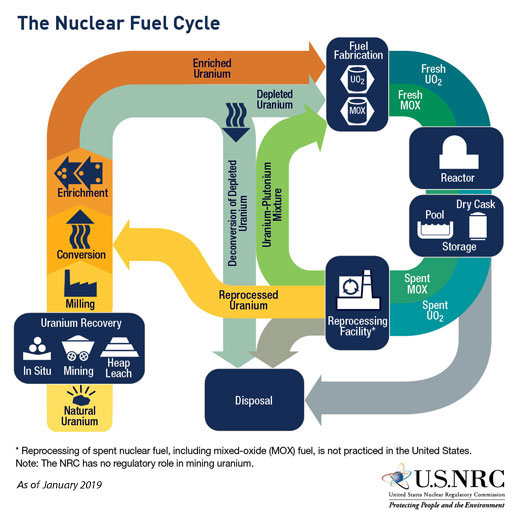
\includegraphics[scale=0.7]{nuclear_fuel_cycle.jpg}
    \caption{A complete view of options available for a once-through and 
    a recycling nuclear fuel cycle. Reproduced from 
    \protect\cite{us_nuclear_regulatory_commission_stages_2020}.}
    \label{fig:fuel_cycle}
\end{figure}

The \acrfull{NFC} has two primary sections: the front-end and 
the back-end. 
The front end encompasses the steps before the fuel arrives at a reactor 
and the back-end encompasses the steps after the fuel is discharged 
from the reactor \cite{rodriguez-penalonga_review_2017}. The 
front-end of the fuel cycle includes the mining, 
milling, conversion, and enrichment of uranium, as well as 
fuel fabrication. The mining step is the physical extraction of uranium 
ore from the earth's crust. Milling removes the non-uranium containing 
parts of the ore to purify the ore into yellow-cake uranium (U$_3$O$_8$).
The conversion step changes the chemical state of uranium compound 
for the next step in the fuel cycle. If enrichment is present, conversion 
changes the yellow-cake uranium to UF$_6$. If enrichment is not 
needed, then the uranium is converted to whatever chemical compound is 
needed for the fuel fabrication process. Enrichment modifies the 
relative abundance of different isotopes in the uranium, specifically 
to increase the abundance of $^{235}$U compared with $^{238}$U. Fuel 
fabrication then converts the (enriched) uranium to the chemical 
form required by the reactor(s) deployed. For \glspl{LWR}, fuel 
fabrication converts the enriched uranium into a UO$_2$ ceramic 
pellet. Other reactor designs may require that fuel fabrication 
produce a UCO \gls{TRISO} pebble, a molten salt, or a metallic fuel. 

The front-end of 
the \gls{NFC} is often independent of the back-end, but the back-end 
of the \gls{NFC} is highly dependent on the front-end and the reactor 
type because they govern the form and composition of the discharged 
\acrfull{SNF}. The back-end of the \gls{NFC} encompasses the 
processes and activities performed after fuel is discharged from 
a reactor. Steps commonly includes in the back-end of the \gls{NFC} 
include storage of \gls{UNF}, reprocessing, and final disposal of 
\gls{UNF}. 
The back-end of the fuel cycle can also vary, primarily based on if used 
fuel is reprocessed before final disposal. Whether or not reprocessing is 
included in determines the name for the fuel cycle: a once-through
fuel cycle if it is not includes and a recycling, twice-through, 
or closed fuel cycle if it is \cite{tsoulfanidis_nuclear_2013}. 

\subsection{Once-through fuel cycle}
A once-through fuel cycle is characterized by \gls{UNF} disposal
after discharge from a reactor, and a lack of the 
\gls{UNF} undergoing any chemical processes 
or treatments before disposal \cite{rodriguez-penalonga_review_2017}. 
The gray line from 
the storage to disposal in Figure \ref{fig:fuel_cycle} represents 
the back-end of a once-through fuel cycle. This fuel cycle does 
not include any of the material flows from the ``Reprocessing Facility'' 
in Figure \ref{fig:fuel_cycle}.
This is the fuel cycle option currently employed in the 
United States. 

Once-through \glspl{NFC} use interim storage and final disposal schemes
such as \textit{in situ} pools, dry cas storage, and geological 
repository \cite{rodriguez-penalonga_review_2017}. \gls{UNF} storage in 
an \textit{in situ} storage pool can last between 3-10 years after 
reactor discharge \cite{rodriguez-penalonga_review_2017}
and provides active cooling. Dry cask storage can be located 
on-site or at a centralized location and provides passive 
cooling to the \gls{UNF} after active cooling in a pool. 
Final disposal in a geologic repository, is the ultimate disposal 
of \gls{UNF} and 
is needed in both a once-through and recycling fuel cycle. The 
US has currently identified Yucca Mountain as a geologic repository 
site, but the site is currently not operating.  

\subsection{Recycling fuel cycle}
A recycling fuel cycle is characterized by \gls{UNF} undergoing chemical 
processes to separate out uranium, plutonium, and other 
actinides from the fuel for subsequent use in a reactor
 \cite{rodriguez-penalonga_review_2017}. 
Reuse of \gls{UNF} is possible because the metal in the fuel 
consists of 95-97\% uranium and 
plutonium \cite{rodriguez-penalonga_review_2017}, which can fission and 
produce energy in a nuclear reactor. The reuse of \gls{UNF} in 
reactors is shown by the arrows from the ``Reprocessing Facility''
node in Figure \ref{fig:fuel_cycle}. 
There are two types of recycling fuel cycle options: a limited 
recycle scheme and a continuous recycle scheme \cite{wigeland_nuclear_2014}. 
A limited recycling scheme involves fuel being reprocessed and burned in 
a reactor for a finite number of times before final disposal. This
fuel cycle scheme is sometimes referred to as a ``modified open cycle''
because of the disposal of both \gls{UNF} and \gls{HLW}
\cite{wigeland_identification_2011}. A continuous 
recycle scheme, sometimes referred to as a ``full recycle'' fuel 
cycle scheme, involves actinides from \gls{UNF} being repeatedly reprocessed 
and burned in a reactor. Disposal in this fuel cycle only includes 
fission products 
and no \gls{UNF} \cite{wigeland_identification_2011}. The difference 
in the number of times actinides and \gls{UNF} are reprocessed in each 
recycling scheme leads to differences in the amount of new resources 
(uranium) that must be acquired and the amount of material 
sent for final disposal in a repository. 

There are two primary methods to reprocess \gls{UNF}: aqueous reprocessing 
and pyroprocessing. Aqueous reprocessing relies on redox reactions of 
select actinides (typically uranium and plutonium) to move the 
actinides from an aqueous phase to an organic phase, while the non-desired 
materials in the \gls{UNF} remain in the aqueous phase \cite{rodriguez-penalonga_review_2017}. 
There 
are a variety of methods to perform aqueous reprocessing, with each method 
removing different combinations of elements from the \gls{UNF}, but the primary 
method is the PUREX process. The separated uranium and plutonium from 
aqueous reprocessing are then fabricated into \gls{MOX} fuel for use in 
a thermal-spectrum reactor. \gls{MOX} fuel can go through a limited number 
passes in a thermal reactor before disposal \cite{rodriguez-penalonga_review_2017}.
Pyroprocessing uses electric potentials to 
pull actinides (uranium and 
\glspl{TRU}) onto a cathode from a molten salt bath, while the fission products
remain in the molten salt bath or on the anode. The 
separated U/\gls{TRU} material from pyroprocessing can then be fabricated 
into metallic fuel for use in a fast-spectrum reactor. 
The \gls{UNF} from 
the fast reactor can be reprocessed multiple times and continuously put back 
into a reactor. Although this technique 
has a smaller separation factor than aqueous reprocessing, fast-spectrum 
reactors are less sensitive to impurities in the fuel and can readily use 
fuel fabricated after pyroprocessing \cite{rodriguez-penalonga_review_2017}.
Aqueous reprocessing is commercially available, and used in 
France, but pyroprocessing is not commercially available 
\cite{rodriguez-penalonga_review_2017,noauthor_status_2021}. The
type of reprocessing is more dependent on the reactor designs 
used in the fuel cycle than the fuel cycle option. For example, 
pyroprocessing is more appropriate in fuel cycles that use metallic 
fuel, because the electrorefining step requires the \gls{UNF} to 
be in a metallic form. 

Reprocessing \gls{UNF} improves resource utilization, compared 
with a once-through fuel cycle. One estimate reports that uranium ore
requirements would decrease by 25\% annually if \gls{UNF} is reprocessed 
to create \gls{MOX} fuel for \glspl{LWR} \cite{widder_benefits_2010}. 
Although this decrease in uranium ore requirements may improve the 
sustainability of the nuclear fuel cycle, current estimates of uranium 
reserves are expected to last for another 50-100 years 
\cite{widder_benefits_2010}. Therefore, reducing natural uranium usage  
is only of concern 
if there is an increase in the price of uranium ore. Another known benefit 
of reprocessing is the reduction in the volume and radioactivity of 
waste sent to a final repository. Reprocessing can reduce the waste 
volume by a factor of four \cite{widder_benefits_2010}, 
reducing the capacity of a repository required to store all the 
waste.
The radioactivity of the disposed waste decreases to about 10\% of the 
initial amount \cite{rodriguez-penalonga_review_2017} when employing 
recycling. Recycling \gls{UNF} reduces the concentration of actinides 
that are disposed of, which are the primary contributor to the long-term 
radioactivity of waste. 

Despite these benefits, recycling has known disadvantages compared to 
a once-through fuel cycle.
The amount of \gls{LLW} generated greatly increases by using 
reprocessing \cite{widder_benefits_2010}. The \gls{LLW} generated 
from reprocessing includes any solvents or materials used for the process 
and must be disposed of in accordance with regulations, but not 
necessarily in a deep geologic repository.
Pyroprocessing reduces the amount of \gls{LLW} compared with 
a once-through fuel cycle more than aqueous reprocessing because
the molten salt bath used in pyroprocessing can be cleaned 
and re-used. The \gls{LLW} generated demonstrates how the reprocessing 
technology employed affects the performance of the fuel cycle. 
Another disadvantage of reprocessing is the increased proliferation 
risk. Aqueous reprocessing creates a material stream of 
pure plutonium \cite{widder_benefits_2010}, which introduces 
concerns of material diversion to 
create a nuclear weapon. This concern led to the development of new 
methods to reprocess \gls{UNF}, such as the NUEX and COEX reprocessing 
methods, which do not create a plutonium material stream 
\cite{widder_benefits_2010}. 
Pyroprocessing has a reduced proliferation risk compared with 
aqueous reprocessing
because a plutonium material stream is never created. The extracted 
plutonium is always mixed with uranium and other \gls{TRU} material 
\cite{noauthor_status_2021}.
Additionally, reprocessing \gls{UNF} is expected to cost more than 
using a once-through fuel cycle \cite{rodriguez-penalonga_review_2017,widder_benefits_2010}. 
The estimated 
\gls{LCOE} are \$30-75/MWh for a once-through fuel cycle, with an 
average of about \$47/MWh, and \$35-81/MWh for a fuel 
cycle with reprocessing, with an average of about \$52/MWh 
\cite{widder_benefits_2010}. The ranges in the \gls{LCOE} come from 
differences in assumptions in determining the costs. Based on these 
estimates, there is no current economic incentive to reprocess and recycle 
\gls{UNF}

Each reprocessing method has advantages and disadvantages. 
A comparison of fuel cycle options for the Republic of Korea 
showed that a fuel cycle with pyroprocessing and \glspl{SFR} required less natural 
uranium than a once-through fuel cycle or a closed 
fuel cycle using aqueous reprocessing 
and \glspl{PWR} to produce the same amount of energy 
\cite{park_comparative_2011}. Both methods of reprocessing  
reduced the amount of \gls{UNF} for disposal,
but using pyroprocessing with a fast reactor produced no \gls{UNF} for 
disposal. The separated material from 
pyroprocessing that cannot be recycled in a reactor is assumed to be 
disposed of as \gls{LLW} in the analysis. This assumption 
holds true, such that this waste stream is no longer 
\gls{UNF}, but the material would likely be disposed of 
as \gls{HLW} in the US.
One disadvantage of reprocessing 
identified by Park et al. \cite{park_comparative_2011} is the 
increase in \gls{LLW} produced 
when using aqueous reprocessing and 
thermal reactors. This result is consistent with the analysis 
by \cite{widder_benefits_2010}, which showed a decrease in \gls{LLW} 
mass when using a fuel cycle with pyroprocessing and fast reactors, 
compared with a once-through fuel cycle \cite{park_comparative_2011}. 

\section{Uranium enrichment}
In the \gls{NFC}, enrichment increases the relative abundance of 
$^{235}$U compared with $^{238}$U in the fuel, increasing
the relative abundance of fissile material required
for operating most reactor designs. There are multiple technologies and processes 
that can enrich uranium: gaseous diffusion, calutrons, gaseous centrifuges, 
and laser separation technologies. The US currently employs gaseous 
centrifuges to enrich uranium for commercial supplies. Gaseous centrifuges 
are currently used at the Urenco site in New Mexico 
\cite{us_nuclear_regulatory_commission_louisiana_2022} and planned for the 
Centrus facility in Piketon, Ohio 
\cite{us_nuclear_regulatory_commission_centrus_2021}. Gaseous centrifuges 
are rotating canisters, 
relying on the speed of the rotation to move heavier 
materials to the outside of the canister. Because of this preferential 
movement, a greater concentration of the lighter material ($^{235}$U) 
accumulates near the middle of the canister \cite{villani_uranium_1979}. 
To ensure that only the mass difference in the uranium isotopes causes 
this preferential separation, the uranium is sequestered in UF$_6$ gas, because 
fluorine only has one naturally occurring isotope and thus 
does not contribute to any mass differences between 
molecules of $^{235}$UF$_6$ and $^{238}$UF$_6$. 

Multiple quantities govern the capacity of an enrichment facility 
\cite{tsoulfanidis_nuclear_2013}, defined in Table \ref{tab:enrichment_variables}.
The enrichment facility separates the feed material (typically
natural uranium) into product and tails streams. The product stream is 
material at the desired enrichment level and the tails stream 
in material at enrichment levels lower than that of the 
feed material. Each of these material streams have a 
defined assay or weight fraction of $^{235}$U. The \acrfull{SWU} capacity 
is the physical work required to put into the system to provide the 
separation needed to meet the product stream demand. It is also related 
to the amount of energy the facility 
requires \cite{tsoulfanidis_nuclear_2013}. 
Each of the quantities in Table \ref{tab:enrichment_variables}
can be related using the following equations:
\begin{subequations}
    \begin{equation}
        F = P + T
    \end{equation}
    \begin{equation}
        x_fF = x_pP + x_tT
        \label{eq:enrichment_assasys}
    \end{equation}
    \begin{equation}
        SWU = \left[P*V(x_p) +T*V(x_t) - F*V(x_f)\right]*t
        \label{eq:swu}
    \end{equation}
    \text{in which:}
    \begin{equation}
        V(x_i) = (2x_i - 1)*\ln\left(\frac{x_i}{1-x_i}\right)
        \label{eq:sep_potential}
    \end{equation}
    \label{eq:enrichment}
\end{subequations}

\begin{table}[ht]
    \centering
    \caption{Definitions for variables used to describe throughput and 
    capacity for an enrichment facility.}
    \label{tab:enrichment_variables}
    \begin{tabular}{c c c}
        \hline
        Variable & Description & Units\\\hline
        F & Mass of feed material per unit time & kg\\
        P & Mass of product material per unit time & kg \\
        T & Mass of tails material per unit time & kg\\
        x$_f$ & weight fraction of $^{235}$U in the feed stream & -\\
        x$_p$ & weight fraction of $^{235}$U in the product stream & - \\
        x$_t$ & weight fraction of $^{235}$U in the tails stream & - \\
        \gls{SWU} & the physical work required to separate the isotopes & kg-SWU\\
        t & time step & d\\
        V & Separation Potential & - \\
        x$_i$ & weight fraction of $^{235}$U in the $i$ stream & - \\
        \hline
    \end{tabular}
\end{table}

The subequations comprising Eq. \ref{eq:enrichment} show that as the desired 
enrichment level 
of the product feed increases, the feed mass must also increase, assuming everything 
else is held constant. The equations also show that as the desired 
product 
enrichment level increases, the amount of \gls{SWU} capacity needed also increases. 
However, if the product mass decreases, then the required \gls{SWU} capacity 
also decreases. Therefore, changes to the product enrichment level and mass 
throughput have similar effects on the amount of feed material and required 
\gls{SWU} capacity. Opposing changes to both quantities 
(i.e., an increase in one and a decrease in the other) will not lead to a clear 
expectation for the change in feed material of the \gls{SWU} capacity. 
The effect on these variables will depend on the magnitude of the changes.

The separation needed to enrich uranium cannot be performed 
in a single 
separation step because of the small separation efficiency of gas centrifuges. 
Therefore, centrifuges at a facility are placed into  
cascades, as shown in Figure \ref{fig:cascade}. Each cascade is designed with 
multiple separation stages in series, with multiple centrifuge units in 
parallel comprising each stage \cite{villani_uranium_1979}. Each stage 
outputs a product enriched to a certain amount (less than the final product 
of the cascade), then the product from one 
stage becomes the feed material for the next stage in the cascade to produce 
a greater enrichment level. The tails material from each 
stage is combined with feed material for the previous stage, to help strip 
out any $^{235}$U that is left in the tails. Figure 
\ref{fig:cascade} does not show the use of tails from each stage 
as feed for the previous step. Using the tails in the 
previous stage develops the cascade into a counter-current cascade 
\cite{villani_uranium_1979} and helps to improve the efficiency of the entire cascade. 
Depending on the mass of product material needed, an enrichment 
facility may have multiple cascades, with each cascade housing multiple 
centrifuges. 
Changing the product stream assay (the $^{235}$U weight fraction)
requires a change in the cascade configuration of 
a facility, even if the required \gls{SWU} capacity is the same. Therefore, 
understanding the product stream assay, \gls{SWU} capacity needed, and the 
amount of product needed aids in designing facilities to meet potential 
demand of \gls{HALEU}.

\begin{figure}
    \centering
    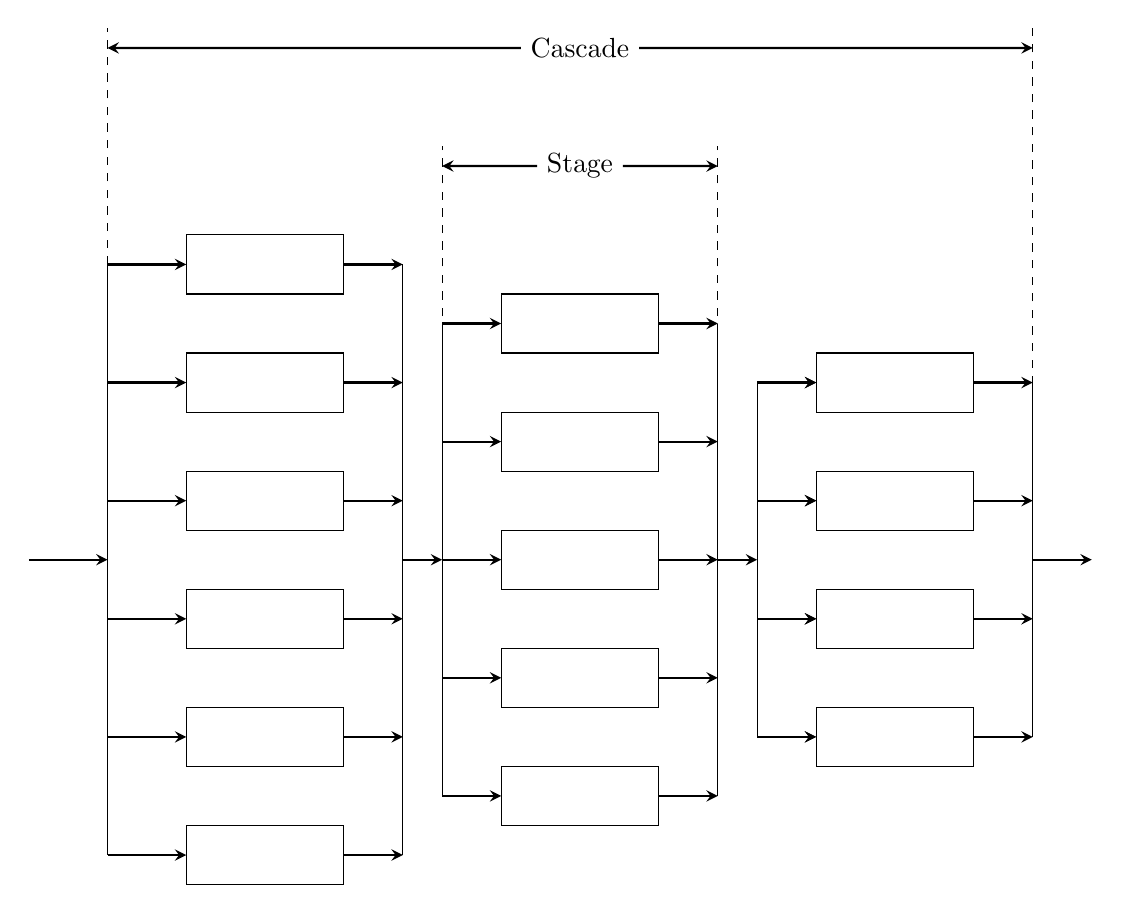
\begin{tikzpicture}[node distance=1.5cm]
        \node (C1) [centrifuge] {};
        \node (C2) [centrifuge, below of=C1] {};
        \node (C3) [centrifuge, below of=C2] {};
        \node (C4) [centrifuge, below of=C3] {};
        \node (C5) [centrifuge, below of=C4] {};
        \node (C6) [centrifuge, below of=C5] {};
        \node (C7) [centrifuge, right of=C1, xshift=2.5cm, yshift=-0.75cm] {};
        \node (C8) [centrifuge, below of=C7] {};
        \node (C9) [centrifuge, below of=C8] {};
        \node (C10) [centrifuge, below of=C9] {};
        \node (C11) [centrifuge, below of=C10] {};
        \node (C12) [centrifuge, right of=C7, xshift=2.5cm, yshift=-0.75cm] {};
        \node (C13) [centrifuge, below of=C12] {};
        \node (C14) [centrifuge, below of=C13] {};
        \node (C15) [centrifuge, below of=C14] {};
        \node (label1) [draw=none, fill=none, above of=C7, yshift=2cm] {Cascade};
        \node (label2) [draw=none, fill=none, below of=label1] {Stage};

        
        \draw [arrow] (-3,-3.75)--(-2,-3.75);
        \draw (-2,0) -- (-2,-7.5);
        \draw [arrow] (-2,0) -- (-1,0);
        \draw [arrow] (-2,-1.5) -- (-1,-1.5);
        \draw [arrow] (-2,-3) -- (-1,-3);
        \draw [arrow] (-2,-4.5) -- (-1,-4.5);
        \draw [arrow] (-2,-6) -- (-1,-6);
        \draw [arrow] (-2,-7.5) -- (-1,-7.5);
        \draw [arrow] (1,0) -- (1.75,0);
        \draw [arrow] (1,-1.5) -- (1.75,-1.5);
        \draw [arrow] (1,-3) -- (1.75,-3);
        \draw [arrow] (1,-4.5) -- (1.75,-4.5);
        \draw [arrow] (1,-6) -- (1.75,-6);
        \draw [arrow] (1,-7.5) -- (1.75,-7.5);
        \draw (1.75,0) -- (1.75,-7.5);
        \draw [arrow] (1.75,-3.75)--(2.25,-3.75);
        \draw (2.25,-0.75) -- (2.25,-6.75);
        \draw [arrow] (2.25,-0.75) -- (3,-0.75);
        \draw [arrow] (2.25,-2.25) -- (3,-2.25);
        \draw [arrow] (2.25,-3.75) -- (3,-3.75);
        \draw [arrow] (2.25,-5.25) -- (3,-5.25);
        \draw [arrow] (2.25,-6.75) -- (3,-6.75);
        \draw [arrow] (5,-0.75) -- (5.75,-0.75);
        \draw [arrow] (5,-2.25) -- (5.75,-2.25);
        \draw [arrow] (5,-3.75) -- (5.75,-3.75);
        \draw [arrow] (5,-5.25) -- (5.75,-5.25);
        \draw [arrow] (5,-6.75) -- (5.75,-6.75);
        \draw (5.75,-0.75) -- (5.75,-6.75);
        \draw [arrow] (5.75,-3.75)--(6.25,-3.75);
        \draw (6.25,-1.5) -- (6.25,-6);
        \draw [arrow] (6.25,-1.5) -- (7,-1.5);
        \draw [arrow] (6.25,-3) -- (7,-3);
        \draw [arrow] (6.25,-4.5) -- (7,-4.5);
        \draw [arrow] (6.25,-6) -- (7,-6);
        \draw [arrow] (6.25,-1.5) -- (7,-1.5);
        \draw [arrow] (6.25,-3) -- (7,-3);
        \draw [arrow] (6.25,-4.5) -- (7,-4.5);
        \draw [arrow] (6.25,-6) -- (7,-6);
        \draw (9.75,-1.5) -- (9.75,-6);
        \draw [arrow] (9, -1.5) -- (9.75,-1.5);
        \draw [arrow] (9, -3) -- (9.75,-3);
        \draw [arrow] (9, -4.5) -- (9.75,-4.5);
        \draw [arrow] (9, -6) -- (9.75,-6);
        \draw [arrow] (9.75,-3.75)--(10.5,-3.75);

        \draw [dashed] (-2,0) -- (-2,3);
        \draw [arrow] (label1) -- (-2,2.75);
        \draw [dashed] (9.75,-3) -- (9.75,3);
        \draw [arrow] (label1) -- (9.75,2.75);
        \draw [dashed] (2.25,-1.5) -- (2.25,1.5);
        \draw [arrow] (label2) -- (2.25, 1.25);
        \draw [dashed] (5.75,-1.5) -- (5.75,1.5);
        \draw [arrow] (label2) -- (5.75, 1.25);
        \end{tikzpicture}
    \caption{Diagram of material flow through an enrichment facility 
    cascade. The lines and arrows shown are the product stream from each unit, and the 
    tails stream is not shown. Each box represents a single centrifuge, or 
    unit. How the units comprise a stage, each vertical column,
    and the cascade, the entire configuration, are identified. 
    Figure recreated from \protect\cite{villani_uranium_1979}.}
    \label{fig:cascade}
\end{figure}

The design parameters for a cascade are optimized based on the separation 
factor 
achieved in the centrifuges, the UF$_6$ flow rate, and the material assays. 
The required product assay and the separation factor of each stage govern 
the number of stages required in a cascade \cite{whitaker_uranium_2019}. 
Therefore, to achieve a higher product assay either more stages 
need to be added or each stage needs to achieve a greater separation
factor. The product flow rate governs the number of centrifuges in 
each stage \cite{whitaker_uranium_2019}. As the flow rate increases, 
so do the number of centrifuges per stage. 


%%%%%%%%%%%%%%%%%%%%%%%%%%%%%%%%%%%%%%%%%%%%%%%%%%%%%%%%%%%%%%%%%%%
%
%
%
%%%%%%%%%%%%%%%%%%%%%%%%%%%%%%%%%%%%%%%%%%%%%%%%%%%%%%%%%%%%%%%%%%%
\section{Fuel cycle simulators}
\gls{NFC} simulators are computational tools to model the flow of materials
and the commissioning and decommissioning of facilities for a fuel 
cycle. \gls{NFC} simulators can evaluate the transition between fuel cycle 
options (e.g., from a once-through to a recycling fuel cycle), the 
performance of one fuel cycle with a growth in the demand of nuclear power, 
and the effect of perturbations on the material and facility 
requirements for a fuel cycle \cite{piet_dynamic_2011}. 
\gls{NFC} simulators include multiple functionalities and 
capabilities: material flow tracking, facility deployment and 
retirement, timing, facility capacities, and external fissile material 
sources (e.g., mines) \cite{brown_identification_2016}.
each of the features listed here are considered ``foundational 
capabilities'' by Brown et al. 
\cite{brown_identification_2016}. Each of these features can then be 
expanded upon through ``integral'' or ``exemplary'' features to expand the 
foundational capabilities. Examples of integral
features include strategic deployment of facilities to meet a specified 
material demand or material prioritization. Examples of exemplary
features include modeling radioactive decay of materials or calculations 
of fuel depletion in a reactor \cite{brown_identification_2016}. 

A variety of fuel cycle simulators have been developed, often to focus on 
specific areas of the \gls{NFC} \cite{huff_next_2010}. Some of the 
\gls{NFC} simulators developed include
\gls{DYMOND} \cite{feng_sensitivity_2020,feng_standardized_2016}, 
\gls{VISION} \cite{yacout_visionverifiable_2006}, ORION 
\cite{gregg_analysis_2012}, COSI6 \cite{coquelet-pascal_cosi6:_2015}, and
\gls{NFCSim} \cite{schneider_nfcsim:_2005}. 
Another \gls{NFC} simulator is \Cyclus, an open-source, agent-based 
\gls{NFC} simulator \cite{huff_fundamental_2016}. The next section 
describes \Cyclus more in-depth because it is the simulator chosen for this 
work. 
\gls{DYMOND} is a fuel cycle simulator developed by \gls{ANL} initially for 
the Gen IV Fuel Cycle Crosscut Group. This simulator combines 
multiple modeling paradigms, including system dynamics, discrete events, and
agent-based modeling \cite{feng_standardized_2016,feng_sensitivity_2020}.
\gls{DYMOND} accepts inputs of reactor and fuel characteristics, fuel cycle 
facility properties, the facilities that use each fuel type, and an 
energy demand to output the reactor fleet composition \cite{feng_standardized_2016}.
\gls{VISION} was developed primarily to meet the program objectives of the 
\gls{AFCI} and is based on \gls{DYMOND} \cite{yacout_visionverifiable_2006}.
\gls{VISION} was initially developed to be US-focused, but has been modified to 
be more generalized in its capabilities \cite{feng_standardized_2016}.
\gls{VISION} dynamically models the mass flow of material through the 
entire fuel cycle and calculates metrics based on the \gls{AFCI} program 
objectives. New functionalities added to \gls{VISION}, compared with \gls{DYMOND}, 
include estimating economic costs and modeling isotope decay. 
\gls{VISION} has multiple 
modules to model the mass flow, calculate metrics, perform control, or 
integration. 
Both \gls{DYMOND} and \gls{VISION} model the fuel cycle at a fleet level, 
instead of a facility level \cite{feng_standardized_2016}.  
The UK National Nuclear Laboratory developed ORION, which tracks up to 
2500 nuclides as they 
move through a nuclear fuel cycle \cite{gregg_analysis_2012}. ORION models
facilities as individual objects, it models
the decay and irradiation of the tracked nuclides 
\cite{feng_standardized_2016}. COSI6 was developed by \gls{CEA} to 
study different evolutions of reactors and fuel cycles and 
provide technical information to decision makers \cite{coquelet-pascal_cosi6:_2015}. 
COSI6 simulates a fuel 
cycle in a chronological order based on user-provided inputs, and does 
not provide any decision making. \gls{NFCSim} was developed by \gls{LANL}
to address contemporary gaps in the ability of fuel cycle simulators 
to model transition scenarios or time-dependent information of 
sensitive material locations \cite{schneider_nfcsim:_2005}. 
\gls{NFCSim} applies an object-oriented 
philosophy to represent each element of a fuel cycle model. Objects 
are grouped into classes, with classes grouped together to form 
superclasses. 

\subsection{\Cyclus}
\Cyclus is a dynamic, open source agent-based fuel cycle simulator. Built 
in C++, \Cyclus uses only open source and freely available libraries to 
provide full access to all users and developers. The 
\Cyclus architecture treats materials and facilities independently, similar 
to ORION, and allows 
for variable fidelity levels \cite{huff_fundamental_2016}. These attributes
of \Cyclus allow for the software to model any fuel cycle scenario.

\Cyclus uses the notion of an \textit{agent} to represent different 
components in the simulated fuel cycle. Agents are 
defined using the \Cyclus \gls{API}, which allows users 
to develop their own suite of agent libraries and use them within \Cyclus. 
The \gls{API} anticipates the structure on information about a given 
library 
required by the core \Cyclus kernel, facilitating 
information sharing between the library and the \Cyclus framework. 
This framework 
also allows for flexibility in licensing and distribution of the 
user-developed libraries. Libraries are loaded without changes to the \Cyclus 
kernel and without unwanted transfer of sensitive information, allowing 
agent library development with export controlled 
software while still allowing \Cyclus to be open-source.

The agent-based modeling paradigm employed by \Cyclus allows agent level 
modeling, as opposed to system level modeling. This paradigm allows different 
fuel cycle facilities, such as a reactor and a fuel fabrication plant, to 
be defined independently but still interact with each other in the 
simulation. There are three main groups of agents within the \Cyclus 
architecture: facilities, institutions, and regions. The agent types
are related using a parent-child hierarchy: regions are
parents of institutions, and institutions are parents of facilities.
Facilities are 
the individual units in the fuel cycle that implement technologies, 
such as a fuel fabrication facility or a uranium mine. Institutions 
manage the facilities, similar to how a company manages facilities, 
and are responsible for the deployment of facilities. 
Regions provide geographic 
and political context for the institutions and regions and can be thought 
of as similar to individual nations. 

The \Cycamore agent library provides a variety of libraries that can be 
dynamically loaded into \Cyclus for use in a simulation 
\cite{huff_fundamental_2016,carlsen_cycamore_2014}. These libraries 
include multiple facilities, two institutions, and one region as of 
\Cycamore 1.3 \cite{huff_fundamental_2016}. The two institutions 
(the \texttt{DeployInst} and \texttt{ManagerInst}) interact 
with the region (the \texttt{GrowthRegion}) to deploy 
facilities as needed to meet a commodity demand specified by the region. 
The \texttt{DeployInst} manually defines the number of each 
facility to be deployed at each time step. These facilities 
registered with the \texttt{GrowthRegion} for their 
contribution to the demand and are decommissioned at the end of their 
lifetime. The 
\texttt{ManagerInst} calculates the number of each facility 
type to deploy to meet the demand given by the \texttt{GrowthRegion}, 
based on what is not met through facilities deployed by other institutions 
in the region.  

In \Cyclus, agents trade materials through the \gls{DRE} 
\cite{gidden_agent-based_2015,huff_fundamental_2016}. The \gls{DRE} defines the 
supply-demand communication framework and treats facilities as black boxes
so the solution strategy is agnostic to the resource types being exchanged. 
The \gls{DRE} is a novel concept and unique to \Cyclus. It provides a 
flexible architecture to support supply-demand modeling and dynamic 
material flows between facilities \cite{huff_fundamental_2016}. 
There are three steps in the \gls{DRE}: information gathering, resource 
exchanges, and trade execution \cite{gidden_agent-based_2015}. 
During the information gathering 
phase facilities that need materials state their demand for a given 
material (e.g., a reactor stating a demand for fuel), referred to 
as requests. Requests 
from a facility can be more than what is actually required (e.g. a reactor
requesting extra fuel assemblies just in case one breaks mid-cycle). Additionally, 
facilities can state mutual requests, or state requests for materials in 
which either of the materials would meet the demand (e.g., a reactor 
requesting UOX and MOX fuel but only needing one to meet their request), with 
a preference defined for each material. Requests for materials can have 
constraints attached, such as quantity limits or if the request is 
\textit{exclusive}. Exclusive requests mean that it must be met fully 
from a single response to the request (or bid), as opposed to being met 
through multiple small 
bids. Then facilities that produce materials also state the amount of a 
material they have to trade away (e.g., a fuel fabrication plant stating 
that they have 3 fuel assemblies), as the or 
bids. Using the information of the material requests and the bids, 
the \gls{DRE} creates an exchange graph. The exchange graph is a 
bipartite network \cite{gidden_agent-based_2015}
with nodes for the requests and the responses to the requests. 

Once the exchange graph is created, the requesting facilities can apply 
preferences to possible each potential bid based on the facility 
making the bid \cite{huff_fundamental_2016}. Preferences can be based on 
the agent making the bid, the bidding agent's institution, or 
the bidding agent's 
region. For example, a reactor agent can prefer to receive fuel 
assemblies from agent(s) that belong to a specific institution (mimicking but not 
fully enforcing contracts between companies), or agents in a specific region 
(mimicking international trade agreements). The addition of preferences of 
potential bids allows the \gls{DRE} to more closely mimic supply chain 
dynamics within a fuel cycle. 
A solution is found to the exchange graph by matching requests with 
responses. A feature of \Cyclus is that it is possible for 
requests to be unmet if there is not enough material in the responses 
to fully meet the bid. To account for this 
capability, unconstrained false nodes are defined in the exchange graph
to ensure a feasible solution is possible \cite{gidden_methodology_2016}.
A solution to the exchange graph is found using a simulation-based 
heuristic or a mathematical program \cite{gidden_agent-based_2015}.
Mathematical models to solve the exchange graph include \gls{MILP} and 
\gls{LP}, with \gls{MILP} required to solve the exchange graph if 
any of the requests are denoted as exclusive \cite{huff_fundamental_2016}.
Once a solution is found to the exchange graph, the materials are 
traded between the matched facilities in the trade execution phase.  
In the trade execution phase, the materials are traded between the 
facilities matched between the requests and bids. 

Similar to many of the other fuel cycle simulators developed, material 
compositions in \Cyclus are defined using recipes. Recipes are 
typically defined as stagnant compositions at the beginning of 
a simulation. However, there are instances in which fuel compositions 
need to be dynamic during a simulation, such as when accounting for fuel 
depletion. The next section discussed how different fuel 
cycle simulators address fuel depletion. 

\subsection{Fuel depletion} \label{sec:depletion}
Fuel depletion is an important component of fuel cycle simulations 
because the composition of used fuel affects the decay heat, 
amount of fissile material present, and the volume of the used 
fuel. Each of these fuel properties affects transportation of the 
\gls{UNF}, 
repository storage limits, and how much material is available for 
reprocessing and recycling. Therefore, fuel cycle simulators must 
have a way to account for fuel depletion. 

One possible way to account for fuel depletion is pre-define  
compositions of used fuel and update the composition of fuel 
materials when 
they are discharged from a reactor. This methodology is used 
in VISION \cite{yacout_vision_2006}, the \Cycamore \texttt{Reactor} 
archetype \Cyclus \cite{carlsen_cycamore_2014},
and is available through ORION \cite{sunny_transition_2015}. To 
use this method the 
used fuel compositions must be known \textit{a priori}, with used fuel 
compositions typically obtained by using another program 
to model depletion before modeling the fuel cycle. 
This method of accounting for fuel depletion provides a fast and 
simple way to model a fuel cycle. Although it has been used to 
model closed fuel cycles \cite{bae_standardized_2019,djokic_application_2015},
it is most appropriate for once through fuel cycles 
\cite{sunny_transition_2015} because the same 
compositions for fresh fuel are loaded into a reactor at each 
refueling, which means that the used fuel compositions do not vary 
greatly between discharged batches. 

Brown et al. consider dynamic modeling of fuel depletion, or 
modeling depletion during a fuel cycle simulation, to be an 
``exemplary'' quality 
of a fuel cycle simulator \cite{brown_identification_2016},
and is available in different simulators. Dynamic depletion 
modeling allows a fuel cycle simulator to more accurately model  
the effects of depletion on fuel compositions in a fuel cycle. Some of the 
fuel cycle simulators that have dynamic fuel depletion capabilities 
are ORION \cite{feng_standardized_2016}, \gls{DYMOND} 
\cite{richards_application_2021}, and \gls{NFCSim} \cite{schneider_nfcsim:_2005}.
ORION allows 
users to define material compositions using recipes or have the 
program model decay and depletion of the material \cite{sunny_transition_2015}. ORION 
has some built-in reactor-specific cross sections for modeling 
depletion during a fuel cycle simulation, or users can generate 
and provide their own cross section data customized for the reactors and fuel cycle 
they are modeling. \gls{DYMOND} models depletion through a coupling with 
ORIGEN2, a stand-alone depletion solver, using pre-generated 
reactor-specific depletion libraries \cite{richards_application_2021}.
The coupling of \gls{DYMOND} with ORIGEN2 provides dynamic updates to 
used fuel compositions, but it also allows for the code to perform 
criticality searches to determine fresh fuel compositions based on 
the used fuel compositions available. This criticality search provides 
more accurate compositions of the fresh fuel produced than using a recipe 
to define the composition because it creates a feedback mechanism 
between the fresh and used fuel compositions \cite{richards_application_2021}.
However, the increased accuracy in fuel compositions in \gls{DYMOND} comes 
at the cost of increased computational cost \cite{richards_application_2021}.
\gls{NFCSim} is coupled with \gls{LACE}, a criticality and burnup 
engine developed to couple with \gls{NFCSim} to model the 
time-dependent nature of nuclear materials in a fuel cycle simulation
\cite{schneider_nfcsim:_2005}. By providing \gls{LACE} with cross 
section libraries, it can find fluence-dependent burnups and production 
and destruction rates for actinides in the fuel materials. This 
information is then used to develop reactor-specific reactivity models 
based on the fluence as the independent variable. This coupling 
with \gls{LACE} provides a cycle-dependent way to determine 
used fuel compositions upon discharge from the reactor or at a 
later time (e.g., after initial cooling or upon entrance to a 
separations facility). 

The core kernel of \Cyclus does not provide a method to dynamically 
model depletion of fuel. However, the modular nature of \Cyclus means 
that developers can easily create archetypes that provide this 
functionality. One such archetype is \gls{CYBORG}, which is a 
reactor-style archetype that couples \Cyclus with ORIGEN 
\cite{skutnik_cyborg_2016}. \gls{CYBORG} leverages the validated 
depletion capabilities in ORIGEN to model fuel depletion during 
a fuel cycle simulation \cite{skutnik_cyborg_2016}. User-defined 
parameters (such as fresh fuel compositions, irradiation time, and 
power level) are passed to \gls{CYBORG}, which then produces a 
problem-specific cross section library. The library is then passed to 
ORIGEN to perform the depletion calculation. The depleted material 
compositions are then passed to \Cyclus to update the appropriate 
material compositions and recipes in a simulation. Use of this 
archetype requires users to have a license to use ORIGEN, as it 
is an export-controlled code, which can pose issues in a user being 
able to use this archetype. 

A third-party archetype library developed to account for fuel depletion 
is Bright-lite \cite{schneider_integrated_2016}. The Bright-lite 
library contains three different archetypes: \texttt{ReactorFacility}, 
\texttt{FuelfabFacility}, \texttt{ReprocessingFacility}. This archetype library 
models depletion by determining fresh and used fuel compositions
based on burnup, criticality, and transmutations matrix curves. 
Bright-lite has two operation modes: forward mode and blending 
mode \cite{schneider_integrated_2016}. In forward mode, Bright-lite 
reads in a defined fuel composition and depletes based on the neutron 
fluence through the material and a target (i.e. \keff=1). In 
blending mode, Bright-lite connects the ReactorFacility and 
\texttt{FuelfabFacility} to mix multiple material streams to create a single 
stream that meets a specific target: burnup-criticality or burnup-conversion
ratio. This archetype library can be used for modeling multiple reactor 
designs and multiple fuel forms, but requires different cross 
section libraries for each reactor and fuel type. Bright-lite comes 
with pre-defined libraries or a user may supply their own 
library that can be interpolated by Bright-lite. There is little 
published use of this archetype library in the current literature, 
suggesting that there are significant barriers to its use or that 
other archetypes are sufficient to meet the performance of this 
archetype library. 

A third archetype to add dynamic depletion capabilities to \Cyclus 
is the ann\_pwr archetype \cite{bae_deep_2020}. This archetype 
attempts to strike a balance between computational cost and 
depletion accuracy by predicting the used fuel composition based on 
fuel burnup and initial enrichment using trained neural networks.
A similar depletion method was used with the \gls{CLASS} 
\gls{NFC} simulator to predict core loading and cross section data 
for a \gls{PWR} loaded with \gls{MOX} fuel \cite{leniau_neural_2015}.
The neural networks for the ann\_pwr archetype were trained 
on data in the \gls{UNFSTANDARDS} \gls{UDB} \cite{peterson_used_2013}.
Performance of this archetype is very promising, showing much faster 
compute times and reduced memory requirements than other depletion 
methods as well as greater agreement to the data in the \gls{UDB} than 
using a standard recipe composition \cite{bae_deep_2020}. However, 
this archetype is very limited in applicability for many fuel cycles. 
The neural network was trained only on data from \gls{PWR}
assemblies, so a user cannot use this archetype to model depletion 
in other reactor types. Expansion of this archetype to include 
other reactor types would require developing separate neural networks for 
each reactor design, or the develop a new network that accounts for 
reactor type as an input parameter. 

\subsection{Verification and use of fuel cycle simulators}
Verification activities of \gls{NFC} provides a comparison of the 
results from different simulators for a defined fuel cycle. 
These activities are important because each fuel cycle 
simulator uses a different methodology for defining materials 
and facilities. These activities also identify different 
modeler interpretations of the fuel cycle information, 
and how to translate that into a fuel cycle model. 
Multi-lab efforts validated some of the \gls{NFC} simulators discussed here 
(\gls{DYMOND}, \gls{VISION}, ORION, and \Cyclus)
using a no growth transition from \glspl{LWR} 
to \glspl{SFR} \cite{feng_standardized_2016,bae_standardized_2019}.
Each \gls{LWR} in the scenario provides 1000 MWe of 
electricity and each \gls{SFR} provides 333.3 MWe of electricity. The 
scenario is simple enough that a spreadsheet could calculate the results, 
which served as an analytical solution. The 
results from each \gls{NFC} simulator were compared to each other and 
to the spreadsheet solution. Any observed differences were either explained 
based on modeling implementation or resolved through changes to the 
necessary code.

The results of the verification efforts showed agreement between each 
of the codes and the spreadsheet results, but it also identified modeling 
differences. For example, \gls{VISION} and \gls{DYMOND} model continuous 
reprocessing at each time step, as opposed to the instantaneous 
reprocessing modeled by the spreadsheet \cite{feng_standardized_2016}. 
This difference led to \gls{DYMOND} reporting lower annual mass flow 
rates for the \glspl{SFR} and a small delay in the idle \gls{UNF} 
inventory modeled by \gls{VISION} compared with the spreadsheet 
solution. 
Another difference identified is that the \Cycamore Reactor 
archetype models each fuel assembly and batch as discrete material 
\cite{bae_standardized_2019}, as 
opposed to the other codes assuming continuous fuel discharge. 
This difference leads to oscillations in the \gls{UNF} discharged 
when using \Cyclus, while the other codes results do not have these 
oscillations.
However, this modeling decision in \Cyclus produced results that 
are closer to reality, because of the cyclic nature of fuel 
loading and discharge from reactors. 
Additionally, the \Cycamore Reactor archetype depletes half of the 
core of fuel upon decommissioning, while the other \gls{NFC} simulators 
deplete the entire core of fuel upon decommissioning. This 
difference affects the \gls{TRU} material inventory, and the 
methodology was 
temporarily removed to demonstrate that the different 
methodologies led to the difference in results \cite{bae_standardized_2019}.

A common use of \gls{NFC} simulators is to evaluate the performance 
of fuel cycles based on specific criteria. 
For example, work with \gls{DYMOND}, \gls{DANESS}, 
and \gls{NFCSim} evaluated how different fuel cycle options 
could reduce \gls{UNF} volume in a repository \cite{yacout_dynamic_2004}. 
This work showed how the exclusion of \glspl{TRU} from material 
sent to a repository significantly decreases the decay heat 
of material in the repository. 
\gls{NFC} simulators have also evaluated the transition between fuel cycle 
options. Dynamic simulations of fuel cycle options for the \gls{AFCI}
Campaign in 2005 demonstrate the importance of the magnitude, timing, 
and rate of deploying facilities for meeting demands of the new fuel cycle option 
\cite{piet_assessment_2011}. Furthermore, \gls{NFC} simulators are 
used to model the transition between 
different fuel cycle options or technology. Quantifying the transition 
between fuel cycle options occurs by studying metrics such as the 
energy output and resource requirements of the transition 
\cite{del_cul_advanced_2010}. 
Resource requirements can include the mass of natural uranium, enrichment 
needs, fuel irradiation, \gls{UNF}, waste production, and cost. 

The use of \gls{NFC} simulators over the 
last decade has primarily been guided by the Nuclear Fuel Cycle \gls{ES} 
from the \gls{DOE-NE} \cite{wigeland_nuclear_2014}. This project
categorized multiple fuel cycle options into 40 different \glspl{EG} 
based on characteristics such as the recycling scheme, the type of fuel 
burned, 
and the type of reactor (e.g., thermal critical reactor, fast critical reactor). 
The \glspl{EG} were compared on their performance at equilibrium on nine evaluation 
criterion, including nuclear waste management and resource utilization. The 
results of this project showed that the most benefit comes from fuel cycles 
that use continuous recycling of U/Pu with new or natural uranium in fast critical 
reactors (\gls{EG} 23), continuous recycling of U/\gls{TRU} with new or natural 
uranium in fast critical reactors (\gls{EG} 24), continuous recycling of U/Pu 
with new or natural uranium in both fast and thermal critical reactors 
(\gls{EG} 29), or continuous recycling of U/\gls{TRU} with new or natural uranium in 
both fast and critical reactors (\gls{EG} 30) \cite{wigeland_nuclear_2014}. 

Based on the results of the \gls{ES}, several efforts modeled 
the transition to these promising fuel cycle options using fuel cycle 
simulators \cite{sunny_transition_2015,djokic_application_2015,feng_standardized_2016,bae_standardized_2019,littell_development_2016}. 
Researchers used ORION to model the transition from a 
once-through fuel cycle option using enriched uranium in thermal critical 
reactors to a closed fuel cycle with U/Pu recycling in fast 
critical reactors (\gls{EG} 01 to \gls{EG} 23) \cite{sunny_transition_2015}.
This work 
demonstrated the importance of new \glspl{LWR} and license 
extensions of existing reactors for this transition. 

Djokic et al. used \Cyclus to model the transition from \gls{EG} 01 to \gls{EG} 
23 assuming a 1\% growth in power demand 
\cite{djokic_application_2015}. The results from \Cyclus were compared 
to the results from modeling the same transition scenario with \gls{DYMOND}. 
The power generated, reactor entry 
time, and reactor exit time for the \Cyclus simulation qualitatively 
matches well with the results of the \gls{DYMOND} simulation, but the power 
demand growth could match better to the target 1\% by slightly modifying 
the \gls{SFR} deployment \cite{djokic_application_2015}. Littell 
\cite{littell_development_2016}
also modeled the \gls{EG} 01 to \gls{EG} 23 transition in \Cyclus. 
This work included constraints such as restricting the mass of separated 
plutonium to less than 100 MT, not allowing reprocessing to begin until 
at least 2050, and allowing up to 5\% surplus or deficit in the energy 
from compared with the demand. This work found that the separated 
plutonium constraint could be met, except when reprocessing first 
begins because of the accumulation of \gls{UNF} before 
reprocessing begins \cite{littell_development_2016}. 

%%%%%%%%%%%%%%%%%%%%%%%%%%%%%%%%%%%%%%%%%%%%%%%%%%%%%%%%%%%%%%%%%%%%%%%
%
%
%
%%%%%%%%%%%%%%%%%%%%%%%%%%%%%%%%%%%%%%%%%%%%%%%%%%%%%%%%%%%%%%%%%%%%%%%
\section{Sensitivity analysis and optimization}
Sensitivity analysis identifies and quantifies how each input parameter 
of a model affects output metrics \cite{thiolliere_methodology_2018}. 
Sensitivity analysis is useful in fuel cycle modeling because of the 
multiple sources of uncertainty in 
modeling the nuclear fuel cycle, such as facility design parameters, 
scenario assumptions, and reactor physics calculations 
\cite{noauthor_effects_2017}. To perform
sensitivity 
analysis, one simulates a fuel cycle multiple times 
with small perturbations in model inputs between each simulation, with 
the output metrics observed for any changes caused by each  
perturbation. Output metrics are presented through three different 
indicators: the final value, the maximum value, or the cumulative sum 
\cite{noauthor_effects_2017}. Thiolliere et al. 
\cite{thiolliere_methodology_2018} demonstrated a methodology to 
perform sensitivity analysis, defining the specific input parameters to 
perturb and the range of values those parameters can take.
They defined the range of values based on known technical capabilities, then 
sampled uniformly across the range of values to build the simulations. 
Feng et al. \cite{feng_sensitivity_2020} used a similar methodology, 
using random sampling in the identified range of input variable values.
Some common
parameters varied during sensitivity analysis include the fuel burnup 
\cite{thiolliere_methodology_2018,noauthor_effects_2017}, the \gls{LWR}
lifetime \cite{feng_sensitivity_2020,noauthor_effects_2017}, 
and the transition start time or introduction date of new reactor technology
\cite{chee_sensitivity_2019,passerini_systematic_2014,noauthor_effects_2017}. 
Common model outputs used in sensitivity analysis include 
natural uranium requirements 
\cite{richards_application_2021,noauthor_effects_2017},
plutonium inventory \cite{chee_sensitivity_2019,noauthor_effects_2017}, 
and \gls{SWU} 
capacity required \cite{richards_application_2021,noauthor_effects_2017}.

There are multiple types of sensitivity analysis, and this work considers 
\gls{OAT}, synergistic, and global sensitivity analysis. Each type of 
analysis differs based on the number of parameters varied at once. 
In \gls{OAT} analysis, only one parameter is varied, in synergistic 
analysis, two parameters are varied at once, and in global 
sensitivity analysis more than two parameters are varied. 

\subsection{One-at-a-time Analysis}\label{sec:oat_background}
\gls{OAT} analysis 
investigates the effects of varying a single input parameter and its effects
on a single output metric, providing a relative impact of the input on the 
metric. There are multiple ways to report the results of \gls{OAT}, such as a 
correlation coefficients or sensitivity value. Correlation coefficients 
are values between 0 and 1 that describes how linearly two variables 
are related. Closer to 1 indicates a very linear relationship and closer to 
0 indicates not a strong linear relationship. Correlation coefficients 
provide information about linear relationships, but do not provide 
information about non-linear relationships. 
The sensitivity value is defined as:
\begin{equation}
    q = \frac{p_{ref}(R_{ref}-R_s)}{R_{ref}(p_{ref}-p_s)}
    \label{eq:sensitivity_metric}
\end{equation}
in which 
\begin{align*}
    &p_{ref} = \text{ reference value for the input parameter}\\
    &p_s = \text{ value for the input parameter}\\
    &R_{ref} = \text{ value for the output metric when the input parameter is }p_{ref}\\
    &R_s = \text{value of the output metric when the input parameter is }p_s
\end{align*}

\noindent and quantifies the percent change in the output 
per percent change in the input value \cite{noauthor_effects_2017}. 
Using this metric requires identifying a reference input parameter value 
($p_{ref}$) and the calculation of the output from the reference input value 
($R_{ref}$) for comparison. The sensitivity indicator  
quantifies the percent variation of an output metric based on a 1\% change in 
the input parameter \cite{noauthor_effects_2017}. The sensitivity indicator 
assumes a linear relationship between the input parameter and the output metric 
\cite{noauthor_effects_2017}, so it is not applicable to all \gls{OAT} 
analysis. 

\gls{OAT} analysis has been applied to multiple fuel cycle scenarios and 
transitions. The \gls{OECD} conducted \gls{OAT} analysis for a transition scenario 
from \glspl{PWR} to \glspl{SFR} \cite{noauthor_effects_2017}. They examined 
the effects of 15 different 
input parameters (including the energy demand, first year of reprocessing fuel 
from \glspl{PWR}, and the enrichment tails assays) on 22 different output metrics 
(including the cumulative mass of natural uranium required, the \gls{SWU} capacity 
required, and the plutonium inventory at various fuel cycle facilities). 
Their analysis showed that the energy demand and the introduction date of 
\glspl{SFR} had the most pronounced effect on many of the output metrics 
based on the 
sensitivity indicator. When using the sensitivity indicator, their analysis 
showed that the \gls{SFR} introduction date, the energy demand, and the 
enrichment tails assay had the greatest impacts on the natural uranium 
consumption and the \gls{SWU} requirements. 

Chee \cite{chee_sensitivity_2019} performed \gls{OAT} analysis on the \gls{EG} 
01 to \gls{EG} 30 transition 
(once-through fuel cycle with \glspl{PWR} fleet transitioning to a 
closed fuel cycle with \gls{MOX} fueled \glspl{PWR} and \glspl{SFR}). 
Chee considered the cooling time length 
for \gls{UNF}, the fleet share of \gls{MOX} \glspl{PWR} to \glspl{SFR}, and 
the transition start year as the model input parameters to vary and metrics 
related to the environmental impact, resource utilization, and how well 
the reactor deployment matches to the \gls{ES} \cite{wigeland_nuclear_2014} 
as the output 
metrics of the \gls{OAT} analysis. The analysis showed 
that each of the input parameters primarily impact the proliferation risk 
output metrics, with some impact on the final mass of \gls{HLW}. 

\subsection{Synergistic Analysis}\label{sec:synergistic_background}
Synergistic analysis is a multi-parameter approach that varies two different 
model inputs to investigate their combined impact on output metrics, 
which provides a more comprehensive view of the impact of the input 
parameters by evaluating the coupled effects of the parameters.
This analysis is performed by sweeping over a range of values for each input 
parameter, then observing the response in each output metric for each 
combination. Through this process the input parameters resulting in the 
maximum or minimum value of the output metric can be found. 

Chee \cite{chee_sensitivity_2019} also performed synergistic analysis for 
the \gls{EG} 01 to \gls{EG} 30 transition. 
Their analysis showed how the reactor fleet share and the transition start 
year affect the maximum plutonium inventory at different facilities, such as 
how minimizing the \gls{MOX}-fueled \gls{PWR} fleet share minimizes the 
plutonium inventory in the cooling pools. 
Other work on synergistic sensitivity analysis for \glspl{NFC} examined the 
effects of the introduction of both thermal reprocessing and fast reactor 
technology for a given \gls{NFC} on the number of reactors constructed, 
the \gls{LCOE}, the mass of enrichment tails, and the \gls{SWU} 
capacity \cite{passerini_systematic_2014}. By combining all four output 
metrics into a single output metric, this analysis showed how the 
later introduction dates for both thermal reprocessing 
and fast reactor technology minimizes the combined metric. The work by 
Passerini 
et al. \cite{passerini_systematic_2014} and Chee \cite{chee_sensitivity_2019}
not only describe the combined effect of two different model parameters on 
output metrics, but they also demonstrate how this analysis can be used for 
optimization of a \gls{NFC}. 

\subsection{Global Sensitivity Analysis}\label{sec:global_background}
Global sensitivity analysis varies multiple parameters at a time to 
investigate their individual and combined effects on the output metrics. 
Synergistic sensitivity analysis is a sub-set of global sensitivity 
analysis, in which specifically two input parameters are varied.
Global sensitivity analysis can perform many functions such as identifying 
the input 
parameter(s) that have the most impact on an output metric and identifying 
input parameter(s) that have the least or negligible impact on output 
metrics \cite{thiolliere_methodology_2018}. One metric used 
in global sensitivity analysis is the Sobol' indices ($S_{i}$), which 
represent the 
contribution of each input parameter on the variance of the output metric.
The indices are broken down into multiple orders based on how many 
input parameter interactions are considered. For example, a first order 
index (referred to as a main effect sensitivity index by 
\cite{adams_dakota_2021}) describes the 
portion of the variance in the output metric that the input parameter is 
solely 
responsible for. Mathematically the first order index is defined as  
\cite{adams_dakota_2021}:
\begin{equation}
    S_i = \frac{Var_{x_i}[E(Y|x_i)]}{Var(Y)}
\end{equation}
in which 
\begin{align*}
    &Y \text{ is the output metric} \\
    &x_i \text { is the input parameter}\\
    &Var_{x_i}[E(Y|x_i)] \text{ is the variance of the conditional expectation}\\
    &Var(Y) \text{ is the total variance of } Y
\end{align*}

\noindent A total index defines the contribution of a
single input parameter on the output metric, with all interactions with other 
inputs considered \cite{adams_dakota_2021}. It is defined as 
\cite{adams_dakota_2021}:
\begin{equation}
    S_{TOT} = \frac{E(Var(Y|x_{-i}))}{Var(Y)} = \frac{Var(Y) - Var[E(Y|x_{-i})]}{Var(Y)}
\end{equation}
in which 
\begin{align*}
    &x_{-i} = (x_i,...,x_{i-1}, x_{i+1},...,x_m)
\end{align*}

\noindent The Sobol' indices are always less than 1 and will all sum to 1, 
based
on variance decomposition theory. The higher the Sobol' index, the more 
impact the input variable has on the output metric 
\cite{thiolliere_methodology_2018}.

Using first order and total Sobol' indices, Thiolliere et al.
\cite{thiolliere_methodology_2018} identified 
the fraction of \gls{MOX} fuel in a reactor 
and the burnup for \gls{UOX} fuel as the most impactful model parameters on 
the plutonium production and inventory
for a transition from \glspl{PWR} fueled with \gls{UOX} to \glspl{PWR} 
fueled with \gls{MOX}. 
Additionally, they identified cooling time of the \gls{UOX} as contributing 
to the inventory of \glspl{MA}, mostly from the 
americium production. Analysis performed by Richards and Feng
\cite{richards_application_2021}
showed that the advanced reactor build share had the largest first 
order and total Sobol' index for the natural uranium consumption, 
normalized 
maximum reprocessing capacity required, and the mass of waste produced. The 
advanced reactor build share and the energy demand growth had similar first 
order Sobol' indices for the levelized cost of the transition, but the 
energy demand growth had the largest total Sobol' index for the levelized 
cost of the transition. These results mean that the advanced reactor 
build share and energy demand have similar magnitudes of their impact 
on the metric on their own. However, the energy demand combines with 
the other parameters to have an even greater impact on the metric. 

\subsection{Optimization}
Optimization is the search for a solution of a given problem to 
meet specific objectives. When applied to fuel cycles, optimization 
is the determination of which fuel cycle option or facility 
deployment schedule will meet desired goals. Common factors 
considered with optimization of a nuclear fuel cycle are natural 
resource utilization, economics, environmental impacts, and proliferation 
concerns \cite{passerini_systematic_2014,wigeland_nuclear_2014}. Optimizing 
a fuel cycle can be solved as a single-objective or multi-objective 
problem. 

A variety of algorithms can be used to optimize a given 
fuel cycle. Linear programming tools have been used for 
optimization, but have intrinsic issues with solving non-linear 
problems, such as fuel cycles, as demonstrated by 
Passerini et al. \cite{passerini_systematic_2014}.
Linear programming optimization tools will often find a local minimum, 
but not the global minimum, one of the limitations in using them 
to optimize a \gls{NFC}. Another method explored to optimize fuel cycle 
options is genetic algorithms, which have been shown to find a global 
minimum when considering multiple objectives \cite{passerini_systematic_2014}. 

Examples of optimized fuel cycles with \glspl{LWR} show that using a
once-through fuel cycle minimizes cost, but reprocessing and recycling as 
much material as possible minimizes the amount of natural uranium 
required \cite{kunsch_nuclear_1987}. Both objectives may 
be desired at the same time, demonstrating how 
objectives can be met through contradictory actions if a multi-objective 
approach is taken. The optimization of a fuel cycle can be driven 
by a variety of parameters, such as prioritizing the type of reactor 
deployed or prioritizing the waste disposal 
aspect of the \gls{NFC}. An example of the latter 
evaluated fuel cycle options based on radiotoxicity of the \gls{UNF} and 
\gls{HLW} in a repository \cite{del_cul_advanced_2010}. These examples 
demonstrate that fuel cycle optimization is possible, and that there 
are many ways to define the optimization problem. 

\subsection{Dakota}
One tool for performing sensitivity analysis and optimization is 
Dakota \cite{adams_dakota_2021}. Developed by \gls{SNL}, Dakota provides 
a systematic way for scientists and 
engineers to ``obtain improved or optimal designs or understand sensitivity
or uncertainty using simulation-based models'' \cite{adams_dakota_2021}.
Dakota can easily be coupled with a variety of codes in a ``black-box'' 
manner so as to not supply Dakota with any of the other program's source code.
Dakota performs sensitivity analysis by sampling from a given range of 
values for an input parameter, feeding this value to the code it is 
coupled to, then reading the output of the code to determine the output 
metric (the response function) for that input value. Through this method, 
Dakota does not need any information about the code to which it is coupled. 
The sampling of the input parameter values can be performed with a variety of 
methods, including even grid spacing across multiple dimensions, specific 
intervals along a specific vector, or Latin Hypercube Sampling 
\cite{adams_dakota_2021}.

Dakota performs optimization through a variety of methods, including
gradient-based, multi-objective optimization, and surrogate-based 
minimization \cite{adams_dakota_2021}. The optimization problem can be 
solved by minimizing an objective function based on given constraints. The 
constraints can be upper and lower bounds for a value or nonlinear 
equality constraints with a given target value. The optimization 
methods in Dakota have been applied to a variety of engineering problems,
including for the optimization of carbon fiber composites 
\cite{skulborstad_multi-objective_2018} and to compare different 
multi-objective optimization techniques \cite{chiandussi_comparison_2012}. 

Dakota has been coupled with fuel cycle simulators such as \gls{DYMOND} 
\cite{richards_application_2021} and \Cyclus \cite{chee_sensitivity_2019} 
to perform sensitivity 
analysis, previously discussed in Sections \ref{sec:oat_background} 
- \ref{sec:global_background}. Chee \cite{chee_sensitivity_2019} used Dakota to perform 
\gls{OAT}, synergistic, and global sensitivity analysis on the transition 
from \gls{EG} 01 to \gls{EG} 30 with both \Cyclus and \gls{DYMOND}. Chee used even 
multidimensional grid search sampling in Dakota to perform the \gls{OAT} 
and synergistic analysis. 
Richards and Feng \cite{richards_application_2021} coupled Dakota with 
\gls{DYMOND} to perform global sensitivity analysis for a sample \gls{NFC} 
to demonstrate this capability. This work utilized the Latin Hypercube 
Sampling method in Dakota to provide random sampling across the 
input parameter space. Random sampling is necessary for 
calculating Sobol' indices because they are based on the variance in 
the output space. 


%%%%%%%%%%%%%%%%%%%%%%%%%%%%%%%%%%%%%%%%%%%%%%%%%%%%%%%%%%%%%%%%%%%%%%%%
%
%
%
%%%%%%%%%%%%%%%%%%%%%%%%%%%%%%%%%%%%%%%%%%%%%%%%%%%%%%%%%%%%%%%%%%%%%%%%
\section{HALEU}
\gls{HALEU} is uranium that is enriched between 5-20\% by mass in 
$^{235}$U, and is considered a subset of \gls{LEU}. Fuel for \glspl{LWR} 
is enriched to no more than 5\% $^{235}$U, based on \gls{NRC} regulations 
\cite{noauthor_10_2006}. Table \ref{tab:enrichemnt} provides definitions 
of some of the main classifications of uranium enrichment. 

\begin{table}[ht]
    \centering
    \caption{Categories of uranium enrichment by weight fraction of 
    uranium-235.}
    \label{tab:enrichemnt}
    \begin{tabular}{l c c}
        \hline
        Category & Weight fraction (\%)\\\hline
        Depleted & <0.711 \\
        Natural & 0.711 \\
        \gls{LEU} & 0.711-20 \\
        \gls{HALEU} & 5-20 \\
        \gls{HEU} & $\ge$20 \\
        \hline
    \end{tabular}
\end{table}

\subsection{Production Methods}
There are two primary methods for producing \gls{HALEU}. The first 
option is to enrich natural uranium up to the required level. There 
is only one 
facility in the US currently 
licensed to enrich uranium, the Urenco LES facility in Eunice, 
New Mexico \cite{nuclear_energy_institute_establishing_2022}. This facility is only 
licensed to enrich uranium up to 5.5\% $^{235}$U 
\cite{nuclear_energy_institute_establishing_2022},
which is less than many of the \gls{HALEU}-fueled reactor designs 
require. Another enrichment facility is currently under development in 
Piketon, Ohio which is licensed to enrich uranium up to 20\% 
$^{235}$U \cite{nuclear_energy_institute_establishing_2022}, however this is only 
designed to be a demonstration facility producing a total of 600 kg of 
\gls{HALEU} \cite{us_nuclear_regulatory_commission_centrus_2021}.
There is the possibility of developing more facilities that could produce up 
to 12 MTU/year of \gls{HALEU} \cite{nuclear_energy_institute_establishing_2022}.
There is the possibility of importing \gls{HALEU} from other countries, 
but countries in Western Europe also lack facilities to produce 
\gls{HALEU} and there is strategic importance in developing 
domestic infrastructure \cite{nuclear_energy_institute_establishing_2022}.

The other \gls{HALEU} production option is to downblend \gls{HEU} to 
the required \gls{HALEU}
level. The \gls{DOE} is considering multiple sources of \gls{HEU} 
to create \gls{HALEU} \cite{nuclear_energy_institute_establishing_2022}. The 
first is used fuel from \gls{EBR}, which can produce a total of 10 MTU 
of \gls{HALEU} at 19.75\% enrichment \cite{nuclear_energy_institute_establishing_2022}. 
The next source is the stored \gls{HEU} solution at \gls{SRS} from 
used research reactor fuel. Estimates of the amount of \gls{HALEU}
that can be produced from this stockpile vary from 4 MTU 
\cite{nuclear_energy_institute_establishing_2022} to 20 MTU \cite{regalbuto_addressing_2020}.
These sources of 
\gls{HALEU} would certainly be beneficial to fueling reactors, but they 
are a very limited supply of \gls{HALEU} that cannot be counted on 
for long-term support of \gls{HALEU} reactors.

Before \gls{HEU} can be downblended, it must first undergo a recovery step. 
The recovery step helps to purify the fuel before downblending. There 
are two methods to perform recovery: electrochemical processing or 
the ZIRCEX process \cite{herczeg_high-assay_2019}. The electrochemical 
processing method is better suited for used \gls{EBR} fuel, because it is 
already in a metallic form, and is expected to produce about 5 MTU of 
19.75\% \gls{HALEU} by 2023 \cite{herczeg_high-assay_2019}. The ZIRCEX 
process is a solvent extraction system, with an uncertain timeline 
for a full-scale facility \cite{herczeg_high-assay_2019}. The 
Fuel Conditioning Facility at \gls{INL} employs the electrochemical 
processing method to process and downblend \gls{HEU} from used 
\gls{EBR} fuel. 

\subsection{Fuel forms}
The \gls{HALEU} produced, using natural uranium or \gls{HEU}, must be 
fabricated into the appropriate fuel form for the reactor.
At present, advanced reactors being designed require \gls{HALEU} in a 
variety of fuel forms, as shown in Table \ref{tab:fuel_forms}. This 
dissertation focuses on advanced reactors that require 
\gls{TRISO} fuel, so more details about that fuel form are 
provided. 

\begin{table}[ht]
    \centering
    \caption{Fuel form required by select advanced reactors that will 
    require \gls{HALEU}. Reactor designs listed here are all of US origin, 
    and information was obtained from \cite{hussain_advances_2018} unless 
    otherwise specified.}
    \label{tab:fuel_forms}
    \begin{tabular}{c c c}
        \hline
        Reactor Name & Company & Fuel form \\\hline 
        SC-HTGR & Framatome & UCO TRISO compacts \\
        Xe-100 \cite{harlan_x-energy_2018} & X-energy & UCO TRISO pebbles \\
        Mk 1 PB-FHR & UC Berkeley & UCO TRISO pebbles\\
        EM$^2$ & General Atomics & UC pellet \\
        eVinci & Westinghouse & UO$_2$ or UN \\
        \gls{MMR} \cite{mitchell_usnc_2020} & \gls{USNC} & UCO FCM compact\\
        Natrium & Terrapower & Metallic \\
        Superstar  & \gls{ANL} & U/Pu metallic fuel \\
        Westinghouse Lead Fast Reactor  & Westinghouse & UO$_2$, potentially UN \\
        \hline        
        
    \end{tabular}
\end{table}

\gls{TRISO} fuel particles contain 
a small fuel kernel surrounded by four layers of material: a porous carbon 
buffer layer, and inner pyrolytic carbon layer, a silicon carbide layer, 
and an outer pyrolytic carbon layer \cite{demkowicz_coated_2019}. The fuel 
kernel in the center contains the uranium fuel, typically in an oxide 
or oxycarbide form. The porous carbon buffer acts an attenuator for any 
recoil fission products and accommodates pressure changes from gas 
accumulation.
The pyrolytic carbon layers protect the silicon carbide layer from 
any chemical degradation, while the silicon carbide layer maintains the 
structural integrity of the particle from any stresses and is the primary 
barrier against fission product gas release. The actual dimensions 
of each layer depends on the exact manufacturing and design purpose, but 
the \gls{TRISO} kernels are typically between 350-600 $\mu$m in diameter 
\cite{demkowicz_coated_2019}. \gls{TRISO} particles have 
favorable performance at the high temperatures 
at which many advanced reactors operate \cite{demkowicz_coated_2019}. 

Typically, \gls{TRISO} kernels are combined into a pebble or 
cylindrical compact for placement in a graphite block, based on the 
design of the reactor \cite{demkowicz_coated_2019}. Both the 
pebble and compact forms for 
\gls{TRISO} fuel have previously been used in reactors; the \gls{HTTR}
uses 
\gls{TRISO} particles in cylindrical compacts embedded in a graphite block 
\cite{shiozawa_overview_2004} and the AVR Reactor in Germany used 
\gls{TRISO} pebbles as fuel \cite{gottaut_results_1990}.
\gls{TRISO} particles can also be placed in a silicon-carbide matrix 
to form \gls{FCM} fuel. This fuel form performs better in high-burnup 
applications because of improved stability under neutron irradiation and 
greater thermal conductivity \cite{snead_fully_2011}. The use of 
\gls{FCM} fuel in \glspl{LWR} to burn \gls{TRU} material from waste 
has been investigated \cite{snead_fully_2011,venneri_fully_2011} as 
an additional application of this fuel form. 

The variety of advanced reactor designs that require \gls{TRISO} fuel 
drives a need to develop a \gls{TRISO} fabrication facility. 
X-energy is currently developing such a facility to 
produce the \gls{TRISO} fuel required by some of the advanced 
reactor designs \cite{x-energy_triso-x_2022}. X-energy expects the 
facility to be operational around 2025. The facility will 
produce 8 MTU/year, and will expand to 16 MTU/year 
by the early 2030s \cite{x-energy_triso-x_2022}. Additionally,
\gls{INL} is investigating 
how they can use their Materials and Fuels Complex for 
fabrication of metallic, ceramic, and intermetallic fuels with 
\gls{HALEU} \cite{crawford_fuel_2019}. These projects 
are examples of development 
of a fuel fabrication facility to accompany the enrichment 
capabilities to produce \gls{HALEU} fuel for reactors. However
it is unclear if these planned capacities will be sufficient to 
meet the future demand of \gls{HALEU} fuel. Modeling potential 
\gls{HALEU} and \gls{TRISO} needs can help in determining if 
these capacities are sufficient. 

\subsection{Expected Demand}
Multiple efforts have been made and are in progress to understand
potential \gls{HALEU} demand over different time frames. 
\gls{NEI} surveyed 10 advanced reactor 
companies to help understand the anticipated needs
for \gls{HALEU} from the reactor designers 
\cite{korsnick_need_2018,korsnick_updated_2020,korsnick_updated_2021}. 
The most recent of these surveys \cite{korsnick_updated_2021} reports 
a need of up to 613 MTU/year by 2035 and a cumulative need of 2924.3 MTU 
by 2035. This expected demand is only for uranium enriched between 10-20\%
$^{235}$U, so the full demand for \gls{HALEU} may be larger when uranium 
enriched between 5-10\% is considered. Demonstration projects with a site selected 
(such as the \gls{ARDP} projects) will need an estimated 20 MTU of \gls{HALEU} 
between 2024-2027 
\cite{nuclear_energy_institute_establishing_2022}, with a potential cumulative 
need for 78.7 MTU of \gls{HALEU} by 2027 \cite{korsnick_updated_2021}. 
Refueling these projects will need an estimated 6 MTU/year of 
\gls{HALEU} \cite{nuclear_energy_institute_establishing_2022}. Based 
on the estimates of how much \gls{HALEU} can be produced from available 
\gls{HEU} stockpiles, the stockpiles would be used by 2024. Therefore, 
\gls{HALEU} production will require enrichment capacities or additional 
\gls{HEU} stockpiles to supply these reactors. 

Models of reactor deployment to meet current net-zero carbon goals 
estimate that 520 MTU/year of \gls{HALEU} will be needed by 2050 
\cite{dixon_estimated_2022}. This work assumed that reactors 
requiring \gls{HALEU} would be deployed alongside reactors that don't 
require \gls{HALEU}, including the deployment of new 
\glspl{LWR} and \glspl{SMR}. 
The cumulative need for \gls{HALEU} by 2050 
is about 5350 MTU according to this model, but this varies between 
3450-7175 MTU based on the type of advanced reactor deployed. 
This expected demand is much less than the 
cumulative needs for \glspl{LWR} between 2021-2050 (about 78,000 MTU) 
\cite{dixon_estimated_2022}. An important 
consideration in this work is that all \gls{HALEU} is assumed to be 
at 19.75\% enrichment, which is higher than what some advanced reactor 
designs need. 

Demand for \gls{HALEU} for the \gls{ARDP} projects is expected to begin in 
2024 and other reactor projects anticipate coming online in the 
mid-2020's \cite{nuclear_energy_institute_establishing_2022}. 
Producing \gls{HALEU} for these reactors develops the infrastructure 
to produce \gls{HALEU} for potential future commercial fleets of 
\gls{HALEU}-fueled reactors. 
\gls{HALEU} enrichment must begin before the reactor deployment 
date to provide enough 
time for the fuel fabrication process and proper transportation. First 
core loadings of fuel are needed by 2027 for the \gls{ARDP} 
demonstration reactors \cite{dixon_estimated_2022}, so the 
first \gls{HALEU} must be enriched by 2024 to provide 
time for the fuel fabrication process 
\cite{nuclear_energy_institute_establishing_2022}. 

\subsection{HALEU in reactors}
Various studies in literature evaluate the performance of 
\gls{HALEU} fuel in reactors. These studies considered the 
use of \gls{HALEU} fuel in \glspl{LWR} and \glspl{SMR}, 
comparing the performance of the \gls{HALEU} to uranium 
enriched to less than 5\% $^{235}$U. 

Burns et al. investigated the reactor and fuel cycle 
performance of an \gls{LWR} fueled by an enrichment above 5\% \cite{burns_reactor_2020}.
Their work showed that increasing the fuel enrichment up to 7\% does not 
largely affect the fuel temperature or the moderator temperature coefficients,
but it does decrease the soluble boron coefficient and increase the maximum 
burnup at the edges of the fuel pellets. The impacts on the fuel cycle include 
an increase in the amount of natural uranium required, a decrease in the 
amount of high-level waste disposed of per unit energy, and the 
radioactivity of the \gls{UNF} and \gls{HLW} reduces slightly, 100 years 
after discharge \cite{burns_reactor_2020}.

Carlsen et al. investigated the use of \gls{HALEU} in 
the NuScale \gls{SMR} design \cite{carlson_implications_2022}. 
Increasing the fuel 
enrichment to 8.34\% (compared with the current <5\% design) doubled 
the fuel discharge burnup and the cycle time. 
Fission product poisons, specifically $^{149}$Sm and $^{135}$Xe, increased 
in concentration when using \gls{HALEU} fuel compared with using the base 
design. This increase impacts the 
neutron poisons needed during operation and the radioactivity of 
the fuel after discharge. Using \gls{HALEU} in the core also led to a 
reduction in the \gls{LCOE} of the reactor for certain combinations of 
enrichment and cycle length \cite{carlson_economic_2020,carlson_implications_2022}.

In addition to comparing \gls{HALEU} to fuel with lower 
enrichment, previous studies investigated how the uranium 
isotopic composition affects the performance of the 
\gls{HALEU} fuel. Analysis of fuel for the \gls{MIT} 
Reactor showed that manufactured fuel had a slightly higher $^{235}$U 
concentration (19.8\% instead of 19.75\%) and a slightly higher 
density than original models accounted for \cite{mascolino_impact_2022}. 
These changes in the fuel caused a greater $^{235}$U loading in the core, 
increasing the \keff by 431 pcm \cite{mascolino_impact_2022}. The 
differences in modeled and manufactured fuel meant that the modelers 
had to account for more statistical uncertainty in the reactor performance, 
which can be computationally intensive. To alleviate potential 
computational costs, the modelers developed "high reactivity" and 
"low reactivity" fuel compositions based on uncertainty in the manufactured 
fuel compositions. This additional analysis of the extra fuel compositions 
was sufficient to show that the reactor could still meet safety margins 
with the fuel composition variations \cite{mascolino_impact_2022}.

If \gls{HALEU} fuel is produced by downblending \gls{HEU}, it is possible 
the \gls{HALEU} will contain impurities of minor uranium 
isotopes \cite{nuclear_energy_institute_establishing_2022}. Bounding studies on the 
uranium 
isotopic composition of \gls{HALEU} produced from used fuel from \gls{EBR} 
shows the presence of $^{232}$U, $^{233}$U, $^{234}$U, and $^{236}$U
\cite{vaden_isotopic_2018}. 
\gls{HALEU} created from downbleneded \gls{HEU} at the Y-12 Nuclear Security 
Complex also has $^{232}$U, $^{234}$U, and $^{236}$U impurities
\cite{nelson_foreign_2010}. $^{233}$U is a fissile 
isotope and is expected to affect the neutron population inside a reactor.
$^{232}$U, $^{234}$U, and $^{236}$U are parasitic neutron absorbers, so 
their presence is also expected to affect the neutron population. 
Celikten and Sahin compared the 
reactor neutronics performance of using \gls{HALEU} containing $^{235}$U 
and $^{238}$U 
with the performance using \gls{HALEU} from Y-12 with the impurities 
\cite{celikten_effects_2021}. By performing burnup dependent \gls{MCNP} 
simulations of the potential Replacement Reactor Concept at \gls{NIST}, 
the authors showed that using the \gls{HALEU} with the \gls{HEU} 
impurities showed a decrease in reactivity that led to an 8\% reduction 
in the cycle length. This analysis suggests that these impurities may 
impact the performance of commercially deployed reactors as well, which 
warrants further investigation of the reactor performance when using 
downblended \gls{HEU} as fuel. 

\chapter{Fuel cycle modeling methodology} \label{ch:fc_methods}
Modeling the transition between different nuclear fuel cycles provides 
information on the quantity and timing of various materials to meet 
specific objectives, such as providing fuel for reactors to meet a 
prescribed energy demand. 
This work models potential transitions from the 
current fleet of \glspl{LWR} in the US to advanced reactors to quantify the 
resources required to support the transition. 
This work considers a variety of transition scenarios, primarily grouped 
into once-through and recycle scenarios. Sections \ref{sec:once-through-methods}
and \ref{sec:recycle-methods} describe more specific details of the 
scenarios. However, there are multiple details that apply to all of 
the scenarios, which are described here. 

We used \Cyclus \cite{huff_fundamental_2016} to model the transitions, 
with archetypes from the \Cycamore library \cite{carlsen_cycamore_2014}
defining the non-reactor facilities. Each scenario models the fuel 
cycle between 1965-2090 using a time step of one month. 
The transition from \glspl{LWR} 
to advanced reactors begins in January 2025, so the energy generated by 
\glspl{LWR} in 2025 is the basis for the energy demand in each scenario.  
Many of the 
current plans for \gls{HALEU}-fueled reactors do not have these reactors 
deployed until the late 2020s \cite{nichol_current_2021} through \gls{ARDP} 
and other programs. selecting 2025 as the transition 
start time for this work provides a bounding case for 
an aggressive deployment of these reactors. 

Information about the US \glspl{LWR} is from the \gls{IAEA} \gls{PRIS} 
database \cite{noauthor_power_1989}, providing the start dates and 
power outputs (MWe) for all of the \glspl{LWR} and end 
dates for select \glspl{LWR}. The \gls{PRIS} database only contains end dates 
for reactors that are shut down before the publication of the 
database each year. Reactors still operating in December 2020  
(the year of the database used for this work) lack an end date 
in the \gls{PRIS} database and are assumed to operate until 
their current operating license expiration date, obtained from 
\cite{nuclear_energy_institute_us_2021}. This work considers only 
reactors in the \gls{PRIS} database with a power level above 400 MWe 
to avoid including prototype and research reactors present in the database. 
Approximate masses for fuel used in the cores of the \glspl{LWR} were obtained 
from literature \cite{todreas_nuclear_2012,cacuci_handbook_2010}. 

This work considers multiple metrics of the fuel cycle transitions: 
the energy produced, the number of reactors deployed, the 
uranium requirements (both enriched uranium required for fuel and feed uranium 
to produce enriched uranium), 
the \gls{SWU} capacity required to produce the enriched uranium, and the 
amount of waste produced. Comparing each of these metrics provides 
information on the material requirements of the transition, which further 
informs the capacity and number of facilities required to support 
the transition. The natural 
uranium usage and waste production are two of the metrics used in the 
\acrfull{ES} 
\cite{wigeland_nuclear_2014}, and the mass of enriched uranium was the 
primary result of the work by Dixon et al. \cite{dixon_estimated_2022}. 
The previous use of these fuel cycle metrics contributed to the development 
of this list of material requirements to compare.

\section{Advanced reactor modeling} \label{sec:reactor_methods}
This work considers three advanced reactors: the \gls{USNC} \gls{MMR}, 
\cite{mitchell_usnc_2020,noauthor_usnc_2021}, the X-energy Xe-100 
\cite{mulder_overview_2021}, and the NuScale VOYGR reactor
\cite{nuscale_chapter_2020-1,reyes_nuscale_2021,reyes_correction_2022}. 
Table \ref{tab:reactor_summary} provides some design parameters 
of each of these reactors. The values in this table closely match the 
design information about each reactor that is available through open-source 
information. The 
\gls{USNC} \gls{MMR} and X-energy Xe-100 reactors require \gls{HALEU}, 
but the NuScale VOYGR requires \gls{LEU} with a similar enrichment level 
to current \gls{LWR} fuel. This work 
includes the NuScale VOYGR, despite not requiring \gls{HALEU} fuel, 
because the \gls{NRC} granted it design approval \cite{world_nuclear_news_nuscale_2021} 
and it is of the author's personal opinion that it is very likely to be deployed 
along-side \gls{HALEU}-fueled 
reactors. Including the VOYGR reactor in the transition scenarios provides 
insight into how the deployment of \gls{HALEU}-fueled and non-\gls{HALEU}-fueled 
advanced reactors in tandem affects the material requirements of the transition. 

\begin{table}[ht]
    \centering
    \caption{Advanced reactor design specifications.}
    \label{tab:reactor_summary}
    \renewcommand{\arraystretch}{1.5}
    \begin{tabular}{p{3.5cm}p{3cm}p{3cm}p{3cm}}
        \hline
        Design Criteria & \gls{USNC} \gls{MMR} \cite{noauthor_usnc_2021} & 
        X-energy Xe-100 \cite{mulder_overview_2021} & NuScale VOYGR 
        \cite{nuscale_chapter_2020-1,reyes_nuscale_2021,reyes_correction_2022}\\
        \hline
        Reactor type & Modular HTGR & Modular HTGR & SMR\\
        Power Output (MWth) & 15 & 200  & 250 \\
        Capacity Factor & 100\% & 95\% & 95\% \\
        Enrichment (\% $^{235}U$) & 19.75 & 15.5 & <4.95 \\
        Cycle Length (yrs) & 20 & online refuel & 1.5\\
        Number of cycles & 1 & 6 & 3\\
        Fuel form & UO$_2$ \gls{FCM} compacts & UCO \gls{TRISO} pebbles & UO$_2$ pellets\\
        Discharge fuel burnup (GWd/MTU) & 82 & 168  & 45 \\
        Reactor Lifetime (yrs)& 20 & 60 & 60 \\
        \hline
    \end{tabular}
\end{table}

The refueling scheme for each reactor includes 
the cycle time, the refueling time, and the mass of fuel put into the reactor 
at each refueling. The fuel mass required by 
each reactor type was calculated based on the reactor thermal power, 
cycle length, and burnup:

\begin{equation}
    \text{mass [kg] = }\frac{\text{Power [MWth]}* \text{cycle 
    length [d]} * \text{number of cycles}}{\text{burnup [MWd/kg]}}
    \label{eq:fuel_mass}
\end{equation}

\noindent Eq. \ref{eq:fuel_mass} calculates the mass of uranium required 
in the core. To calculate the total mass of the fuel (including the non-heavy 
metal in the fuel) this value was divided by the mass fraction of 
uranium in the fuel form for the reactor. Any non-uranium bonded components 
of the fuel, such as silicon-carbide in \gls{TRISO} particles, were 
not considered in the mass. This methodology assumes that the 
uranium and uranium-containing fuel components would be the limiting 
factor in the fuel cycle and other fuel components would be available as 
needed. 

The \gls{MMR} does not undergo refueling; the initial core
burns for the entire lifetime of the reactor \cite{mitchell_usnc_2020}. 
Therefore, the \gls{MMR} has a cycle length that 
matches the reactor lifetime. Additionally, the refueling mass for the
\gls{MMR} is zero. The Xe-100 undergoes online refueling operations, with 
each \gls{TRISO} pebble passing through the reactor six times before 
discharge \cite{mulder_overview_2021}. Every seven months about 1/6th 
of the pebbles in the core are expected to be discharged. The Xe-100 
refueling is modeled as a refueling time of zero months and a 
replacement of 1/6th of the core mass every seven months. 
The VOYGR contains 37 fuel assemblies, with three different enrichment 
levels \cite{nuscale_chapter_2020-1}. Each refueling replaces 13 fuel 
assemblies, with the middle assembly replaced at every refueling. 
Therefore 13/37th of the core mass is replaced at each refueling. 
The fuel enrichment used is an average of the assembly enrichments 
presented in \cite{nuscale_chapter_2020-1}. NuScale reports that a refueling 
outage for the VOYGR will take ten days \cite{nuscale_nuscale_2022}. 

Fresh fuel recipes for the advanced reactors are based on the 
defined fuel form for each reactor using the appropriate uranium isotope 
ratio for enrichment. Both the \gls{MMR} and VOYGR are intended to be built 
in sets (2 \gls{MMR} per site \cite{noauthor_usnc_2021} and up to 12 VOYGR 
units per site \cite{reyes_nuscale_2021}), but in this study every reactor 
design is treated 
on a single unit basis. Therefore, the number of reactors built in each 
of the transitions does not represent the number of unique sites required 
to build the reactors. All cores modeled are assumed to be equilibrium cores; 
this work does not consider start-up cores or the transition to equilibrium. 

To properly account for the capacity factor of each reactor, the power output 
(in MWe) of each reactor was multiplied by the capacity factor and explicit 
modeling of outages was removed. This methodology was applied to the 
advanced reactors and the current fleet of \glspl{LWR}, which were assumed 
to operate with a 92.66\% capacity factor based on the last five years of 
fleet-averaged capacity factors 
\cite{us_energy_information_administration_electric_2022}. 
By removing explicit modeling of outages, the outages do not artificially affect 
the capacity factors. The operating cycle of the \glspl{LWR} and VOYGRs 
was extended by 1 time step, to ensure that these facilities received fuel 
on the same schedule as if the outages were explicitly modeled. 

\section{Once-through fuel cycle} \label{sec:once-through-methods}
Figure \ref{fig:once-through_fuel_cycle} shows the flow of material through 
the modeled once-through fuel cycles. The once-through fuel cycle models 
material from the mine to final disposal in a repository. The 
``Advanced Reactor'' node in Figure 
\ref{fig:once-through_fuel_cycle} represents any subset of the advanced 
reactors (Xe-100s, \glspl{MMR}, and VOYGRs) included 
in the scenario. This model assumes that all enriched uranium is produced 
by enriching natural uranium; this work does not consider downblending \gls{HEU} 
to produce \gls{LEU}. 
This fuel cycle is a simplified version of the modeled fuel cycle in 
\cite{bachmann_enrichment_2021}, removing steps in the fuel cycle that 
do not affect the reported results. Removing some of the steps simplified 
the models from a user standpoint and reduced the size of the \Cyclus 
output file, facilitating data analysis. The transition from the 
\glspl{LWR} to the advanced reactors begins in 2025. Each of the non-reactor 
facilities have an unlimited capacity to produce or process materials,
to prevent material unavailability from influencing the results. 
This methodology has previously been applied to transition analysis 
\cite{djokic_application_2015}. Each of the reactor agents in the scenarios, 
advanced reactors and \glspl{LWR} are modeled using the \Cycamore 
\texttt{Reactor} archetype.

\begin{figure}
    \centering
    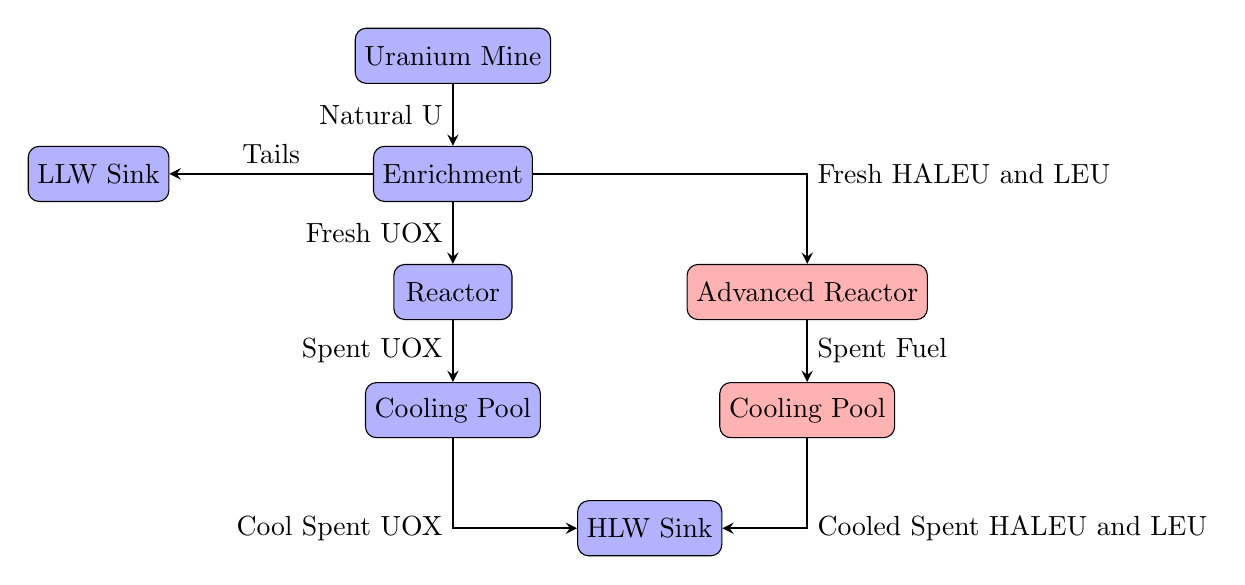
\begin{tikzpicture}[node distance=1.5cm]
        \node (mine) [facility] {Uranium Mine};
        \node (enrichment) [facility, below of=mine]{Enrichment};
        \node (reactor) [facility, below of=enrichment]{Reactor};
        \node (adv_reactor) [transition, right of=reactor, xshift=3cm]{Advanced Reactor};
        \node (wetstorage) [facility, below of=reactor]{Cooling Pool};
        %\node (drystorage) [facility, below of=wetstorage]{Dry Storage};
        \node (cooling) [transition, below of=adv_reactor]{Cooling Pool};
        \node (sinkhlw) [facility, below of=wetstorage, xshift=2.5cm]{HLW Sink};
        \node (sinkllw) [facility, left of=enrichment, xshift=-3cm]{LLW Sink};

        \draw [arrow] (mine) -- node[anchor=east]{Natural U} (enrichment);  
        \draw [arrow] (enrichment) -- node[anchor=south]{Tails}(sinkllw);
        \draw [arrow] (enrichment) -- node[anchor=east]{Fresh UOX}(reactor);
        \draw [arrow] (enrichment) -| node[anchor=west]{Fresh HALEU and LEU}(adv_reactor);
        \draw [arrow] (reactor) -- node[anchor=east]{Spent UOX}(wetstorage);
        \draw [arrow] (wetstorage) |- node[anchor=east]{Cool Spent UOX}(sinkhlw);
        %\draw [arrow] (drystorage) |- node[anchor=east]{Casked Spent UOX}(sinkhlw);
        \draw [arrow] (adv_reactor) -- node[anchor=west]{Spent Fuel}(cooling);
        \draw [arrow] (cooling) |- node[anchor=west]{Cooled Spent HALEU and LEU}(sinkhlw);`'

        \end{tikzpicture}
    \caption{Fuel cycle facilities and material flow between facilities in the 
    once-through fuel cycles modeled. Facilities in 
    blue are used in all once-through scenarios, the facilities in red are added in
    at the transition start time in the transition scenarios.}
    \label{fig:once-through_fuel_cycle}
\end{figure}

The once-through scenarios model the current fleet of \glspl{LWR} in the 
US and the transition to multiple combinations of the advanced reactors 
and different energy demand scenarios, summarized in Table 
\ref{tab:scenarios_once-through}. Scenario 1 models the \gls{LWR} fleet 
without the transition to any advanced reactor to provide a comparison with 
historic needs for a fuel cycle based on enrichments to less than 5\% $^{235}$U. 
The energy demands are based on the energy supplied by the \glspl{LWR} in 
2025 (the start of the transition). A no growth energy demand applies a 
constant demand for the energy produced by \glspl{LWR} in 2025, and a 1\% 
growth demand applies an exponential growth demand starting at the energy 
produced by \glspl{LWR} in 2025. A 1\% annual growth in demand (Scenarios 8-13) 
is less than what Dixon et al. \cite{dixon_estimated_2022} modeled
(1.2\%-2\%) but more than the average growth between 2020-2050 in the 
reference case of the 2022 \gls{EIA} Annual Energy Outlook 
\cite{us_energy_information_administration_annual_2022} (0.82\%), and 
provides a middle-ground estimate on material requirements for a growing 
energy demand. 

\begin{table}[ht]
    \centering
    \caption{Summary of the once-through fuel cycle transition scenarios.}
    \label{tab:scenarios_once-through}
    \begin{tabular}{c l l}
            \hline
            Scenario number & Reactors present & Energy growth model\\\hline
            1 & \glspl{LWR} & N/A \\
            2 & \glspl{LWR} and \gls{MMR} & No growth \\
            3 & \glspl{LWR} and Xe-100 & No growth \\
            4 & \glspl{LWR}, Xe-100, and \gls{MMR}& No growth\\
            5 & \glspl{LWR}, \gls{MMR}, and VOYGR & No growth\\
            6 & \glspl{LWR}, Xe-100, and VOYGR & No growth\\
            7 & \glspl{LWR}, Xe-100, \gls{MMR}, and VOYGR & No growth\\
            8 & \glspl{LWR} and \gls{MMR}& 1\% growth \\
            9 & \glspl{LWR} and Xe-100 & 1\% growth\\
            10 & \glspl{LWR}, Xe-100, and \gls{MMR}& 1\% growth\\
            11 & \glspl{LWR}, \gls{MMR}, and VOYGR & 1\% growth\\
            12 & \glspl{LWR}, Xe-100, and VOYGR & 1\% growth\\
            13 & \glspl{LWR}, Xe-100, \gls{MMR}, and VOYGR & 1\% growth\\
            \hline
    \end{tabular}
\end{table}

Recipes define the composition of each material in the simulation. 
Recipes for \gls{LWR} fresh and spent fuel were found in work 
by Jacobson et al. \cite{jacobson_verifiable_2010}. Section 
\ref{sec:reactor_methods} describes how this work determined recipes 
for fresh fuel in the advanced reactors. Other important recipes in the 
simulations include natural uranium (0.711\% weight fraction $^{235}$U) 
and enrichment tails (0.2\% weight fraction $^{235}$U). Spent fuel 
compositions for the Xe-100 and \gls{MMR} were obtained by performing 
depletion on Serpent \cite{leppanen_serpent_2014} models of the
cores, with Section \ref{sec:neutronics-methods} describing the models 
in more detail. The spent fuel composition for the \gls{LWR} fuel 
from Jacobson et al. were used for the VOYGR spent fuel. 

The institutions in the simulations 
govern the deployment of reactors. A \Cycamore \texttt{DeployInst} 
institution \cite{huff_fundamental_2016} deploys and decommissions the 
\glspl{LWR} according to their start and end dates. A second \Cycamore 
\texttt{DeployInst} deploys and decommissions the advanced reactors, 
based on calculations external to the \Cyclus simulations, of when 
new reactors must be deployed to meet the energy 
demand. All of the facilities and institutions in the simulation are in 
the same region, which represents that all facilities are in the same 
country. 

The advanced reactor deployment scheme preferentially deploys the advanced 
reactor with the largest power output in the scenario (e.g., Xe-100s in 
Scenario 7) until their deployment would create an oversupply of power
(i.e., the number of reactors is rounded down). 
Then the next largest reactor (e.g., VOYGRs in Scenario 7) is deployed 
until an oversupply of power would be 
created. Finally, the reactor 
with the smallest power output in the scenario (e.g., \glspl{MMR} in 
Scenario 7) is deployed until the demand is fully met (i.e., the number of 
reactors needed is rounded up). The demand 
met by deploying new reactors is the difference between the energy 
produced by previously deployed reactors and the energy demand at each 
time step. 
Figure \ref{fig:AR_deployment} illustrates how the advanced reactors 
would be deployed in Scenario 7 to meet a fictitious demand of 530 MWe. For this 
example, 5 Xe-100s, 1 VOYGR, and 1 \gls{MMR} are deployed, producing a 
total of 534 MWe. This deployment 
strategy aims to minimize the number of reactors deployed,  
minimize power oversupply, and mimic a realistic deployment strategy.

\begin{figure}[ht]
    \centering
    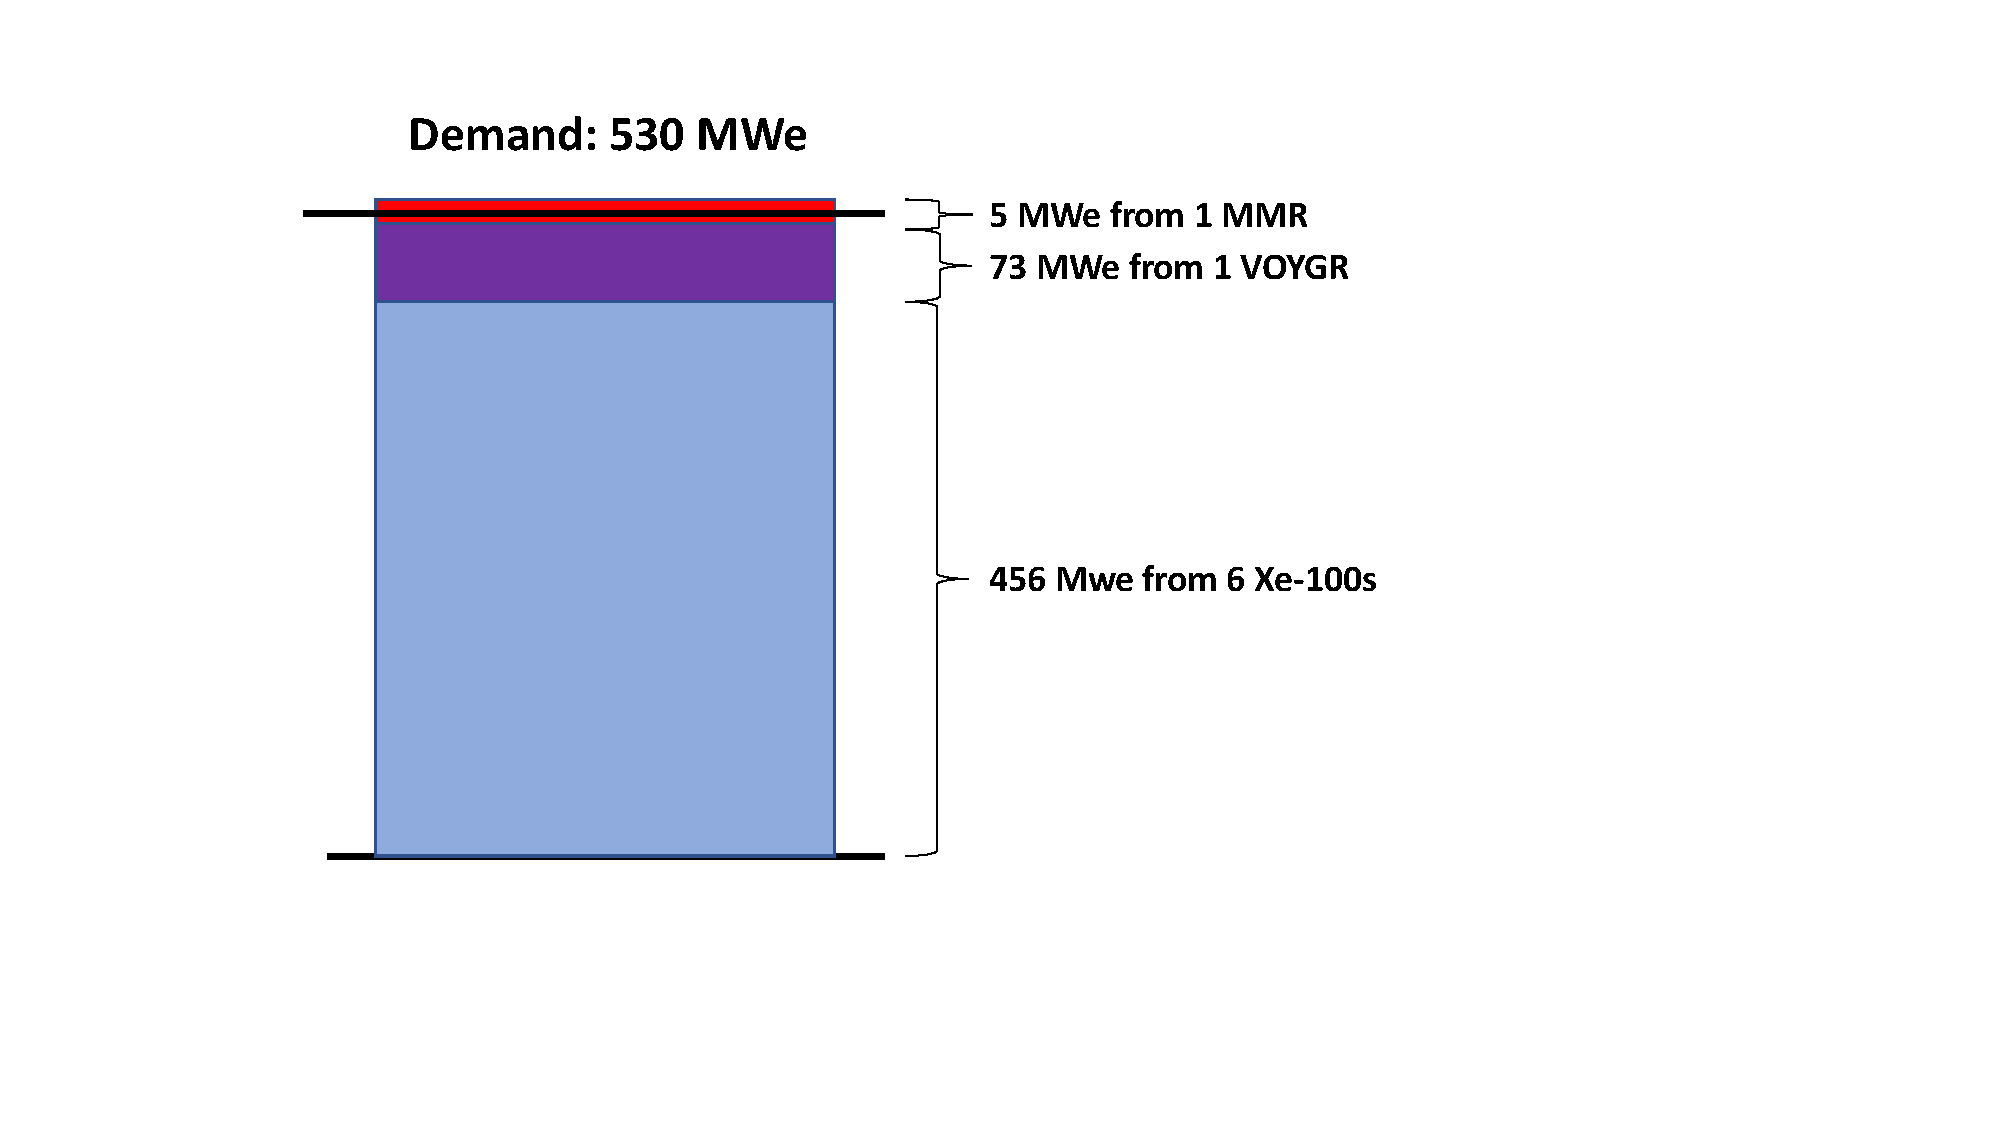
\includegraphics[scale=0.5, trim=0 100 90 0,clip]{Deployment_Scheme.pdf}
    \caption{Example of how advanced reactors are deployed in Scenario 7 
    to meet a theoretical demand of 530 MWe.}
    \label{fig:AR_deployment}
\end{figure}

This deployment strategy is used to deploy advanced reactors when there is
unmet demand in energy from the decommissioning of \glspl{LWR} or 
when the demand increases (such as in the 1\% growth scenarios). When 
there is unmet demand from the decommissioning of advanced reactors, the 
advanced reactors are redeployed on almost a one-to-one basis. A slightly
smaller number of advanced reactors may be redeployed if there is an 
oversupply of power greater than the power output of the reactor to be 
redeployed. 

\section{Recycling fuel cycle}\label{sec:recycle-methods}
Transition scenarios with a closed fuel cycle were created
to investigate how this type of \gls{NFC} affects the material requirements 
and how the recycling scheme impacts them. The scenarios investigated in 
this analysis vary by the energy demand of the scenario and the recycling 
scheme (Table \ref{tab:scenarios_recycle}). Energy demands vary 
between a no growth and a 1\% growth model, using the same 
demand curves as the once-through 
fuel cycle models. Variations in the recycling 
scheme include either a limited or a continuous recycle. Limited recycle 
scenarios assume that \gls{SNF} is recycled once and disposed of after a 
second pass through the reactor. Continuous recycling assumes that all 
\gls{SNF} is recycled an unlimited number of times until all fissile 
material has been used. Both recycling schemes were considered in the 
\acrfull{ES} \cite{wigeland_nuclear_2014}, which led to their inclusion 
in this work. Another distinction between some of the 
scenarios is if spent \gls{TRISO} fuel is recycled. \gls{TRISO} fuel is 
expensive and difficult to recycle \textbf{find citation}, and 
therefore by modeling scenarios that do and do not recycle 
\gls{TRISO} we can model realistic scenarios in which \gls{TRISO} 
is not recycled and more academic scenarios in which all spent fuel is 
recycled. 

\begin{table}[ht]
    \centering
    \caption{Summary of the recycle fuel cycle transition scenarios.}
    \label{tab:scenarios_recycle}
    \begin{tabular}{l l l l}
            \hline
            Scenario number & Energy growth model & Recycle scheme & \gls{TRISO} recycled?\\
            \hline
            14 & No growth & Limited & Yes\\
            15 & No growth & Limited & No\\
            16 & No growth & Continuous & N/A \\
            17 & 1\% growth & Limited & Yes\\
            18 & 1\% growth & Limited & No\\
            19 & 1\% growth & Continuous & N/A \\
            \hline
    \end{tabular}
\end{table}

All of the scenarios with recycling model the transition from the 
current fleet of \glspl{LWR} to the X-energy Xe-100, \gls{USNC} \gls{MMR}, 
and the NuScale VOYGR, the same as in scenarios 7 and 13. Therefore, 
the advanced reactor deployment schedules for these two scenarios are applied 
to the recycling scenarios for the appropriate energy growth model. 
This combination 
of reactors is considered for this step of the work, and not all of the 
combinations considered for the once-through scenarios, to limit the scope 
of the work while providing some comparison between the 
once-through and recycle transition scenarios. Because these scenarios 
use the same advanced reactor deployment schedule, the number of 
advanced reactors and the energy supplied are not examined in the 
results because they will be the same for each of these scenarios. Instead, 
the results of these scenarios will focus on the material requirements. 

For this work, the \glspl{LWR} and \gls{MMR} are modeled using the 
\Cycamore \texttt{Reactor} archetype. Each of these reactors use the 
fresh and spent fuel recipes that are used for the once-through scenarios. 
The Xe-100 and VOYGR are modeled using the DepleteReactor 
archetype from the OpenMCyclus library. The OpenMCyclus library was 
developed for this work, to expand the capabilities of \Cyclus archetypes 
to dynamically modeling fuel depletion during a simulation. Section 
\ref{sec:openmcyclus} provides more details on how this archetype 
works and how it compares to the \Cycamore \texttt{Reactor} 
archetype. OpenMCyclus couples with the stand-alone depletion 
solver in OpenMC \cite{romano_depletion_2021}, thus, modeling a 
reactor using this archetype requires information about the refueling 
scheme for the reactor but also one-group cross section data to perform the 
depletion. 

For the VOYGR, we generated the one-group cross section data by using the 
built-in \gls{PWR} assembly model in OpenMC. We modified this model so 
that the fuel composition matched that of the VOYGR as modeled in this 
work. For the Xe-100, we used the Serpent \cite{leppanen_serpent_2014} 
and the Xe-100-like model described in Section 
\ref{sec:xe100_serpent_model} to generate the cross section data. We 
post-processed the cross section data from Serpent to match the 
format required by OpenMC. For both reactors, we used the simplified 
depletion chain from OpenMC (referred to as the CASL chain) 
\cite{romano_depletion_2021}. Using this depletion chain results in  
adequate accuracy to the full depletion chain \cite{romano_depletion_2021}
and reduced run times compared with the full depletion chain.  

\subsection{Limited recycle scenarios}
Figure \ref{fig:limited_recycle_flow} shows the fuel cycle and material flows 
for the scenarios with limited recycling (Scenarios 14, 15, 17, and 18). 
In Scenarios 15 and 18 only the spent fuel from the 
VOYGRs is sent to the reprocessing facility, but in Scenarios 14 and 17, 
all spent fuel from the advanced reactors is sent to the 
reprocessing facility. Only the Xe-100 and VOYGRs receive \gls{MOX} fuel, 
but not the \glspl{MMR} because the \gls{MMR} does not undergo refueling, 
and therefore would not receive \gls{MOX} fuel.

\begin{figure}
    \centering
    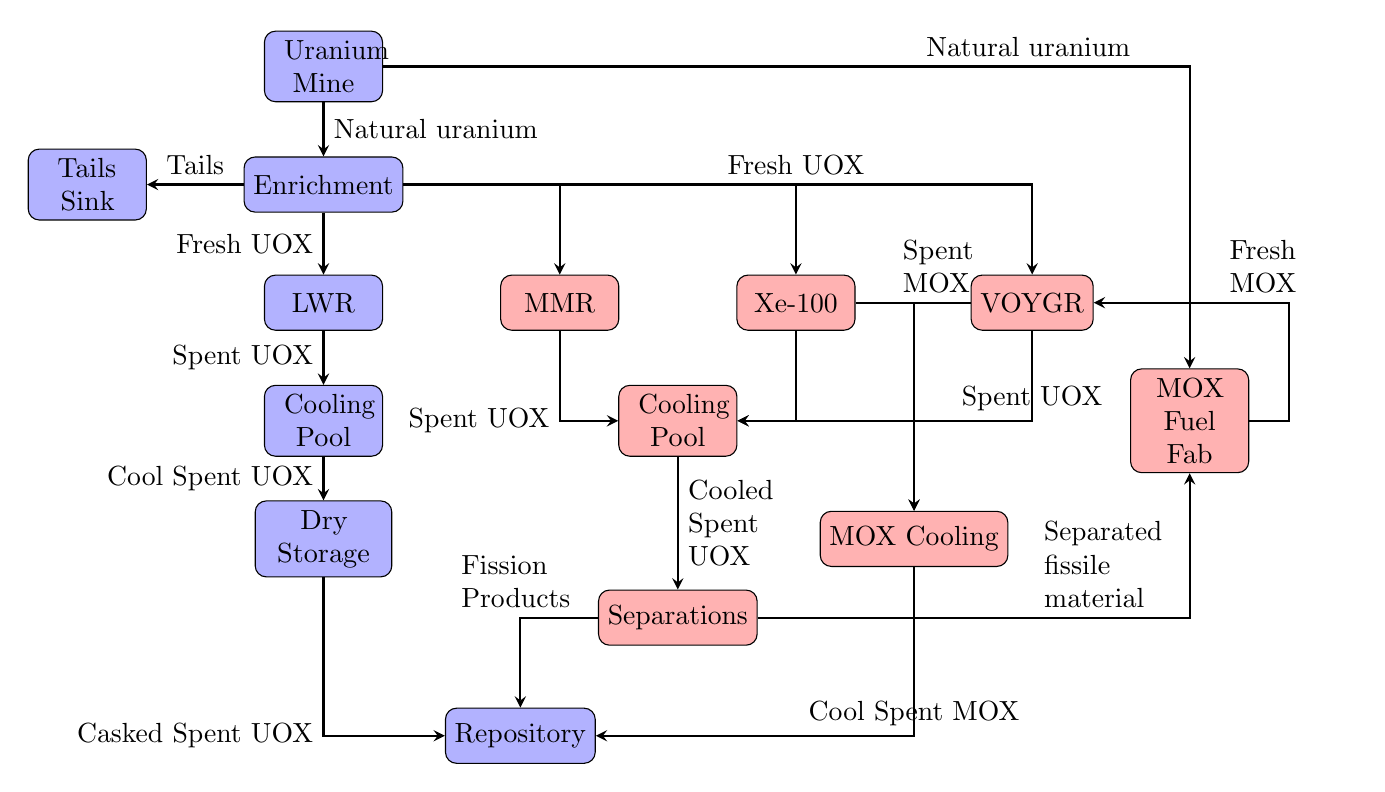
\begin{tikzpicture}[node distance=1.5cm]
        \node (mine) [facility, text width=1cm] {Uranium Mine};
        \node (enrichment) [facility, below of=mine]{Enrichment};
        \node (reactor) [facility, below of=enrichment]{LWR};
        \node (mmr) [transition, right of=reactor, xshift=1.5cm]{MMR};
        \node (xe100) [transition, right of=mmr, xshift=1.5cm]{Xe-100};
        \node (voygr) [transition, right of=xe100, xshift=1.5cm]{VOYGR};
        \node (wetstorage) [facility, below of=reactor, text width=1cm]{Cooling Pool};
        \node (drystorage) [facility, below of=wetstorage, text width=1.5cm]{Dry Storage};
        \node (cooling) [transition, below of=mmr, xshift=1.5cm, text width=1cm]{Cooling Pool};
        \node (sinkhlw) [facility, below of=drystorage, xshift=2.5cm, yshift=-1cm]{Repository};
        \node (sinkllw) [facility, left of=enrichment, xshift=-1.5cm, text width=1cm]{Tails Sink};
        \node (separation) [transition, below of=cooling, yshift=-1cm]{Separations};
        \node (mox_fab) [transition, below of=voygr,xshift=2cm, text width=1cm]{MOX Fuel Fab};
        \node (mox_cooling) [transition, below of=xe100, xshift=1.5cm, yshift=-1.5cm]{MOX Cooling};
        
        \draw [arrow] (mine) -- node[anchor=west]{Natural uranium} (enrichment);
        \draw [arrow] (enrichment) -- node[anchor=east]{Fresh UOX}(reactor);
        \draw [arrow] (enrichment) -- node[anchor=south]{Tails}(sinkllw);
        \draw [arrow] (enrichment) -| (mmr);
        \draw [arrow] (enrichment) -| node[anchor=south]{Fresh UOX}(xe100);
        \draw [arrow] (enrichment) -| (voygr);
        \draw [arrow] (reactor) -- node[anchor=east]{Spent UOX}(wetstorage);
        \draw [arrow] (wetstorage) -- node[anchor=east]{Cool Spent UOX}(drystorage);
        \draw [arrow] (drystorage) |- node[anchor=east]{Casked Spent UOX}(sinkhlw);
        \draw [arrow] (mmr) |- node[anchor=east]{Spent UOX}(cooling);
        \draw [arrow] (xe100) |- (cooling);
        \draw [arrow] (voygr) |- node[anchor=south]{Spent UOX}(cooling);
        \draw [arrow] (xe100) -| (mox_cooling);
        \draw [arrow] (voygr) -| node[anchor=south, text width=1cm, pos=0.25]{Spent MOX}(mox_cooling);
        \draw [arrow] (cooling) -- node[anchor=west, text width=1.5cm]{Cooled Spent UOX}(separation);
        \draw [arrow] (separation) -| node[anchor=south,text width=1.5cm, pos=0.4]{Separated fissile material}(mox_fab);
        \draw [arrow] (separation) -| node[anchor=south, text width=1.5cm]{Fission Products}(sinkhlw);
        \draw [arrow] (mine) -| node[anchor=south, pos=0.4]{Natural uranium} (mox_fab);
        \draw [arrow] (mox_cooling) |- node[anchor=south]{Cool Spent MOX}(sinkhlw);
        \draw [arrow] (mox_fab.east) - ++(5mm,0) |- node[anchor=south, pos=0.5, text width=1.5cm]{Fresh MOX}(voygr.east);
        %\draw [arrow] (mox_fab.east) -| ++(5mm,0) -| (xe100.north);
        \end{tikzpicture}
    \caption{Fuel cycle facilities and material flow between facilities for modeling the transition 
    to advanced reactors with a limited recycle fuel cycle. The separations facility
    is deployed in 2020, five years before the transition. Before 2020 a once-through 
    fuel cycle is used with the facilities in blue.}
    \label{fig:limited_recycle_flow}
\end{figure}

A separations facility is deployed 5 years before the transition 
begins (i.e. in 2020), as this strategy is commonly used for modeling 
transitions with recycling \cite{passerini_systematic_2014,richards_application_2021}
to ensure that enough fuel can be separated and 
processed in time for use in advanced reactors. Although this is a 
non-physical time to begin recycling in the US, using this timeline ensures 
that there will be enough reprocessed fuel to fuel all of the advanced 
reactors, and one can observe the maximum benefit of recycling. Additionally 
by using this timeline, specifically ensuring that advanced reactors 
are deployed at the same time as when they are deployed in the once-through 
transition, provides an even comparison between these fuel cycle options.
Based on the timeline of the separations facility deployment, only the 
\gls{UNF} from the \glspl{LWR} that is discharged after 2020 will 
be reprocessed. 

The separations facility separates out plutonium from the other 
materials in the fuel, emulating the aqueous reprocessing method although the 
chemistry is not explicitly modeled. The partitioning factor is 99\% for
plutonium, based on a conservative estimate of stated 
process loses for aqueous reprocessing \cite{herbst_6_2011} and the 
separation efficiency previously used in previous fuel cycle modeling 
\cite{wigeland_nuclear_2014,sunny_transition_2015}. The separated 
material from this facility is then sent to a \gls{MOX} fuel fabrication 
facility that produces \gls{MOX} with a pre-defined composition for the 
advanced reactors. To determine the plutonium fraction in the 
\gls{MOX} fuel, we calculated the plutonium equivalence of the $^{235}$U 
based on the cross section data generated from OpenMC. We assumed 
that all plutonium in the \gls{MOX} is $^{239}$Pu, even though fabricated 
\gls{MOX} will have other plutonium isotopes present, as 
a simplifying assumption. Using this 
method helps ensure that the fuel used will allow the 
reactor to run for the same cycle time and have the same assembly mass.
The separated plutonium is used as a fissile stream while the 
natural uranium from the mine are used as filler materials to 
produce \gls{MOX}. The separation step is modeled using the \Cycamore 
\texttt{Separations} archetype, and the \gls{MOX} fuel fabrication is modeled 
using the \Cycamore \texttt{Mixer} archetype. The \texttt{Mixer} archetype 
combines the separated plutonium and natural uranium material 
streams in the constant ratios required to produce the \gls{MOX} fuel
that corresponds to composition for each reactor. 

\subsection{Continuous recycle scenarios}
Figure \ref{fig:continuous_recycle_flow} shows the facilities and material 
flow for the continuous recycle fuel cycle (Scenarios 16 and 19). Continuous recycle 
requires a fast reactor, but all of the reactors considered in this 
work so far have a thermal neutron energy spectrum. Therefore, the advanced 
reactors used in the other scenarios are replaced with a \gls{SFR}. 
The fast reactor is modeled based on the PRISM design from 
\gls{GEH} in the \gls{UNF} Recycle mode \cite{triplett_prism:_2012}, based on 
the availability of open-source information to accurately model the design
and fuel compositions. We defined the \gls{SFR} 
to prefer reprocessed fuel over \gls{HALEU} fuel. The reprocessed fuel 
composition is based on published information about the metallic fuel 
composition \cite{triplett_prism:_2012,sumner_effects_2011}. 
The \gls{HALEU} was determined 
based on the one-group cross section data of the OpenMC model described 
below and calculating the plutonium equivalence of uranium for the core.

\begin{figure}
    \centering
    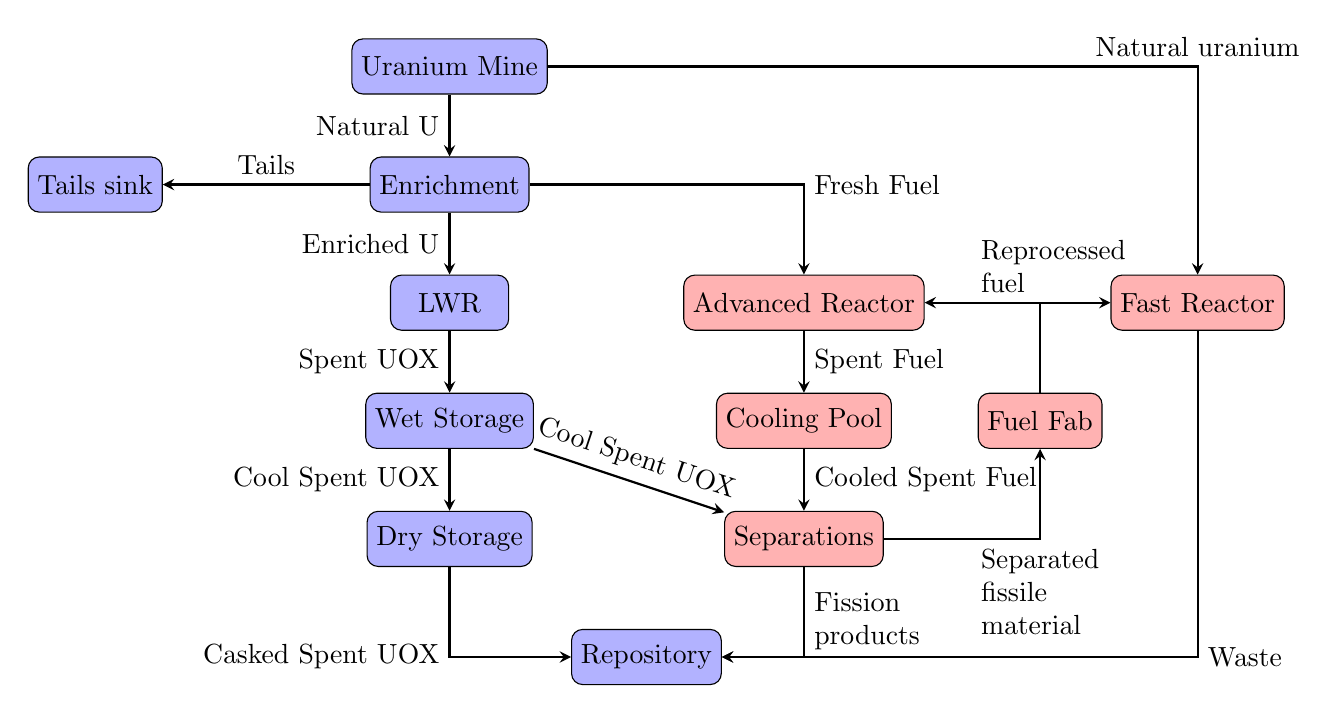
\begin{tikzpicture}[node distance=1.5cm]
        \node (mine) [facility] {Uranium Mine};
        \node (enrichment) [facility, below of=mine]{Enrichment};
        \node (reactor) [facility, below of=enrichment]{LWR};
        \node (adv_reactor) [transition, right of=reactor, xshift=3cm]{Advanced Reactor};
        \node (wetstorage) [facility, below of=reactor]{Wet Storage};
        \node (drystorage) [facility, below of=wetstorage]{Dry Storage};
        \node (cooling) [transition, below of=adv_reactor]{Cooling Pool};
        \node (sinkhlw) [facility, below of=drystorage, xshift=2.5cm]{Repository};
        \node (sinkllw) [facility, left of=enrichment, xshift=-3cm]{Tails sink};
        \node (separation) [transition, below of=cooling]{Separations};
        \node (fuelfab) [transition, below of=adv_reactor,xshift=3cm]{Fuel Fab};
        \node (sfr) [transition, right of=adv_reactor, xshift=3.5cm]{Fast Reactor};

        \draw [arrow] (mine) -- node[anchor=east]{Natural U} (enrichment);
        \draw [arrow] (enrichment) -- node[anchor=east]{Enriched U}(reactor);
        \draw [arrow] (enrichment) -- node[anchor=south]{Tails}(sinkllw);
        \draw [arrow] (enrichment) -| node[anchor=west]{Fresh Fuel}(adv_reactor);
        \draw [arrow] (reactor) -- node[anchor=east]{Spent UOX}(wetstorage);
        \draw [arrow] (wetstorage) -- node[anchor=east]{Cool Spent UOX}(drystorage);
        \draw [arrow] (drystorage) |- node[anchor=east]{Casked Spent UOX}(sinkhlw);
        \draw [arrow] (adv_reactor) -- node[anchor=west]{Spent Fuel}(cooling);
        \draw [arrow] (cooling) -- node[anchor=west]{Cooled Spent Fuel}(separation);
        \draw [arrow] (separation) -| node[anchor=north, text width=1.5cm]{Separated fissile material}(fuelfab);
        \draw [arrow] (fuelfab) |- node[anchor=south, text width=1.5cm]{Reprocessed fuel}(sfr);
        \draw [arrow] (fuelfab) |- (adv_reactor);
        \draw [arrow] (separation) |- node[pos= 0.3, anchor=west, text width = 1.5cm]{Fission products}(sinkhlw);
        \draw [arrow] (wetstorage) -- node[sloped, anchor=south]{Cool Spent UOX}(separation);
        \draw [arrow] (sfr) |- node[anchor=west]{Waste}(sinkhlw);
        \draw [arrow] (mine) -| node[anchor=south]{Natural uranium}(sfr);

        \end{tikzpicture}
    \caption{Fuel cycle facilities and material flow between facilities for modeling the transition 
    to advanced reactors with a continuous recycle fuel cycle. Before 2020 a once-through 
    fuel cycle is used with the facilities in blue. Facilities in red are deployed 
    in 2025, and represent all of the facilities and material flows in red in 
    Figure \ref{fig:limited_recycle_flow}.}
    \label{fig:continuous_recycle_flow}
\end{figure}

\begin{table}
    \centering
    \begin{threeparttable}

    \caption{Fast reactor design specification.}
    \label{tab:fast_rx}
    \begin{tabular}{l l}
        \hline
        Design Criteria & PRISM \cite{triplett_prism:_2012,fichtlscherer_assessing_2019}\\
        \hline
        Reactor type & Sodium Fast Reactor\\
        Power Output (MWth) & 840 \\
        Capacity Factor & 90\%\tnote{1} \\
        Enrichment (wt\% fissile Pu) &  11.3/13.5\tnote{2}\\
        Cycle Length (yrs) & 1 \\
        Number of cycles &  4\\
        Fuel form &  Metallic \\
        Discharge fuel burnup (GWd/MTU) & 87.51 \\
        Reactor Lifetime (yrs)&  60\\
        \hline
    \end{tabular}
    \begin{tablenotes}
        \item [1] Assumed value
        \item [2] The PRISM in UNF Recycle mode has two different drive fuel compositions,
                  which are averaged based on the number of each assembly type to determine 
                  the fresh fuel composition for this reactor.
    \end{tablenotes}
\end{threeparttable}
\end{table}

We developed an OpenMC model of the PRISM reactor (shown in 
Figure \ref{fig:prism_model}) and used OpenMC to generate the one-group 
cross section data needed for depletion. Information about the 
dimensions and core configuration of the reactor were found in 
\cite{triplett_prism:_2012,fichtlscherer_assessing_2019}. 
These sources also provided some 
information about the fresh fuel composition, which we supplemented 
with the isotopic ratios defined for the S-PRISM reactor (a 1000 MWth
\gls{SFR} of a similar design) in \cite{sumner_effects_2011}.
We then used the transport-coupled depletion solver in OpenMC to 
obtain compositions for each fuel batch at the beginning of cycle 
in this reactor. After revising the model to include each of the 
batch beginning of cycle compositions in the placements given 
in \cite{fichtlscherer_assessing_2019}, we ran the model 
through OpenMC again to obtain the one-group cross section data 
required for modeling this reactor design in OpenMCyclus. We calculated
the \gls{HALEU} composition required for this fuel cycle based on the 
plutonium equivalence of uranium in this system.

\begin{figure}[h!]
    \centering
    \begin{subfigure}[b]{0.48\textwidth}
        \centering
        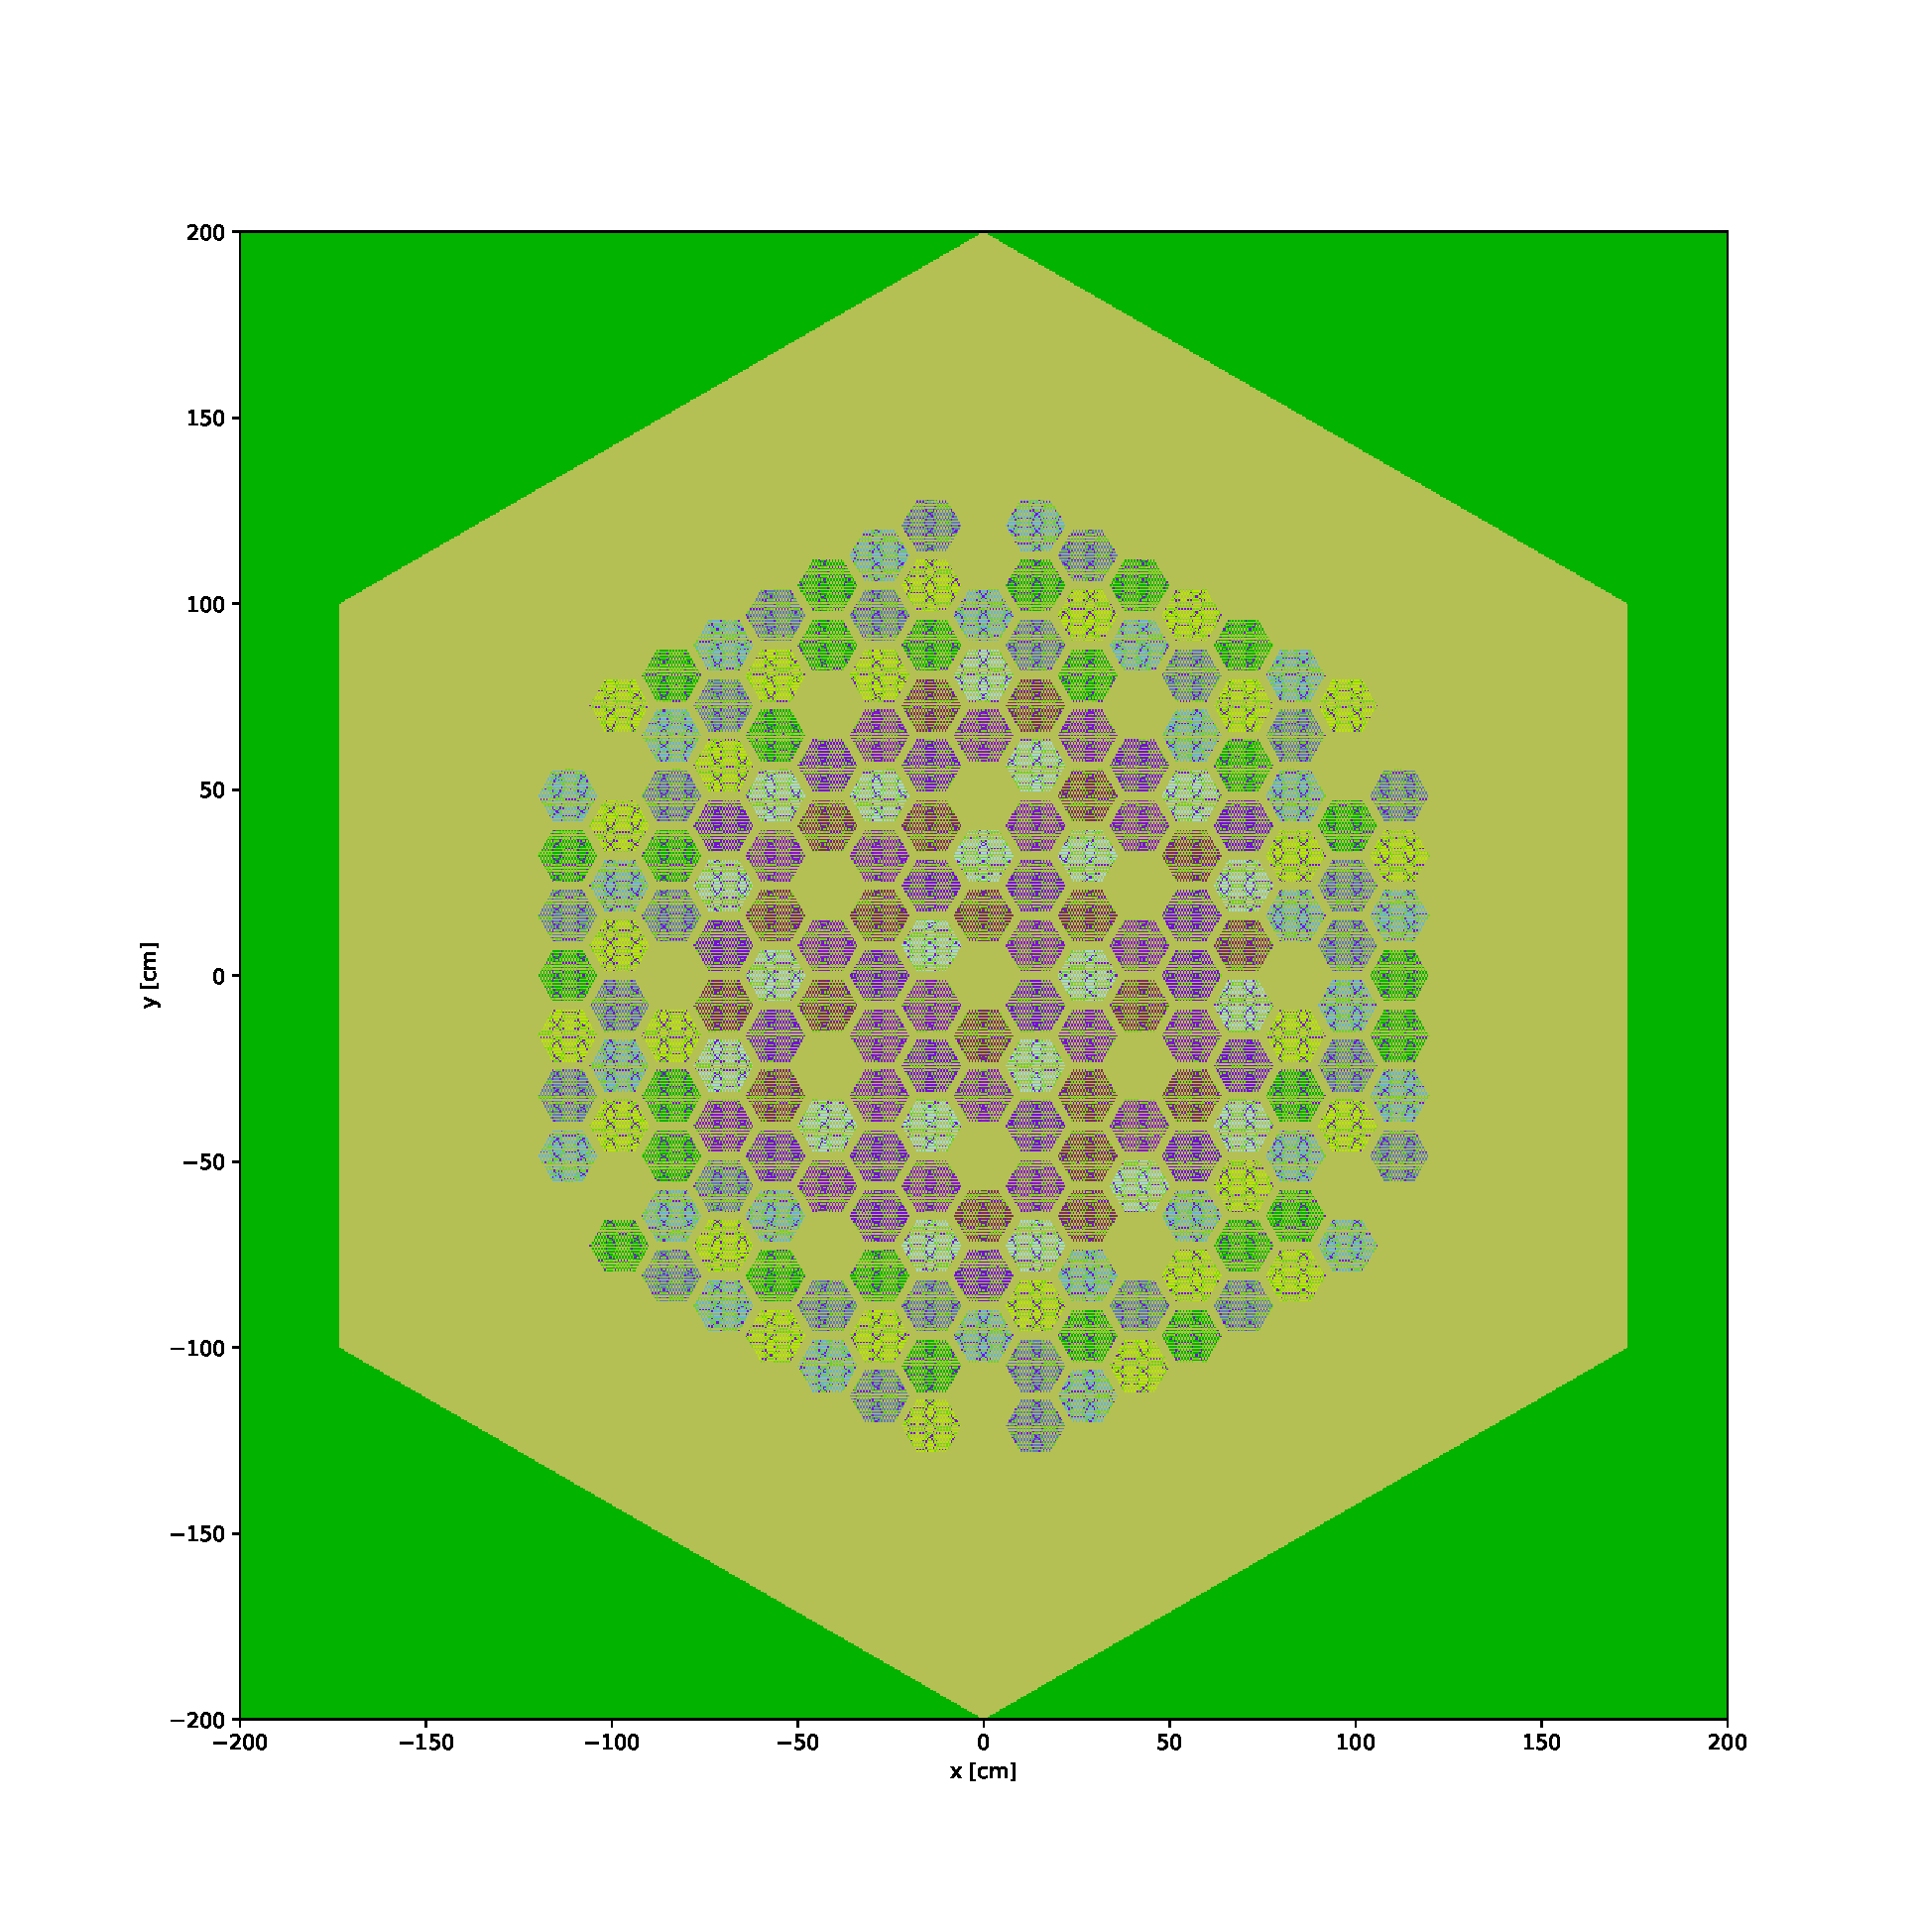
\includegraphics[width=\textwidth]{sfr_eq_core.pdf}
        \caption{Radial view of the entire PRISM model.}
        \label{fig:prism_lattice}
    \end{subfigure}
    \hfill
    \begin{subfigure}[b]{0.48\textwidth}
        \centering
        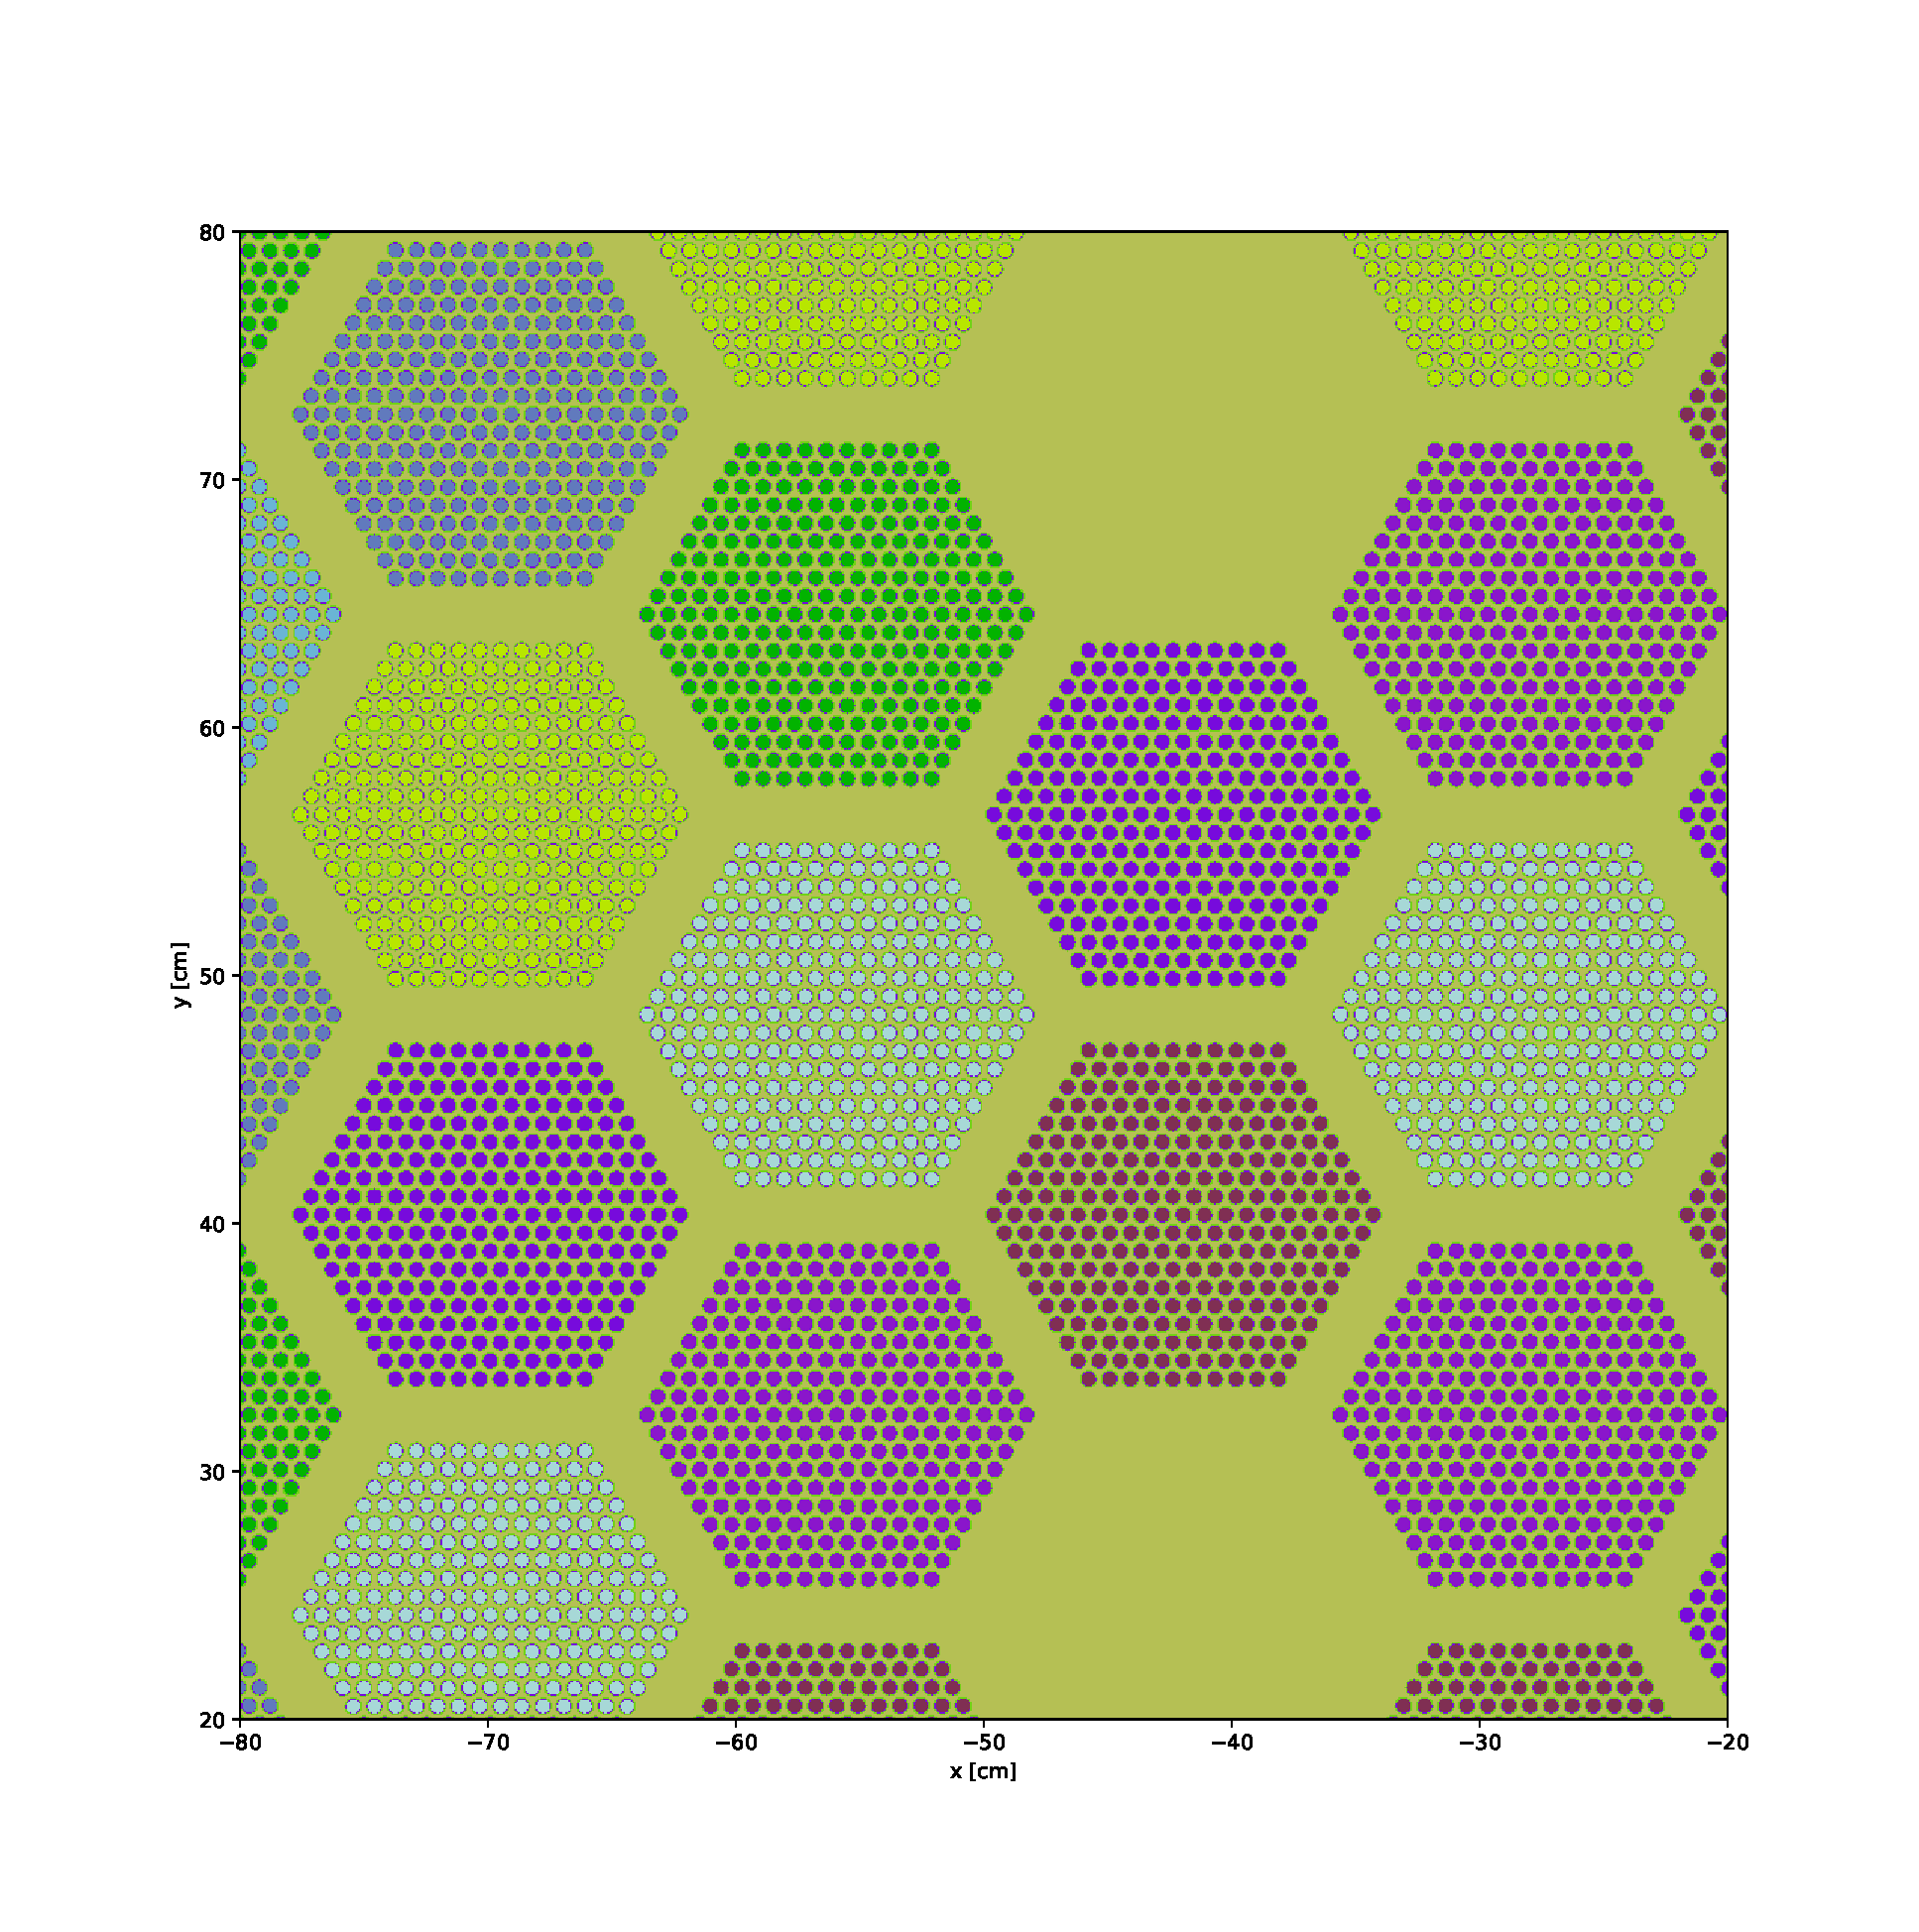
\includegraphics[width=\textwidth]{sfr_eq_core_zoom.pdf}
        \caption{Detailed view of the assembly lattice for each 
        fuel type.}
        \label{fig:prism_lattice_zoom}
    \end{subfigure}
    \hfill            
    \caption{Full and zoomed in OpenMC models of the PRISM reactor, based 
    on information in \textbf{citations}. The gold material is the 
    sodium coolant, the purple is the inner fuel assemblies, and the 
    light green is the outer fuel assemblies. }
    \label{fig:prism_model}
\end{figure}

To support using reprocessed fuel in the fast reactor, 
the separations facility is deployed in 2020, similar to in the 
limited recycling scenarios, and uranium and transuranic elements 
(neptunium, plutonium, americium, and curium) are separated out from 
the spent fuel with 99\% efficiency. If not enough reprocessed fuel is 
available to support the fast reactor fleet, then \gls{HALEU} is used 
to fuel the reactors, but the reactors have a preference for reprocessed 
fuel over \gls{HALEU}. We calculated the fuel mass using Eq. \ref{eq:fuel_mass},
and divided as needed for the mass of each assembly in the core. 
We also calculated the deployment scheme for this reactor using the 
same methodology described in Section \ref{sec:reactor_methods}, based on 
the applicable demand curve (no growth for Scenario 16 and 1\% growth 
for Scenario 19), the power output of the \gls{SFR}, and the capacity 
factor of the \gls{SFR}.

\section{OpenMCyclus}\label{sec:openmcyclus}
OpenMCyclus is an archetype library that holds the DepleteReactor 
archetype. Currently, OpenMCyclus only holds this one archetype, so 
the two terms are used synonymously here. OpenMCyclus couples 
\Cyclus with the stand-alone depletion solver in OpenMC 
\cite{romano_depletion_2021} to provide 
dynamic updates of spent fuel composition during a fuel cycle simulation.
We decided to coupled with the depletion solver in OpenMC because 
of the open-source nature of OpenMC and its rich Python \gls{API}. 
The open-source nature of OpenMC complements the open-source nature 
of \Cyclus to prevent creating additional obstacles in using the archetype. 
Additionally, the Python \gls{API} of OpenMC complements the Python 
\gls{API} of \Cyclus, aiding in the development of the archetype. 
There are two primary components to OpenMCyclus: fuel depletion and 
transmutation and the material handling. 

\subsection{Fuel depletion and transmutation} \label{sec:transmute}
The depletion of fuel in this archetype is performed through a coupling with 
the depletion solver in OpenMC. The depletion solver in OpenMC solves a system 
of first-order ODEs that describes 
the rate of change of each nuclide as a function of production and loss 
mechanisms \cite{romano_depletion_2021}. OpenMC applies a \gls{CRAM} solver 
and multiple time integration methods to solve the system of equations, which 
has been shown to have good agreement with the depletion solver in Serpent 
\cite{romano_depletion_2021}. OpenMC provides this capability in two primary 
forms: transport dependent and transport independent solvers. To simplify 
the information needed and reduce run times, OpenMCyclus uses the transport 
independent solver through the \texttt{IndependentOperator} class of the 
\texttt{openmc.deplete} module. 

Use of this class requires users to provide information including 
one-group microscopic cross section data, depletion chain data, the 
number of depletion steps, 
power level, and material compositions for the fuel. The multi-group 
cross section data must be provided by the user through a ``.csv'' file by 
specifying a path to the file, assumed to be titled ``micro\_xs.csv'' by the 
archetype. This data can be obtained by running a transport calculation 
of the desired reactor geometry using OpenMC or another transport solver. 
The depletion chain data is an ``.xml'' file that is assumed to be in the 
same directory as the cross section data, under a filename that is specified 
by the user.
The depletion steps are 30 days each (corresponding to 1 month), 
with one depletion step for each month of the operating cycle, as defined by 
the user. The power level is defined by the user, and is converted from 
MW to W (units assumed by \Cyclus to units assumed by OpenMC). Each of these 
variables (depletion chain data file name, path to the cross section data and 
depletion chain data, the number of depletion steps, and the power level) are 
defined by the user through the \Cyclus input file then passed from the archetype 
to OpenMC. The material compositions are located in an ``.xml'' file 
(assumed to be in the same directory as the cross section and depletion 
chain data, and assumed to be titled ``materials.xml''). The information 
in this file is updated by the archetype to 
contain the composition of each assembly in the reactor when depletion is 
performed. The updated information in is then read in
by OpenMC to define the materials for depletion. 

To account for multiple batches of fuel in the core, all of the assemblies 
are depleted and have their compositions updated 
at the end of each cycle, with the depletion time equaling one cycle 
length. This methodology differs from the \Cycamore 
\texttt{Reactor} archetype, which transmutes the composition of only the 
number of 
assemblies in a batch, and immediately changes the composition from that 
of the fresh fuel to that of spent fuel at the end of each cycle before the 
assemblies are discharged. Therefore, by accounting for 
changes in fresh fuel composition (e.g., UOX to MOX) and multiple 
batches in a core, OpenMCyclus is expected to be more sensitive to 
changes in spent fuel composition than the \Cycamore Reactor archetype. 
Additionally, the \Cycamore Reactor assumes that all spent fuel has the 
same composition, so even assemblies that are discharged after only one 
cycle have the same composition as those that are discharged after the
Additionally, when a reactor facility is decommissioned, the default behavior 
of the \Cycamore \texttt{Reactor} archetype is to transmute only half of the assemblies 
in the core, while the OpenMCyclus archetype transmutes all of the assemblies. 
This setting in the \Cycamore \texttt{Reactor} (\texttt{decom\_transmute\_all}) can be 
toggled to \texttt{True} so that both archetypes have the same behavior.

OpenMC has two stand-alone depletion solvers that differ on if cross section 
data is updated during depletion. OpenMCyclus uses the solver that does 
not update the cross section data. Using this method increases 
the differences in the spent fuel composition compared with when the depletion 
is performed with transport \textbf{see if Olek has published his paper yet},
but this expense is taken in favor of improved computational performance.

\subsection{Material handling}
The material handling of the OpenMCyclus DepleteReactor archetype 
includes how material is transferred within different inventories 
in the archetype, how the archetype interacts with the \gls{DRE}, 
and how these interactions are recorded to the database. 

The DepleteReactor has three different material inventories that 
are internal to the archetype: ``fresh fuel'', ``core'', and ``spent 
fuel''. Each of these inventories are 
\texttt{cyclus.typesystem.ResBufMaterialInv} objects, which means that 
the material objects (i.e., fuel) can be moved between the different 
inventories as needed, and each inventory has a defined capacity. Movements 
between these inventories are not recorded to the database. The fresh 
fuel inventory represents extra fuel that is kept on site at the 
facility. The core inventory represents the fuel in the core 
and used for operating the reactor. The spent fuel inventory 
represents fuel that is finished in the core, and has been fully 
transmuted to the spent fuel composition. Material requests that 
are traded into the archetype can be placed in the fresh fuel 
or core inventories, based on the capacities of each. The 
material in the spent fuel inventory is used to generate bids 
for requests, and is traded away to other facilities when the bids 
are matched with a request by the \gls{DRE}. 

The frequency of material movement between these inventories and 
the timing of requests and bids in the \gls{DRE} are based on 
the user-defined cycle length and refuel time state variables. 
A reactor agent (a deployed prototype) requests enough fuel assemblies 
to fill the fresh fuel and core inventories.
Each fuel assembly to fill the fresh fuel and core inventories 
is a separate request, with each request 
being exclusive (i.e., partial fulfillment of the request by another 
agent is not allowed). If multiple commodities can meet a request for 
an assembly (e.g., UOX or MOX assemblies), then all of the possible 
commodities are requested through mutual requests based on user-defined 
preferences for each commodity. Materials are requested in quantities 
to match the user-defined assembly mass size. Information about the 
materials is recorded to the output database, including the 
commodity name, material mass, sending prototype, and the receiving 
prototype. If the agent 
receives enough fuel and the core inventory is filled, then the 
agent begins its operating cycle. During the operating cycle, the 
reactor is recorded as producing the user-defined power each time step 
of the cycle, and will only request more fuel assemblies if the 
fresh fuel inventory is not filled. At the end of the operating 
cycle, the fuel in the core is transmuted as described in Section 
\ref{sec:transmute}, and one batch of fuel (a user-defined state variable)
is discharged from the core inventory to the spent fuel inventory. 
If there is any fuel in the fresh fuel inventory, then it is 
loaded into the core. Then more fuel for the fresh fuel and the 
core inventories are requested from other facilities, and the 
materials in the spent fuel inventory are traded away if requested 
by other facilities. Before starting the next operating cycle, the 
facility experiences a refueling period, that lasts as long as the 
user-defined state variable. During this period, the facility does 
not produce any power. If the core is not full or within the operating 
cycle, then it does not produce any power. After the refueling period 
ends, the facility 
enters back into the operating cycle and repeats the process until it 
is retired and decommissioned. 

When the facility reaches the end of its lifetime, all of the fuel in 
the core is transmuted one final time and all of the 
assemblies are discharged from the core to the spent fuel
inventory. If any assemblies in the fresh fuel inventory, then 
they are also moved to the spent fuel inventory to be traded 
away to other facilities. Once the core and spent fuel are 
both empty, the facility is decommissioned and exits the simulation.

\subsection{Comparison with \Cycamore Reactor}
To verify the results from OpenMCyclus, we created a sample fuel cycle 
scenario to model with the \Cycamore Reactor archetype and the 
OpenMCyclus DepleteReactor archetype. All of the code used to define the 
scenarios, generate data, and the analysis are publicly available 
\textbf{create zenodo object for Comparison files}. The fuel cycle is 
shown in Figure 
\ref{fig:comparison}. Each of the non-reactor facilities are defined 
using archetypes in the \Cycamore library, with the \Cycamore \texttt{Mixer}
defining the ``MOX Fuel Fab'' agent. The \texttt{Mixer} agent takes in multiple 
material streams and combines them in a user-defined ratio to produce 
a final output stream. For this scenario, the separated fissile plutonium 
and natural uranium are arbitrarily combined in a 1:9 ratio (10\% 
plutonium and 90\% natural uranium). 

\begin{figure}
    \centering
    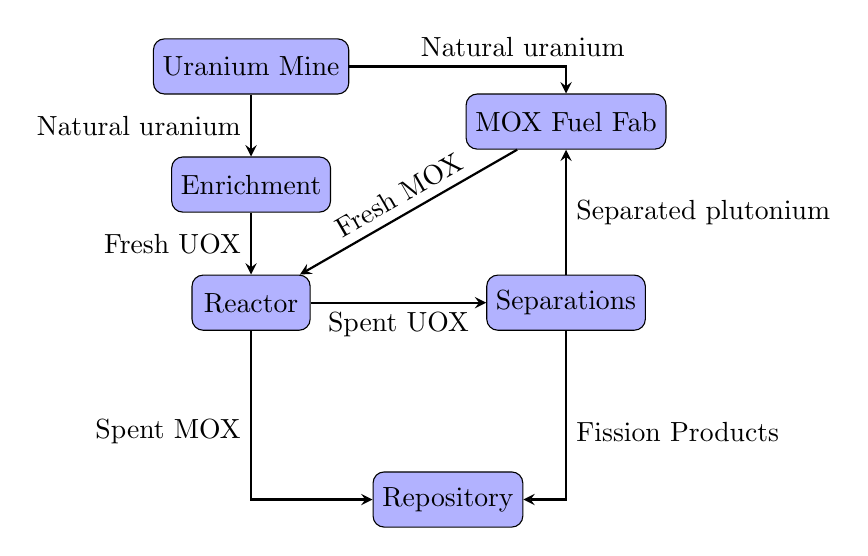
\begin{tikzpicture}[node distance=1.5cm]
        \node (mine) [facility] {Uranium Mine};
        \node (enrichment) [facility, below of=mine]{Enrichment};
        \node (reactor) [facility, below of=enrichment]{Reactor};
        \node (sinkhlw) [facility, below of=reactor, xshift=2.5cm, yshift=-1cm]{Repository};
        \node (separation) [facility, right of=reactor, xshift=2.5cm]{Separations};
        \node (mox_fab) [facility, above of=separation, yshift=0.8cm]{MOX Fuel Fab};
        
        \draw [arrow] (mine) -- node[anchor=east]{Natural uranium} (enrichment);
        \draw [arrow] (enrichment) -- node[anchor=east]{Fresh UOX}(reactor);
        \draw [arrow] (reactor) -- node[anchor=north]{Spent UOX}(separation);
        %\draw [arrow] (cooling) -- node[anchor=west, text width=1.5cm]{Cooled Spent UOX}(separation);
        \draw [arrow] (separation) -- node[anchor=west]{Separated plutonium}(mox_fab);
        \draw [arrow] (separation) |- node[anchor=west, pos=0.3]{Fission Products}(sinkhlw);
        \draw [arrow] (mine) -| node[anchor=south, pos=0.4]{Natural uranium} (mox_fab);
        \draw [arrow] (reactor) |- node[anchor=east, pos=0.3]{Spent MOX} (sinkhlw);
        \draw [arrow] (mox_fab) -- node[anchor=south, sloped]{Fresh MOX} (reactor);
        %\draw [arrow] (mox_fab.east) -| ++(5mm,0) -| (xe100.north);
        \end{tikzpicture}
    \caption{Fuel cycle facilities and material flow between facilities for the 
    sample fuel cycle scenarios used to compare the results of the \Cycamore Reactor 
    and OpenMCyclus DepleteReactor archetypes. }
    \label{fig:comparison}
\end{figure}

The entire simulation is 200 months. Reactors are deployed using the 
\Cycamore \texttt{DeployInst} institution archetype: 2 at time step 1, 
1 at time step 
50, 1 at time step 100, and 1 at time step 150. The reactors have a lifetime 
of 60 time steps, cycle length of 12 time steps, refueling length of 1 
time step, three batches per core, one assembly per batch, a power output of 
195 W, and an assembly size of 0.00602 kg. The reactors prefer MOX over UOX. 
 
To obtain a spent fuel composition for the \Cycamore \texttt{Reactor} 
archetype and cross section data for the DepleteReactor archetype, we 
used the pin cell example model in OpenMC \textbf{citation}. 
Using this 
small model is a simplifying assumption about the size of the reactors, 
and led to the small power level and assembly mass of the prototypes. 
We used this model in OpenMC to generate the one-group cross 
section data required to define the \texttt{IndependentOperator} class 
in OpenMC. Using this cross section data, we depleted the pin cell 
model using OpenMC to obtain the spent UOX and 
spent MOX compositions, with the depletion modeling the entire time that 
an assembly would be in the the core (i.e., 36 months straight). 
These compositions were then converted into recipes for use in 
\Cyclus.
The one-group cross section data from OpenMC was then used to run 
OpenMCyclus, ensuring that the same data is used for both archetypes.  

\begin{table}
    \centering 
    \caption{Compositions for fresh fuel used in the comparison between 
    the \Cycamore \texttt{Reactor} and the OpenMCyclus DepleteReactor 
    archetypes.}
    \label{tab:comparison_comps}
    \begin{tabular}{c c c c c c}
        \hline
        Recipe name & $^{235}$U ao & $^{238}$U & $^{16}$O ao & $^{239}$Pu ao & $^{240}$Pu ao\\
        \hline
        Fresh UOX & 0.010  & 0.323  & 0.667 & 0     & 0 \\
        Fresh MOX & 0.0097 & 0.3137 & 0.667 & 0.009 & 0.0006\\
        \hline
    \end{tabular}
\end{table}

We ran the scenario with the \Cycamore \texttt{Reactor} archetype twice, 
toggling the \texttt{decom\_transmute\_all} setting between \texttt{True}
and \texttt{False}. Toggling this setting allows us to explore how the 
different possible methodologies to handle the fuel upon a facility 
decommissioning in the \Cycamore \texttt{Reactor} affects the results of 
the simulation, and provide a more comprehensive comparison between the 
two archetypes. We compared the archetypes based on the energy generated 
by the reactor prototypes and the transactions of fresh fuel, spent fuel, 
and separated plutonium. 

Figure \ref{fig:comparison_power} shows the power provided from the
reactor prototypes in the scenario when each of the archetypes were used.
It is important to compare this property of the archetypes because many 
fuel cycle scenarios are designed based on deploying reactors to meet a 
specific power demand. 
There is perfect agreement between the archetypes, even with the different 
settings for the \Cycamore \texttt{Reactor}. At the start of the scenario, 
the prototypes produce 390 W of power, because two reactors are 
deployed. When the third reactor is deployed at time step 50, 
the power provided increases to 585 W. When there is only one  
reactor deployed (e.g., between time steps 63-99) 195 W of power 
are produced. Every 13th time step after a reactor facility deploys, 
the facility produced 0 W of power, signifying that it is refueling.

\begin{figure}[ht]
    \centering 
    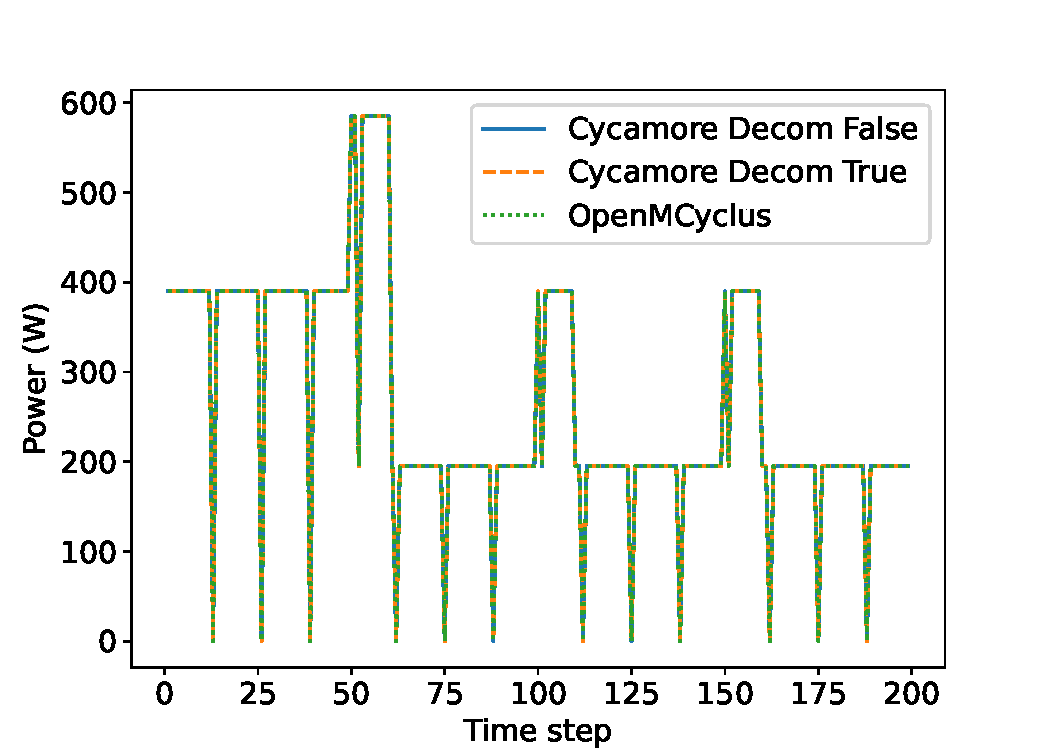
\includegraphics{comparison_energy.pdf}
    \caption{Comparison of power provided from reactor prototypes 
    when comparing the \Cycamore \texttt{Reactor} and OpenMCyclus 
    DepleteReactor archetypes.}
    \label{fig:comparison_power}
\end{figure}

Figure \ref{fig:comparison_fuel} shows the transactions of UOX and 
MOX fuel to the facilities when each archetype is used. There are 
differences between the archetypes in when they receive each fuel type. 
However, the total amount of fuel and when the fuel is received is in 
perfect agreement between all three scenarios. At each time step that 
a reactor facility is commissioned, a full core's worth of fuel (i.e., 
three assemblies) are sent to the reactor. The reactors also receive fuel 
at the correct intervals for refueling (every thirteen months or twelve 
after deployment because of the lack of refueling period). The differences 
that arise between the archetypes is in how much of each fuel commodity 
is received at each time step. Because the \gls{MOX} fuel is preferred 
over the \gls{UOX} fuel, the supply of plutonium available to create the 
\gls{MOX} fuel is the driving factor of this difference and the primary 
difference between these scenarios. 

\begin{figure}
    \centering
    \begin{subfigure}[b]{0.48\textwidth}
        \centering
        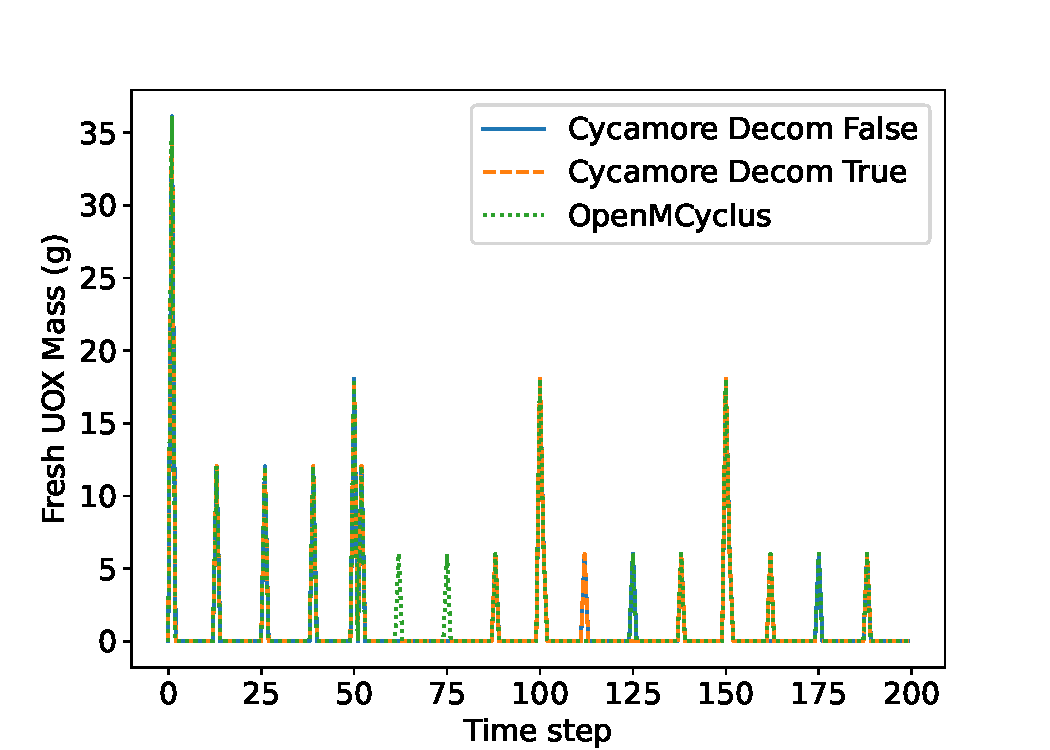
\includegraphics[trim=0 0 30 20,clip,width=\textwidth]{comparison_uox.pdf}
        \caption{Fresh UOX.}
        \label{fig:comparison_uox}
    \end{subfigure}
    \hfill
    \begin{subfigure}[b]{0.48\textwidth}
        \centering
        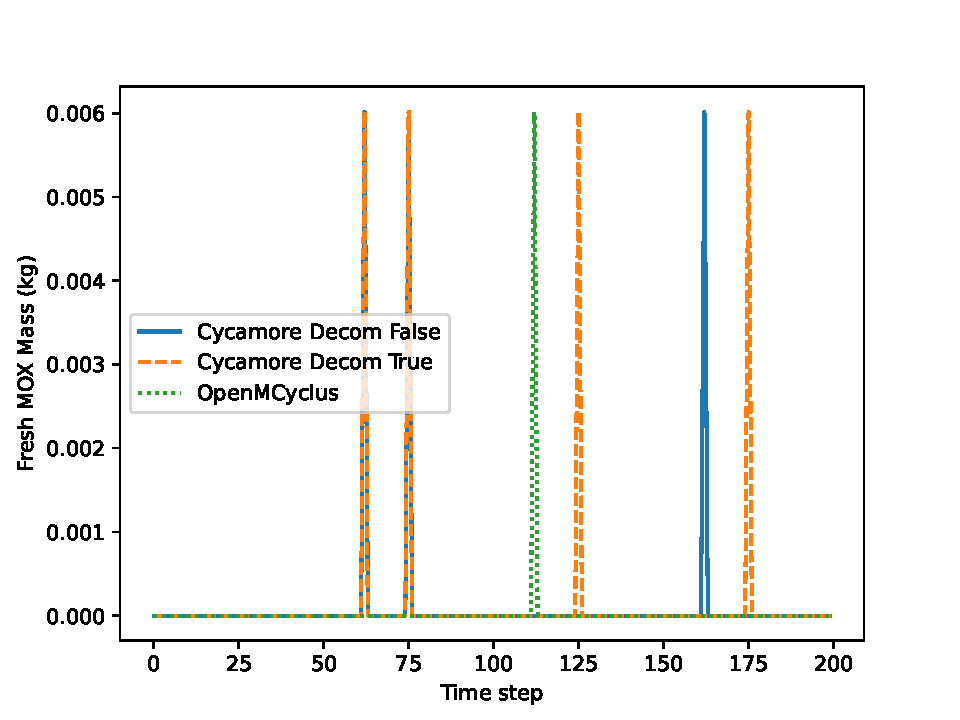
\includegraphics[trim=0 0 30 20,clip,width=\textwidth]{comparison_mox.pdf}
        \caption{Fresh MOX.}
        \label{fig:comparison_mox}
    \end{subfigure}
       \caption{Transactions of the fresh fuel commodities to the 
       reactor facilities when defined with each archetype and 
       setting.}
       \label{fig:comparison_fuel}
\end{figure}

Figure \ref{fig:comparison_spentfuel} shows the transactions of 
spent fuel from the reactors to the separations facility in each 
scenario. There is more variation between the scenarios with the 
\Cycamore \texttt{Reactor} archetype and the scenario with OpenMCyclus. 
The differences in fresh fuel commodities received by the 
reactor facilities propagate to differences in the spent fuel commodity 
discharged by the reactors in each scenario. The timing and quantity of 
fuel traded for non-retirement transactions is consistent between all 
three scenarios. However, there are differences in the spent fuel 
transactions that correspond to fuel discharged at the retirement of the 
facilities. The OpenMCyclus archetype discharges all of the assemblies 
in the same time step that the reactor retires. However, the \Cycamore 
\texttt{Reactor} archetype discharges 2/3 of the assemblies in the same 
time step that the facility retires, and the remaining 1/3 of the assemblies 
in the next time step. The behavior of the \Cycamore \texttt{Reactor} 
upon retirement is consistent regardless of the \texttt{decom\_transmute\_all}
setting. This difference in transactions identifies a methodology 
difference between the two archetypes. However, it only affects a 
scenario when a reactor facility is retired, and a one time step difference 
in when the fuel from the core is traded away is not large. Therefore, 
this methodology difference is not expected to lead to large differences 
in the behavior of a scenario. 

\begin{figure}
    \centering
    \begin{subfigure}[b]{0.48\textwidth}
        \centering
        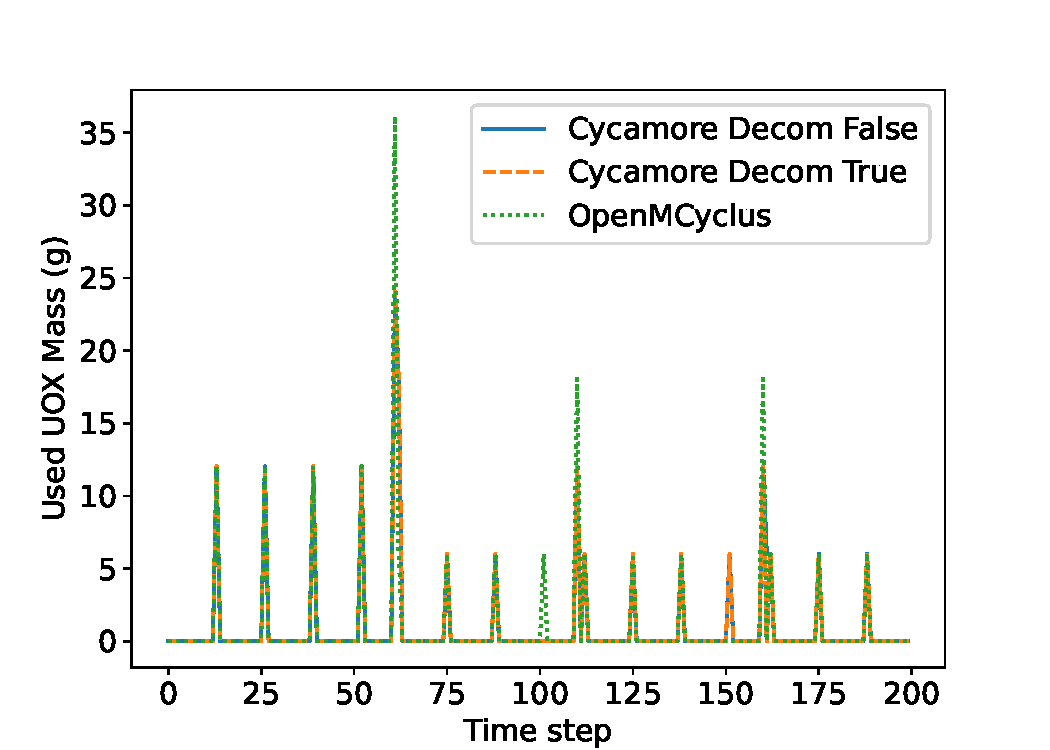
\includegraphics[trim=0 0 30 20,clip,width=\textwidth]{comparison_spentuox.pdf}
        \caption{Spent UOX.}
        \label{fig:comparison_spentuox}
    \end{subfigure}
    \hfill
    \begin{subfigure}[b]{0.48\textwidth}
        \centering
        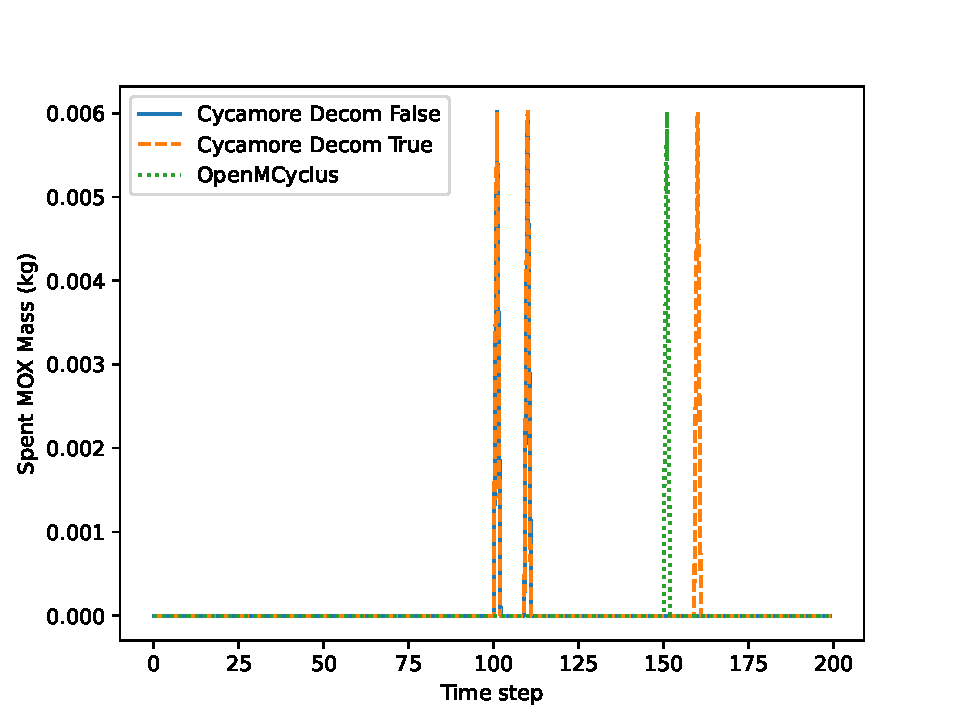
\includegraphics[trim=0 0 30 20,clip,width=\textwidth]{comparison_spentmox.pdf}
        \caption{Spent MOX.}
        \label{fig:comparison_spentmox}
    \end{subfigure}
       \caption{Transactions of the spent fuel commodities from the 
       reactor facilities when defined with each archetype and 
       setting.}
       \label{fig:comparison_spentfuel}
\end{figure}

Finally, Figure \ref{fig:comparison_pu} shows the instantaneous and cumulative 
masses of separated plutonium traded from the separations facility to 
the fuel fabrication facility. The three different scenarios show consistency
in when the separated plutonium is traded: one time step after a spent
\gls{UOX} assembly is traded to the separations facility. However, the 
amount of plutonium traded varies between the three scenarios. The two 
scenarios that use the \Cycamore \texttt{Reactor} show agreement in the 
traded plutonium mass until time step 61, when the first two reactors are
retired. The disagreement between these two scenarios arises from the 
\texttt{decom\_transmute\_all} setting. When set to \texttt{True}, 
all of the assemblies in the core are transmuted upon retirement, 
while when set to \texttt{False} only half of the assemblies are 
transmuted (in this case two of the three assemblies). Therefore, 
when this setting is \texttt{False}, not all of the 
spent fuel assemblies traded away have the spent fuel composition, and 
therefore there is less plutonium in the defined material compositions 
of the spent fuel assemblies than when all of the assemblies are transmuted. 

\begin{figure}
    \centering
    \begin{subfigure}[b]{0.48\textwidth}
        \centering
        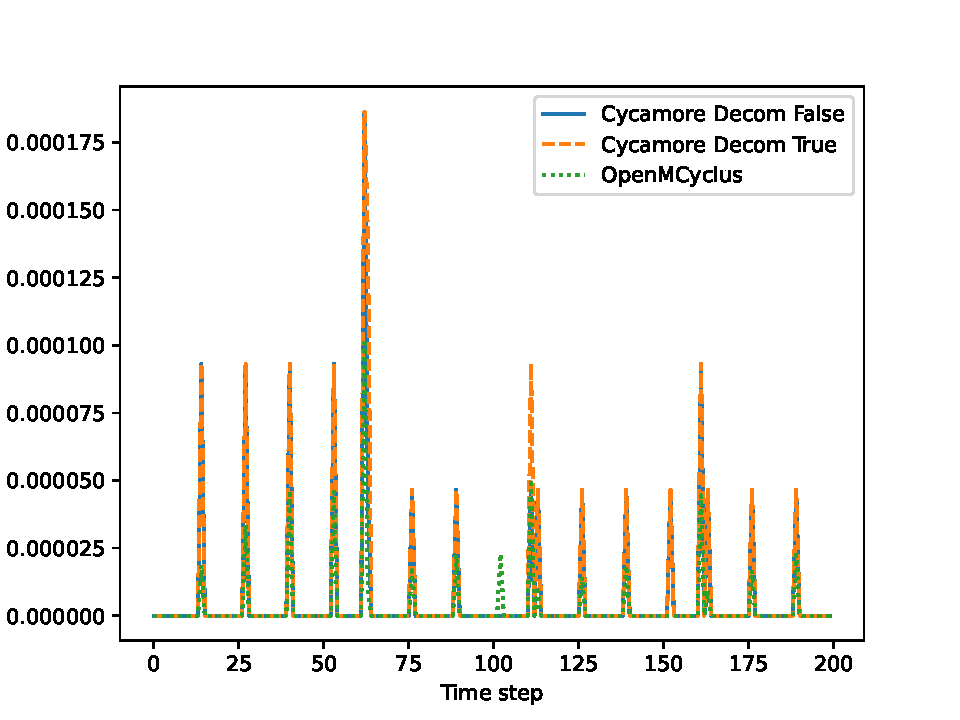
\includegraphics[trim=0 0 30 20,clip,width=\textwidth]{comparison_pu.pdf}
        \caption{Instantaneous plutonium mass}
        \label{fig:comparison_pu_inst}
    \end{subfigure}
    \hfill
    \begin{subfigure}[b]{0.48\textwidth}
        \centering
        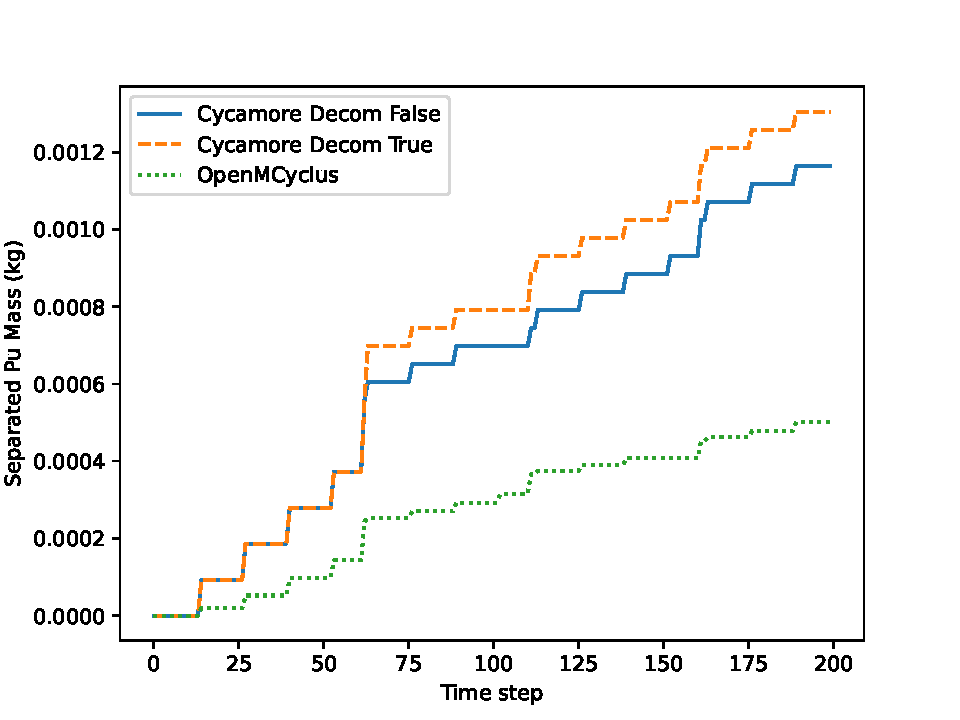
\includegraphics[trim=0 0 30 20,clip,width=\textwidth]{comparison_pu_cumulative.pdf}
        \caption{Cumulative plutonium mass}
        \label{fig:comparison_pu_cumulative}
    \end{subfigure}
       \caption{Transactions of the separated plutonium from the
       separation facility to the fuel fabrication facility, based 
       on the archetype to define the reactor facilities.}
       \label{fig:comparison_pu}
\end{figure}

The differences between the \Cycamore and OpenMCyclus scenarios led 
to the differences in the type of fresh and spent fuel commodities 
traded to and from the reactors. The differences stem 
primarily from the different methodologies in how the assemblies 
are transmuted. For the spent fuel compositions in the cases with the \Cycamore 
\texttt{Reactor}, we depleted an assembly for an entire residence time 
(36 months continuously). However, in OpenMCyclus the fuel is depleted for 
a single cycle at a time (12 months in this case). Therefore, the 
assemblies discharged at the end fo the first two cycles by the 
OpenMCyclus prototypes have not been depleted for the full 36 months 
like they are with the \Cycamore \texttt{Reactor} prototype. To confirm  
that the difference in the time steps of the depletion led to the 
difference in separated plutonium inventory, we temporarily changed
the OpenMCyclus source code to deplete the fuel in a more similar 
manner to that of the \Cycamore \texttt{Reactor}: each assembly was 
depleted for the full 36 month residence time right before being 
discharged. This modification, shown in red in Figure 
\ref{fig:comparison_pu_discharge}, shows that when the assemblies 
are always depleted for the full 36 month duration the 
separated plutonium masses are more consistent with those from 
using the \Cycamore \texttt{Reactor} archetype. The consistency 
between the two archetypes when using the modified OpenMCyclus 
provides confidence in the results of OpenMCyclus when the fuel 
is depleted each cycle instead of upon discharge. 

\begin{figure}
    \centering
    \begin{subfigure}[b]{0.48\textwidth}
        \centering
        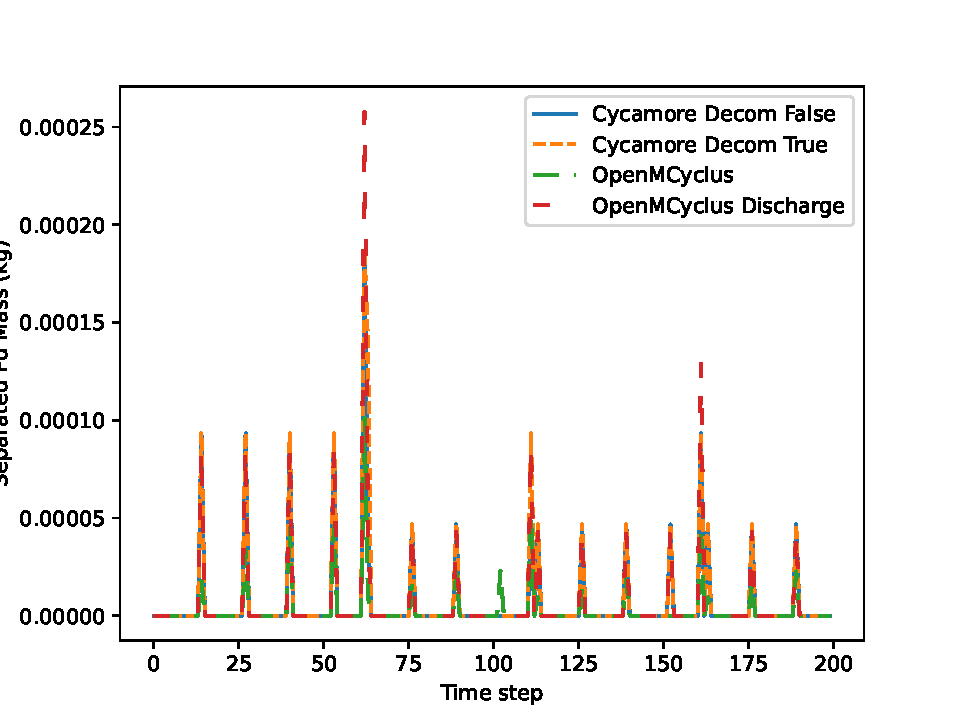
\includegraphics[trim=0 0 30 20,clip,width=\textwidth]{comparison_pu_discharge.pdf}
        \caption{Instantaneous plutonium mass}
        \label{fig:comparison_pu_inst_discharge}
    \end{subfigure}
    \hfill
    \begin{subfigure}[b]{0.48\textwidth}
        \centering
        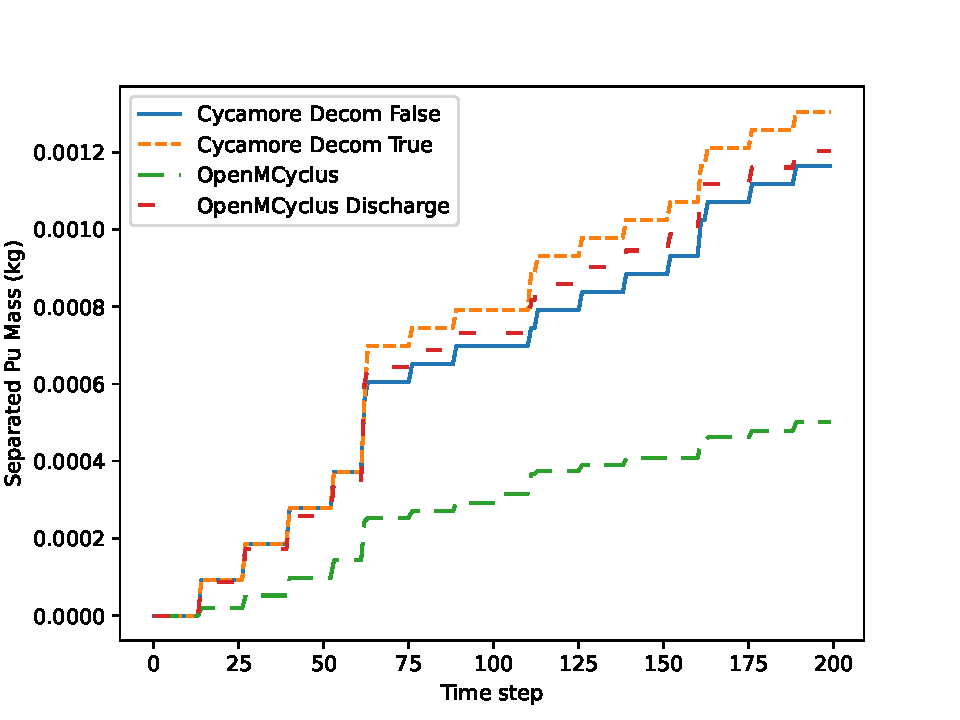
\includegraphics[trim=0 0 30 20,clip,width=\textwidth]{comparison_pu_cumulative_discharge.pdf}
        \caption{Cumulative plutonium mass}
        \label{fig:comparison_pu_cumulative_discharge}
    \end{subfigure}
       \caption{Transactions of the separated plutonium from the
       separation facility to the fuel fabrication facility, based 
       on the archetype to define the reactor facilities.}
       \label{fig:comparison_pu_discharge}
\end{figure}

\section{Calculation of results} \label{sec:results_calc}
The results of each transition scenario modeled include the energy generated, 
the number of advanced reactors deployed, the mass of enriched uranium, 
mass of feed uranium, \gls{SWU} capacity required to produce the enriched 
uranium, and the \gls{SNF} discharged from the reactors. Each of these results 
are obtained from the \Cyclus output file of the simulation. 

The energy generated in each scenario is calculated and directly 
reported by \Cyclus. Each reactor facility is assumed to produce a 
commodity called ``power'', and the total output of each reactor facility 
is reported at each time step that they produce this commodity. 
\Cyclus reports the time step that each facility in the simulation enters 
(commissions) and exits (decommissions) the simulation. Based on 
this information the total number of reactors, advanced reactors, and 
each type of reactor can be determined. 

The other results in this work are calculated based on commodity 
transactions to and from the reactor facilities. The mass of enriched 
uranium is the mass of fuel traded between the enrichment facility and 
the reactors, multiplied by the mass fraction of uranium in the fuel 
form. Multiplying by the mass fraction of uranium means that the other 
fuel components are not included in this mass and the reported mass is 
the product produced by an enrichment facility, $P$ in Eq. 
\ref{eq:enrichment}. This methodology does not account for any 
losses from fuel fabrication.

The feed uranium masses and \gls{SWU} capacity are calculated 
based on the mass of enriched uranium traded to the reactors, using 
Eq. \ref{eq:enrichment}. The natural uranium traded to the enrichment 
facility and the \gls{SWU} capacity of the enrichment facility reported 
by 
\Cyclus are not used because the enrichment facility does not have a 
specified limit on the amount of feed material it can store. Therefore, 
the enrichment facility continuously requests and receives feed 
uranium from the uranium mine without consideration for how much it needs 
to produce the enriched uranium for the reactors. This work does not 
place a limit on the enrichment facility capacity to ensure that the 
reactors are fully fueled and prevent other facility limits to 
influence the reported material demands. 

Finally, in the once through scenarios the mass of \gls{SNF} generated is 
the mass of spent fuel that is 
traded from the reactor facilities to the cooling pools. This mass is the 
entire fuel form, not just the uranium or heavy metal mass in the spent 
fuel, because the entire fuel form must be considered when determining 
disposal needs and options. In the recycling scenarios, the spent fuel 
mass is the mass traded from separations and \gls{MOX} cooling facilities 
to the repository. This change in the calculation of spent fuel mass 
in the recycling scenarios is because not all of the material discharged 
from the reactors is disposed of in these scenarios, and the inclusion of 
reprocessing is captured in this metric. 


\chapter{Once-through transition results} \label{ch:once_through_results}
The once-through transition scenarios are compared on multiple 
criteria: the energy supplied by the reactors, the number of 
advanced reactors deployed, the uranium resources required, the 
amount of \gls{SWU} capacity required to enrich uranium, and the 
mass of \gls{SNF} discharged. Each of these metrics can be used to inform 
policies and decisions of potential deployment schedules and the 
fuel cycle infrastructure required to support the deployment schedule. 

Bachmann et al. \cite{bachmann_enrichment_2021} presents a subset of 
these results for similar scenario definitions, except in that work 
they assumed the 
\glspl{LWR} operate for 60 years if they are not decommissioned before December 
2020. This difference in 
the assumed lifetime of the \glspl{LWR} impacts the energy demand, 
the deployment schedule of advanced reactors, and the material 
requirements of the advanced reactors because a different number of 
\glspl{LWR} are operating when the transition begins. The results of 
Scenario 1 (only \glspl{LWR} with no transition to advanced reactors) 
are presented first. Then, each metric for the transition scenarios are 
presented, first for the the no growth scenarios 
(Scenarios 2-7) then for the 1\% growth scenarios (Scenarios 
8-13).

\section{Scenario 1: LWRs only}\label{sec:scenario1}
Scenario 1 models only the \glspl{LWR} deployed in the United States with no 
prescribed energy demand. This scenario provides insight on historical 
requirements of the nuclear industry as well as future demands if the 
US does not deploy any new reactors and decommissions current reactors at 
their current license expiration. The 
deployment and material requirements of the \glspl{LWR} will be the same 
for each of the other scenarios (Scenarios 2-13). Therefore, analysis 
of the other scenarios will focus on the requirements of 
the advanced reactors deployed. The results of Scenarios 2-13 
are compared with the results of Scenario 1 to provide a comparison 
of material requirements between new and current reactors. 

Figure \ref{fig:energy_reactor1} shows the number of 
reactors deployed in Scenario 1 as a function of time and the energy 
produced by the \glspl{LWR} each year. The energy produced by the 
\glspl{LWR} scales with the number of reactors deployed, as 
one would expect. This scenario deploys a maximum of 109 
\glspl{LWR} at one time, producing 
between 98.18-99.81 GWe-yr, and deploys 92 \glspl{LWR}
when the transition begins in January 2025. The first \gls{LWR} is 
commissioned in August 1967, and all of the \glspl{LWR} are
decommissioned by October 2055. In 2025, the \glspl{LWR} produce 
87.198 GWe-y of energy, which is the basis of the energy demand for 
the other scenarios. 

\begin{figure}[h!]
    \centering
    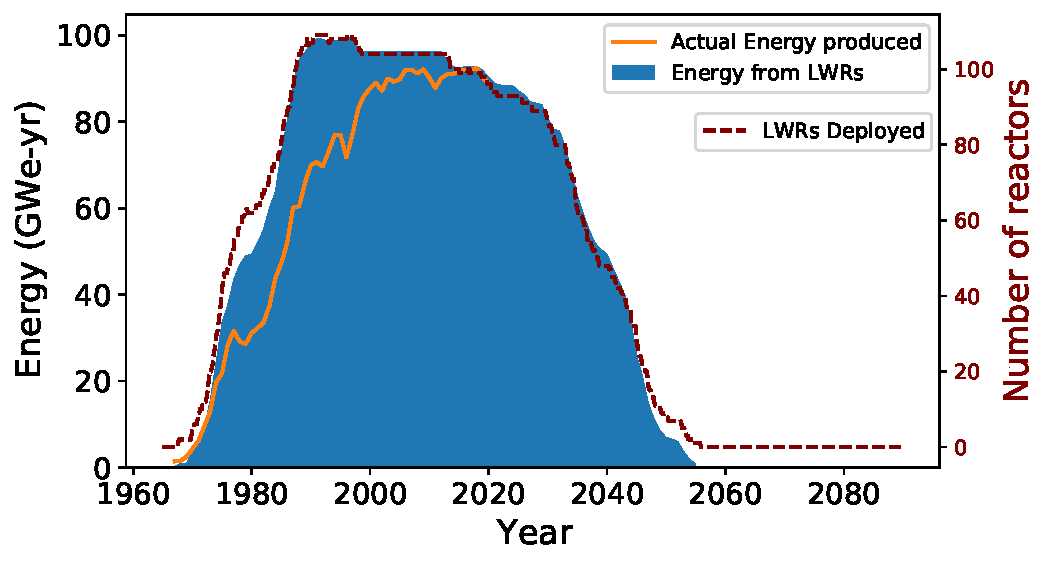
\includegraphics[scale=0.8]{s1_energy_reactors.pdf}
    \caption{Energy supplied by \glspl{LWR} in Scenario 1 during each year of
    the simulation compared to the number of reactors deployed.}
    \label{fig:energy_reactor1}
\end{figure}

Figure \ref{fig:energy_reactor1} also shows historic data of the 
energy generated by nuclear reactors in the US \cite{noauthor_total_2022}.
The energy in this simulation does not always match the historic data 
because of differences in capacity factors. This work assumes that all 
\glspl{LWR} operate at a 92.66\% capacity factor, but the US nuclear fleet
has operated with a wide range of capacity factors because of planned outages 
that last longer than 1 month and unplanned outages. However, 
the difference between the simulation and the historic data are minimal 
during the early 2020's because the capacity factors of the simulation 
and the industry during this time are very similar. 

The mass of enriched uranium sent to the \glspl{LWR} in this scenario (Figure 
\ref{fig:fuel1}) follows the general pattern of the reactor deployment, but with 
more variation between individual time steps. The increased variation between 
time steps is because of the staggering of outages for the reactors, or when 
they receive fuel. Times that receive more fuel correspond with more 
\glspl{LWR} undergoing refueling outages. There are also times with large 
increases in the mass of fuel 
sent to the reactors, such as in 1996, because these times include the deployment 
of a new reactor with a full core of fuel instead of the smaller amount 
required for refueling.

\begin{figure}[h!]
    \centering
    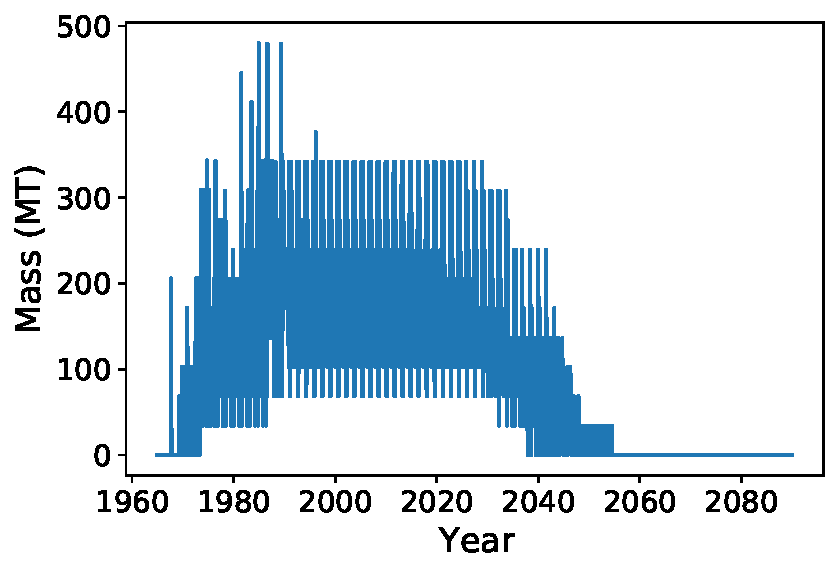
\includegraphics[scale=0.8]{s1_uox.pdf}
    \caption{Mass of enriched uranium supplied to the LWRs in Scenario 1 at each time step.}
    \label{fig:fuel1}
\end{figure}

The maximum amount of enriched uranium sent to the \glspl{LWR} at any one 
time in this scenario is 480.0 MTU, which occurs in the 1980s. The 
average mass of enriched uranium sent to 
\glspl{LWR} while they are deployed (1967-2055) is 135.65 MTU/month. The average 
mass of 
enriched uranium sent to the \glspl{LWR} between when they are first deployed 
and 2025 is 164.57 MTU/month. This average is larger than what is reported in 
\cite{bachmann_enrichment_2021} because the average reported by 
Bachmann et al. accounts for the time before the \glspl{LWR} are  
deployed while the average reported here does not. The average mass of 
uranium sent to \glspl{LWR} between 2025-2055, from the start of the transition 
to when they are all decommissioned is 81.48 MTU/month. Comparing the averages 
shows that the vast majority of enriched uranium is sent to the \glspl{LWR} 
before 2025, which matches with the decline in the number of \glspl{LWR} 
deployed after 2020. After 2025, a cumulative total of 29,985 MTU is 
sent to the \glspl{LWR},
which is less than the cumulative mass reported in \cite{bachmann_enrichment_2021}
because Bachmann et al. assumed that all \glspl{LWR} would operate for 60 years, 
which is longer than the assumed operating time for some \glspl{LWR} in 
this work. This scenario requires a cumulative total of 143,377 MT of enriched uranium.

The next metric of interest is the mass of natural uranium 
required as feed material to produce the enriched uranium for the 
reactors, shown in Figure \ref{fig:feed1}. The mass of feed uranium 
is about an order of magnitude larger than the mass of the enriched uranium. 
Scenario 1 requires a maximum of 2850 MT of 
feed uranium at one time and an average of 1,088 MT/month of natural uranium 
when \glspl{LWR} are deployed. Before 2025, this scenario requires an average of 
1,320 MTU/month of natural uranium, and requires an average of 653.8 MTU/month 
after 2025. In total, the \glspl{LWR} require 1,150,385 MT of feed uranium.

\begin{figure}[h!]
    \centering
    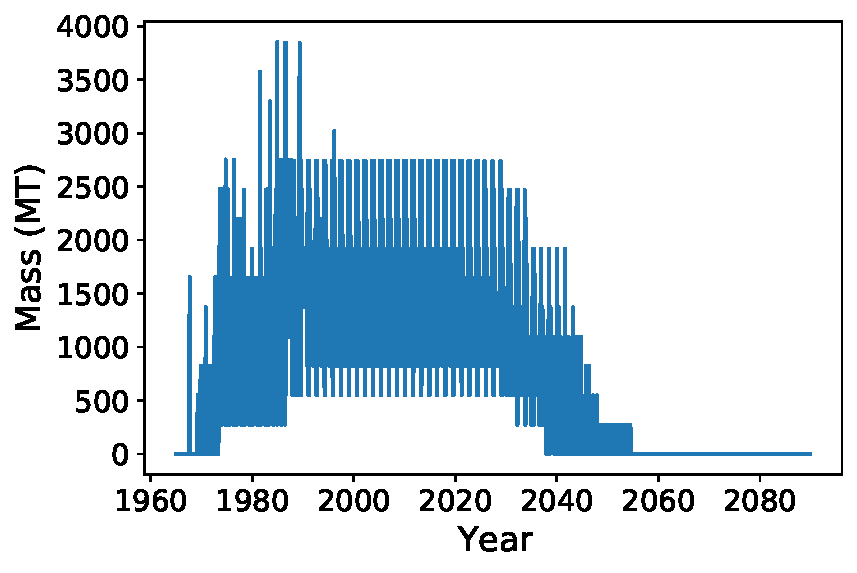
\includegraphics[scale=0.8]{s1_feed.pdf}
    \caption{Mass of natural uranium required to produce fuel for the LWRs at each 
    time step in Scenario 1.}
    \label{fig:feed1}
\end{figure}

Next is the \gls{SWU} capacity required 
to produce the enriched uranium for the \glspl{LWR}, 
shown in Figure \ref{fig:swu1}. This scenario requires a maximum of 3,470 
MT-SWU to 
enrich the uranium sent to the reactors at one time step and an average of 
981 MT-SWU/month to enrich all of the uranium sent to 
the \glspl{LWR} when they are deployed. An average of 
1189 MT-SWU/month is required to produce the enriched uranium 
for \glspl{LWR} between their initial deployment and 2025, and 
589.1 MT-SWU/month is needed to produce the 
enriched uranium sent to \glspl{LWR} between 2025 and 2055. The values 
reported here are different than what Bachmann et al. \cite{bachmann_enrichment_2021}
reports for a few different reasons. The first reason is that these results  
consider only
the time steps in which the \glspl{LWR} are deployed (1967-2055) while Bachmann et al. 
considers all time steps (1965-2090). The other reason
is the use of different enrichment levels for the \gls{LWR} fuel. 
Bachmann et al. assumes an enrichment of 4.5\% while this work assumes 4.3\%
$^{235}$U enrichment for \gls{LWR} fuel. 


\begin{figure}[h!]
    \centering
    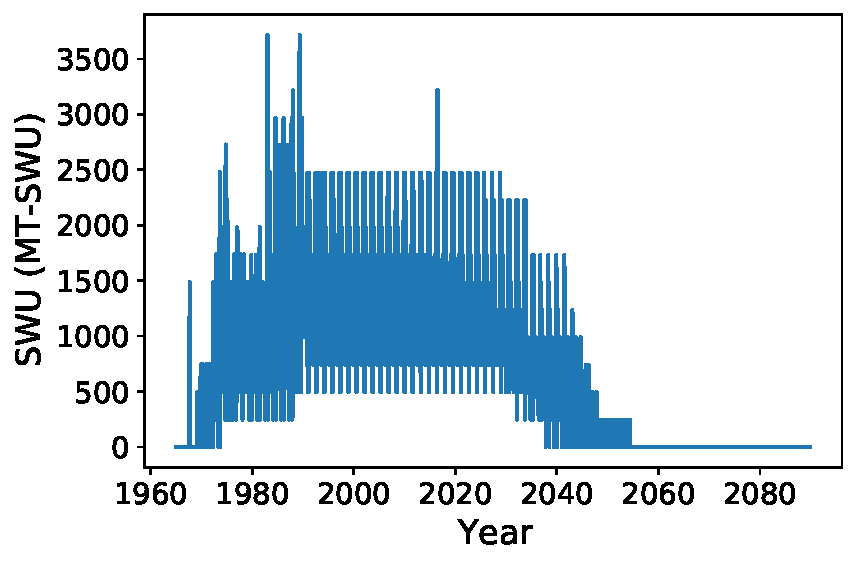
\includegraphics[scale=0.8]{s1_swu.pdf}
    \caption{SWU capacity required to enrich the uranium sent to LWRs at each time step in Scenario 1.}
    \label{fig:swu1}
\end{figure}

The last metric is the \gls{SNF} discharged from the reactors as a function of
time (Figure \ref{fig:waste1}). The \glspl{LWR} discharge a maximum of 411.1 MT 
of spent fuel in one time step and an average of 130.0 MT/month when they are 
deployed. Between the first \gls{LWR} deployment and 2025 the \glspl{LWR} 
discharge an average of 149.1 MTU/month, and an average of 94.27 MT/month  
between 2025-2055. The \glspl{LWR} discharge a total of 137,479 MT of \gls{SNF} 
in Scenario 1. 

\begin{figure}[h!]
    \centering
    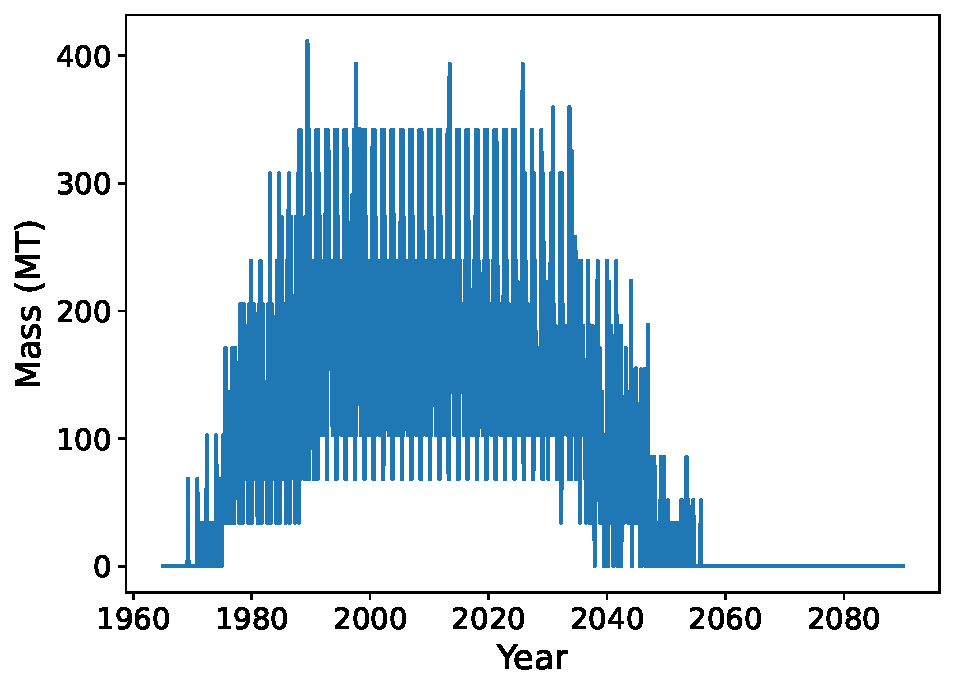
\includegraphics[scale=0.8]{s1_waste.pdf}
    \caption{Mass of spent fuel discharged from the reactors in Scenario 1 as a function of time.}
    \label{fig:waste1}
\end{figure}

Table \ref{tab:s1_results} summarizes all of the material needs of Scenario 1. 

\begin{table}[h!]
    \centering
    \caption{Summary of material needs for Scenario 1. Averages listed 
    are for the duration that \glspl{LWR} are deployed (1967-2055).}
    \label{tab:s1_results}
    \begin{tabular}{c c c c c}
        \hline 
        Metric & Average & Cumulative & Maximum & Units \\\hline
        Uranium mass & 135.6 & 143,377 & 480.0 & MT \\
        Feed uranium mass & 1088 & 1,150,385 & 3850 & MT \\
        SWU Capacity & 980.7 & -- & 3470 & MT-SWU \\
        Waste discharged & 130.0 & 137,479 & 411 & MT \\
        \hline        
    \end{tabular}
\end{table}

\section{Energy Generated} \label{sec:energy}
This section reports and compares the energy produced in the no growth and 
1\% growth transition scenarios to the energy demand. This result 
considers the energy produced by \glspl{LWR} and advanced reactors, 
and compares the different scenarios based on any under- or 
over-supply of energy present. 

\subsection{No growth scenarios}
The energy demand in the no growth scenarios (Scenarios 2-7) is a constant
87.198 GWe-yr, based on the energy supplied by the reactors in Scenario 1
in 2025. The energy produced in each of these scenarios meets or exceeds the 
demand, as Figure \ref{fig:nogrowth_energy} shows. There is little variation 
in the amount of energy produced in each of these scenarios because refueling 
outages are not explicitly modeled. All of the scenarios have an oversupply 
of power in 2025, up to 0.2 GWe-yr (Table \ref{tab:nogrowth_energy}), before 
dropping to a value closer to the energy demand. This initial oversupply 
of 0.2 GWe-yr is a result of the energy demand being set based on the average 
amount of energy the \glspl{LWR} supply over 2025. The \glspl{LWR} provide 
slightly more than the demand in the first few months of 2025, and the 
demand is met through \glspl{LWR} and advanced reactors in the later 
months of the year. 

\begin{figure}[h!]
    \centering
    \begin{subfigure}{0.45\textwidth}
        \centering
        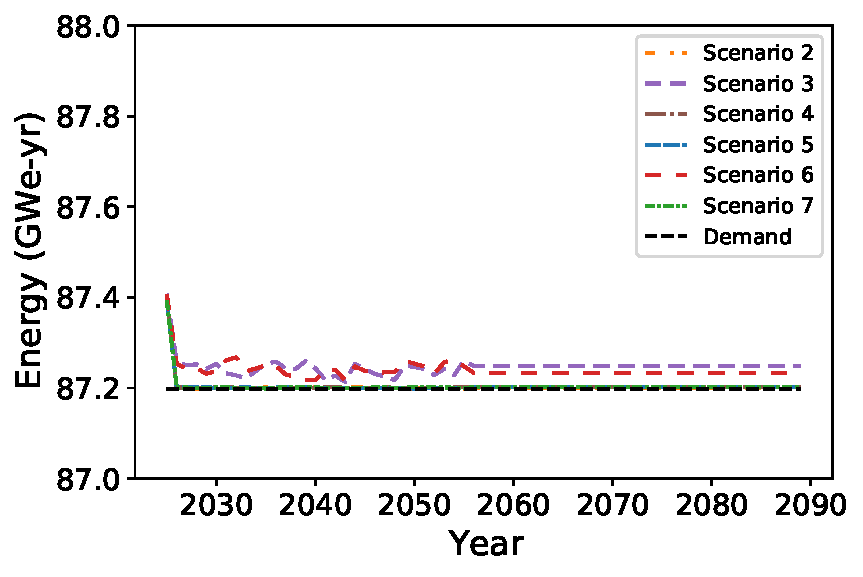
\includegraphics[width=\textwidth]{nogrowth_energy_after_2025.pdf}
        \caption{Annual energy produced compared to demand for Scenarios 2-7
        between 2025-2090.}
        \label{fig:nogrowth_energy_after_2025}
    \end{subfigure}
    \hfill
    \begin{subfigure}{0.45\textwidth}
        \centering
        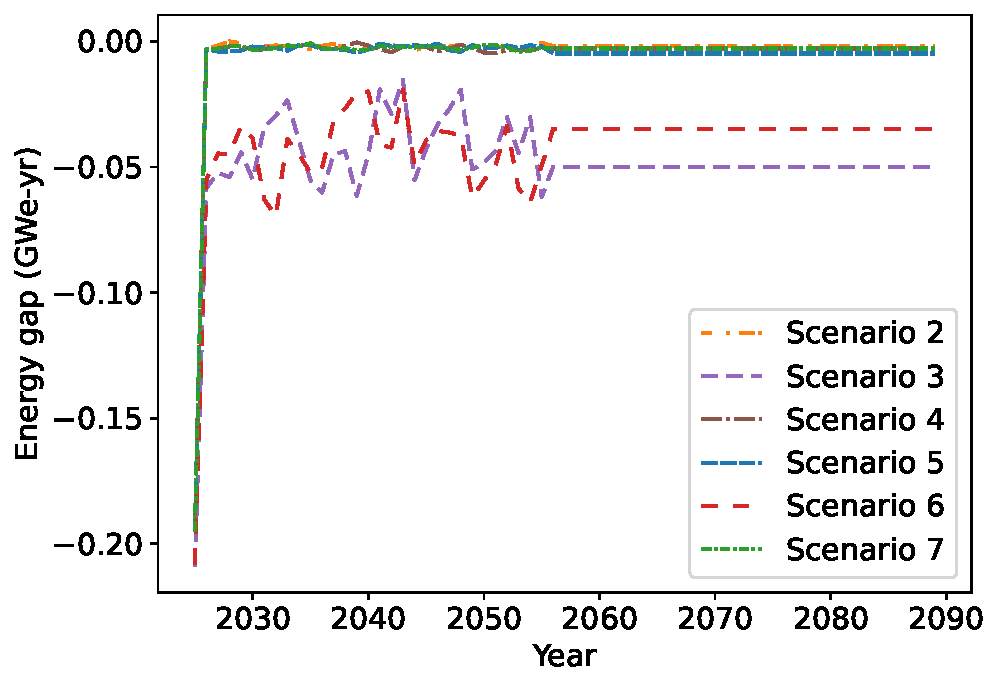
\includegraphics[width=\textwidth]{nogrowth_energy_gap.pdf}
        \caption{Gap between energy demand and energy produced by reactors 
        in Scenarios 2-7 between 2025-2090. Positive values indicate an 
        undersupply of energy and negative values represent an 
        oversupply of energy.}
        \label{fig:nogrowth_energy_gap}
    \end{subfigure}
       \caption{Annual energy produced compared to demand in Scenarios 2-7.}
       \label{fig:nogrowth_energy}
\end{figure}

\begin{table}[h!]
    \centering
    \caption{Maximum undersupply and oversupply of energy in Scenarios 2-7.}
    \label{tab:nogrowth_energy}
    \begin{tabular}{c c c}
        \hline 
        Scenario & Maximum oversupply (GWe-yr) & Maximum undersupply (GWe-yr) \\
        \hline 
        2 & 0.195 & 0.000 \\
        3 & 0.209 & 0.000 \\
        4 & 0.195 & 0.000 \\
        5 & 0.195 & 0.000 \\
        6 & 0.208 & 0.000 \\
        7 & 0.195 & 0.000 \\
        \hline
        
    \end{tabular}
\end{table}

Scenarios 3 and 6 produce an 
oversupply of energy because these scenarios only deploy the Xe-100 and VOYGR,
which have a larger power output than the \gls{MMR}. Therefore,
their deployment can't be used to fine-tune meeting an energy demand. The oversupply 
of energy in each of these scenarios ranges between 15-69 MWe-yr, which is less 
than the power output of the Xe-100 and VOYGR and demonstrates the round-up 
aspect of the deployment scheme in this work. 

\subsection{1\% growth scenarios}
In the 1\% growth scenarios, the energy demand is always 
met or exceeded, as shown in Figure \ref{fig:1percent_energy}. There is an 
initial oversupply of energy, which is consistent with the 
results energy produced in the no growth scenarios. The 
maximum oversupply of energy among the 1\% growth scenarios 
(Table \ref{tab:1percent_energy}) is 0.436 GWe-yr, which is more 
than the maximum oversupply of energy in the no growth 
scenarios. 

\begin{figure}[h!]
    \centering
    \begin{subfigure}[b]{0.45\textwidth}
        \centering
        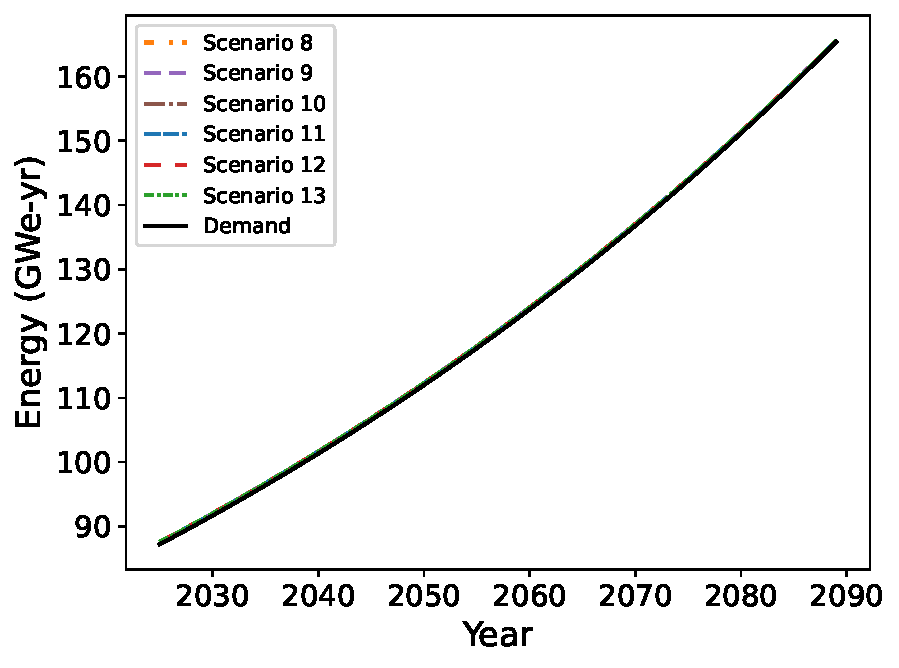
\includegraphics[width=\textwidth]{1percent_energy_after_2025.pdf}
        \caption{Annual energy produced compared to demand for Scenarios 8-13
        between 2025-2090.}
        \label{fig:1percent_energy_after_2025}
    \end{subfigure}
    \hfill
    \begin{subfigure}[b]{0.45\textwidth}
        \centering
        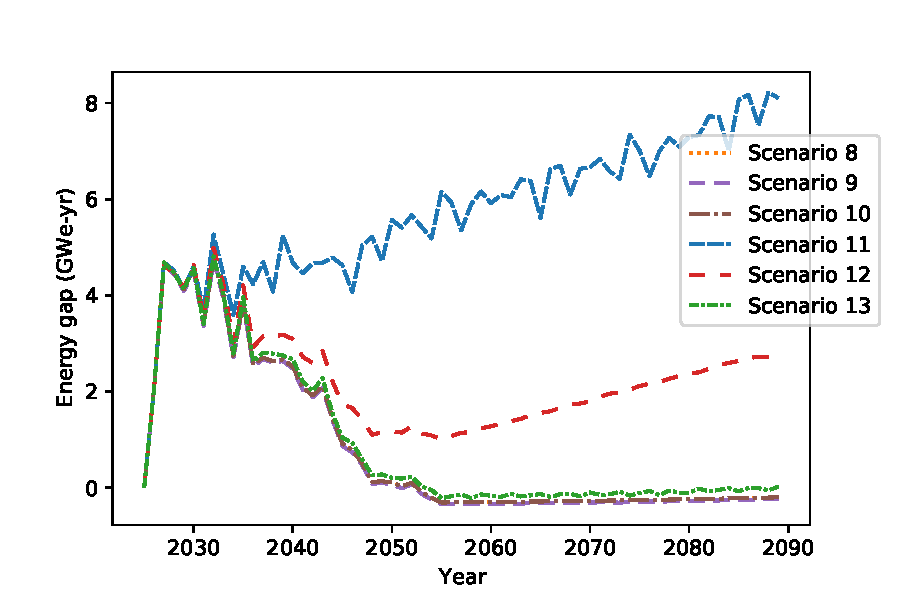
\includegraphics[width=\textwidth]{1percent_energy_gap.pdf}
        \caption{Gap between energy demand and energy produced in Scenarios 8-13
        between 2025-2090. Positive values represents an undersupply of energy 
        and negative values represents an oversupply of energy. }
        \label{fig:1percent_energy_gap}
    \end{subfigure}
       \caption{Annual energy produced compared to demand in Scenarios 8-13.}
       \label{fig:1percent_energy}
\end{figure}

\begin{table}[h!]
    \centering
    \caption{Maximum undersupply and oversupply of energy in Scenarios 8-13.}
    \label{tab:1percent_energy}
    \begin{tabular}{c c c}
        \hline 
        Scenario & Maximum oversupply (GWe-yr) & Maximum undersupply (GWe-yr) \\
        \hline 
        8 & 0.406 & 0.000 \\
        9 & 0.424 & 0.000 \\
        10 & 0.406 & 0.000 \\
        11 & 0.406 & 0.000 \\
        12 & 0.436 & 0.000 \\
        13 & 0.406 & 0.000 \\
        \hline
    \end{tabular}
\end{table}

There is consistency in the amount of energy oversupply between scenarios that deploy similar reactors.
All of the scenarios that deploy \glspl{MMR} (Scenarios 8, 10, 11, and 13) have the 
same over maximum oversupply of energy, and the other two scenarios 
have similar maximum oversupplies of energy. This consistency 
is a result of the deployment scheme deploying the reactor with the 
smallest power output last to meet any remaining demand. 

\section{Reactor deployment}
The different power output of each advanced reactor leads to different 
requirements in the number of advanced reactors deployed in each transition 
scenario. 
This section compares the scenarios on the number of advanced reactors 
built. This metric takes two 
different forms: the number of reactors that are in the simulation at 
one time and the number of reactors that are built (enter the simulation)
in a single time step. These metrics combined provide insight into the 
number of reactors needed and the rate at which to build them. 

\subsection{No growth scenarios} \label{sec:nogrowth_reactors}
Advanced reactors are first deployed in September 2025 for Scenario 2-7, 
9 months after the transition start time. The advanced reactor initial 
deployment time is more than six years earlier than the initial deployment 
time reported for no growth scenarios in the work by Bachmann et al.  
\cite{bachmann_enrichment_2021}. The differences in deployment times results 
from different deployment schemes (Bachmann et al. used the \Cycamore 
\texttt{ManagerInst} institution to deploy advanced reactors to match installed 
capacity to a demand in energy generation), different power output from 
the \gls{MMR} and Xe-100, and a different energy demand 
(resulting from different assumptions of how long \glspl{LWR} operate). 

The number of reactors deployed varies based on 
the reactors deployed in each scenario and scales with the power output of 
each type of reactor, as shown in Figure \ref{fig:nogrowth_reactors}. Scenario
2 requires the most reactors, requiring 17,440 reactors at one time, 
because the \gls{MMR} has the smallest power output of the reactors 
considered in this work. Scenario 3 requires the fewest 
advanced reactors (1148) because this scenario only deploys the Xe-100,
which has the largest power output. 

\begin{figure}[h!]
    \centering
    \begin{subfigure}[b]{0.45\textwidth}
        \centering
        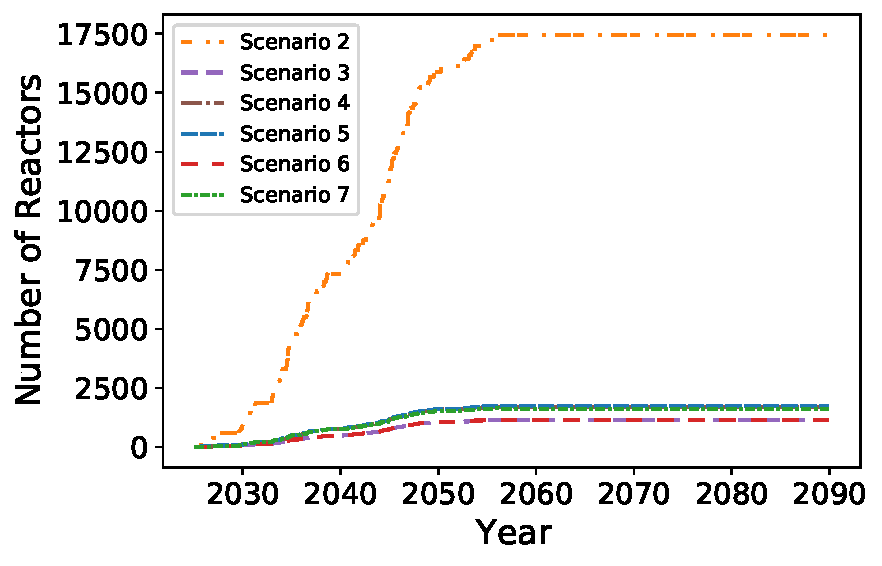
\includegraphics[width=\textwidth]{nogrowth_reactors.pdf}
        \caption{Total number of advanced reactors deployed at 
        each time step in Scenarios 2-7 between 2025-2090.}
        \label{fig:nogrowth_reactors_all}
    \end{subfigure}
    \hfill
    \begin{subfigure}[b]{0.45\textwidth}
        \centering
        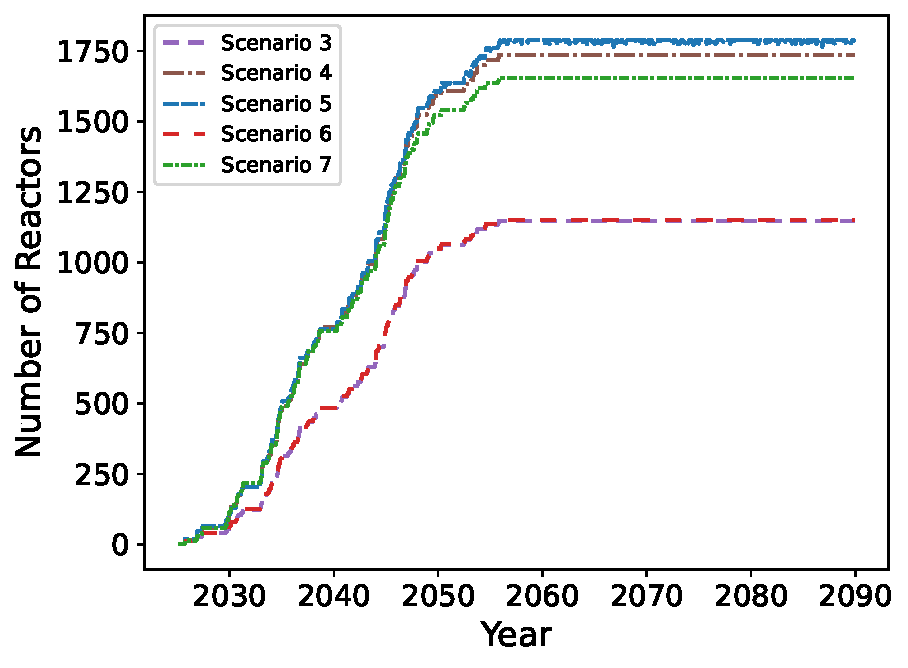
\includegraphics[width=\textwidth]{nogrowth_reactors_3-7.pdf}
        \caption{Total number of advanced reactors deployed at 
        each time step in Scenario 3-7 between 2025-2090.}
        \label{fig:nogrowth_reactors_3-7}
    \end{subfigure}
       \caption{Number of advanced reactors deployed at each time step 
       for Scenarios 2-7. The figures begin at 2025, because no advanced 
       reactors are deployed before then. In the right figure Scenario 
       2 is removed to highlight the trends in the other scenarios.}
       \label{fig:nogrowth_reactors}
\end{figure}

\begin{table}[h!]
    \centering 
    \caption{Maximum number of reactors deployed at one time in 
    Scenarios 2-7.}
    \label{tab:reactors_nogrowth}
    \begin{tabular}{c c c c c}
        \hline
        Scenario & \glspl{MMR} [\#] & Xe-100s [\#] & VOYGRs [\#] 
        & Total [\#]\\\hline
        2 & 17,440 & - & - & 17,440\\
        3 & - & 1,148 & - & 1,148\\
        4 & 629 & 1,106 & - & 1,735\\
        5 & 636 & - & 1,151 & 1,787\\
        6 & - & 1,070 & 81 & 1,151\\
        7 & 542 & 1,105 & 7 & 1,654\\
        \hline
    \end{tabular}
\end{table}

All of the scenarios have a constant number of advanced reactors 
deployed starting in October 2055 because all of the \glspl{LWR} are 
decommissioned by this time and the deployment scheme replaces advanced
reactors with a reactor of the same design. The number of Xe-100s and VOYGRs combined 
in each scenario is similar, about 1,100, because these two reactor 
designs have similar power outputs (80 MWe and 77 MWe, respectively). 
Therefore, the deployment of one over the other does 
not greatly affect the total number of reactors deployed to meet the 
energy demand. However, 
deploying them in tandem reduces the number of \glspl{MMR} deployed
(Scenarios 4 and 5 compared with Scenario 7). 

Scenarios 4, 6, and 7 primarily deploy Xe-100s and Scenario 5 primarily deploys 
VOYGRs as a result of the deployment scheme used in this work. The Xe-100 and 
VOYGR have the largest power output of the reactors deployed in each of those 
scenarios, and are therefore preferentially deployed in each of these scenarios.
This preferential deployment leads to these reactors supplying most of 
the energy in each scenario.  

In addition to the total number of advanced reactors deployed 
at each time, the maximum number of each advanced reactor deployed in a 
single time step is reported in Table 
\ref{tab:reactors_added_nogrowth}. This information provides insight 
into the speed at which new reactors must be built. For scenarios with 
multiple advanced reactors, the numbers reported do not necessarily occur 
in the same time step. Scenario 2 requires 
the largest number of reactors to be deployed at a single time, because 
the \gls{MMR} has the smallest power output. Scenarios 3 and 
6 deploy the fewest reactors in 
a single time step, based on the total column of Table 
\ref{tab:reactors_added_nogrowth}, because of the large power output from 
the Xe-100 and VOYGR. 

\begin{table}[h!]
    \centering 
    \caption{Maximum number of reactors added to the simulation at a 
    single time step in Scenarios 2-7.}
    \label{tab:reactors_added_nogrowth}
    \begin{tabular}{c c c c c}
        \hline
        Scenario & \glspl{MMR} [\#]& Xe-100s [\#]& VOYGRs [\#]
        & Total[\#]\\\hline
        2 & 856 & - & - & 856\\
        3 & - & 46 & - & 46\\
        4 & 16 & 46 & - & 52\\
        5 & 24 & - & 47 & 66\\
        6 & - & 45 & 1 & 46\\
        7 & 16 & 46 & 1 & 52\\
        \hline
    \end{tabular}
\end{table}

\subsection{1\% growth scenarios} \label{sec:1percent_reactors}
All of the 1\% growth scenarios deploy advanced reactors beginning 
in May 2027, which is 32 months (almost three years) before their initial 
deployment reported by Bachmann et al. for a 1\% growth transition 
\cite{bachmann_enrichment_2021}.

Transitioning to only the 
\gls{MMR} (Scenario 8) requires the largest number of reactors, and 
transitioning to only the Xe-100 (Scenario 9) requires the fewest 
number of advanced reactors (Figure \ref{fig:1percent_reactors}, Table 
\ref{tab:reactors_1percent}). Scenarios 10 and 13 have similar numbers of 
reactors deployed, as do Scenarios 9 and 12, because these pairing differ 
by the inclusion of the VOYGR which has a similar power output to the 
Xe-100. 
Compared with the no growth scenarios, \glspl{MMR} are a greater 
fraction of the total number of reactors deployed when they are deployed 
with the other reactors (Scenarios 10, 11, and 13). This increase is 
because early in the transition, the growth of the energy demand 
changes in increments smaller than the power output of the Xe-100 and 
VOYGR. Therefore, the deployment scheme of this work dictates the 
deployment of \glspl{MMR} to fulfill the unmet demand.

\begin{figure}[h!]
    \centering
    \begin{subfigure}[b]{0.45\textwidth}
        \centering
        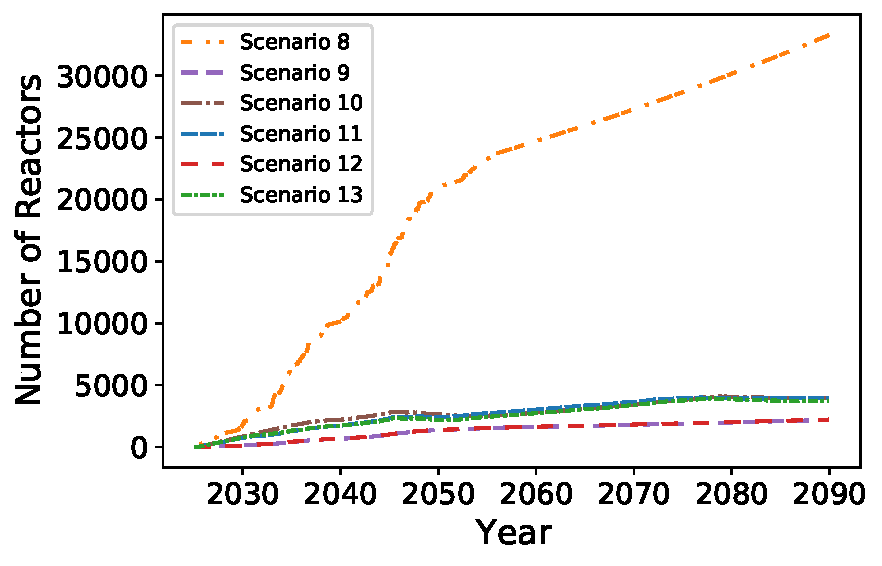
\includegraphics[width=\textwidth]{1percent_reactors.pdf}
        \caption{Total number of advanced reactors deployed at 
        each time step in Scenarios 8-13 between 2025-2090.}
        \label{fig:1percent_reactors_all}
    \end{subfigure}
    \hfill
    \begin{subfigure}[b]{0.45\textwidth}
        \centering
        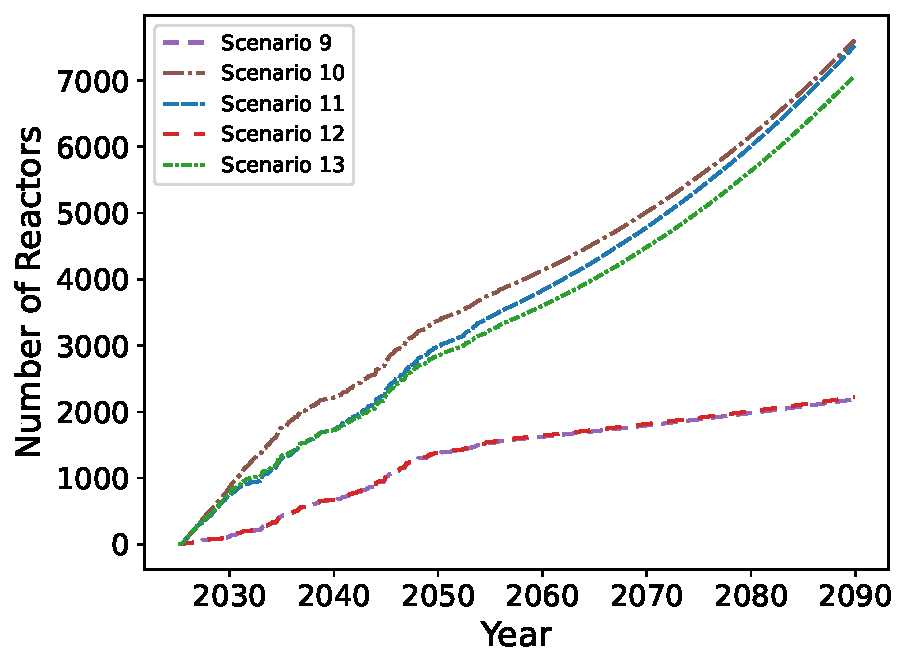
\includegraphics[width=\textwidth]{1percent_reactors_9-13.pdf}
        \caption{Total number of advanced reactors deployed at 
        each time step in Scenario 9-13 between 2025-2090.}
        \label{fig:1percent_reactors_9-13}
    \end{subfigure}
       \caption{Number of advanced reactors deployed at each time step 
       for Scenarios 8-13. The figures begin at 2025, because no advanced 
       reactors are deployed before then. In the right figure Scenario 
       8 is removed to help highlight the trends in the other scenarios.}
       \label{fig:1percent_reactors}
\end{figure}

\begin{table}
    \centering 
    \caption{Maximum number of advanced reactors deployed in Scenarios 8-13.}
    \label{tab:reactors_1percent}
    \begin{tabular}{c c c c c}
        \hline
        Scenario & \glspl{MMR} [\#]& Xe-100s [\#]& VOYGRs [\#] 
        & Total [\#]\\\hline
        8 & 33,265 & - & - & 33,265\\
        9 & - & 2,189 & - & 2,189 \\
        10 & 5,798 & 1,807 & - & 7,605\\
        11 & 5,627 & - & 1,893 & 7,520\\
        12 & - & 1,420 & 801 & 2,221\\
        13 & 5,228 & 1,809 & 37 & 7,704\\
        \hline
    \end{tabular}
\end{table}

The number 
of reactors deployed in the simulation increases with time, 
partly because of the growth in the energy demand and partly 
because of the deployment scheme. The deployment scheme 
dictates that the largest reactor is preferentially deployed to 
meet unmet energy demand. This unmet energy demand is determined 
after decommissioned advanced reactors are replaced with an 
equal number of the same type of advanced reactor. The \gls{MMR} 
has the shortest lifetime, in addition to the smallest power 
output. Therefore, the \glspl{MMR} in the scenarios are replaced with more 
\glspl{MMR}, instead of potentially being replaced with a larger 
reactor if there is enough unmet demand in the time step from 
\gls{MMR} decommissioning or demand growth. 
This aspect of the deployment scheme artificially 
inflates the number of \glspl{MMR} deployed in each scenario, 
which leads to the \glspl{MMR} having a larger effect on the 
material requirements of each scenario. 

Regarding the rate of reactor deployment, Scenario 8 deploys the most 
reactors in a single time step (Table 
\ref{tab:reactors_added_1percent}), with 936 \glspl{MMR} deployed at once. 
Scenario 13 requires the next largest number of reactors deployed in 
a single time step, 58 total advanced reactors built.
The maximum number of Xe-100s and VOYGRs deployed in a single time 
step in the 1\% growth scenarios are similar to the numbers required 
for the no growth scenarios. But the number of \glspl{MMR} 
deployed for a single time step are at least twice the numbers 
for the no growth scenarios. The increase in the number of 
\glspl{MMR} highlights to \glspl{MMR} providing an inflated 
share of the energy demand in the 1\% growth scenarios. 

\begin{table}
    \centering 
    \caption{Maximum number of advanced reactors deployed in a single 
    time step for Scenarios 8-13.}
    \label{tab:reactors_added_1percent}
    \begin{tabular}{c c c c c}
        \hline
        Scenario & \glspl{MMR} [\#] & Xe-100s [\#] & VOYGRs [\#] 
        & Total [\#]\\\hline
        8 & 936 & - & - & 936\\
        9 & - & 47 & - & 47\\
        10 & 49 & 47 & - & 56\\
        11 & 49 & - & 49 & 56\\
        12 & - & 47 & 3 & 48\\
        13 & 46 & 47 & 1 & 58\\
        \hline
    \end{tabular}
\end{table}

\section{Uranium resources}
This metric considers  
both the mass of enriched uranium and the mass of natural uranium feed 
required by each scenario. The feed uranium masses 
considered are the masses needed at an enrichment facility,
and does not account for any process losses during a milling process 
or the grade of the uranium ore. Therefore, the values reported are 
not the same as what would need to be mined. Additionally, the 
enriched uranium masses reported do not account for 
any fuel fabrication losses, which others have previously assumed to 
be 0.1\% \cite{wigeland_nuclear_2014}. Using these assumptions 
still yields reasonable estimates of the uranium resources 
required in each scenario. 

The masses of uranium resources are divided into four 
different metrics: the average monthly mass of uranium to supply all 
advanced reactors, the average monthly mass of \gls{HALEU}, the 
maximum mass of uranium required by all advanced 
reactors in a single time step, and the cumulative mass required by
advanced reactors in the 
scenario. Each of these metrics provide information 
on how to design facilities, such as the average facility capacity 
required to meet the average demand and peaks in demand. The monthly 
averages are calculated beginning in January 2025, 
when the transition begins but not when the advanced reactors 
are first deployed. Therefore, the reported averages are slightly lower 
than if they were calculated starting at the advanced reactor deployment 
time. This reporting methodology provides an average for if 
facilities are built to support the front-end of the \gls{NFC} starting 
in January 2025. Additionally, these metrics do not account for any 
extra fuel assemblies or \gls{TRISO} pebbles kept on site as 
reserve fuel. 

\subsection{No growth scenarios}
\subsubsection{Enriched uranium}
The mass of enriched uranium sent to reactors (Fig. \ref{fig:nogrowth_uranium})
varies based on the advanced reactors deployed in the scenario. 
Scenario 5 has the largest average mass of enriched uranium sent to 
reactors each month, followed by Scenario 2 (Table 
\ref{tab:nogrowth_uranium}). 
Scenario 2 also requires the largest mass of enriched uranium sent 
to advanced reactors at one time, followed by Scenario 5.
Scenario 3 requires the smallest average 
mass of enriched uranium. Scenarios 3, 4, and 7 
have similar monthly averages for enriched uranium mass. All of the 
scenarios require a smaller 
average mass of enriched uranium than the \glspl{LWR} before 2025. 

\begin{figure}[h!]
    \centering
    \begin{subfigure}[b]{0.45\textwidth}
        \centering
        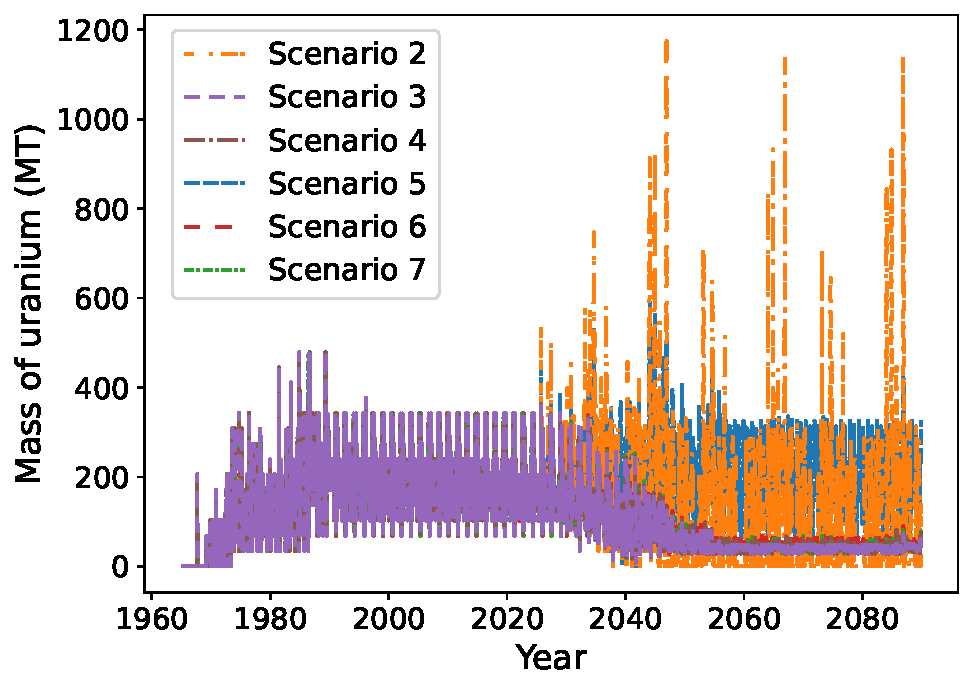
\includegraphics[width=\textwidth]{nogrowth_uranium.pdf}
        \caption{Monthly mass sent to all reactors 
        between 1965-2090.}
        \label{fig:nogrowth_all_uranium}
    \end{subfigure}
    \hfill
    \begin{subfigure}[b]{0.45\textwidth}
        \centering
        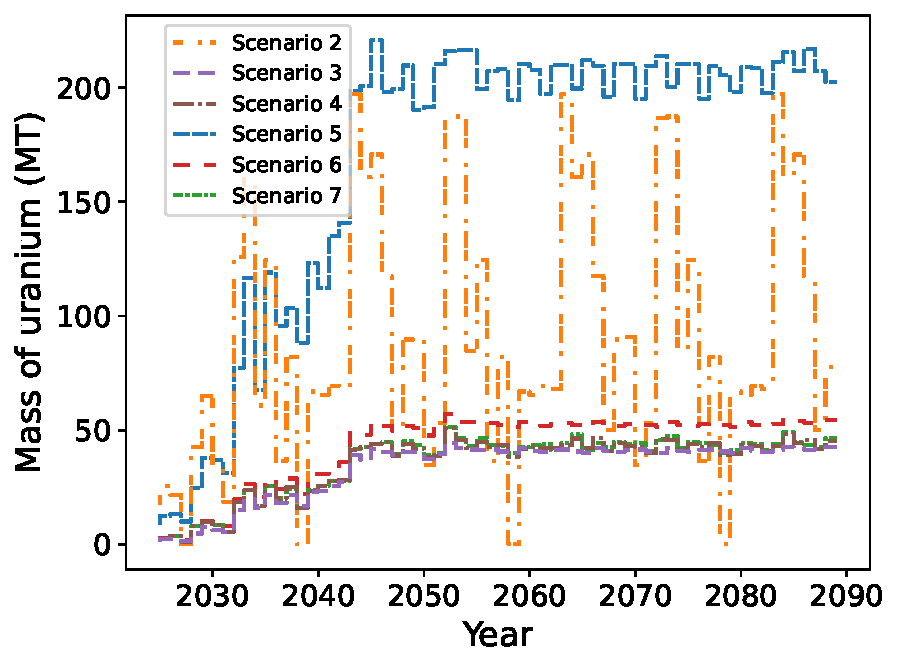
\includegraphics[width=\textwidth]{nogrowth_AR_uranium.pdf}
        \caption{Annual average mass sent to 
        advanced reactors between 2025-2090.}
        \label{fig:nogrowth_AR_uranium}
    \end{subfigure}
    \begin{subfigure}[b]{0.45\textwidth}
        \centering
        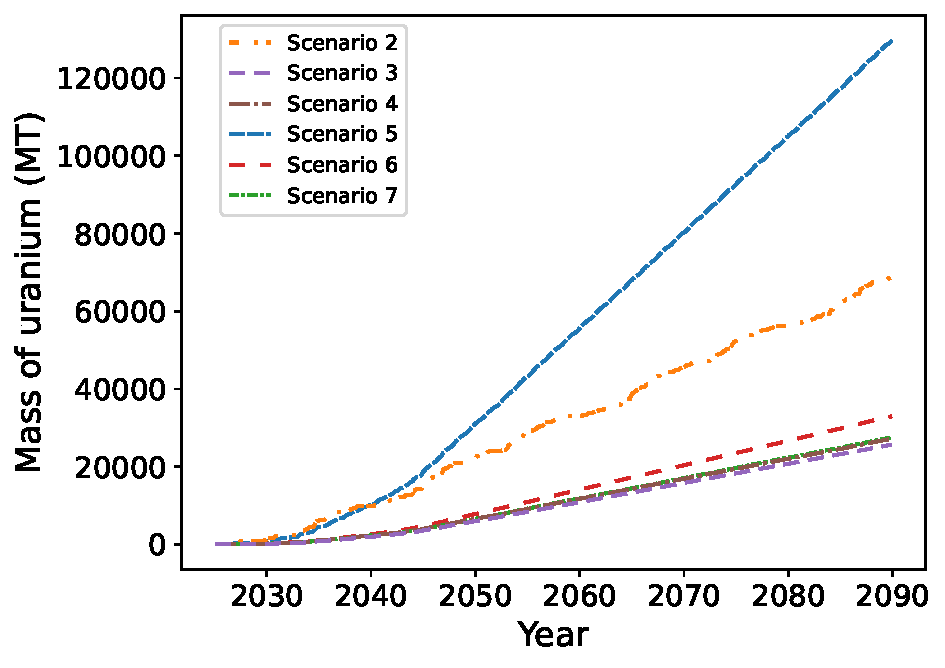
\includegraphics[width=\textwidth]{nogrowth_uranium_cumulative.pdf}
        \caption{Cumulative mass sent to advanced reactors between 2025-2090.}
        \label{fig:nogrowth_uranium_cumulative}
    \end{subfigure}
       \caption{Mass of enriched uranium required by reactors
        in Scenarios 2-7.}
       \label{fig:nogrowth_uranium}
\end{figure}

\begin{table}[h!]
    \centering 
    \caption{Metrics for enriched uranium sent to advanced 
    reactors between 2025-2090 in Scenarios 2-7.}
    \label{tab:nogrowth_uranium}
    \begin{tabular}{c c c c c}
        \hline
        Scenario & Average (MT/month) & \gls{HALEU} Average 
        (MT/month) & Maximum (MT)& Cumulative (MT)\\\hline
        2 & 88.16 & 88.16 & 1,139 & 68,674\\
        3 & 32.96 & 32.96 & 90.50 & 25,676\\
        4 & 34.94 & 34.94 & 95.41 & 27,222\\
        5 & 166.5 & 3.198 & 568.1 & 129,704\\
        6 & 42.36 & 30.69 & 106.2 & 33,000\\
        7 & 35.39 & 34.50 & 95.41 & 27,572\\
        \hline
    \end{tabular}
\end{table}

The uranium usage of each advanced reactor dictates the uranium requirements 
of each scenario. The \gls{MMR} has the smallest specific power (thermal 
power per unit mass) for a single core mass and the Xe-100 has the largest 
specific power. This metric means that to meet the same thermal power 
output, the Xe-100 will require the least uranium mass, followed by the 
VOYGR then the \gls{MMR}. However, this does not include any fuel needed for 
refueling. The \gls{MMR} does not need any uranium for refueling, but the 
Xe-100 and VOYGR do. The Xe-100 requires a smaller mass for each refueling 
than the VOYGR and a smaller mass over the same amount of time. Therefore, 
the VOYGR requires the most mass over a given period of time to produce 
a certain amount of power (accounting for refueling schemes and power  
output). This larger mass requirement of the VOYGR leads to the 
masses required by Scenario 5, which primarily deploys VOYGRs, and
contributes to the larger mass of enriched uranium in Scenario 6, compared 
with Scenario 7.

Comparing the \gls{MMR} and Xe-100, the Xe-100 requires less uranium than 
the \gls{MMR},
and the least of all three advanced reactors, over a given period of time 
to produce a given amount of power. The reduced uranium mass results 
from the high burnup of the Xe-100, so the reactor gets more energy out of 
each mass of fuel and has a larger power output. This reduced uranium mass 
required by the Xe-100 leads to Scenario 3 requiring the least 
enriched uranium by deploying only Xe-100s. Scenarios 4, 6, and 7 require similar 
masses of uranium because Xe-100s constitute a majority of the advanced 
reactors deployed and largely control the uranium required. 

Scenario 2 requires the largest average mass of \gls{HALEU}, because 
of the large number of \glspl{MMR} deployed in this scenario. Scenario 
5 requires the smallest average mass of \gls{HALEU}, despite requiring the 
largest average mass of enriched uranium, because most of the 
reactors in Scenario 5 are VOYGRs which do not require \gls{HALEU}. 
All of the other scenarios (Scenarios 3, 4, 6, and 7) require similar 
average masses of uranium and \gls{HALEU} because they deploy similar 
numbers for each type of reactor. 

Scenarios 2 and 5 require the largest mass of enriched uranium at a single 
time step. For Scenario 2, the large difference between the average and 
maximum amount of uranium is because of the refueling scheme for the 
\gls{MMR}. The \gls{MMR} only requires fuel when it is first being 
commissioned, therefore they do not require uranium at time periods in 
which
new reactors are not deployed. Additionally, the \gls{MMR} refueling scheme 
causes the variation in the monthly requirements and annual averages of 
enriched uranium masses observed in Figure \ref{fig:nogrowth_uranium}. 
The large difference between the 
monthly average and the maximum presents challenges in designing enrichment 
and fuel fabrication facilities 
to meet the demand. Designing such facilities would have to consider the 
material demands and lead times while also limiting the amount of stockpiled enriched 
uranium at each the facility, as idle stockpiles of enriched uranium 
poses a proliferation risk. 

Finally, Scenario 5 requires the largest cumulative mass of enriched uranium 
for the no growth scenarios, because the VOYGR requires more uranium than 
the other two reactors and this scenario primarily deploys VOYGRs. Scenario 3 
requires the smallest cumulative 
mass of enriched uranium, because the Xe-100 requires the smallest mass of 
uranium of the advanced reactors. The advanced reactors 
in all of these scenarios require a smaller cumulative mass of fuel than 
the \glspl{LWR}. Additionally, deploying the VOYGR in tandem with the other 
advanced reactors results in an increase in the cumulative mass 
of enriched uranium needed (e.g., Scenario 3 compared with Scenario 6). This
trend suggests that deploying VOYGRs increases the enriched uranium needs 
of the fuel cycle, even if it decreases the amount of \gls{HALEU} needed. 

The cumulative \gls{HALEU} need by 2050 for each scenario (Table 
\ref{tab:nogrowth_haleu}) is similar to the mass reported by 
Dixon et al. \cite{dixon_estimated_2022}, 5350 MTU, with the exception 
of Scenarios 2 and 5. Scenario 2 requires a greater cumulative mass of 
\gls{HALEU} because of the large number of \glspl{MMR} deployed. Scenario 
5 requires a much lower mass of \gls{HALEU} because this scenario primarily 
deploys VOYGRs. 

\begin{table}[h!]
    \centering 
    \caption{Cumulative HALEU needs by 2050 for Scenarios 2-7.}
    \label{tab:nogrowth_haleu}
    \begin{tabular}{c c}
        \hline 
        Scenario & Cumulative mass (MT) \\
        \hline
        2 & 22,223\\
        3 & 5,936 \\
        4 & 6,529 \\
        5 & 798 \\
        6 & 5,509 \\
        7 & 6,430 \\
        \hline        
    \end{tabular}
\end{table}

\subsubsection{Feed uranium}
For the mass of feed uranium, Scenario 2 requires the largest average mass 
to supply the advanced reactors (Figure \ref{fig:nogrowth_feed}, Table 
\ref{tab:nogrowth_feed}). Scenario 2 requires the most feed uranium 
because it requires more enriched uranium than most 
of the other no growth scenarios and it requires the highest product 
assay. As shown by Eq. \ref{eq:enrichment_assasys}, as the product assay 
increases, the mass of feed uranium increases, assuming all other 
variables are constant. Therefore, the combination of an increased product 
mass and an increased product assay results in a large increase in the feed 
mass required. Scenario 5 requires the next largest average 
mass of feed uranium. This scenario requires less feed uranium than Scenario 2 
because 
most of the product uranium for this scenario is for the VOYGRs, which 
require a lower enrichment assay than the \glspl{MMR}. Based on Eq. 
\ref{eq:enrichment_assasys}, a lower product assay results in 
a lower mass of feed material required. The decrease in the product 
assay overpowers the increase in feed required by the increased product mass. 
Scenario 5 still requires more feed 
material than the other scenarios because the average product mass required 
is much larger than the other scenarios, which offsets some of the decrease 
in feed material from the decrease in the product assay. 

\begin{figure}[h!]
    \centering
    \begin{subfigure}[b]{0.45\textwidth}
        \centering
        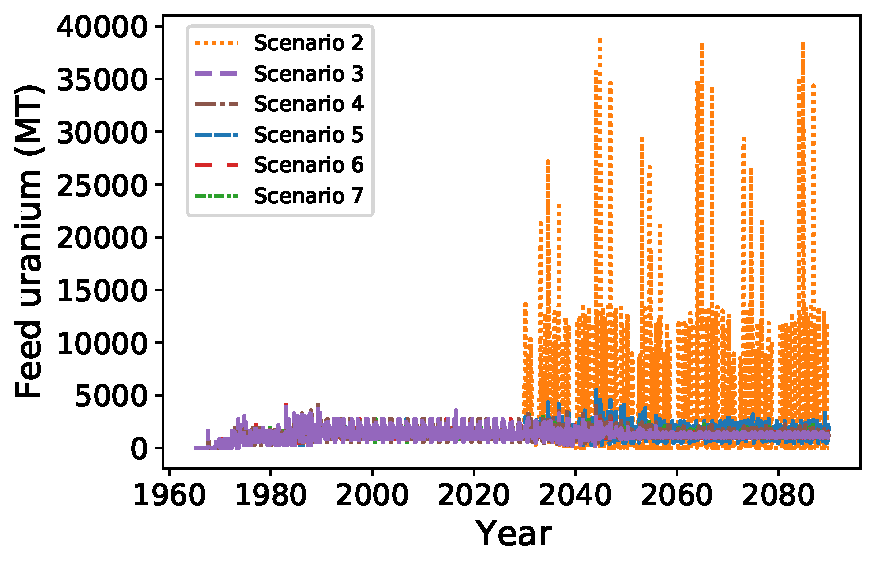
\includegraphics[width=\textwidth]{nogrowth_feed.pdf}
        \caption{Monthly mass to support all reactors between 1965-2090.}
        \label{fig:nogrowth_all_feed}
    \end{subfigure}
    \hfill
    \begin{subfigure}[b]{0.45\textwidth}
        \centering
        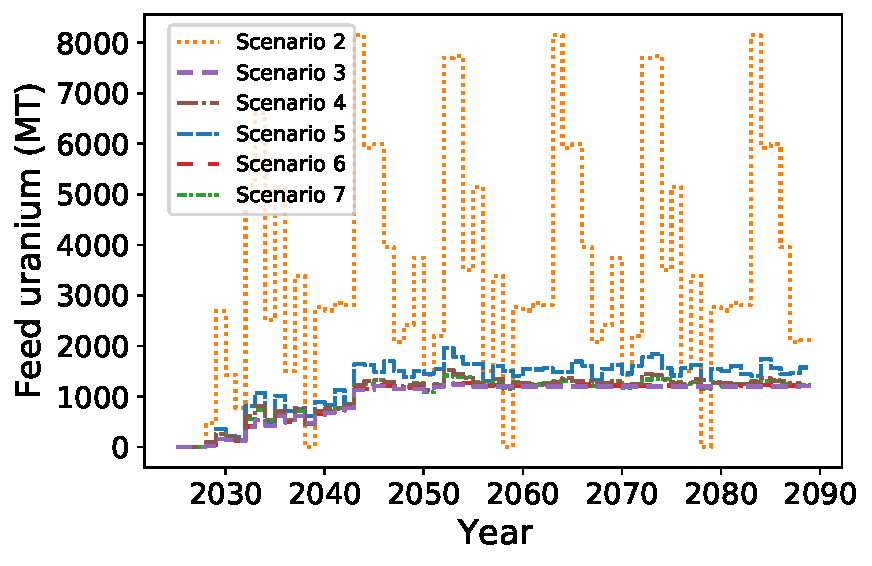
\includegraphics[width=\textwidth]{nogrowth_AR_feed.pdf}
        \caption{Annual average mass to support
        advanced reactors between 2025-2090.}
        \label{fig:nogrowth_AR_feed}
    \end{subfigure}
    \begin{subfigure}[b]{0.45\textwidth}
        \centering
        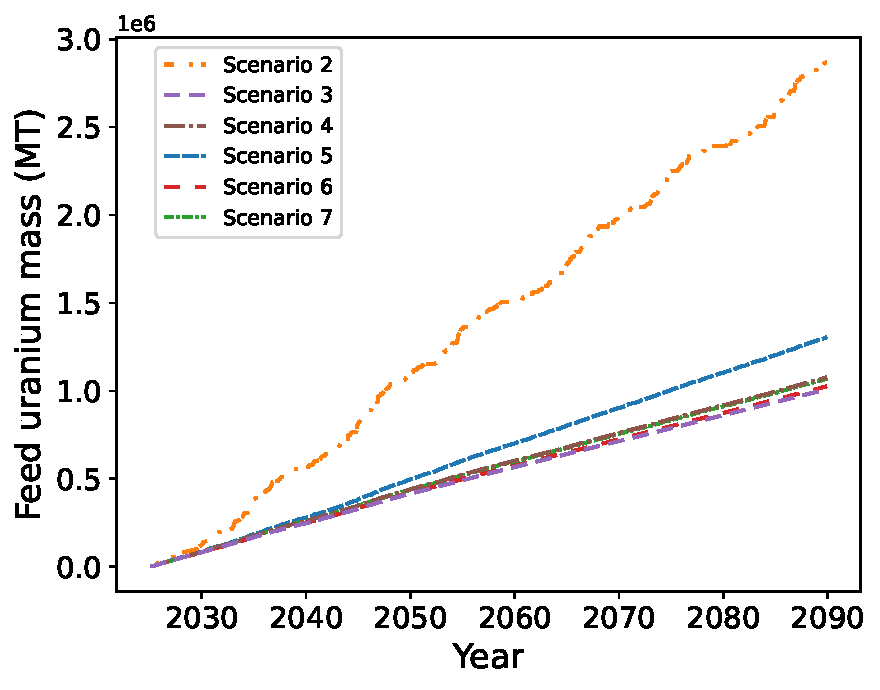
\includegraphics[width=\textwidth]{nogrowth_feed_cumulative.pdf}
        \caption{Cumulative mass to support advanced reactors between 2025-2090.}
        \label{fig:nogrowth_feed_cumulative}
    \end{subfigure}
       \caption{Mass of feed uranium required to produce enriched uranium
        in Scenarios 2-7.}
       \label{fig:nogrowth_feed}
\end{figure}

\begin{table}[h!]
    \centering 
    \caption{Metrics for feed uranium required by advanced reactors 
    between 2025-2090 in Scenarios 2-7.}
    \label{tab:nogrowth_feed}
    \begin{tabular}{c c c c c}
        \hline
        Scenario & Average (MT/month) & \gls{HALEU} Average 
        (MT/month) & Maximum (MT) & Cumulative (MT)\\\hline
        2 & 3,372 & 3,372 & 43,612 & 2,627,374\\
        3 & 986.9 & 986.9 & 2,710 & 768,793\\
        4 & 1,073 & 1,073 & 2,912 & 835,887\\
        5 & 1,365 & 122.4 & 4,896 & 1,063,737\\
        6 & 1,008 & 918.9 & 2,768 & 785,020\\
        7 & 1,063 & 1,056 & 2,912 & 828,036\\
        \hline
    \end{tabular}
\end{table}

When comparing the feed material to create \gls{HALEU} in each scenario, 
Scenario 2 requires the most feed material because this scenario 
requires the largest average mass of \gls{HALEU} and \gls{HALEU} at the 
highest product assay. Scenario 5 requires the least feed material for 
\gls{HALEU} because the majority of 
the reactors in this scenario are VOYGRs.
Additionally, fueling the Xe-100 requires less feed uranium than fueling 
the \gls{MMR} because the Xe-100 requires a lower product assay and a 
smaller product mass per core. 
Scenarios 3, 4, and 7 require similar feed uranium masses (about 1,000 
MTU/month). Deploying VOYGRs alongside the other advanced 
reactors (e.g., between Scenarios 3 and 6) decreases the average 
mass of feed uranium to create \gls{HALEU}. Deploying VOYGRs decreases the 
average of all feed uranium if \glspl{MMR} are also deployed, because the 
decrease in product assay between these reactors offsets the increase in 
total product mass when calculating the feed mass. 

The maximum feed uranium required by each scenario poses some 
challenge in facility design. The maximum feed uranium required varies 
between 2.7-12.9 times larger than the average feed material, which means 
facilities that produce feed uranium will likely need to be designed with a 
larger capacity than the average feed uranium required to meet the peaks. 
The cumulative mass of feed uranium required by each scenario ranges between 
737,000-978,000 MT for every scenario except Scenario 2. 
Scenario 2 requires over 2.64 million MT, which is more feed uranium 
than what is required by the \glspl{LWR}. The \gls{EIA} reports 
about 176,000 MT of U$_3$O$_8$ reserves in the US available at up to 
\$100/pound at the end of 2019 \cite{us_energy_information_administration_2020_2021}, 
or about 
149,000 MT of uranium, which is smaller than the cumulative needs for 
all of these scenarios. Therefore, the US would have to consider either uranium 
from international sources or uranium reserves at increased 
prices to meet the cumulative demand of feed 
uranium for each of these scenarios.

\subsection{1\% growth scenarios}
\subsubsection{Enriched uranium}
The trends observed in the 1\% growth scenarios match the trends 
observed with the no growth scenarios that deploy the same reactor 
types (i.e., Scenarios 2 and 8), as shown in 
Figure \ref{fig:1percent_uranium} and Table \ref{tab:1percent_uranium}. 
Scenario 11 requires the largest average mass of enriched uranium, and Scenario
8 requires the next largest average. Scenario 8 requires the largest 
average mass of \gls{HALEU}, while Scenario 11 requires the least. Scenario 
8 requires an average of 141.8 MT of \gls{HALEU} per month, Scenario 
9 requires the 
smallest monthly average of enriched uranium, because this scenario 
deploys the least number of reactors, and the Xe-100 requires the smallest 
mass of fuel in the core. 

\begin{figure}[h!]
    \centering
    \begin{subfigure}[b]{0.45\textwidth}
        \centering
        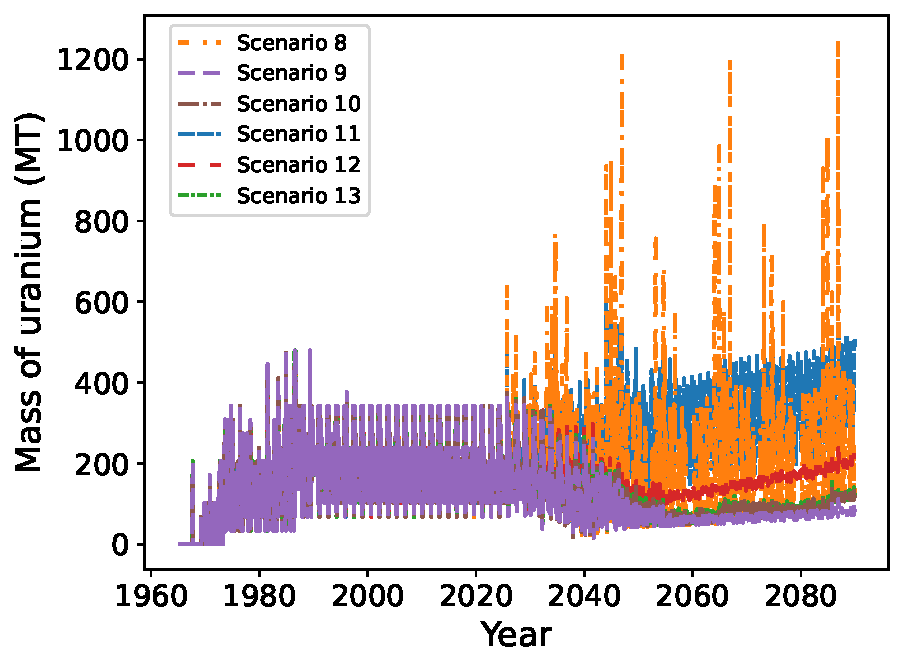
\includegraphics[width=\textwidth]{1percent_uranium.pdf}
        \caption{Monthly mass sent to all reactors between 1965-2090.}
        \label{fig:1percent_all_uranium}
    \end{subfigure}
    \hfill
    \begin{subfigure}[b]{0.45\textwidth}
        \centering
        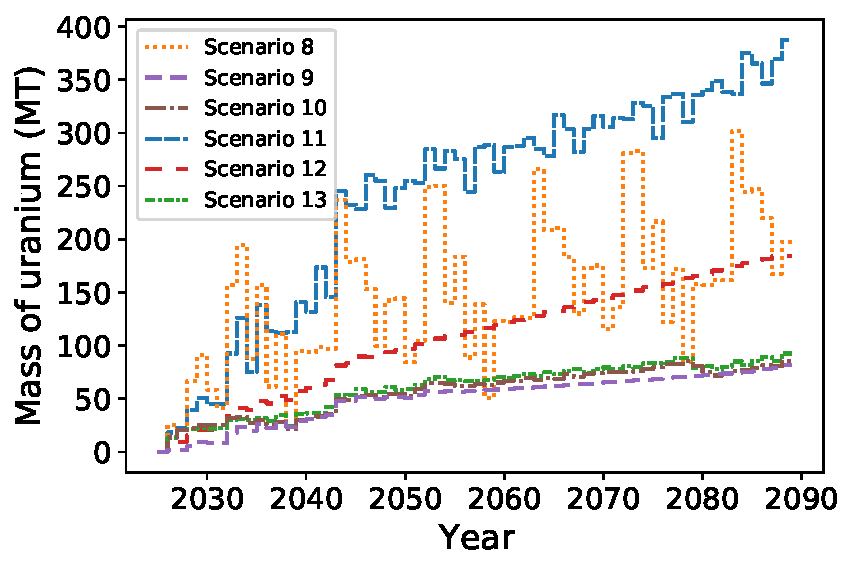
\includegraphics[width=\textwidth]{1percent_AR_uranium.pdf}
        \caption{Annual average mass sent to 
        advanced reactors between 2025-2090.}
        \label{fig:1percent_AR_uranium}
    \end{subfigure}
    \begin{subfigure}[b]{0.45\textwidth}
        \centering
        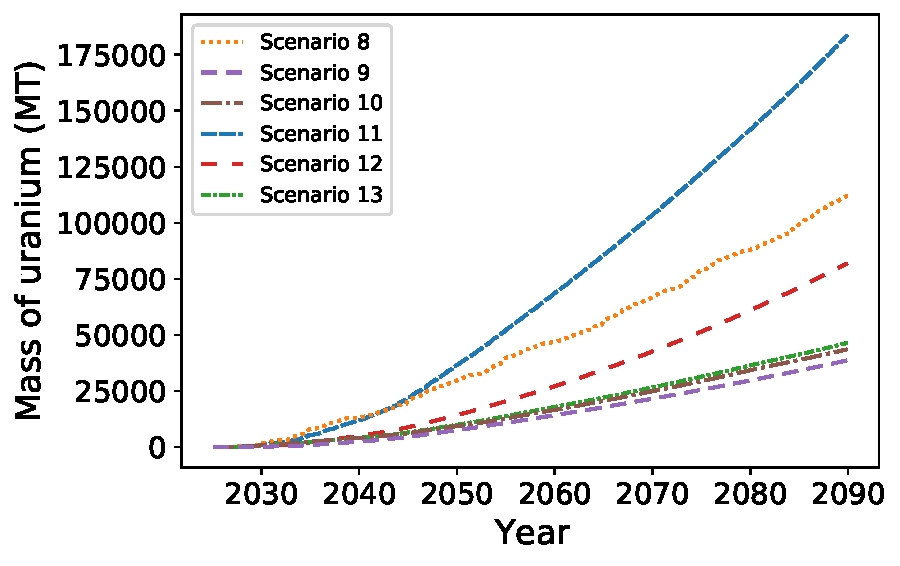
\includegraphics[width=\textwidth]{1percent_uranium_cumulative.pdf}
        \caption{Cumulative mass sent to advanced reactors 
        between 2025-2090.}
        \label{fig:1percent_uranium_cumulative}
    \end{subfigure}
       \caption{Mass of enriched uranium required by reactors
        in Scenarios 8-13.}
       \label{fig:1percent_uranium}
\end{figure}

\begin{table}[h!]
    \centering 
    \caption{Metrics for enriched uranium required by advanced reactors 
    between 2025-2090 in Scenarios 8-13.}
    \label{tab:1percent_uranium}
    \begin{tabular}{c c c c c}
        \hline
        Scenario & Average (MT/month) & \gls{HALEU} Average  
        (MT/month) & Maximum (MT) & Cumulative (MT)\\\hline
        8 & 141.8 & 141.8 & 1,246 & 110,486\\
        9 & 51.47 & 51.47 & 112.50 & 40,097\\
        10 & 65.01 & 65.01 & 145.6 & 50,643\\
        11 & 251.1 & 18.93 & 606.2 & 195,645\\
        12 & 114.1 & 36.42 & 237.7 & 88,910\\
        13 & 68.19 & 61.98 & 157.8 & 53,118\\
        \hline
    \end{tabular}
\end{table}

Scenario 12 requires a larger monthly average mass of enriched uranium 
than Scenarios 9, 10, and 13. The no growth scenarios exhibit this result
as well, but it is more pronounced in the 1\% growth scenarios (comparing 
Figures \ref{fig:nogrowth_uranium} and \ref{fig:1percent_uranium}). 
The more pronounced result in the 1\% growth scenarios is a result of the difference 
in energy demand and the deployment scheme. Scenarios 6 and 12 deploy the 
Xe-100 and the VOYGR. The increase in energy demand in Scenario 12 results 
in more VOYGRs deployed relative to the number of Xe-100s deployed. 
The VOYGR meeting more of the energy demand in Scenario 12 and the VOYGR 
requiring more enriched uranium than the Xe-100 lead to more 
enriched uranium needed for Scenario 12, relative to other scenarios 
that deploy Xe-100s.

The maximum mass of enriched uranium required in each scenario ranges 
between 2.2-8.8 times the average monthly mass, which is a smaller ratio 
than for the no growth scenarios. The increase between 
the average and the maximum is smaller for the 1\% growth scenarios because
the averages increase more than the maximums for the scenarios deploying the 
same reactors (e.g., between Scenarios 2 and 8). The cumulative mass 
of enriched uranium required has a similar pattern to the average mass;
Scenario 11 requires the most mass, followed by Scenario 8. Scenario 
9 requires the smallest cumulative mass. 
The advanced reactors in Scenario 11 require more enriched uranium 
than the \glspl{LWR}, but the other scenarios require less than the 
\glspl{LWR}. 

 

\subsubsection{Feed uranium}
The trends of the mass of feed uranium required by Scenarios 8-13 
(Figure \ref{fig:1percent_feed},
Table \ref{tab:1percent_feed}) are consistent with trends of the feed 
requirements of the no growth scenarios. Scenario 8 requires the 
most feed uranium based on any of the metrics in Table 
\ref{tab:1percent_feed}, because of the larger number of 
reactors deployed than the other scenarios and all of the reactors deployed 
require \gls{HALEU}. The larger product assay of \gls{HALEU}, compared with 
the product assay for \glspl{LWR} or VOYGRs, means that more 
feed uranium is needed to produce the same product mass (Eq. 
\ref{eq:enrichment_assasys}). Scenario 11 requires the next largest amount 
of feed uranium, with most of the feed uranium used to produce enriched 
uranium for the VOYGRs. The other scenarios require similar monthly 
averages of feed uranium, with Scenario 9 requiring the least amount of 
feed uranium. The similarity in feed uranium required by Scenarios 9, 10, 12, 
and 13 is a result of the Xe-100 and VOYGR requiring similar feed uranium masses 
and the deployment scheme primarily deploying the Xe-100 and VOYGR in each of 
these scenarios. Scenarios 10, 11, and 13 require more feed 
uranium than Scenarios 9 and 12, because of the deployment of \glspl{MMR} 
in Scenarios 10, 11, and 13 and the \gls{MMR} requiring more feed uranium than 
the Xe-100 and VOYGR. To produce \gls{HALEU}, Scenario 8 requires the most 
feed uranium and Scenario 11 requires the least.  

\begin{figure}[h!]
    \centering
    \begin{subfigure}[b]{0.45\textwidth}
        \centering
        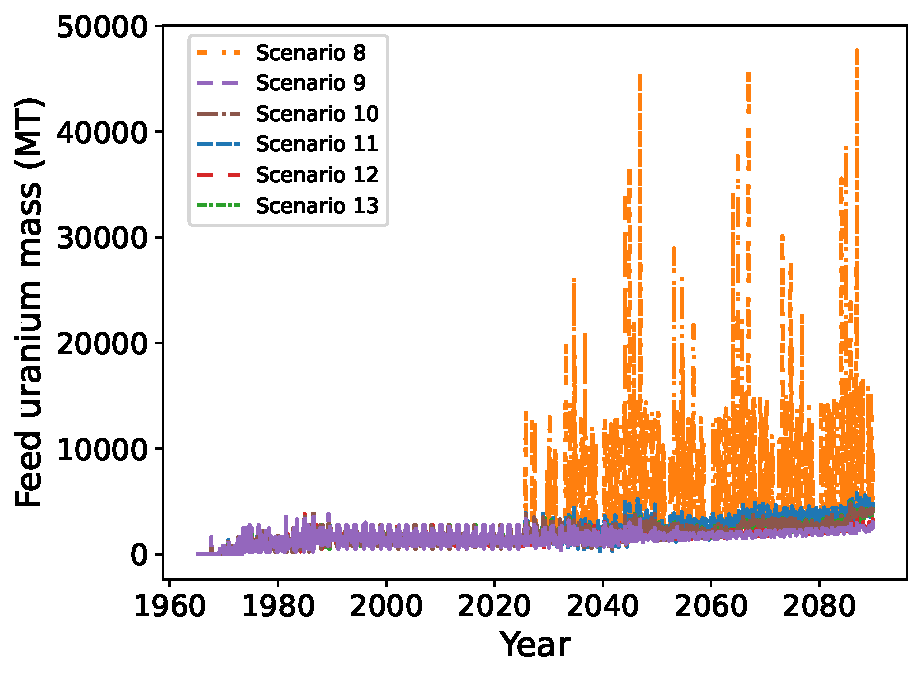
\includegraphics[width=\textwidth]{1percent_feed.pdf}
        \caption{Monthly mass to support
        all reactors between 1965-2090.}
        \label{fig:1percent_all_feed}
    \end{subfigure}
    \hfill
    \begin{subfigure}[b]{0.45\textwidth}
        \centering
        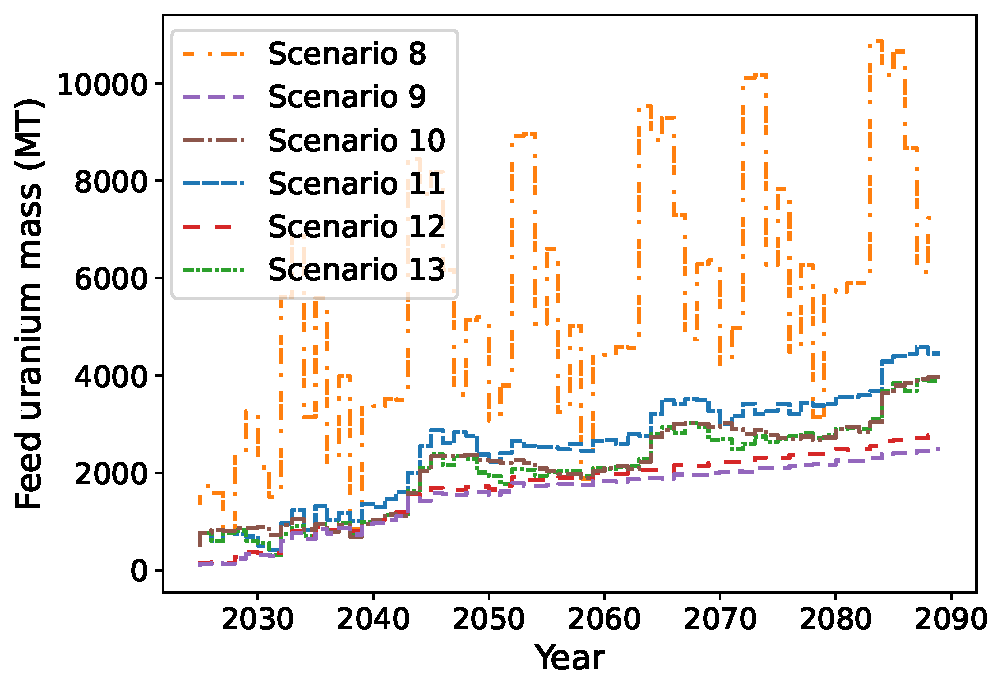
\includegraphics[width=\textwidth]{1percent_AR_feed.pdf}
        \caption{Annual average mass to support advanced reactors between 2025-2090.}
        \label{fig:1percent_AR_feed}
    \end{subfigure}
    \begin{subfigure}[b]{0.45\textwidth}
        \centering
        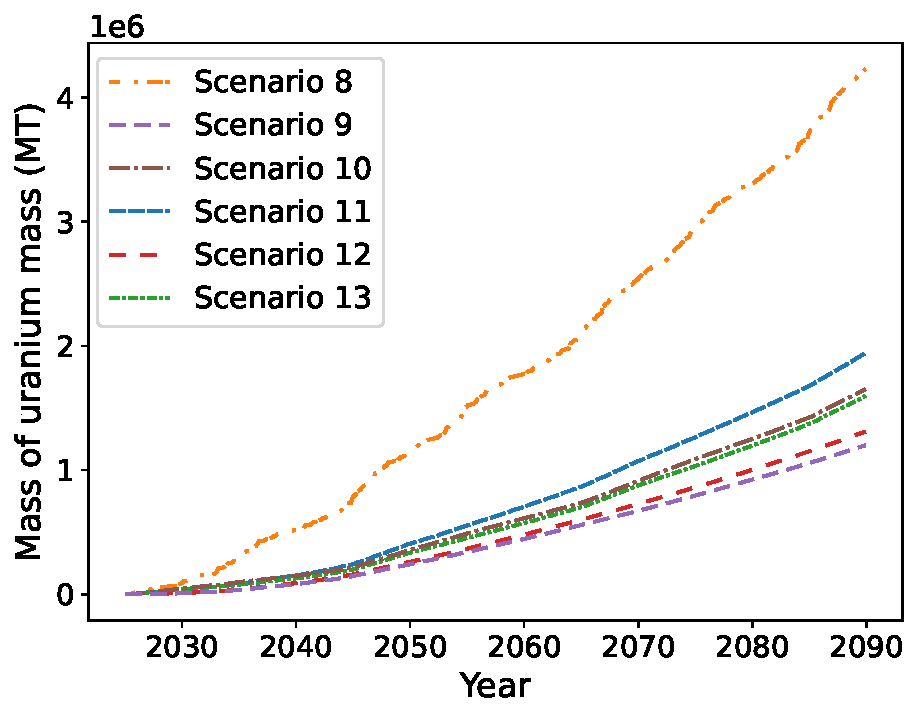
\includegraphics[width=\textwidth]{1percent_feed_cumulative.pdf}
        \caption{Cumulative mass to support 
        advanced reactors between 2025-2090.}
        \label{fig:1percent_feed_cumulative}
    \end{subfigure}
       \caption{Mass of feed uranium required to produce enriched uranium
       at each time step in Scenarios 8-13.}
       \label{fig:1percent_feed}
\end{figure}

\begin{table}[h!]
    \centering 
    \caption{Metrics for feed uranium required by advanced reactors 
    between 2025-2090 in Scenarios 8-13.}
    \label{tab:1percent_feed}
    \begin{tabular}{c c c c c}
        \hline
        Scenario & Average (MT/month) & \gls{HALEU} Average  
        (MT/month) & Maximum (MT) & Cumulative (MT)\\\hline
        8 & 5,426 & 5,426 & 47,689 & 4,226,992\\
        9 & 1,541 & 1,541 & 3,368 & 1,200,546\\
        10 & 2,119 & 2,119 & 4,813 & 1,651,029\\
        11 & 2,491 & 724.2 & 5,801 & 1,941,265\\
        12 & 1,682 & 1,090 & 3,679 & 1,310,418\\
        13 & 2,050 & 2,003 & 4,987 & 1,597,312\\
        \hline
    \end{tabular}
\end{table}

The maximum feed uranium required varies between 2.2-8.8 times the monthly 
average of all feed uranium, which is similar to the ratios of the 
maximum and average masses required for enriched uranium. Scenario 8 
requires the largest maximum peak of 
feed uranium, corresponding to the deployment of 936 \glspl{MMR}. Because 
of 
the large number of reactors and the large mass of feed uranium required 
in Scenario 8, the cumulative mass of feed uranium quickly diverges from 
the cumulative mass of the other scenarios after the transition start time. 

\section{SWU capacity}
This section reports the results of the \gls{SWU} capacity 
required to support the advanced reactors in the transition 
scenarios. The \gls{SWU} requirements were calculated using 
Eq. \ref{eq:enrichment},  
the mass of enriched uranium, the feed uranium required, 
and the assay of each material stream (feed, tails, and product)
in each scenario. This metric relates to the facility capacity 
and design required to enrich natural uranium and produce 
enriched uranium for each scenario. Understanding this metric, 
and specifically how much \gls{SWU} capacity is required to 
produce \gls{HALEU} is vital to developing infrastructure to 
produce \gls{HALEU}. Unless specified as \gls{SWU} capacity to 
produce \gls{HALEU}, the reported \gls{SWU} capacities are 
required to produce any enriched uranium less than 20\% 
$^{235}$U. 

\subsection{No growth scenarios} \label{sec:nogrowth_swu}
The \gls{SWU} capacity required to produce the enriched uranium for 
the no growth scenarios follows a similar pattern as 
the feed uranium required by each scenario (Figure \ref{fig:nogrowth_swu}, 
Table \ref{tab:nogrowth_swu}). Scenario 2 requires the largest average 
monthly capacity, average monthly capacity to produce \gls{HALEU}, and maximum 
capacity needed. Scenario 3 requires the smallest average for the total 
\gls{SWU} capacity, 
and Scenario 5 requires the smallest average 
\gls{SWU} capacity to produce \gls{HALEU}. Scenario 3 requires the least 
\gls{SWU} capacity because it only deploys Xe-100s, which require the 
smallest \gls{SWU} capacity to produce a core-load of fuel. Scenario 
6 requires a very similar \gls{SWU} capacity to support all of the 
advanced reactors because the Xe-100 and VOYGR (which are both deployed 
in Scenario 6) require similar \gls{SWU} capacity. The increased 
product assay required by the Xe-100, compared with the VOYGR, evens 
out with the decrease in product mass to result in similar \gls{SWU} 
requirements to produce enriched uranium for these two reactors. 
Scenario 2 requires a larger average \gls{SWU} capacity 
than the \glspl{LWR} before 2025 because of the greater product 
assay required by the \gls{MMR}. 

\begin{figure}[h!]
    \centering
    \begin{subfigure}[b]{0.45\textwidth}
        \centering
        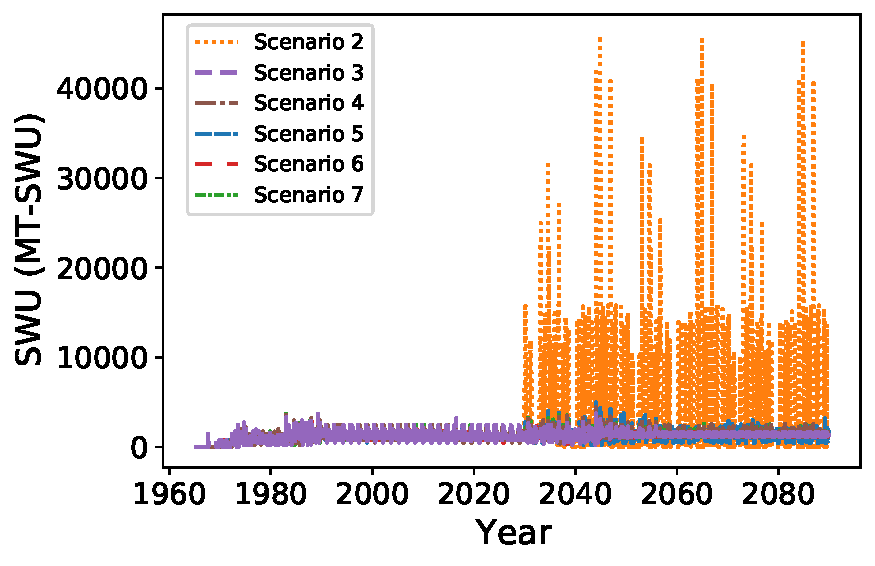
\includegraphics[width=\textwidth]{nogrowth_SWU.pdf}
        \caption{Monthly \gls{SWU} capacity to support all reactors between 1965-2090.}
        \label{fig:nogrowth_all_SWU}
    \end{subfigure}
    \hfill
    \begin{subfigure}[b]{0.45\textwidth}
        \centering
        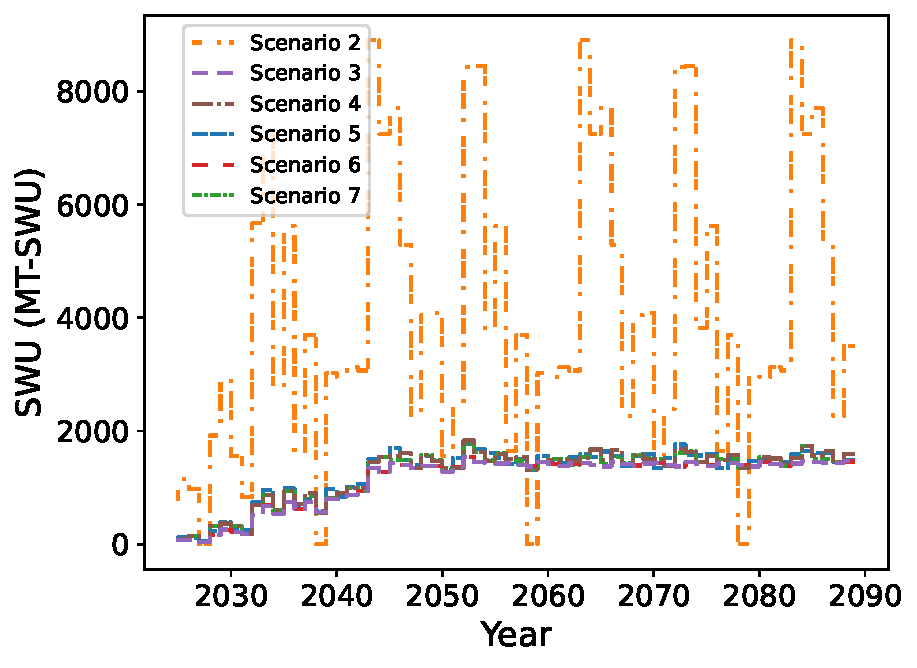
\includegraphics[width=\textwidth]{nogrowth_AR_SWU.pdf}
        \caption{Annual average \gls{SWU} capacity to support advanced reactors between 2025-2090.}
        \label{fig:nogrowth_AR_SWU}
    \end{subfigure}
       \caption{\gls{SWU} capacity required to produce enriched uranium 
       for reactors in Scenarios 2-7.}
       \label{fig:nogrowth_swu}
\end{figure}

\begin{table}[h!]
    \centering 
    \caption{Metrics for \gls{SWU} capacity to enrich uranium for 
    advanced reactors between 2025-2090 in Scenarios 2-7.}
    \label{tab:nogrowth_swu}
    \begin{tabular}{c c c c}
        \hline
        Scenario & Average  (MT-SWU/month) & Average
        for \gls{HALEU} (MT-SWU/month) & Maximum (MT-SWU)\\\hline
        2 & 3,978 & 3,978 & 51,433 \\
        3 & 1,136 & 1,136 & 3,119\\
        4 & 1,238 & 1,238 & 3,360\\
        5 & 1,246 & 144.3 & 4,550 \\
        6 & 1,137 & 1,058 & 3,149\\
        7 & 1,224 & 1,218 & 3,360\\
        \hline
    \end{tabular}
\end{table}

The \gls{SWU} capacity required to produce \gls{HALEU} decreases when 
deploying the VOYGR along with the other reactors, with the exception 
of deploying the VOYGR with both \gls{HALEU}-fueled reactors, as noted 
with the feed uranium requirements. 
Scenario 5 requires the least \gls{SWU} capacity to produce 
\gls{HALEU} because most of the enriched uranium in this 
scenario is for VOYGRs which don't require \gls{HALEU}. However, this 
scenario requires a similar average \gls{SWU} capacity as most of the other 
scenarios because of the off-setting effect of the increase in product mass 
and decrease in product assay between the Xe-100 and VOYGR. 

The maximum \gls{SWU} capacity required to meet enriched uranium demand 
varies between 2.7-12.9 times the monthly average for all \gls{SWU}. 
The magnitude differences between the average and the maximum pose potential 
problems for facility design and nonproliferation safeguards. Facilities 
will likely need to be built at a capacity greater than the average 
monthly requirement in order to produce enough enriched uranium to meet 
the peak demands. However, such a design may result in idle enrichment 
capacity during time periods in which the additional capacity is 
not needed to meet peaks, which poses a proliferation risk. Additionally, 
the \gls{SWU} requirements reported here do not account for different 
centrifuge cascade designs required to produce enriched uranium for 
each advanced reactor. Cascade designs will differ based on 
the amount of material needed (more material means more centrifuges in 
parallel) and the product assay (higher product assay means more stages), 
and understanding how to establish the cascades to support these transition 
scenarios would require additional exploration. 

\subsection{1\% growth scenarios}
The \gls{SWU} capacity required to meet the enriched uranium demand of 
the 1\% growth scenarios 
follows similar patterns as the \gls{SWU} capacity required in the no 
growth scenarios (Figure \ref{fig:1percent_swu}, Table \ref{tab:1percent_swu}).
Scenario 8 requires the largest average \gls{SWU} 
capacity and the largest \gls{SWU} capacity to create \gls{HALEU}, Scenario 
9 requires the smallest average \gls{SWU} capacity to enrich uranium 
for all advanced reactors, and 
Scenario 11 requires the smallest average \gls{SWU} capacity 
to create \gls{HALEU}. Comparing 
the monthly average capacity and the monthly average capacity to produce \gls{HALEU} 
shows that most or all of the \gls{SWU} capacity needed is to produce 
\gls{HALEU}, except in Scenario 11. The 
maximum \gls{SWU} capacity required ranges between 2.2-8.9 times 
the average \gls{SWU} capacity required by each scenario. All of these 
scenarios require more \gls{SWU} capacity than the \glspl{LWR} before 
2025. 

\begin{figure}[h!]
    \centering
    \begin{subfigure}[b]{0.45\textwidth}
        \centering
        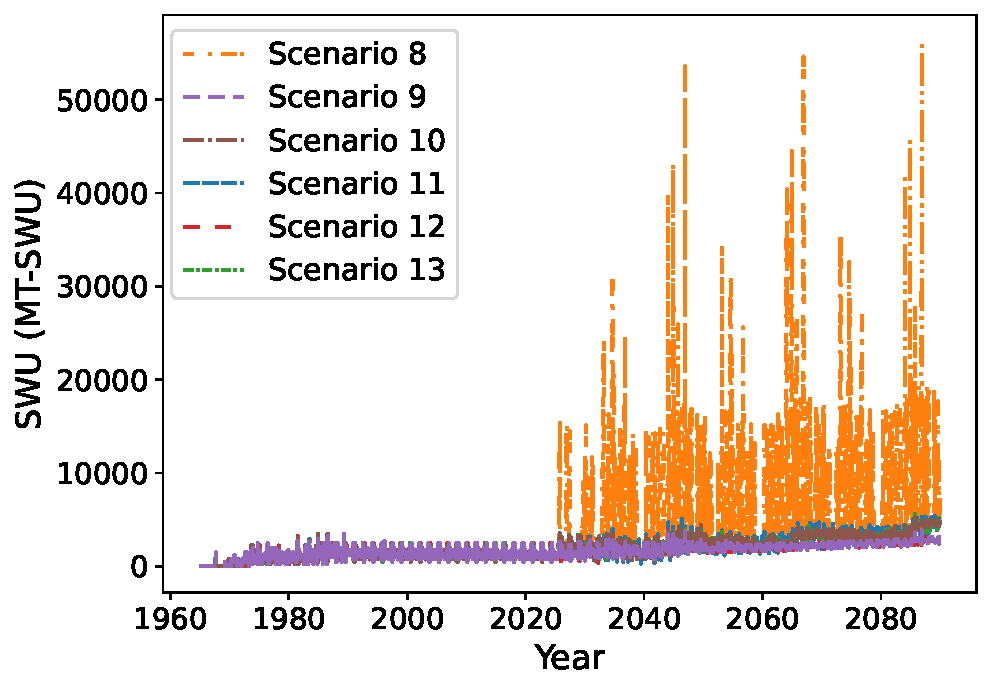
\includegraphics[width=\textwidth]{1percent_SWU.pdf}
        \caption{Monthly \gls{SWU} capacity to support all reactors between 1965-2090.}
        \label{fig:1percent_all_SWU}
    \end{subfigure}
    \hfill
    \begin{subfigure}[b]{0.45\textwidth}
        \centering
        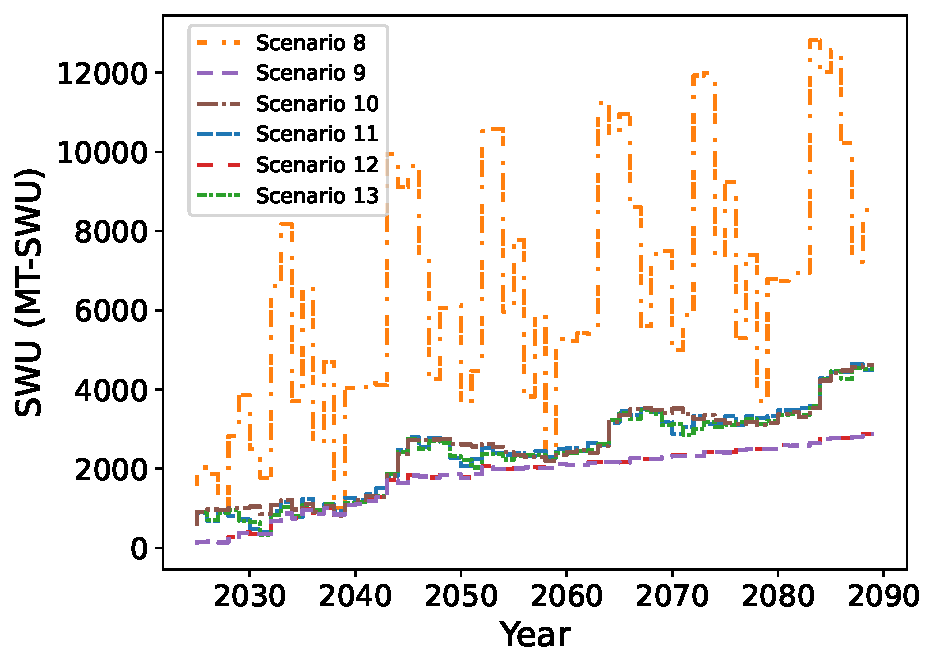
\includegraphics[width=\textwidth]{1percent_AR_SWU.pdf}
        \caption{Annual average \gls{SWU} capacity to support advanced reactors between 2025-2090.}
        \label{fig:1percent_AR_SWU}
    \end{subfigure}
       \caption{\gls{SWU} capacity required to produce enriched uranium 
       for reactors in Scenarios 8-13.}
       \label{fig:1percent_swu}
\end{figure}

\begin{table}[h!]
    \centering 
    \caption{Metrics for \gls{SWU} capacity to enrich uranium for 
    advanced reactors between 2025-2090 in Scenarios 8-13.}
    \label{tab:1percent_swu}
    \begin{tabular}{c c c c}
        \hline
        Scenario & Average (t-SWU/month) & Average  
        for \gls{HALEU} (t-SWU/month) & Maximum (t-SWU)\\\hline
        8 & 6,339 & 6,339 & 56,239 \\
        9 & 1,774 & 1,774 & 3,878\\
        10 & 2,462 & 2,462 & 5,600\\
        11 & 2,421 & 854.1 & 5,605\\
        12 & 1,780 & 1,256 & 3,926\\
        13 & 2,367 & 2,325 & 5,784\\
        \hline
    \end{tabular}
\end{table}

Scenarios 9 and 12 require very similar \gls{SWU} capacities, and 
Scenarios 10, 11, and 13 require similar \gls{SWU} capacities. 
The feed uranium requirements had the same scenario groupings. 
The difference between these scenario groupings is the deployment 
of \glspl{MMR}; Scenarios 9 and 12 do not deploy \glspl{MMR} but 
Scenarios 10, 11, and 13 deploy \glspl{MMR}. Producing enriched uranium 
for the \gls{MMR} requires more \gls{SWU} capacity than providing 
enriched uranium for the Xe-100 and VOYGR, with the Xe-100 and VOYGR 
requiring similar \gls{SWU} capacities. Combined with the inflated 
number of \glspl{MMR} deployed as a result of the deployment scheme, 
Scenarios 10, 11, and 13 require more \gls{SWU} capacity to produce 
all enriched uranium for advanced reactors by 2090 than Scenarios 9 and 12. 

\section{Spent nuclear fuel}
The final metric of interest for the once-through transition scenarios is 
the amount of \gls{SNF} that must be disposed of.
\gls{SNF} produced in a \gls{NFC} has implications on the options 
to treat and store the waste. A once-through fuel cycle will dispose of 
all of the \gls{SNF} discharged from the reactors, although 
the timing is affected by the duration in wet storage. The masses 
reported here are the masses discharged from the reactors, which 
matches the capacity needs for disposal in a dry storage system or a 
geologic repository, but not necessarily the timing of the disposal.
The masses 
presented here are the masses of all materials in the \gls{SNF}, not just 
the uranium discharged, because all materials in the \gls{SNF} must be 
disposed of. \gls{SNF} characteristics other than mass will affect repository 
and material handling needs, such as decay heat, \gls{SNF} volume, and 
criticality safety. However, reporting the mass of \gls{SNF} is common in 
fuel cycle analysis \cite{sunny_transition_2015,feng_standardized_2016,bae_standardized_2019},
which lead to the use of reporting the \gls{SNF} mass in this work. 

\subsection{No growth scenarios}
The magnitude of discharged \gls{SNF} from the advanced reactors 
(Figure \ref{fig:nogrowth_waste}) follows the same pattern as the enriched 
uranium masses, but with delayed timing. This pattern matches expectations, 
but the values are different from the masses of enriched uranium. 
This difference arises for two reasons: first, the 
\gls{SNF} masses include any carbon or oxygen in the fuel forms (UCO and 
UO$_2$), which 
are not included in the enriched uranium masses; second, the 
fuel in the reactors at the end of the simulation are not included in these 
calculations because they are not traded to the cooling pool facility.
Scenario 5 experiences the largest average mass of \gls{SNF} 
discharged but the smallest average mass of \gls{SNF} discharged from 
\gls{HALEU}-fueled reactors. 
Scenario 3 discharges the smallest average and cumulative mass of \gls{SNF}.
These trends are consistent with the mass of enriched uranium required 
in each scenario and the design characteristics of the advanced 
reactors deployed in each scenario. For example, Scenario 5 discharges the 
largest average mass of \gls{SNF} because it primarily deploys VOYGRs, which 
have a lower specific power than the Xe-100 and require more fuel per unit 
power than the Xe-100 and \gls{MMR}. 
The average mass of \gls{SNF} discharged by advanced reactors is less than 
the average discharged by \glspl{LWR} before 2025. 

\begin{figure}[h!]
    \centering
    \begin{subfigure}[b]{0.45\textwidth}
        \centering
        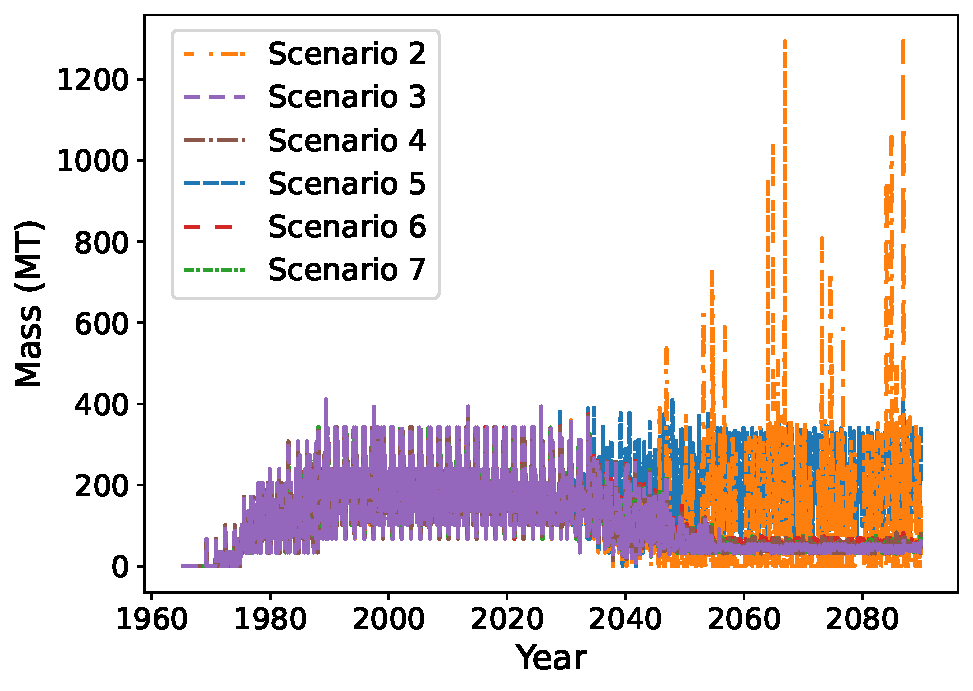
\includegraphics[width=\textwidth]{nogrowth_waste.pdf}
        \caption{Monthly mass discharged from all reactors 
        between 1965-2090.}
        \label{fig:nogrowth_all_waste}
    \end{subfigure}
    \hfill
    \begin{subfigure}[b]{0.45\textwidth}
        \centering
        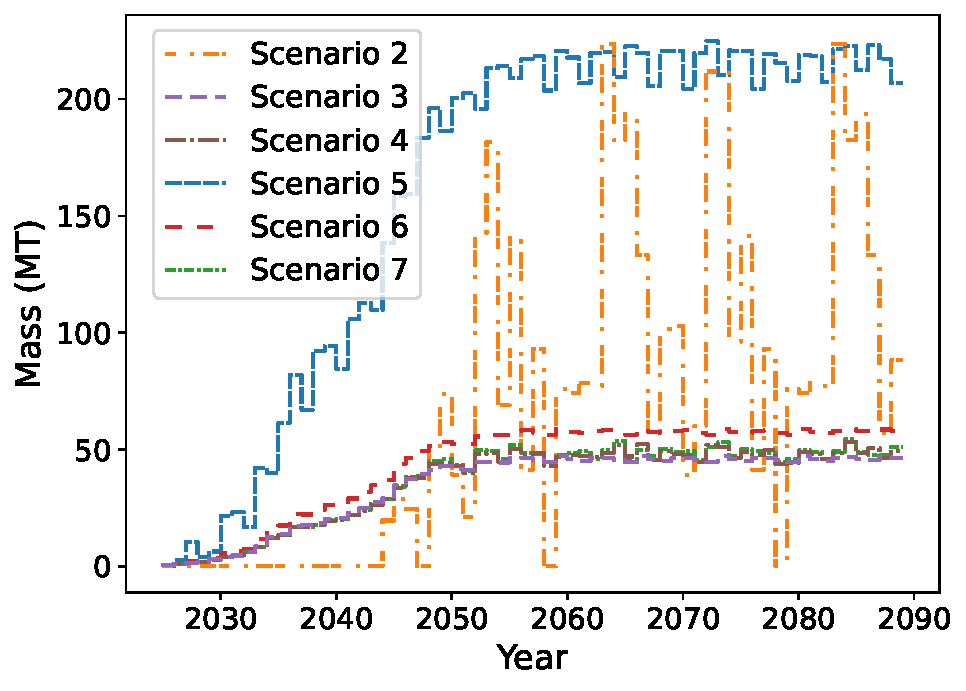
\includegraphics[width=\textwidth]{nogrowth_AR_waste.pdf}
        \caption{Annual average mass discharged from 
        advanced reactors between 2025-2090.}
        \label{fig:nogrowth_AR_waste}
    \end{subfigure}
    \begin{subfigure}[b]{0.45\textwidth}
        \centering
        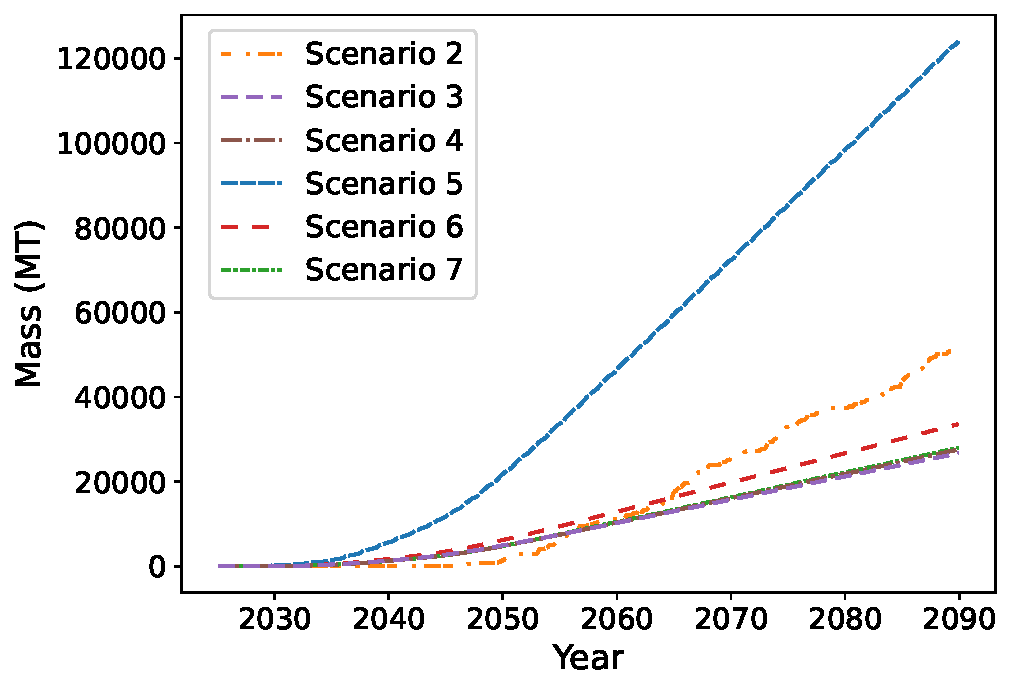
\includegraphics[width=\textwidth]{nogrowth_waste_cumulative.pdf}
        \caption{Cumulative mass discharged from advanced reactors 
        between 2025-2090.}
        \label{fig:nogrowth_waste_cumulative}
    \end{subfigure}
       \caption{Mass of fuel discharged from reactors 
       as a function of time for Scenarios 2-7. }
       \label{fig:nogrowth_waste}
\end{figure}

\begin{table}[h!]
    \centering 
    \caption{Metrics for waste discharged from advanced reactors 
    between 2025-2090 in Scenarios 2-7. The ``Average \gls{HALEU}''
    is the average mass of \gls{SNF} from \gls{HALEU}-fueled 
    reactors. }
    \label{tab:nogrowth_waste}
    \begin{tabular}{c c c c c}
        \hline
        Scenario & Average (MT/month) & Average \gls{HALEU}
        (MT/month) & Maximum (MT) & Cumulative (MT)\\\hline
        2 & 66.19 & 66.19 & 1,293 & 51,560\\
        3 & 34.29 & 34.29 & 68.13 & 26,712\\
        4 & 35.44 & 35.44 & 83.37 & 27,605\\
        5 & 159.2 & 2.395 & 406.3 & 124,016\\
        6 & 43.14 & 31.93 & 82.71 & 33,608\\
        7 & 35.95 & 35.10 & 83.37 & 28,008\\
        \hline
    \end{tabular}
\end{table}

The first \gls{SNF} discharged from advanced reactors is in June 
2030 for Scenarios 3, 4, 6, and 7, June 2031 
in Scenario 5, and 
December 2049 in Scenario 2. The differences in timing of first \gls{SNF} 
discharge from advanced reactors is a result of the refueling scheme of 
each type of reactor. Xe-100s, deployed in Scenarios 3, 4, 6, 
and 7, utilize online refueling and discharge \gls{SNF} 
every 7 months, which results in the first discharge soon after their initial 
deployment. VOYGRs, deployed in Scenarios 4, 5, 6, and 7, have an 
18-month refueling cycle, so the first \gls{SNF} discharge for these 
reactors occurs 18 months after deployment. \glspl{MMR}, deployed in 
Scenarios 2, 4, 5, and 7, do not undergo refueling, so the first \gls{SNF} 
discharge occurs 20 years after first deployment. The shortest refueling 
time of the reactors deployed in a scenario governs when 
first \gls{SNF} discharge in that scenario. Thus, the Xe-100 drives the 
first \gls{SNF} discharge in 
Scenarios 3, 4, 6, and 7, the VOYGR drives the first \gls{SNF} discharge 
in Scenario 5, and the \gls{MMR} drives the first \gls{SNF} discharge in 
Scenario 2. 

The 
advanced reactors in all of the scenarios discharge 
less \gls{SNF} than the \glspl{LWR}. The 1982 Nuclear Waste Policy Act
\cite{noauthor_nuclear_1983} requires an initial 
repository in the US to have a capacity of 70,000 MTHM. Based on this 
capacity, a geologic repository could store 
all of the waste produced from advanced reactors except for Scenario 5. 
To store all of the waste from advanced reactors in Scenario 5, either 
the repository capacity would need to be expanded or a second repository 
must be sited.

\subsection{1\% growth scenarios}
For the 1\% growth scenarios, similar patterns are observed to the 
no growth scenarios. Scenario 11 discharges  
the largest average mass of \gls{SNF} while also discharging
the smallest average mass of \gls{SNF} from \gls{HALEU}-fueled 
reactors, as shown by  
Figure \ref{fig:1percent_waste} and Table \ref{tab:1percent_waste}. 
Scenario 9 discharges the smallest average mass of \gls{SNF}. The 
first \gls{SNF} discharge 
is in November 2027 in Scenarios 9, 10, 12, and 13, in 
November 2028 in Scenario 11, and May 2047 in Scenario 8. These initial 
disposal dates are consistent with the shortest cycle time of the 
reactors deployed in each scenario (20 years in Scenario 8, 18 months in 
Scenario 11, and 6 month in Scenarios 9, 10, 12, and 13) and an 
initial deployment in May 2027. 

\begin{figure}[h!]
    \centering
    \begin{subfigure}[b]{0.45\textwidth}
        \centering
        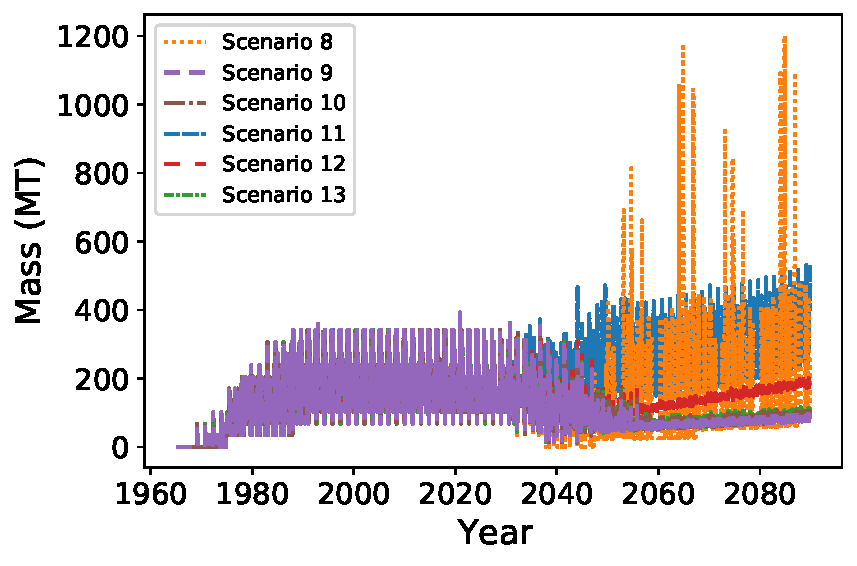
\includegraphics[width=\textwidth]{1percent_waste.pdf}
        \caption{Monthly mass discharged from all reactors between 
        1965-2090.}
        \label{fig:1percent_all_waste}
    \end{subfigure}
    \hfill
    \begin{subfigure}[b]{0.45\textwidth}
        \centering
        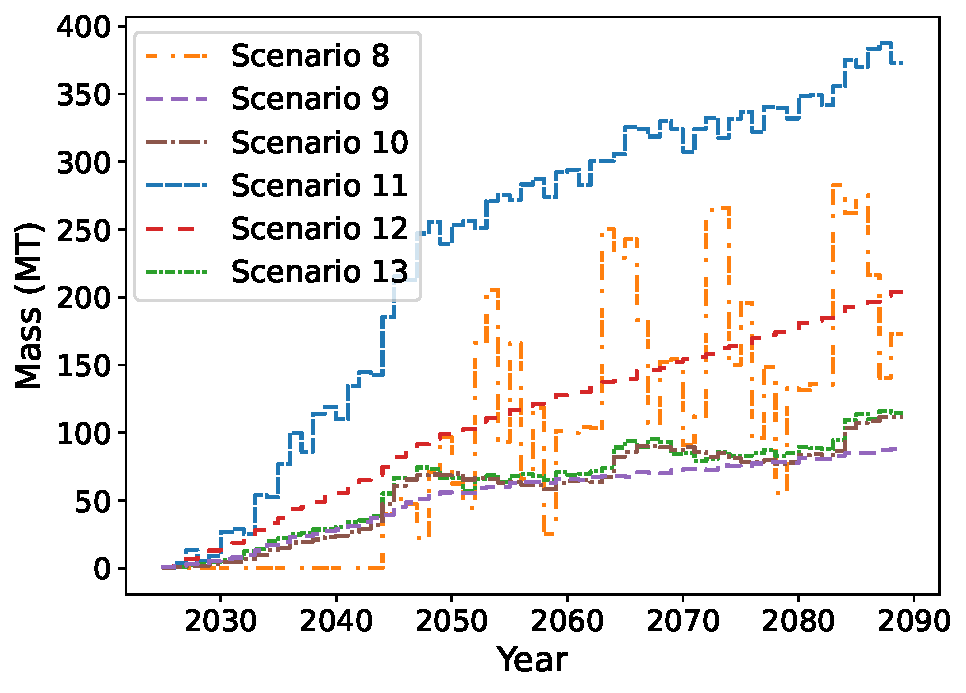
\includegraphics[width=\textwidth]{1percent_AR_waste.pdf}
        \caption{Annual average mass discharged from advanced reactors 
        between 2025-2090.}
        \label{fig:1percent_AR_waste}
    \end{subfigure}
    \begin{subfigure}[b]{0.45\textwidth}
        \centering
        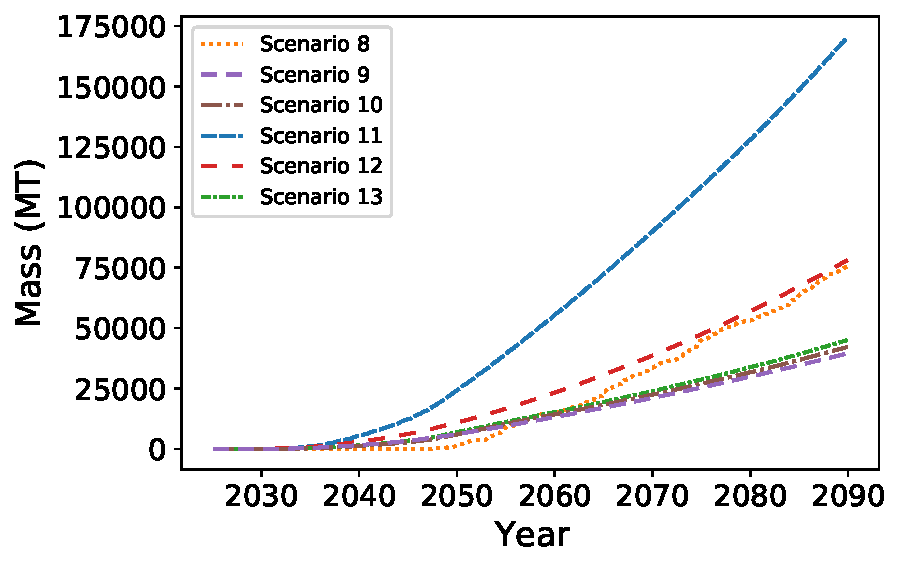
\includegraphics[width=\textwidth]{1percent_waste_cumulative.pdf}
        \caption{Cumulative mass of fuel discharged from advanced reactors 
        between 2025-2090.}
        \label{fig:1percent_waste_cumulative}
    \end{subfigure}
       \caption{Mass of fuel discharged from reactors 
       as a function of time for Scenarios 8-13. }
       \label{fig:1percent_waste}
\end{figure}

\begin{table}[h!]
    \centering 
    \caption{Metrics for waste discharged from advanced reactors 
    between 2025-2090 in Scenarios 8-13. The ``Average \gls{HALEU}''
    is the average mass of \gls{SNF} from \gls{HALEU}-fueled 
    reactors. }
    \label{tab:1percent_waste}
    \begin{tabular}{c c c c c}
        \hline
        Scenario & Average (MT/month) & Average of \gls{HALEU} (MT/month) 
        & Maximum (MT) & Cumulative (MT)\\\hline
        8 & 96.39 & 96.39 & 1,373 & 75,085 \\
        9 & 52.67 & 52.67 & 108.9 & 41,026 \\
        10 & 57.79 & 57.79 & 133.6 & 45,014 \\
        11 & 230.5 & 10.56 & 533.1 & 179,534 \\
        12 & 109.0 & 37.57 & 226.9 & 84,880 \\
        13 & 61.47 & 55.45 & 145.0 & 47,884 \\
        \hline
    \end{tabular}
\end{table}

Based on the cumulative masses, the proposed 70,000 MTHM capacity of 
a geologic repository in the US would only store the \gls{SNF} 
discharged from advanced reactors in Scenarios 8, 9, 10, and 13. Additional 
repositories or an expanded capacity of the repository would be required 
to dispose of the waste from Scenarios 11 and 12. The 
cumulative \gls{SNF} discharged from advanced reactors is less than the 
cumulative mass discharged from the \glspl{LWR} in all scenarios except 
Scenario 11. Scenario 11 discharges more \gls{SNF} because of the large 
number of VOYGRs it deploys to meet the increasing energy demand. 



\chapter{Recycling transition results} \label{ch:recycle_results}
This chapter reports the results for the recycle fuel cycle 
scenarios (Scenarios 14-19) described 
in Section \ref{sec:recycle-methods}. The primary results considered 
for these fuel cycle transitions are the uranium resources needed, 
the \gls{SWU} capacity required, the separated plutonium masses, 
and the mass of disposed material. This chapter does not focus 
on the number of reactors or the energy supplied by 
the reactors because most of the scenarios use the same 
deployment scheme as Scenarios 7 or 13 (depending on 
the energy demand curve of the scenario). For the two 
scenarios that deploy the \gls{SFR} instead of the other 
advanced reactors (Scenarios 16 and 19), the maximum number 
of \glspl{SFR} deployed in each scenario is 312 and 595, 
respectively. 
These scenarios require far fewer reactors than the other scenarios 
because the \gls{SFR} has a larger power output than the other 
advanced reactors (311 MWe compared with 80 MWe for the Xe-100).

\section{Uranium resources}
We divide the uranium resources described here into two primary 
components: the heavy metal mass and the natural uranium 
required to produce fuel. We further divide the heavy metal 
mass into two parts: the enriched uranium and the 
heavy metals in plutonium-based fuel (\gls{MOX} or U/TRU fuel). 
Enriched uranium is in the 
\gls{HALEU}, \gls{UOX}, and UCO fuels. Heavy metals in plutonium-based 
fuels include the natural uranium, plutonium, and transuranic 
elements in 
the \gls{MOX} and U/TRU fuels. We separate these metrics 
because of the different processes and resources needed to 
produce each fuel type. We also divide the natural uranium 
masses into two parts: the feed uranium to produce enriched uranium 
and the natural uranium required to produce 
plutonium-based fuel. Dividing this metric provides more details 
on the resources needed to support these fuel cycles. 

\subsection{No growth scenarios}
This section presents the results of the uranium resources required 
in the no growth, closed fuel cycle scenarios (Scenarios 14-16). 
We divide these results into the heavy metal masses (enriched uranium 
and heavy metals in plutonium-based fuel) and the natural 
uranium masses (feed uranium and natural uranium to produce 
plutonium-based fuels). We compare each of these material requirements 
based on monthly averages, maximum values, 
and cumulative masses. We also compare the enriched uranium and feed uranium 
masses based on the monthly average for \gls{HALEU}. 

\subsubsection{Heavy metal masses}
Figure \ref{fig:nogrowth_recycle_uranium} shows 
the mass of enriched uranium required by Scenarios 14-16. 
Scenario 15 requires the most enriched uranium, followed by 
Scenario 14, then Scenario 16. Scenario 15 requires the most enriched 
uranium because less material is available for reprocessing (no 
\gls{TRISO} spent fuel gets reprocessed), leading to 
less separated plutonium and less plutonium-based fuel available. The 
advanced reactors 
in these scenarios prefer plutonium-based fuel over uranium-based fuel, 
meaning that they will accept as much plutonium-based fuel that 
is available. 
Therefore, a larger supply of plutonium-based fuel means than less 
uranium-based fuel is needed to support these reactors.
The annual average mass of enriched uranium (Figure 
\ref{fig:nogrowth_recycle_AR_uranium}) in Scenarios 14 and 15 increases 
in 2043 because the plutonium-based fuel stockpiled up from 
reprocessed \gls{LWR} \gls{SNF} is used up and there is not as much 
plutonium from the advanced reactor \gls{SNF} to produce more 
plutonium-based fuel. 

\begin{figure}[h!]
    \centering
    \begin{subfigure}[b]{0.45\textwidth}
        \centering
        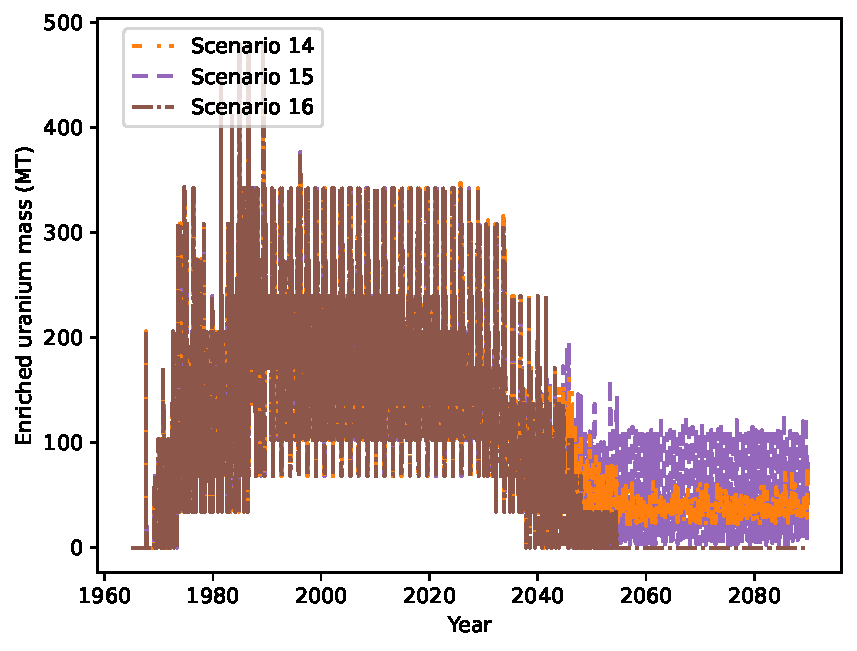
\includegraphics[width=\textwidth]{nogrowth_recycle_total_fuel.pdf}
        \caption{Monthly mass sent to all reactors 
        between 1965-2090.}
        \label{fig:nogrowth_recycle_all_uranium}
    \end{subfigure}
    \hfill
    \begin{subfigure}[b]{0.45\textwidth}
        \centering
        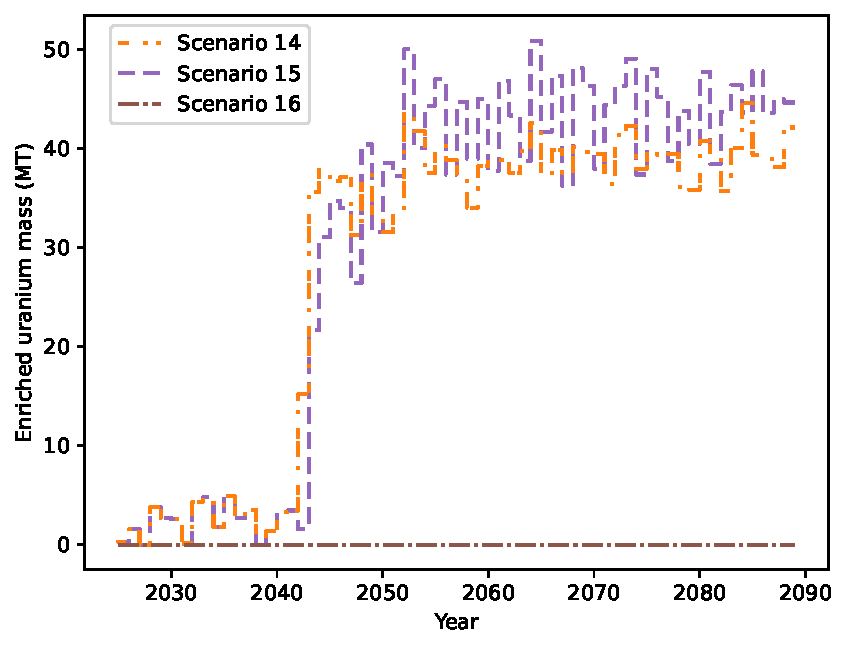
\includegraphics[width=\textwidth]{nogrowth_recycle_Uaverages.pdf}
        \caption{Annual average mass sent to 
        advanced reactors between 2025-2090.}
        \label{fig:nogrowth_recycle_AR_uranium}
    \end{subfigure}
    \begin{subfigure}[b]{0.45\textwidth}
        \centering
        \includegraphics[width=\textwidth]{nogrowth_recycle_Ucumulative.pdf}
        \caption{Cumulative mass sent to advanced reactors between 2025-2090.}
        \label{fig:nogrowth_recycle_uranium_cumulative}
    \end{subfigure}
       \caption{Mass of enriched uranium required by reactors
        in Scenarios 14-16.}
       \label{fig:nogrowth_recycle_uranium}
\end{figure}

Scenario 16 does not require any uranium-based fuel to support the 
advanced reactors. This result stems from a few key differences between 
Scenario 16 and the other no growth closed fuel cycle scenarios. The 
first difference is that all of the advanced 
reactors in Scenario 16 can accept reprocessed fuel, while the \glspl{MMR} 
in Scenarios 14 and 15 will only accept \gls{UOX}. This modeling 
decision for the \gls{MMR} means that any fuel cycle that 
deploys the \gls{MMR} will always require some amount of uranium-based 
fuel. Therefore, the lack of \gls{MMR} deployment in Scenario 16 allows 
the possibility for this scenario to not require enriched uranium if 
there is enough plutonium-based fuel to fuel the advanced reactors. 
The second difference is the reprocessing scheme.  
In Scenario 16, the spent fuel can be reprocessed an infinite number 
of times while in Scenarios 14 and 15 the spent uranium-based fuel can 
only be reprocessed once and the plutonium-based fuel can not be 
reprocessed. This difference is inherent to the type of fuel cycle 
(limited vs. continuous recycle), and increases the amount of 
\gls{SNF} available for reprocessing. Additionally, the reprocessing 
step in Scenario 16 removes the uranium, neptunium, plutonium, 
and americium from the spent fuel, compared with only plutonium 
being separated out in Scenarios 14 and 15. Allowing more material 
to be separated out of the \gls{SNF} in Scenario 16 leads to more 
separated actinide material to create the plutonium-based fuel. 

Table \ref{tab:s14-16_uranium} reports the average enriched uranium mass, 
average \gls{HALEU} mass, maximum enriched uranium mass, and cumulative 
enriched uranium mass required in Scenarios 14-16. Scenario 14 requires 
less enriched uranium than Scenario 7, despite having the same 
advanced reactor deployment schedule, because of the change in the 
fuel cycle. By reprocessing spent fuel, the average \gls{HALEU} 
mass required drops by 21.3\%. A similar decrease in cumulative 
\gls{HALEU} needs is seen in Scenario 15. However, the removal of 
\gls{TRISO} reprocessing results in a smaller decrease (15.1\%
decrease). By reprocessing the \gls{TRISO}-based fuels in 
Scenario 14, the reactors in this scenario needs 6.35\% less 
cumulative enriched uranium than the reactors in Scenario 15. 

\begin{table}[h!]
    \centering 
    \caption{Metrics for enriched uranium required to fuel reactors 
    in Scenarios 14-16.}
    \label{tab:s14-16_uranium}
    \begin{tabular}{c c c c c}
        \hline 
        Scenario & Average (MT/month) & HALEU Average (MT/month) 
        & Maximum (MT) & Cumulative (MT) \\
        \hline 
        14 & 28.01 & 27.16 & 87.01 & 21,920 \\
        15 & 30.05 & 29.20 & 143.8 & 23,407\\
        16 & 0 & 0 & 0 & 0\\
        \hline
        
    \end{tabular}
\end{table}

Scenarios 14, 15, and 16 require a cumulative enriched uranium 
mass of 3,162 MT, 2,667 MT, and 0 MT, respectively, by 2050. These values 
are smaller than the needs of the once-through fuel cycles 
(Table \ref{tab:nogrowth_haleu}) and the estimated 5,350 MT in 
a once-through fuel cycle from 
Dixon et al. \cite{dixon_estimated_2022}. The closed fuel cycle 
scenarios require less \gls{HALEU} than the once-through 
fuel cycles because of the inclusion of reprocessing and use 
of plutonium-based fuel in the advanced reactors. 

In addition to the enriched uranium, the advanced 
reactors receive heavy metals for the plutonium-based 
fuels. Figure 
\ref{fig:nogrowth_recycle_mox} shows that Scenario 16 requires more 
plutonium-based fuel than the other scenarios. This result is consistent 
with the reactors in Scenarios 16 not receiving any enriched 
uranium. Scenario 14 uses the next largest mass of heavy metals for 
plutonium-based fuel, followed by Scenario 15. 

\begin{figure}[h!]
    \centering
    \begin{subfigure}[b]{0.45\textwidth}
        \centering
        \includegraphics[width=\textwidth]{nogrowth_recycle_MOX.pdf}
        \caption{Monthly masses sent to 
        advanced reactors between 2025-2090.}
        \label{fig:nogrowth_recycle_AR_mox}
    \end{subfigure}
    \hfill
    \begin{subfigure}[b]{0.45\textwidth}
        \centering
        \includegraphics[width=\textwidth]{nogrowth_recycle_MOXcumulative.pdf}
        \caption{Cumulative mass 
        sent to advanced reactors between 2025-2090.}
        \label{fig:nogrowth_recycle_mox_cumulative}
    \end{subfigure}
       \caption{Mass of plutonium-based fuel required by reactors
        in Scenarios 14-16.}
       \label{fig:nogrowth_recycle_mox}
\end{figure}

As Table \ref{tab:s14-16_mox} reports, the average and cumulative 
masses of plutonium-based fuel heavy metals in Scenario 16 are an 
order of magnitude greater than the masses in Scenario 14-15. 
This large difference 
is a result of the different reprocessing schemes, as previously 
described. 
Scenario 16 needs a monthly average 
of plutonium-based fuel heavy metal that is more than the maximum mass 
needed in Scenario 14. More heavy metal for plutonium-based fuel
is sent to advanced reactors in Scenario 14 than  
in Scenario 15 because the reprocessing of \gls{TRISO} fuel in 
Scenario 14 increases the availability of 
plutonium-based fuel. The heavy metals for plutonium fuels 
in Scenarios 14 and 15 show a decrease in 2043, corresponding 
to the increase in enriched uranium sent to reactors in these 
scenarios. After the initial stock of plutonium-based fuel 
from \gls{LWR} spent fuel is used in Scenarios 14 and 15, these 
scenarios use an 
average of 5.26 MT/month and 1.49 MT/month of plutonium-based 
fuel, respectively. These 
values are both smaller than the average values reported 
in Table \ref{tab:s14-16_mox}, highlighting the importance 
of a stockpile of plutonium-based fuel from \gls{LWR} spent 
fuel in providing plutonium-based fuel for advanced reactors in these fuel 
cycles. 

\begin{table}[h!]
    \centering 
    \caption{Metrics for plutonium-based fuels required to fuel reactors 
    in Scenarios 14-16.}
    \label{tab:s14-16_mox}
    \begin{tabular}{c c c c}
        \hline 
        Scenario & Average (MT/month) & Maximum (MT) & Cumulative (MT) \\
        \hline 
        14 & 7.351 & 53.81 & 5,727 \\
        15 & 4.506 & 81.59 & 3,510 \\
        16 & 72.70 & 241.9 & 56,630 \\
        \hline
        
    \end{tabular}
\end{table}

When comparing the total cumulative mass of heavy metal (enriched 
uranium and heavy metal in plutonium-based fuel) required by each scenario,
Scenario 16 needs the most material of these three scenarios. This 
result stems from the different discharge burnups of the reactors. The 
\gls{SFR} has a burnup of 87.51 MWd/kg HM and the Xe-100 (the reactor that 
meets most of the demand in Scenarios 14 and 15) has a burnup of 168 MWd/kg U. 
The Xe-100 gets more energy out the fuel per unit mass, which leads to 
Scenarios 14 and 15 requiring less fuel than Scenario 16. Scenario 16 is most 
similar to Scenario 2 in the amount of heavy metals required, because
the \gls{SFR} and \gls{MMR} have similar discharge burnups (87.51 MWd/kg 
compared with 82.6 MWd/kg).

\subsubsection{Natural uranium}
Figure \ref{fig:nogrowth_recycle_feed} shows 
the natural uranium required as feed uranium to produce enriched 
uranium fuel for advanced reactors in Scenarios 14-16.  
Scenario 15 requires 
the most feed uranium, followed by Scenarios 14 and 16. This pattern follows 
with the enriched uranium mass in each scenario, because the enriched 
uranium mass dictates the amount of feed uranium needed.
Scenario 15 requires the 
most feed mass because less \gls{SNF} is available for reprocessing, 
leading to more 
enriched uranium required. Scenario 
16 does not requires any feed uranium because it does not require any 
enriched uranium. 

\begin{figure}[h!]
    \centering
    \begin{subfigure}[b]{0.45\textwidth}
        \centering
        \includegraphics[width=\textwidth]{nogrowth_recycle_feed.pdf}
        \caption{Monthly mass 
        to support all reactors between 1965-2090.}
        \label{fig:nogrowth_recycle_all_feed}
    \end{subfigure}
    \hfill
    \begin{subfigure}[b]{0.45\textwidth}
        \centering
        \includegraphics[width=\textwidth]{nogrowth_recycle_feed_average.pdf}
        \caption{Annual average  mass 
        to support advanced reactors between 2025-2090.}
        \label{fig:nogrowth_recycle_AR_feed}
    \end{subfigure}
    \begin{subfigure}[b]{0.45\textwidth}
        \centering
        \includegraphics[width=\textwidth]{nogrowth_recycle_feed_cumulative.pdf}
        \caption{Cumulative mass to support advanced reactors between 2025-2090.}
        \label{fig:nogrowth_recycle_feed_cumulative}
    \end{subfigure}
       \caption{Mass of feed uranium required by reactors
        in Scenarios 14-16.}
       \label{fig:nogrowth_recycle_feed}
\end{figure}

Table \ref{tab:s14-16_feed} reports the metrics for the feed uranium 
required in Scenarios 14-16. The cumulative feed uranium needed in 
Scenarios 14 and 15 are both less than the cumulative feed uranium 
needed in Scenario 7. The decrease in feed uranium needed demonstrates 
how using a closed fuel cycle can reduce the feed uranium needs in 
addition to reducing the fuel mass needs. 

\begin{table}[h!]
    \centering 
    \caption{Metrics for feed uranium required to produce 
    uranium-based fuels in in Scenarios 14-16.}
    \label{tab:s14-16_feed}
    \begin{tabular}{c c c c c}
        \hline 
        Scenario & Average (MT/month) & HALEU Average (MT/month) &
        Maximum (MT) & Cumulative (MT) \\
        \hline 
        14 & 842.9 & 836.4 & 2,628 & 656,582 \\
        15 & 903.9 & 897.4 & 4,450 & 704,106\\
        16 & 0 & 0 & 0 & 0\\
        \hline
        
    \end{tabular}
\end{table}

Next, Figure \ref{fig:nogrowth_recycle_natu} shows the natural 
uranium required for the plutonium-based fuels in Scenarios 14-16. 
These results follow the same pattern as the heavy metal for 
plutonium-based fuels in these scenarios (Figure 
\ref{fig:nogrowth_recycle_mox}). However, the natural 
uranium mass is less than the total heavy metal mass, because the 
uranium is only a part of the total heavy metal mass in plutonium-based 
fuel. Scenario 16 requires 
the most natural uranium because the reactors in this scenario 
only receive the U/TRU fuel. Scenario 15 requires the least 
natural uranium, because this scenario results in the least 
plutonium-based fuel.

\begin{figure}[h!]
    \centering
    \begin{subfigure}[b]{0.45\textwidth}
        \centering
        \includegraphics[width=\textwidth]{nogrowth_recycle_natU.pdf}
        \caption{Monthly mass to support
        advanced reactors between 2025-2090.}
        \label{fig:nogrowth_recycle_AR_natu}
    \end{subfigure}
    \hfill
    \begin{subfigure}[b]{0.45\textwidth}
        \centering
        \includegraphics[width=\textwidth]{nogrowth_recycle_natU_cumulative.pdf}
        \caption{Cumulative mass to support advanced reactors between 2025-2090.}
        \label{fig:nogrowth_recycle_natu_cumulative}
    \end{subfigure}
       \caption{Mass of natural uranium for plutonium-based fuel required 
       by reactors
        in Scenarios 14-16.}
       \label{fig:nogrowth_recycle_natu}
\end{figure}

Table \ref{tab:s14-16_natU} reports the metrics for the natural uranium 
required for Scenarios 14-16. The metrics for Scenario 16 are one order 
of magnitude greater than the metrics for Scenarios 14-15, the same as 
the metrics of the plutonium-based fuel heavy metal. 
The cumulative natural uranium mass 
needed by Scenario 16 is more than one order of magnitude smaller than 
the cumulative feed uranium masses in Scenarios 14 and 15, because of the 
difference in process losses in each use of natural uranium. Using natural 
uranium as fill material in plutonium-based fuel has relatively small 
process losses because the material is used in its direct form. However, 
using natural uranium as feed for enrichment has large material losses 
(referred to as the tails material stream)
because of the low enrichment of natural uranium (0.711\%). Based on 
Eq. \ref{eq:enrichment}, the process losses increase with increased 
product mass demand and with increased product assay. The different 
masses of natural uranium for use in plutonium-based fuel and 
for enrichment suggests that fuel cycle that maximizes 
the amount of plutonium-based fuel and minimizes the amount of 
enriched uranium required helps to minimize natural uranium requirements. 

\begin{table}[h!]
    \centering 
    \caption{Metrics for natural uranium required to produce 
    plutonium-based fuels in Scenarios 14-16.}
    \label{tab:s14-16_natU}
    \begin{tabular}{c c c c}
        \hline 
        Scenario & Average (MT/month) & Maximum (MT) & Cumulative (MT) \\
        \hline 
        14 & 6.256 & 45.80 & 4,874 \\
        15 & 3.835 & 69.44 & 2,987 \\
        16 & 55.68 & 185.3 & 43,372 \\
        \hline
        
    \end{tabular}
\end{table}

\subsection{1\% growth scenarios}
This section presents the results of the uranium resources required 
in the 1\% growth, closed fuel cycle scenarios (Scenarios 17-19). 
We divide these results into the fuel masses (enriched uranium 
and heavy metals in plutonium-based fuel) and the natural 
uranium masses (feed uranium and natural uranium to produce 
plutonium-based fuels).

\subsubsection{Fuel masses}
The first fuel mass considered is the enriched uranium mass, 
shown in Figure \ref{fig:1percent_recycle_uranium}. These results 
show the same pattern as this metric for the no growth scenarios:
Scenario 18 requires the most enriched uranium and Scenario 19 
does not require any enriched uranium. In Scenarios 17 and 18 the 
increase in enriched uranium need occurs closer to 2040 and is a 
more gradual increase than the observed increase in Scenarios 14-15. 
These results stem from differences in the growth in energy 
demand, and subsequent differences in reactor deployment, leading to the stockpile 
of plutonium-based fuel from \gls{LWR} \gls{SNF} to be used up sooner. 
The differences in energy demand and reactor deployment lead to different 
proportions of the advanced reactors, specifically the artificially
inflated number of \gls{MMR} deployed in these scenarios described 
in Section \ref{sec:1percent_reactors}. These differences 
lead to the more gradual increase in the enriched uranium needs
because of the slow increase in the number of \glspl{MMR} deployed.

\begin{figure}[h!]
    \centering
    \begin{subfigure}[b]{0.45\textwidth}
        \centering
        \includegraphics[width=\textwidth]{1percent_recycle_total_fuel.pdf}
        \caption{Monthly mass sent to all reactors 
        between 1965-2090.}
        \label{fig:1percent_recycle_all_uranium}
    \end{subfigure}
    \hfill
    \begin{subfigure}[b]{0.45\textwidth}
        \centering
        \includegraphics[width=\textwidth]{1percent_recycle_Uaverages.pdf}
        \caption{Annual average mass sent to 
        advanced reactors between 2025-2090.}
        \label{fig:1percent_recycle_AR_uranium}
    \end{subfigure}
    \begin{subfigure}[b]{0.45\textwidth}
        \centering
        \includegraphics[width=\textwidth]{1percent_recycle_Ucumulative.pdf}
        \caption{Cumulative mass sent to advanced reactors between 2025-2090.}
        \label{fig:1percent_recycle_uranium_cumulative}
    \end{subfigure}
       \caption{Mass of enriched uranium required by reactors
        in Scenarios 17-19.}
       \label{fig:1percent_recycle_uranium}
\end{figure}

Table \ref{tab:s17-19_enrichedU} reports the metrics for the enriched 
uranium masses for Scenarios 17-19. The cumulative enriched 
uranium in Scenarios 17 and 18 are less than the cumulative 
enriched uranium required by Scenario 13. However, the cumulative 
mass for Scenario 18 is larger than the cumulative in Scenario 
9. These results highlight how reprocessing can reduce enriched 
uranium needs, but the reactors deployed and their fuel usage 
is still an important factor in how much enriched uranium is 
needed. 

\begin{table}[h!]
    \centering 
    \caption{Metrics of enriched uranium fuel between 2025-2090 in Scenarios 
    17-19.}
    \label{tab:s17-19_enrichedU}
    \begin{tabular}{c c c c c}
        \hline 
        Scenario & Average (MT/month) & Average HALEU (MT/month) &  
        Maximum (MT) & Cumulative (MT) \\
        \hline
        17 & 58.72 & 52.81 & 152.2 & 45,742\\
        18 & 63.32 & 57.42 & 160.9 & 49,329\\
        19 & 0 & 0 & 0 & 0\\
        \hline
    \end{tabular}
\end{table}

Next is the mass of plutonium-based fuels sent to the advanced reactors 
in Scenarios 17-19, shown in Figure \ref{fig:1percent_recycle_mox}.
Similar to the patterns of the no growth scenarios, Scenario 19 
requires the most 
plutonium-based fuel of the three scenarios and Scenario 17 
requires more than Scenario 18. Scenarios 17 and 18 show the 
initial stockpile of plutonium-based fuel from \gls{LWR} \gls{SNF} that 
gets used by 2040. The plutonium-based fuel mass in Scenario 18 
drops to near zero after 2060, because all of the spent fuel from 
the \glspl{LWR} has been processed and used to create plutonium-based 
fuel, 
and there are so few VOYGRs (the only advanced reactor spent fuel 
reprocessed in this scenario) to produce more separated plutonium 
and more \gls{MOX}. The differences in the plutonium-based fuel 
heavy metal masses in these three scenarios is primarily 
a function of the reprocessing scheme of each scenario. 

\begin{figure}[h!]
    \centering
    \begin{subfigure}[b]{0.45\textwidth}
        \centering
        \includegraphics[width=\textwidth]{1percent_recycle_MOX.pdf}
        \caption{Monthly mass sent to all reactors 
        between 1965-2090.}
        \label{fig:1percent_recycle_AR_mox}
    \end{subfigure}
    \hfill
    \begin{subfigure}[b]{0.45\textwidth}
        \centering
        \includegraphics[width=\textwidth]{1percent_recycle_MOXcumulative.pdf}
        \caption{Cumulative mass  
        sent to advanced reactors between 2025-2090.}
        \label{fig:1percent_recycle_mox_cumulative}
    \end{subfigure}
       \caption{Masses of heavy metal in plutonium-based fuel 
        sent to advanced reactors
        in Scenarios 17-19.}
       \label{fig:1percent_recycle_mox}
\end{figure}

Table \ref{tab:s17-19_mox} reports the metrics for the
heavy metals in plutonium-based 
fuels required in Scenarios 17-19. Scenario 19 uses the largest 
heavy metal mass, followed by Scenario 17, then 18. 
Scenario 19 requires more total heavy metal (in enriched 
uranium and plutonium-based fuels) than Scenarios 
17 and 18, as well as Scenarios 9, 10, 12, and 13. Scenario 19 
uses the most similar cumulative mass of heavy metal as Scenario 8, 
because the \gls{MMR} and \gls{SFR} have the most similar burnups 
of the advanced reactors considered. However, Scenario 19 requires 
less heavy metal than Scenario 8 because the \gls{SFR} has a higher 
burnup than the \gls{MMR}. These results emphasize how the 
the reactors deployed play an important role in determining how 
much fuel is required for a fuel cycle.  

\begin{table}[h!]
    \centering 
    \caption{Metrics of plutonium-based fuel between 2025-2090 in Scenarios 
    17-19.}
    \label{tab:s17-19_mox}
    \begin{tabular}{c c c c}
        \hline 
        Scenario & Average (MT/month) & Maximum (MT) & Cumulative (MT) \\
        \hline
        17 & 10.25 & 62.56 & 7,987\\
        18 & 5.109 & 62.56 & 3,979\\
        19 & 126.2 & 318.7 & 98,323\\
        \hline
    \end{tabular}
\end{table}

\subsubsection{Natural uranium}
The next two metrics are related to the natural uranium requirements of 
Scenarios 17-19. The first of these two metrics is the 
natural uranium needed as feed material for enrichment, shown in 
Figure \ref{fig:1percent_recycle_feed}. The feed uranium masses follow with 
the enriched uranium masses in these scenarios, because of 
the relationship between these two metrics. Scenario 18 requires 
the most feed uranium, and Scenario 19 requires no feed uranium. 
There is increased demand for feed uranium with time in Scenarios 17 
and 18, resulting from the increased energy demand 
and the increased demand of uranium-based fuel in the scenarios.  

\begin{figure}[h!]
    \centering
    \begin{subfigure}[b]{0.45\textwidth}
        \centering
        \includegraphics[width=\textwidth]{1percent_recycle_feed.pdf}
        \caption{Monthly mass to support all reactors 
        between 1965-2090.}
        \label{fig:1percent_recycle_all_feed}
    \end{subfigure}
    \hfill
    \begin{subfigure}[b]{0.45\textwidth}
        \centering
        \includegraphics[width=\textwidth]{1percent_recycle_feed_average.pdf}
        \caption{Annual average mass to support
        advanced reactors between 2025-2090.}
        \label{fig:1percent_recycle_AR_feed}
    \end{subfigure}
    \begin{subfigure}[b]{0.45\textwidth}
        \centering
        \includegraphics[width=\textwidth]{1percent_recycle_feed_cumulative.pdf}
        \caption{Cumulative mass to support advanced reactors between 2025-2090.}
        \label{fig:1percent_recycle_feed_cumulative}
    \end{subfigure}
       \caption{Masses of feed uranium required by reactors
        in Scenarios 17-19.}
       \label{fig:1percent_recycle_feed}
\end{figure}

Table \ref{tab:s17-19_feed} reports the metrics for the feed uranium in 
Scenarios 17-19. Scenarios 17 and 18 need more feed uranium than 
Scenarios 9 and 12. Scenarios 9 and 12 primarily deploy the Xe-100,
while Scenarios 17 and 18 deploy an inflated number of \glspl{MMR}, 
because of the direct replacement of \glspl{MMR} in the deployment 
scheme. The inflated number of \glspl{MMR} increases the 
feed uranium requirements because the \glspl{MMR} only accept 
\gls{HALEU} fuel in these scenarios, and the \gls{MMR} requires 
more feed uranium per unit energy than the Xe-100. Scenario 19 does not 
require any feed uranium because the \glspl{SFR} in this scenario 
only receive plutonium-based fuel. 

\begin{table}[h!]
    \centering 
    \caption{Metrics of feed uranium to produce enriched uranium 
    between 2025-2090 in Scenarios 17-19.}
    \label{tab:s17-19_feed}
    \begin{tabular}{c c c c c}
        \hline 
        Scenario & Average (MT/month) & HALEU Average (MT/month) & 
        Maximum (MT) & Cumulative (MT) \\
        \hline
        17 & 1,774 & 1,728 & 4,750 & 1,381,600\\
        18 & 1,866 & 1,911 & 5,014 & 1,489,022\\
        19 & 0 & 0 & 0 & 0\\
        \hline
    \end{tabular}
\end{table}

Finally, Figure \ref{fig:1percent_recycle_natU} shows the natural uranium 
required to produce plutonium-based fuels in Scenarios 17-19. Scenario 
19 requires the most natural uranium for plutonium-based fuels, 
followed by Scenario 17, then Scenario 18. The masses of plutonium-based 
fuel drives the demand for this natural uranium, therefore these 
results follow the same patterns seen in Figure \ref{fig:1percent_recycle_mox}.
Scenario 19 requires the most natural uranium for plutonium-based 
fuels because the advanced reactors in this scenario only receive 
plutonium-based fuel, and the \gls{SFR} requires more fuel than 
the Xe-100. 

\begin{figure}[h!]
    \centering
    \begin{subfigure}[b]{0.45\textwidth}
        \centering
        \includegraphics[width=\textwidth]{1percent_recycle_natU.pdf}
        \caption{Monthly mass to support advanced reactors 
        between 1965-2090.}
        \label{fig:1percent_recycle_AR_natu}
    \end{subfigure}
    \hfill
    \begin{subfigure}[b]{0.45\textwidth}
        \centering
        \includegraphics[width=\textwidth]{1percent_recycle_natU_cumulative.pdf}
        \caption{Cumulative mass to support
        advanced reactors between 2025-2090.}
        \label{fig:1percent_recycle_natu_cumulative}
    \end{subfigure}
       \caption{Mass of natural uranium required by reactors in 
       plutonium-based fuels in Scenarios 17-19.}
       \label{fig:1percent_recycle_natU}
\end{figure}

Table \ref{tab:s17-19_natU} reports the metrics for the 
natural uranium for plutonium-based fuels in Scenarios 17-19. 
These metric follow the same pattern observed for the 
no growth scenarios (Scenarios 14-16). Despite Scenario 19 
requiring the most natural uranium for plutonium-based 
fuels, this total is still less than the cumulative feed uranium 
masses required in Scenarios 17 and 18 by almost a factor 
of two. The decreased total 
natural uranium mass in Scenario 19, compared with Scenarios 
17 and 18, is a result of the lack of (or minimal) material loss in 
using natural uranium for plutonium-based fuel, compared with 
the losses from using natural uranium as feed material for 
enrichment. 

\begin{table}[h!]
    \centering 
    \caption{Metrics of natural uranium required to produce 
    plutonium-based fuel between 2025-2090 in Scenarios 
    17-19.}
    \label{tab:s17-19_natU}
    \begin{tabular}{c c c c}
        \hline 
        Scenario & Average (MT/month) & Maximum (MT) & Cumulative (MT) \\
        \hline
        17 & 8.726 & 53.24 & 6,797\\
        18 & 4.348 & 53.24 & 3,387\\
        19 & 96.67 & 244.1 & 75,303\\
        \hline
    \end{tabular}
\end{table}


\section{SWU capacity}
The next category of metrics of interest is the \gls{SWU} capacity required 
to produce the enriched uranium in each of the scenarios. The \gls{SWU} 
capacity has important implications on the design and capacities of 
enrichment facilities required to support these fuel cycles. 

\subsection{No growth scenarios}
Figure \ref{fig:nogrowth_recycle_swu} shows \gls{SWU} capacity required 
in Scenarios 14-16. For Scenarios 14 and 15 the required \gls{SWU} 
capacity for the advanced reactors is relatively small, then increases 
around 2043, corresponding with the increased need for enriched uranium 
for reactors observed in Figure \ref{fig:nogrowth_recycle_uranium}. Scenario 
16 does not require any \gls{SWU} capacity because the advanced reactors 
in this scenario do not receive any enriched uranium. 

\begin{figure}[h!]
    \centering
    \begin{subfigure}[b]{0.45\textwidth}
        \centering
        \includegraphics[width=\textwidth]{nogrowth_recycle_swu.pdf}
        \caption{Monthly capacity to support all reactors between 2025-2090.}
        \label{fig:nogrowth_recycle_swu_all}
    \end{subfigure}
    \hfill
    \begin{subfigure}[b]{0.45\textwidth}
        \centering
        \includegraphics[width=\textwidth]{nogrowth_recycle_AR_swu.pdf}
        \caption{Annual average capacity to support advanced reactors between 2025-2090.}
        \label{fig:nogrowth_recycle_swu_AR}
    \end{subfigure}
       \caption{\gls{SWU} capacity required to support 
       reactors in Scenarios 14-16.}
       \label{fig:nogrowth_recycle_swu}
\end{figure}

Table \ref{tab:s14-16_swu} reports the metrics of required \gls{SWU} 
capacity in Scenarios 14-16. Scenarios 14 and 15 require smaller 
average \gls{SWU} capacities than Scenarios 2-7, and require a 
smaller average \gls{SWU} capacity to produce \gls{HALEU} than 
Scenarios 2, 3, 4, 6, and 7. Scenario 5 requires less \gls{SWU} 
capacity to produce \gls{HALEU} because this scenario 
primarily deploys VOYGRs and requires less \gls{HALEU} than 
any of the no growth scenarios that require \gls{HALEU}. 
The differences in the 
\gls{SWU} capacity needed by these scenarios is a function of 
the reactors deployed and the amount of material available for 
reprocessing. These parameters drive the amount of enriched 
uranium needed in each scenario, which drives the needed 
\gls{SWU} capacity.

\begin{table}[h!]
    \centering 
    \caption{Metrics for \gls{SWU} capacity required to produce 
    enriched uranium in Scenarios 14-16.}
    \label{tab:s14-16_swu}
    \begin{tabular}{c c c c}
        \hline 
        Scenario & Average (MT-SWU/month) & HALEU Average (MT-SWU/month)
         & Maximum (MT-SWU) \\
        \hline 
        14 & 971.6 & 965.9 & 3,032 \\
        15 & 1,042 & 1,036 & 5,142 \\
        16 & 0 & 0 & 0 \\
        \hline
        
    \end{tabular}
\end{table}

The results of these scenarios identify recycling \gls{SNF} as a way 
to reduce the \gls{SWU} capacity required in a fuel cycle. Additionally, 
increasing the amount of \gls{SNF} available for reprocessing further 
reduces the \gls{SWU} capacity required. The lack of needed 
\gls{SWU} capacity in Scenario 16 indicates that developing this 
fuel cycle would not require any new enrichment capacity to be developed 
in the US.  However, the US does not have 
any facilities for reprocessing commercial fuel. Therefore, reprocessing
fuel does not assist in meeting initial \gls{HALEU} demand because 
the US would need to develop new infrastructure to support any 
of these transitions, whether it is enrichment facilities, 
reprocessing facilities, or both. Advanced reactors in Scenarios 14 and 15 
require enriched uranium fuel, including \gls{HALEU}. These scenarios 
require a smaller \gls{HALEU} \gls{SWU} capacity than the once-through 
scenarios, but the US would need to develop \gls{HALEU} enrichment 
and reprocessing facilities to support these transitions. 

\subsection{1\% growth scenarios}
Figure \ref{fig:1percent_recycle_swu} shows the \gls{SWU} capacity 
required to enrich uranium in Scenarios 17-19. Similar to the 
feed uranium masses, the mass of enriched uranium drives 
the required \gls{SWU} capacity. Scenario 18 requires the most 
\gls{SWU} capacity, followed by Scenario 17, and Scenario 19 does 
not need any \gls{SWU} capacity to support the advanced reactors. 

\begin{figure}[h!]
    \centering
    \begin{subfigure}[b]{0.45\textwidth}
        \centering
        \includegraphics[width=\textwidth]{1percent_recycle_swu.pdf}
        \caption{Monthly SWU capacity to support all reactors between 2025-2090.}
        \label{fig:1percent_recycle_swu_all}
    \end{subfigure}
    \hfill
    \begin{subfigure}[b]{0.45\textwidth}
        \centering
        \includegraphics[width=\textwidth]{1percent_recycle_AR_swu.pdf}
        \caption{Annual average SWU capacity to support 
        advanced reactors between 2025-2090.}
        \label{fig:1percent_recycle_swu_AR}
    \end{subfigure}
       \caption{\gls{SWU} capacity required to support reactors in Scenarios 14-16.}
       \label{fig:1percent_recycle_swu}
\end{figure}

Table \ref{tab:s17-19_swu} reports the metrics for the \gls{SWU} capacities 
required in Scenarios 17-19. Scenarios 17 and 18 require less 
\gls{SWU} capacity than Scenario 13, because the use of 
reprocessing and plutonium-based fuel decreases the need for 
enriched uranium. Scenarios 17 and 18 require more \gls{SWU} 
capacity than Scenarios 9 and 12, because of the difference in 
the advanced reactors deployed between these scenarios. These results 
vary from the results of the no growth scenarios, in which the 
average \gls{SWU} of the closed fuel cycles were smaller than the 
average capacity in the once-through fuel cycles. This difference 
between the energy demand curves is a result of the deployment 
scheme artificially inflating the number of \glspl{MMR} built. This 
extra deployment of \glspl{MMR} in the 1\% growth scenarios that 
deploy the \gls{MMR} increases the \gls{SWU} capacity because the 
\gls{MMR} requires more enriched uranium and a higher enrichment 
level than the Xe-100 and VOYGR. Therefore, the deployment scheme 
of the reactors affects the metrics of the transition when changing 
the energy demand. 

\begin{table}[h!]
    \centering 
    \caption{Metrics for \gls{SWU} capacity required to produce 
    enriched uranium in Scenarios 17-19.}
    \label{tab:s17-19_swu}
    \begin{tabular}{c c c c}
        \hline 
        Scenario & Average (MT-SWU/month) & HALEU Average (MT-SWU/month)
         & Maximum (MT-SWU) \\
        \hline 
        17 & 2,049 & 2,009 & 5,504 \\
        18 & 2,207 & 2,168 & 5,806 \\
        19 & 0 & 0 & 0 \\
        \hline
        
    \end{tabular}
\end{table}

\section{Separated actinide mass}
The next metric of interest is the separated actinide mass sent 
from the separations facility to the fuel fabrication facility. 
The separated actinide masses include any actinides separated 
from \gls{SNF} (i.e., uranium, neptunium, plutonium, and 
americium). 
This metric provides context on how much material is available for 
producing plutonium-based fuels, and has implications on 
separations and fabrication facility size needs. Separations facilities 
are deployed starting in 2020, so these results begin in 2020 instead 
of 2025 like the other results. 

\subsection{No growth scenarios}
Figure \ref{fig:nogrowth_recycle_sep_pu} shows the separated plutonium 
masses in Scenarios 14-16. Scenario 16 has the most separated 
plutonium of the three scenarios, which is consistent with the other 
results of these scenarios. Scenarios 14 and 15 have very little 
separated plutonium compared with Scenario 16. The primary reason 
for this large difference is the elements separated out in 
each scenario. In Scenario 16, four different actinide elements 
are separated out from the fission products (uranium, neptunium,
plutonium, and americium), but in Scenarios 14 and 15 only plutonium 
is separated out. The inclusion of other elements to separate out 
in Scenario 16 (primarily the uranium, which consists of up to 
93\% of \gls{SNF}), increases the mass of material  
separated out from the \gls{SNF}. 

\begin{figure}[h!]
    \centering
    \begin{subfigure}[b]{0.49\textwidth}
        \centering
        \includegraphics[width=\textwidth]{nogrowth_recycle_sep_pu.pdf}
        \caption{Monthly mass between 2020-2090.}
        \label{fig:nogrowth_recycle_sep_pu_all}
    \end{subfigure}
    \hfill
    \begin{subfigure}[b]{0.49\textwidth}
        \centering
        \includegraphics[width=\textwidth]{nogrowth_recycle_sep_pu_cumulative.pdf}
        \caption{Cumulative mass between 2020-2090.}
        \label{fig:nogrowth_recycle_sep_pu_cumulative}
    \end{subfigure}
       \caption{Mass of separated actinides sent from the 
       separations facility to fuel fabrication in Scenarios 14-16.}
       \label{fig:nogrowth_recycle_sep_pu}
\end{figure}

Table \ref{tab:s14-16_sep_pu} reports the metrics of the separated 
actinide masses in Scenarios 14-16. All three scenarios experience a 
maximum amount of separated actinides at the same time, in 
November 2031. This timing corresponds with \gls{SNF} discharged 
from \glspl{LWR} in November 2025 and fuel from advanced reactors
discharged in October 2031. This consistency in the maximum 
for these three scenarios emphasizes the importance of reprocessing 
the \gls{SNF} from \glspl{LWR} in these metrics.  

\begin{table}[h!]
    \centering 
    \caption{Metrics of separated actinide masses of between 2020-2090 in 
    Scenarios 14-16.}
    \label{tab:s14-16_sep_pu}
    \begin{tabular}{c c c c}
        \hline 
        Scenario & Average (MT/month) & Maximum (MT) & Cumulative (MT) \\
        \hline
        14 & 1.372 & 4.735 & 1,150\\
        15 & 0.840 & 4.735 & 705.0\\
        16 & 140.1 & 454.3 & 117,584\\
        \hline
    \end{tabular}
\end{table}

From the metrics in Table \ref{tab:s14-16_sep_pu}, the metrics for 
the separated actinide masses in Scenario 16 are two orders of 
magnitude greater than the metrics in Scenarios 14 and 15. The metrics 
for Scenario 16 are also larger than the plutonium-based fuel metrics 
for the scenario in Table \ref{tab:s14-16_mox}. The larger mass 
of separated actinide material than plutonium-based fuels required by 
the reactors drives the lack of enriched uranium to support these 
reactors. The difference between the two material streams stems 
from the reprocessing of uranium from \gls{LWR} fuel, which constitutes 
about 93\% of the \gls{LWR} \gls{SNF}. Therefore, reprocessing 
uranium from \gls{LWR} \gls{SNF} plays an important role in supporting 
this fuel cycle. Between 2060-2090 (after all spent fuel from 
\glspl{LWR} is processed) the \glspl{SFR} require an 
average of 90.3 MT/month of U/TRU fuel, and an average of 95.2 
MT/month of separated actinides. Therefore, the \gls{SFR} could 
still sustain producing enough plutonium-based 
fuel from reprocessing \gls{SFR} \gls{SNF}.

Scenario 16 models the reprocessed uranium as being part of 
the fresh reprocessed fuel. Therefore, it is likely that 
fabricating the reprocessed fuel would not need the natural
uranium masses defined in Table \ref{tab:s14-16_natU}. If this 
production method is possible, then the natural uranium needs 
of the fuel cycle would drop to near-zero, further 
emphasizing how a closed fuel cycle can help minimize
natural uranium needs. 

In these fuel cycles, we model the Xe-100, VOYGR, and \gls{SFR} 
through the OpenMCyclus archetype, instead of using the 
\Cycamore \texttt{Reactor} like in the once-through scenarios. 
The comparison between OpenMCyclus 
and the \Cycamore \texttt{Reactor} (Section \ref{sec:benchmark})
shows that the \Cycamore \texttt{Reactor} yields larger separated 
plutonium masses than OpenMCyclus. Therefore, using the \Cycamore 
\texttt{Reactor} would potentially overestimate the amount of 
separated actinide material, which would overestimate the 
amount of plutonium-based fuel for the advanced reactors. 
Therefore, by using OpenMCyclus for the reactors that 
receive plutonium-based fuel in the closed fuel cycles, we can 
expect that the separated actinide and plutonium-based fuel masses are 
more accurate than if we used the \Cycamore \texttt{Reactor} 
archetype. 

\subsection{1\% growth scenarios}
Figure \ref{fig:1percent_recycle_sep_pu} shows the mass of separated 
actinide material in Scenarios 17-19. Similar to the no growth 
scenarios, Scenario 19 has a much greater mass of separated 
actinide material than Scenarios 17 and 18. The greater mass in 
Scenario 19 is a result of multiple actinide elements being 
separated out from the \gls{SNF}, compared with only 
plutonium separated in Scenarios 17 and 18, as well as more fuel 
being reprocessed in Scenario 19. 

\begin{figure}[h!]
    \centering
    \begin{subfigure}[b]{0.49\textwidth}
        \centering
        \includegraphics[width=\textwidth]{1percent_recycle_sep_pu.pdf}
        \caption{Mass 
        at each time step between 2020-2090.}
        \label{fig:1percent_recycle_sep_pu_all}
    \end{subfigure}
    \hfill
    \begin{subfigure}[b]{0.49\textwidth}
        \centering
        \includegraphics[width=\textwidth]{1percent_recycle_sep_pu_cumulative.pdf}
        \caption{Cumulative mass 
        at each time step between 2020-2090.}
        \label{fig:1percent_recycle_sep_pu_cumulative}
    \end{subfigure}
       \caption{Separated plutonium masses in Scenarios 17-19.}
       \label{fig:1percent_recycle_sep_pu}
\end{figure}

Table \ref{tab:s17-19_sep_pu} reports the metrics of the separated 
actinide masses on Scenarios 17-19. Scenarios 17 and 18 have the 
maximum separated plutonium mass in November 2031, the same time 
as the maximum in Scenarios 14 and 15. The consistency in the 
maximum separated actinide mass in all four of the limited 
recycle scenarios emphasizes the importance of reprocessing the 
\gls{LWR} \gls{SNF} in these scenarios. 

\begin{table}[h!]
    \centering 
    \caption{Mass of separated plutonium between 2020-2090 in Scenarios 
    17-19.}
    \label{tab:s17-19_sep_pu}
    \begin{tabular}{c c c c}
        \hline 
        Scenario & Average (MT/month) & Maximum (MT) & Cumulative (MT) \\
        \hline
        17 & 1.715 & 4.735 & 1,439\\
        18 & 0.854 & 4.735 & 716.4\\
        19 & 175.0 & 500.0 & 146,837\\
        \hline
    \end{tabular}
\end{table}

Figure 
\ref{fig:recycle_sep_pu} shows the annual average and cumulative 
separated actinide mass in Scenarios 14, 15, 17, and 18. All four of 
these scenarios have the same separated actinide masses until 
November 2028, Scenarios 14 and 15 have the same separated actinide 
mass until November 2041, and Scenarios 17 and 18 have the same separated 
actinide mass until February 2042. The similarities between these four 
scenarios is a result of the \gls{LWR} \gls{SNF} driving the amount 
of available separated actinide material, and the use of the 
same advanced reactor build share for scenarios of the same growth. 
However, the fuel considered for reprocessing has a greater impact 
on the amount of separated actinide material available than the 
energy demand. Scenarios 15 and 18 differ by a maximum of 41 kg of 
separated actinide material for a single time step, while Scenarios 
14 and 17 differ by a maximum of 1.4 MT in a single time step. 

\begin{figure}[h!]
    \centering
    \begin{subfigure}[b]{0.49\textwidth}
        \centering
        \includegraphics[width=\textwidth]{sep_pu_compare.pdf}
        \caption{Annual average mass between 2020-2090.}
        \label{fig:_recycle_sep_pu_all}
    \end{subfigure}
    \hfill
    \begin{subfigure}[b]{0.49\textwidth}
        \centering
        \includegraphics[width=\textwidth]{sep_pu_compare_cumulative.pdf}
        \caption{Cumulative mass between 2020-2090.}
        \label{fig:recycle_sep_pu_cumulative}
    \end{subfigure}
       \caption{Separated plutonium masses in the limited 
       recycle fuel cycles, Scenarios 14, 15, 17,18.}
       \label{fig:recycle_sep_pu}
\end{figure}

\section{Spent nuclear fuel and high level waste}
This section provides the results of the \gls{SNF} and \gls{HLW} sent 
to disposal in the closed fuel cycles. The once-through scenario 
results only defined the \gls{SNF} sent for disposal because all 
of the materials needing disposal in those scenarios are \gls{SNF}. 
With the addition of the separation step, the \gls{SNF} discharged 
from reactors gets separated into two different material streams, 
one of the separated plutonium and one of \gls{HLW} that is sent 
for disposal. \gls{SNF} 
is the spent fuel from each of the reactors that is disposed 
with reprocessing. \gls{HLW} is 
the waste (e.g., fission products) separated out from the 
reprocessed \gls{SNF}. 

\subsection{No growth scenarios}
This section presents the results of the \gls{SNF} and 
\gls{HLW} masses that are sent for disposal in a 
material sink in the no growth recycle scenarios. 

\subsubsection{Spent nuclear fuel}
Figure \ref{fig:nogrowth_recycle_snf} shows the 
masses of advanced reactor \gls{SNF} disposed of 
in Scenarios 14-16. In Scenario 14 only the spent \gls{MOX} 
fuel is disposed of, in Scenario 15 the spent \gls{MOX} as 
well as the spent \gls{TRISO}-based \gls{MMR} and Xe-100 fuels 
are disposed of, 
and no \gls{SNF} is disposed of in Scenario 16. The disposal of 
\gls{MMR} \gls{SNF} in Scenario 15 leads to the single times 
with larger disposal masses, because of the single-batch 
fueling scheme of the \gls{MMR}. The additional fuel that 
is disposed of in Scenario 15, compared with Scenarios 
14 and 16, increases the amount of \gls{SNF} disposed. 

\begin{figure}[h!]
    \centering
    \begin{subfigure}[b]{0.49\textwidth}
        \centering
        \includegraphics[width=\textwidth]{nogrowth_recycle_snf.pdf}
        \caption{Monthly mass sent for disposal 
        at each time step between 2025-2090.}
        \label{fig:nogrowth_recycle_snf_all}
    \end{subfigure}
    \hfill
    \begin{subfigure}[b]{0.49\textwidth}
        \centering
        \includegraphics[width=\textwidth]{nogrowth_recycle_snf_cumulative.pdf}
        \caption{Cumulative mass sent for disposal 
        at each time step between 2025-2090.}
        \label{fig:nogrowth_recycle_snf_cumulative}
    \end{subfigure}
       \caption{Spent nuclear fuel disposed of in Scenarios 14-16.}
       \label{fig:nogrowth_recycle_snf}
\end{figure}

Table \ref{tab:s14-16_snf} reports the metrics for the \gls{SNF} disposal 
in Scenarios 14-16. The values in this table are smaller than 
the \gls{SNF} masses in the once-through scenarios (Table 
\ref{tab:nogrowth_waste}). This decrease in \gls{SNF} disposal is 
a result of the reprocessing in Scenarios 14-16, and is an 
advantage of a closed fuel cycle. 

\begin{table}[h!]
    \centering 
    \caption{Mass of SNF disposed of between 2025-2090 in 
    Scenarios 14-16.}
    \label{tab:s14-16_snf}
    \begin{tabular}{c c c c}
        \hline 
        Scenario & Average (MT/month) & Maximum (MT) & Cumulative (MT) \\
        \hline
        14 & 7.835 & 41.33 & 6,103\\
        15 & 32.29 & 145.4 & 25,153 \\
        16 & 0 & 0 & 0 \\
        \hline
    \end{tabular}
\end{table}

Based on these values and the results in 
Figure \ref{fig:nogrowth_recycle_snf}, including more fuel for 
reprocessing can greatly reduce the mass of \gls{SNF}. All three of 
these scenarios have a cumulative \gls{SNF} mass smaller than 
that of all of the once-through scenarios. Additionally, 
the \gls{SNF} from advanced reactors in all three of these scenarios 
is less than the 70,000 MT limit for Yucca Mountain. The reduction in 
\gls{SNF} mass compared with the once-through scenarios highlights 
an advantage of closed fuel cycles. 

\subsubsection{High level waste}
Figure \ref{fig:nogrowth_recycle_hlw} shows the 
\gls{HLW} masses for disposal in Scenarios 14-16. Scenario 
14 results in the most \gls{HLW}, because more 
material is reprocessed in this scenario than in Scenario 15, 
and less actinide material is separated out than in 
Scenario 16. The \gls{HLW} mass in Scenario 15 reaches a 
near-zero level around 2060, because all of the \gls{LWR} 
\gls{SNF} is reprocessed by this time which leaves only
the VOYGR \gls{SNF} available for reprocessing. A 
maximum of 7 VOYGRs are deployed at a time in Scenario 
15, so there is very little \gls{SNF} reprocessed and 
little \gls{HLW} generated after 2060. 

\begin{figure}[h!]
    \centering
    \begin{subfigure}[b]{0.49\textwidth}
        \centering
        \includegraphics[width=\textwidth]{nogrowth_recycle_hlw.pdf}
        \caption{Monthly mass sent for disposal 
        at each time step between 2025-2090.}
        \label{fig:nogrowth_recycle_hlw_all}
    \end{subfigure}
    \hfill
    \begin{subfigure}[b]{0.49\textwidth}
        \centering
        \includegraphics[width=\textwidth]{nogrowth_recycle_hlw_cumulative.pdf}
        \caption{Cumulative mass sent for disposal 
        at each time step between 2025-2090.}
        \label{fig:nogrowth_recycle_hlw_cumulative}
    \end{subfigure}
       \caption{Mass of \gls{HLW} disposed of in Scenarios 14-16.}
       \label{fig:nogrowth_recycle_hlw}
\end{figure}

Table \ref{tab:s14-16_hlw} reports the metrics for the \gls{HLW} 
in Scenarios 14-16. Scenario 16 generates very little 
\gls{HLW} because the actinide material separated out 
comprises most of the mass of the \gls{SNF}. The \gls{HLW} 
masses for Scenarios 14 and 15 are larger than the \gls{SNF} 
masses for these scenarios, and are larger than the \gls{SNF} 
masses of the no growth, once-through scenarios, except 
Scenario 5. The increase 
comes from the inclusion of \gls{LWR} \gls{SNF} for reprocessing 
in these scenarios. Including this \gls{SNF} increases the 
disposed material mass because this metric is not solely focused 
on material from the advanced reactors like it was for 
the once-through scenarios. The average for 
Scenario 14 is similar to the average \gls{SNF} disposed of 
between 2025-2055 in Scenario 1 (94.27 MT/month). 

\begin{table}[h!]
    \centering 
    \caption{Mass of HLW disposed of between 2025-2090 in 
    Scenarios 14-16.}
    \label{tab:s14-16_hlw}
    \begin{tabular}{c c c c}
        \hline 
        Scenario & Average (MT/month) & Maximum (MT) & Cumulative (MT) \\
        \hline
        14 & 94.21 & 440.2 & 73,389\\
        15 & 67.73 & 440.2 & 52,764\\
        16 & 5.011 & 10.09 & 3,903\\
        \hline
    \end{tabular}
\end{table}

The \gls{HLW} in each of these scenarios has a different 
composition than the \gls{SNF}, but both waste streams 
still require a geologic repository for final 
disposal. Therefore, both the \gls{SNF} and \gls{HLW} 
masses must be considered for evaluating repository 
capacities. The \gls{HLW} in Scenario 14 is more than 
the 70,000 MT limit of Yucca Mountain, so a second 
repository would be needed to disposal of both waste 
streams. The \gls{SNF} and \gls{HLW} materials in 
Scenario 15 sum to 77,917 MT, meaning that a second 
repository would be needed to support this scenario 
as well. These material streams sum to 3,903 MT in 
Scenario 16, which means that the Yucca Mountain 
limit of 70,000 MT would be sufficient to support this 
scenario. 


\subsection{1\% growth scenarios}
This section presents the results of the \gls{SNF} and 
\gls{HLW} masses that are sent for disposal in a 
material sink in the 1\% growth recycle scenarios. 

\subsubsection{Spent nuclear fuel}
Figure \ref{fig:nogrowth_recycle_snf} shows the mass of \gls{SNF} 
disposed of in Scenarios 17-19. These results follow a similar 
pattern to the no growth scenarios; Scenario 18 disposes of 
the most \gls{SNF}, followed by Scenario 17, and Scenario 
19 does not have any \gls{SNF} disposed of. This pattern 
emerges because of the material available for reprocessing 
in each scenario. The more \gls{SNF} reprocessed, the less 
\gls{SNF} disposed. 

\begin{figure}[h!]
    \centering
    \begin{subfigure}[b]{0.49\textwidth}
        \centering
        \includegraphics[width=\textwidth]{1percent_recycle_snf.pdf}
        \caption{Monthly mass between 2025-2090.}
        \label{fig:1percent_recycle_snf_all}
    \end{subfigure}
    \hfill
    \begin{subfigure}[b]{0.49\textwidth}
        \centering
        \includegraphics[width=\textwidth]{1percent_recycle_snf_cumulative.pdf}
        \caption{Cumulative mass between 2025-2090.}
        \label{fig:1percent_recycle_snf_cumulative}
    \end{subfigure}
       \caption{Spent nuclear fuel disposed of in Scenarios 17-19.}
       \label{fig:1percent_recycle_snf}
\end{figure}

Table \ref{tab:s17-19_snf} reports the metrics of the \gls{SNF} 
disposed of in Scenarios 17-19. Scenarios 17 and 19 dispose of 
less \gls{SNF} than Scenarios 8-13, but Scenario 18 disposes of 
more \gls{SNF} than Scenario 9. Scenario 9 only deploys the 
Xe-100, while Scenario 18 has an artificially inflated number of 
\glspl{MMR} deployed, and the Xe-100 uses less fuel than the 
\gls{MMR}. We observe this effect in Scenario 18 and not 
Scenario 17, because \gls{MMR} \gls{SNF} is reprocessed in 
Scenario 17 but not in Scenario 18. Therefore the \gls{MMR} 
\gls{SNF} in Scenario 17 get split between the 
\gls{HLW} and plutonium-based fuel material streams. The \gls{SNF} mass comparisons 
between the closed and once-through fuel cycles are consistent 
with the other results: reprocessing fuel reduces material metrics, 
but the reactors deployed are the primary driver of the metrics. 

\begin{table}[h!]
    \centering 
    \caption{Mass of SNF disposed of between 2025-2090 in 
    Scenarios 17-19.}
    \label{tab:s17-19_snf}
    \begin{tabular}{c c c c}
        \hline 
        Scenario & Average (MT/month) & Maximum (MT) & Cumulative (MT) \\
        \hline
        17 & 9.542 & 35.47 & 7,433\\
        18 & 55.34 & 157.4 & 43,113\\
        19 & 0 & 0 & 0 \\
        \hline
    \end{tabular}
\end{table}


\subsubsection{High level waste}
Finally, Figure \ref{fig:1percent_recycle_hlw} shows the \gls{HLW} 
mass disposed of in Scenarios 17-19. These results are similar to 
the results from the no growth closed fuel cycle scenarios; Scenario 
17 has the most \gls{HLW} mass, followed by Scenario 18, and Scenario 
19. 
\begin{figure}[h!]
    \centering
    \begin{subfigure}[b]{0.49\textwidth}
        \centering
        \includegraphics[width=\textwidth]{1percent_recycle_hlw.pdf}
        \caption{Monthly mass of HLW sent for disposal 
        at each time step between 2025-2090.}
        \label{fig:1percent_recycle_hlw_all}
    \end{subfigure}
    \hfill
    \begin{subfigure}[b]{0.49\textwidth}
        \centering
        \includegraphics[width=\textwidth]{1percent_recycle_hlw_cumulative.pdf}
        \caption{Cumulative mass of HLW sent for disposal 
        at each time step between 2025-2090.}
        \label{fig:1percent_recycle_hlw_cumulative}
    \end{subfigure}
       \caption{\gls{HLW} disposed of in Scenarios 17-19.}
       \label{fig:1percent_recycle_hlw}
\end{figure}

Table \ref{tab:s17-19_hlw} reports the metrics for the \gls{HLW} mass 
in Scenarios 17-19. These values are almost all larger than the 
values for the no growth fuel cycles (Table \ref{tab:s14-16_hlw}), but 
Scenarios 17 and 18 have the same maximum value as Scenarios 14 and 15. The 
consistency in the maximum value in these four scenarios corresponds to 
\gls{LWR} \gls{SNF} reprocessing, and emphasizes the impact that 
\gls{LWR} \gls{SNF} has on the material availability and requirements 
of these fuel cycles. 

\begin{table}[h!]
    \centering 
    \caption{Mass of HLW disposed of between 2025-2090 in 
    Scenarios 17-19.}
    \label{tab:s17-19_hlw}
    \begin{tabular}{c c c c}
        \hline 
        Scenario & Average (MT/month) & Maximum (MT) & Cumulative (MT) \\
        \hline
        17 & 117.7 & 440.2 & 91,670 \\
        18 & 73.06 & 440.2 & 56,915 \\
        19 & 7.195 & 15.29 & 5,604 \\
        \hline
    \end{tabular}
\end{table}

The cumulative \gls{HLW} mass in Scenario 17 is larger than the 70,000
MT limit for Yucca Mountain. The cumulative \gls{HLW} mass 
in Scenario 18 is less than the 70,000 MT limit, but combining this with 
the 43,113 MT of \gls{SNF} pushes the total waste over the 70,000 MT 
limit. Therefore, a second repository would be needed to support 
material disposal in these scenarios. The total \gls{HLW} and \gls{SNF} 
masses in Scenario 19 are less than the 70,000 MT limit, which means 
that Yucca Mountain would be sufficient to support the disposal 
needs of this scenario. 

\chapter{Sensitivity analysis} \label{ch:sa}
Sensitivity analysis identifies how and the extent to which variations 
in model input parameters affect select performance 
metrics of the fuel cycle. Additionally, it reveals the combined effect 
of varying multiple parameters on 
an output metric. This information can then be used to design 
an optimized transition scenario by identifying which input parameters 
will affect the results the most, and how these parameters should be 
changed to obtain desired results (e.g., minimizing \gls{HALEU} requirements
of a transition). 

\section{Methodology}
We performed sensitivity analysis on Scenario 7 (once-through fuel cycle 
transition to Xe-100, VOYGR, and \gls{MMR} with a no growth energy demand) 
using a coupling between \Cyclus with Dakota \cite{adams_dakota_2021}, an 
open-source code developed by \acrfull{SNL} for uncertainty quantification, 
sensitivity analysis, and optimization. This coupling mirrors  
the scripts in the \texttt{dcwrapper} GitHub repository 
\cite{chee_arfcdcwrapper_2019}. We performed three different types 
of sensitivity analysis: \acrfull{OAT}, synergistic, 
and global. \gls{OAT} analysis varies a single input parameter to 
investigate the effect of each parameter individually. In the context of 
this work, synergistic 
analysis varies two input parameters at once to investigate how the 
interaction of the two parameters affects the results. Finally, the global 
sensitivity
analysis varies more than two input parameters to provide a holistic 
view of how multiple parameters interact and affect the output metrics. 
For this work, we considered variations in the transition 
start time, the build share of each type of advanced reactor, 
the \gls{LWR} lifetimes, and the discharge burnup of fuel from the 
\gls{HALEU}-fueled reactors. 

The transition start time ranges from January 
2025 to January 2040 in three-month intervals, but the same energy demand 
is specified for all perturbations (87.20 GWe-yr). We consider this parameter 
to provide a relaxation of the aggressive 2025 transition start date 
used in the transition analysis of Chapters \ref{ch:once_through_results} and
\ref{ch:recycle_results}.

We consider three 
iterations of the build share, once for each advanced reactor, with 
build share percentages ranging from 0-50\% 
in increments of 5\%. To account for the build share of an advanced reactor,
we adjusted the deployment scheme described in Section \ref{sec:once-through-methods}.
Instead of the reactor type with the largest power output 
deployed first, the reactor with the specified build share is deployed first 
until the build share is met. Then the remaining two advanced reactor types are 
deployed in the manner described in Section \ref{sec:once-through-methods},
with the larger of the two remaining reactors preferentially deployed and 
the smaller reactor deployed last to meet or exceed the power demand. Figure 
\ref{fig:build-share-deploy} illustrates how we applied this deployment 
scheme to meet a fictional demand of 530 MWe and a VOYGR build share of 
50\%. We vary this parameter of the transition because of the large effect 
of the advanced reactors deployed in each of the transition scenarios. 
Unless an advanced reactor build share is specified, this analysis 
applies the same advanced reactor deployment schedule as Scenario 7
(see Section \ref{sec:nogrowth_reactors}).

\begin{figure}
    \centering 
    \includegraphics[scale=0.5, trim=50 100 100 0,clip]{VOYGR_build_share.pdf}
    \caption{Demonstration of the adjusted advanced reactor deployment 
    scheme to meet a demand of 530 MWe and a VOYGR build share of 
    50\%.}
    \label{fig:build-share-deploy}
\end{figure}

The \gls{LWR} lifetimes are varied based 
on the percent of the fleet that operate for 80 years. This 
variable varies between 0-50\%, in increments of 5\%, of the \gls{LWR} 
fleet operating for 80 
years, while the other \glspl{LWR} operate for 60 years. This input 
parameter reflects the effects of different numbers of \glspl{LWR} 
receiving license extensions to 80 years. Various utilities are exploring 
and pursuing license extensions for \glspl{LWR}, so including this parameter 
reflects this occurrence. The 
\glspl{LWR} do not all start operation at the same time, so the 
selection of the \glspl{LWR} that operate for 80 years affects the results, 
even if the number is the same. Therefore, reactors are prioritized based 
on their power outputs for the lifetime extensions, reflecting the greater likelihood of 
larger units receiving a license extension. Previous sensitivity analysis of 
fuel cycle transitions considered the impact of the transition start time 
and the \gls{LWR} lifetimes \cite{chee_sensitivity_2019,feng_sensitivity_2020},
which provides some basis for why these input parameters were selected for this 
work.

Finally, we varied the discharge burnup of the two \gls{HALEU}-fueled 
reactors in this work (the Xe-100 and \gls{MMR}) because these two reactors 
are reaching burnup levels larger than the \gls{NRC}-approved 62 MWd/kgHM 
\cite{noauthor_higher_2023}. Therefore, it is possible that these 
reactors would need to be operated under different conditions until
higher burnups are approved by the \gls{NRC}.
Therefore, inclusion of this variable explores the impact 
on resource needs if these reactors are prohibited from achieving 
their 
reported burnup values. This analysis is not performed for the VOYGR because this 
design aims to achieve a burnup that is within the \gls{NRC} limit. 

To vary the burnup of the Xe-100, we considered two difference approaches. The 
first approach was to vary the number of passes through the core for each pebble 
while keeping the length of each pass and the total mass of uranium 
in the core constant (i.e., reducing the number of batches). Varying the 
number of passes between one and six 
results in discharge burnup values of 28, 56, 84, 112, 140, and 168 MWd/kgU, 
using Eq. \ref{eq:fuel_mass}. This approach provides a coarse grid 
for the burnup values that reflects possible changes to meet current 
\gls{NRC} regulations. The second approach varies the length 
of each pass by one month, while keeping the number of passes and the 
total mass of uranium 
constant. This approach provides a more fine grid around the declared 
burnup value, reflecting potential small variations in reactor operation. 
The second approach results in burnup values of 151 and 185 MWd/kgU, 
which are about $\pm$10\% of the stated discharge burnup of 168 MWd/kgU. 

To vary the \gls{MMR} burnup, we varied the cycle time (and thus lifetime) of 
the reactor while the total mass of uranium was held constant. 
Cycle times of 10, 15, and 20 years were considered, resulting in burnup 
values of 41, 62, and 82 MWd/kgU. Additionally, the lifetime was varied to 
result in burnup values $\pm$10\% and $\pm$5\% around the stated burnup of 
82 MWd/kg, resulting in burnup values of 74, 78, 86, and 90 MWd/kgU. 

The sensitivity analysis focuses on the effects of these input parameters 
on the following metrics: the amount of waste generated that 
must be sent to a repository (\gls{SNF} mass), the mass of enriched uranium, 
the mass of \gls{HALEU},
the amount of \gls{SWU} capacity required to produce all enriched uranium, the 
\gls{SWU} capacity required to produce \gls{HALEU}, and the feed uranium 
required to produce \gls{HALEU}. We considered each of these metrics 
within the transition analysis, allowing for comparison between Chapters 
\ref{ch:once_through_results}, \ref{ch:recycle_results}, and this chapter. 
We compare each metric based on the cumulative sum required, starting 
at the transition start time. 

\section{One-at-a-time}\label{sec:ot_oat}
This section discusses the results of the \gls{OAT} sensitivity analysis 
as applied to Scenario 7. A subset of this analysis is presented 
in \cite{bachmann_sensitivity_2022}, but the analysis presented here has 
an expanded scope and updated methodology to address the non-consistent 
replacement of advanced reactors in the previously published work.
The results in this subsection focus on 
the relative change in each metric for each parameter varied, because 
of the large range of the metric values. To that end, Table 
\ref{tab:oat_values} reports the minimum, 
average, and maximum value for each metric.

\begin{table}[ht!]
    \centering
    \caption{Minimum, average, and maximum value of each metric caused 
    by the variation of each parameter.}
    \label{tab:oat_values}
    \begin{tabular}{llrrrl}       
        \hline 
        Parameter &     Metric &      Minimum &      Average &      Maximum & Units\\
        \hline
        Transition Start &  Fuel Mass & 2.832e+07 & 3.001e+07 & 3.086e+07 & kg \\
                         & HALEU Mass & 2.777e+07 & 2.931e+07 & 3.005e+07 & kg\\ 
                         &  Total SWU & 9.727e+08 & 1.036e+09 & 1.068e+09 & kg-SWU\\ 
                         & HALEU SWU & 9.690e+08 & 1.031e+09 & 1.062e+09 & kg-SWU\\
                         &        UNF & 2.600e+07 & 2.744e+07 & 2.813e+07 & kg\\  
                         & HALEU Feed & 8.406e+08 & 8.936e+08 & 9.204e+08 & kg\\\hline
        LWR Lifetimes &  Fuel Mass & 2.226e+07 & 2.574e+07 & 2.934e+07 & kg\\
                      & HALEU Mass & 2.186e+07 & 2.528e+07 & 2.885e+07 & kg\\
                      &  Total SWU & 7.780e+08 & 8.973e+08 & 1.021e+09 & kg-SWU\\
                      &  HALEU SWU & 7.753e+08 & 8.941e+08 & 1.018e+09 & kg-SWU\\
                      &        UNF & 1.956e+07 & 2.305e+07 & 2.669e+07 & kg\\
                      & HALEU Feed & 6.716e+08 & 7.746e+08 & 8.820e+08 & kg\\\hline 
        Xe-100 Build Share &  Fuel Mass & 8.230e+07 & 1.130e+08 & 1.471e+08 & kg\\
                           & HALEU Mass & 2.827e+06 & 1.078e+07 & 1.804e+07 & kg\\
                           &  Total SWU & 1.083e+09 & 1.090e+09 & 1.102e+09 & kg-SWU\\
                           &  HALEU SWU & 1.275e+08 & 3.999e+08 & 6.501e+08 & kg-SWU\\
                           &        UNF & 7.511e+07 & 1.032e+08 & 1.344e+08 & kg\\
                           & HALEU Feed & 1.081e+08 & 3.448e+08 & 5.622e+08 & kg\\\hline 
        MMR Build Share &  Fuel Mass & 3.702e+07 & 4.918e+07 & 6.134e+07 & kg\\
                        & HALEU Mass & 2.670e+07 & 3.852e+07 & 5.039e+07 & kg\\
                        &  Total SWU & 9.901e+08 & 1.600e+09 & 2.212e+09 & kg-SWU\\
                        &  HALEU SWU & 9.205e+08 & 1.528e+09 & 2.138e+09 & kg-SWU\\
                        &        UNF & 3.440e+07 & 4.066e+07 & 4.689e+07 & kg\\
                        & HALEU Feed & 7.995e+08 & 1.310e+09 & 1.822e+09 & kg\\\hline 
        VOYGR Build Share &  Fuel Mass & 3.045e+07 & 6.436e+07 & 9.510e+07 & kg\\
                          & HALEU Mass & 1.516e+07 & 2.233e+07 & 3.045e+07 & kg\\
                          &  Total SWU & 1.077e+09 & 1.082e+09 & 1.092e+09 & kg-SWU\\
                          &  HALEU SWU & 5.528e+08 & 7.988e+08 & 1.080e+09 & kg-SWU\\
                          &        UNF & 2.765e+07 & 5.870e+07 & 8.679e+07 & kg\\
                          & HALEU Feed & 4.775e+08 & 6.913e+08 & 9.353e+08 & kg\\\hline 
        Xe-100 Burnup &  Fuel Mass & 2.761e+07 & 5.888e+07 & 1.591e+08 & kg\\
                      & HALEU Mass & 2.681e+07 & 5.809e+07 & 1.583e+08 & kg\\
                      &  Total SWU & 9.559e+08 & 2.034e+09 & 5.489e+09 & kg-SWU\\
                      &  HALEU SWU & 9.505e+08 & 2.029e+09 & 5.484e+09 & kg-SWU\\
                      &        UNF & 2.486e+07 & 5.614e+07 & 1.564e+08 & kg\\
                      & HALEU Feed & 8.233e+08 & 1.760e+09 & 4.761e+09 & kg\\\hline 
        MMR Burnup &  Fuel Mass & 3.065e+07 & 3.124e+07 & 3.293e+07 & kg\\
                   & HALEU Mass & 2.986e+07 & 3.045e+07 & 3.214e+07 & kg\\
                   &  Total SWU & 1.059e+09 & 1.085e+09 & 1.162e+09 & kg-SWU\\
                   &  HALEU SWU & 1.054e+09 & 1.080e+09 & 1.156e+09 & kg-SWU\\
                   &        UNF & 2.791e+07 & 2.850e+07 & 3.019e+07 & kg\\
                   & HALEU Feed & 9.128e+08 & 9.354e+08 & 1.000e+9 & kg\\
        \hline
    \end{tabular}
\end{table}


\subsection{Transition start time}
Delays in the transition start time generally decrease all of the output 
metrics, as shown in Figure \ref{fig:ts_scenario7}. This result matches 
expectations, because if the advanced reactors are deployed for less time, 
then they require fewer resources. However, there are some oscillations in 
the output metrics between individual time steps. For example, a transition 
start time of October 2029 increases the fuel mass and \gls{UNF} mass 
relative to July 2029, the start time previous. This increase results 
from changes in the number 
of each advanced reactor deployed, because of differences in the gap 
between energy produced and energy demand that must initially be filled when 
advanced reactors are deployed. By waiting until October 2029, more VOYGRs 
are deployed than when the transition starts in July 2029. As discussed in 
Chapter \ref{ch:once_through_results}, the VOYGR needs a larger fuel mass, 
and thus discharges more \gls{UNF} than the Xe-100 and \gls{MMR}. Therefore, 
these two metrics increase for this particular transition start time. 

\begin{figure}[h!]
    \centering
    \includegraphics[scale=0.8]{ts.pdf}
    \caption{Change in each metric as a function of transition start 
    time, relative to a transition start in January 2025.}
    \label{fig:ts_scenario7}
\end{figure}

One of the disadvantages in delaying the transition start time is the 
increasing gap between energy supplied and energy demand as the transition 
start time is delayed. All of these scenarios have a constant demand 
of 87.20 GWe-yr beginning in January 2025. By delaying the transition start 
time to after September 2025 (the observed initial deployment time of advanced 
reactors in Section \ref{sec:nogrowth_reactors}), there is a difference
between the energy supplied and the energy demand. The largest gap observed 
is 36.7
GWe-yr, when reactors are deployed starting in January 2040. Therefore, 
delaying the transition start time is not an ideal method of 
potentially reducing materials to support advanced reactors. 

\subsection{LWR lifetimes}
The next metric varied is the percent of the \glspl{LWR} that operate for 
80 years, reflecting the effect license extensions in the \gls{LWR} fleet. 
Figure \ref{fig:lwr_scenario7} shows that the percent of the \gls{LWR} 
fleet operating for 80 years increases, all of the metrics decrease. 
All of the metrics decrease 
linearly and by a similar magnitude, with some variation because 
of changes in the number of each advanced reactor deployed, as discussed 
in Chapter \ref{ch:once_through_results}. The \gls{UNF} mass decreases 
more than the other metrics across 
this parameter space, ranging between 19.5-26.7 MTU.

\begin{figure}[h!]
    \centering
    \includegraphics[scale=0.8]{lwr.pdf}
    \caption{Change in each metric as a function of percent of LWR fleet  
    operating for 80 years, relative to 0\%.}
    \label{fig:lwr_scenario7}
\end{figure}

Across this parameter space, the metrics decrease by a greater fraction than 
when varying the transition start time. The increased impact on the metrics 
is partly because of a small modeling change. When varying the transition 
start time, the \glspl{LWR} are assumed to have the same lifetime as the 
ones used in the transition analysis. Almost all of these lifetimes are  
60 years but there are a select few (such as Watts Bar Unit 2) that 
are currently licensed for 40 years. A simplifying assumption for 
modeling the effects of extending the \gls{LWR} lifetimes is that 
they operate for either 60 or 80 years, giving those select few reactors 
an artificial lifetime extension from 40 to 60 years, compared with the previous analysis. 
This modeling difference does not have a large impact on the results as 
evidenced by the maximum \gls{HALEU} mass when varying the \gls{LWR} lifetimes 
being only 4.9\% lower than the maximum \gls{HALEU} mass when varying the 
transition start time. Therefore, we can attribute most of the change in
the metrics to the 
change in the \gls{LWR} lifetimes and not the artificial increase in 
lifetimes from 40 to 60 years. Additionally, extending the \gls{LWR}
lifetimes inherently delays the start time of the transition, or at 
least decreases the speed of the transition, because the \glspl{LWR} 
are sufficient to meet the energy demand for a longer period of time.
In addition to causing greater change in the metrics, the energy demand 
is always met when varying the \gls{LWR} lifetimes, which suggests that 
extending the lifetimes of the \glspl{LWR} is a preferable parameter to vary 
if one wishes to decrease material requirements of this transition. 

\subsection{Xe-100 build share}
Figure \ref{fig:xe100_scenario7} shows that as the Xe-100 build share increases, 
the \gls{HALEU}-related metrics 
increase while the total \gls{UNF} and total fuel mass decrease and the 
total \gls{SWU} capacity stays relatively constant. Figure \ref{fig:xe100_s7_combined_reactors} 
shows that as the Xe-100 build share 
increases, the number of \glspl{MMR} is relatively constant and the number of 
VOYGRs decreases. These results show that as the Xe-100 build share 
increases, the Xe-100s are primarily replacing power that is supplied by 
the VOYGRs, instead of a portion of both of the other advanced reactors.
This replacement of VOYGRs is because of the deployment scheme used in this
work, as the VOYGR has the largest power output between the VOYGR and 
\gls{MMR}. Therefore, VOYGR deployment is maximized when the Xe-100 
build share is 0\%. This effect of the deployment scheme indicates that 
varying this parameter highlights trade-offs between the Xe-100 and 
VOYGR reactors.

\begin{figure}[h!]
    \centering
    \includegraphics[scale=0.45]{xe100.pdf}
    \caption{Change in each metric as a function of Xe-100 build share, 
    relative to a build share of 0\%.}
    \label{fig:xe100_scenario7}
\end{figure}

\begin{figure}[h!]
    \centering
    \includegraphics[scale=0.7]{xe100_combined_reactors.pdf}
    \caption{Number of Xe-100s (top left), MMRs (top right), and VOYGRs
    (bottom left) as a function of Xe-100 build share.}
    \label{fig:xe100_s7_combined_reactors}
\end{figure}

The \gls{HALEU}-related metrics increase with Xe-100 build share because more of 
the demand is met through advanced reactors requiring \gls{HALEU}. The total 
fuel mass and \gls{UNF} mass decrease because the 
Xe-100 requires less fuel per unit time and energy than the VOYGR, as discussed 
in Chapter \ref{ch:once_through_results}. The total \gls{SWU} capacity required 
is relatively constant, decreasing between 0.3-1.7\% compared to the \gls{SWU} capacity 
required for a 0\% Xe-100 build share. This stagnant behavior of the total 
\gls{SWU} capacity is consistent with the similar \gls{SWU} capacity required 
by Scenarios 3-7 in Section \ref{sec:nogrowth_swu}, when either the Xe-100 or 
VOYGR are primarily deployed. These results highlight the trade-off between the
\gls{HALEU}-related metrics and the total fuel mass and \gls{UNF} mass in deploying 
the Xe-100 versus the VOYGR. Both reactors require similar \gls{SWU} capacities 
but because of the different product assays required, the cascade configuration 
will vary. The \gls{HALEU}-related metrics increase up to 638\% of the 
mass required 
for a 0\% Xe-100 build share. The total fuel mass and \gls{UNF} mass decrease 
to up to 44.11\% of the mass required for 1 0\% Xe-100 build share. 

\subsection{MMR build share}
All of the metrics increase with increasing \gls{MMR} share, as shown 
in Figure \ref{fig:mmr_scenario7}. As the \gls{MMR} build share 
increases, the total \gls{SWU}, \gls{HALEU} \gls{SWU}, 
and \gls{HALEU} feed have the greatest relative increase because more of the 
advanced reactor fleet uses the highest enrichment level of the three 
advanced reactors. The \gls{HALEU} mass 
increases with the \gls{MMR} build share \glspl{MMR} replace Xe-100s
as the build share increases, shown in  
Figure \ref{fig:mmr_reactors_s7}.
The \gls{MMR} requires a greater fuel mass than the Xe-100, causing the increase 
in the \gls{HALEU} mass as \glspl{MMR} replace Xe-100s. 
The larger fuel mass required by the \gls{MMR}, compared 
with the Xe-100, compounds with the higher enrichment required by the \gls{MMR} 
to cause the greater relative increase in the total \gls{SWU}, \gls{HALEU} \gls{SWU}, 
and \gls{HALEU} feed. 

\begin{figure}[h!]
    \centering
    \includegraphics[scale=0.45]{mmr.pdf}
    \caption{Change in each metric as a function of MMR build share, 
    relative to a build share of 0\%.}
    \label{fig:mmr_scenario7}
\end{figure}


\begin{figure}[h!]
    \centering
    \includegraphics[scale=0.7]{mmr_combined_reactors.pdf}
    \caption{Number of Xe-100s (top left), MMRs (top right), and 
    VOYGRs (bottom left) deployed as a function of time and 
    MMR build share.}
    \label{fig:mmr_reactors_s7}
\end{figure}

The \gls{UNF} mass does not experience the same 
relative increase as the total fuel mass because any fuel that is still in a 
reactor core at the end of the simulation is not accounted for in the 
\gls{UNF} mass. Therefore, as the \gls{MMR} build share increases, more 
of the enriched uranium sent to reactors is still in a reactor core
at the end of the simulation because of the long cycle time of the 
\gls{MMR}. 
Based on the replacement of Xe-100s with \glspl{MMR} as the \gls{MMR} 
build share increases, these results highlight the effects of deploying the
\gls{MMR} over the Xe-100. 

\subsection{VOYGR build share}
Varying the VOYGR build share causes trends that are opposite 
to the effects observed from varying the Xe-100 build share. 
(Figure 
\ref{fig:voygr_scenario7}). The total fuel mass and \gls{UNF} mass 
increase, the \gls{HALEU}-related metrics decrease, and the total 
\gls{SWU} capacity remains relatively constant. This reversal 
of trends occurs because there is a replacement of Xe-100s with VOYGRs
with increasing build share (Figure \ref{fig:voygr_reactors_s7}), 
the opposite of what happens with an increasing Xe-100 build share. 

\begin{figure}[h!]
    \centering
    \includegraphics[scale=0.45]{voygr.pdf}
    \caption{Change in each metric as a function of VOYGR build share, 
    relative to a build share of 0\%.}
    \label{fig:voygr_scenario7}
\end{figure}

\begin{figure}[h!]
    \centering
    \includegraphics[scale=0.7]{voygr_combined_reactors.pdf}
    \caption{Number of Xe-100s (top left), MMRs (top right), and 
    VOYGRs (bottom left) deployed as a function of time and 
    VOYGR build share.}
    \label{fig:voygr_reactors_s7}
\end{figure}

The total \gls{SWU} capacity required varies between 99.6\%-101.2\% of the 
\gls{SWU} capacity needed for a 0\% VOYGR build share, a range of 1.077$\times 10^9$
- 1.092$\times 10^9$ kg-SWU (Table \ref{tab:oat_values}). The total fuel mass 
and \gls{UNF} mass increase 
up to 313.9\% of the mass required for a 0\% VOYGR build share, and the 
\gls{HALEU}-related metrics decrease to 49.77\% of the mass required 
for a 0\% VOYGR build share. The \gls{UNF} and total fuel masses increase 
because the VOYGR requires more fuel than the Xe-100, largely stemming from 
the difference in discharge burnup of these two reactors. The \gls{HALEU}-related 
metrics all decrease because the VOYGR does not require \gls{HALEU}. As the 
VOYGR build share increases a smaller portion of the advanced reactor fleet 
requires \gls{HALEU}. While the trends from varying the VOYGR build share 
mirrors the trends from varying the Xe-100 build share, the magnitude of the 
changes are not the same because these 
parameter variations cover adjacent but not overlapping design spaces. 

\subsection{Xe-100 burnup}
When varying the burnup of fuel discharged from Xe-100s, the metrics decrease 
as the burnup increases (Figure \ref{fig:xe100_bu_s7}). The material 
requirements decrease with increasing burnup because there are more 
batches of fuel or the fuel spends more time in the core.  
Therefore, the Xe-100s in the simulation are receiving 
less fuel at each refueling or receiving fuel less often as the burnup increases. 
Varying the burnup of the Xe-100 has a large impact on the metrics; the Xe-100 
reaching a burnup of 28 MWd/kg burnup requires up to fives times 
the material requirements compared with the designed burnup of 168 MWd/kgU.
When varying this parameter, most of the energy is met through deploying 
Xe-100s, so their fuel needs drive the total fuel cycle needs. 
Therefore, changes to the Xe-100 refueling is 
magnified because of their large deployment. 

\begin{figure}[h!]
    \centering
    \includegraphics[scale=0.8]{xe100_bu.pdf}
    \caption{Change in metrics from varying the burnup of fuel 
    discharged from Xe-100, relative to a burnup of 168 MWd/kgU.}
    \label{fig:xe100_bu_s7}
\end{figure}

\subsection{MMR burnup}
When varying the \gls{MMR} discharge burnup, all of the metrics decrease, similar 
to what was observed by varying the Xe-100 discharge burnup, as shown in 
Figure \ref{fig:mmr_bu_s7}. One difference in 
the trends observed between varying these two parameters is the magnitude of 
the relative changes. Varying the \gls{MMR} burnup has a smaller relative effect 
on the metrics than varying the Xe-100 burnup because the \glspl{MMR}
meet a much smaller portion of the energy demand than the Xe-100s.
Therefore the impact on the cumulative metrics 
(what is reported here) is smaller. Another difference is that the total 
\gls{SWU}, \gls{HALEU} \gls{SWU}, and \gls{HALEU} feed increase the most 
when the \gls{MMR} burnup is low, compared with the \gls{UNF} having the 
greatest relative increase with the Xe-100 burnup is low. The difference 
in the relative change in \gls{UNF} is a result of the long cycle 
time of the \gls{MMR} and the results not accounting for 
\gls{UNF} still in a reactor at the end of the simulation, 
as previously discussed. 

\begin{figure}[h!]
    \centering
    \includegraphics[scale=0.8]{mmr_bu.pdf}
    \caption{Change in metrics from varying the burnup of fuel 
    discharged from the MMR, relative to a burnup of 82 MWd/kgU.}
    \label{fig:mmr_bu_s7}
\end{figure}

\subsection{Burnup variations with a common build share}
To better investigate the effect of varying the discharge burnup of the Xe-100 
and \gls{MMR} without the influence of the deployment scheme preferentially
deploying Xe-100s, we repeated each set of analysis using a constant 20\% 
build share for both the Xe-100 and \gls{MMR} (VOYGRs meet the remaining 60\%). 
Using a constant build share for 
both reactors means that they each will supply the same fraction of the energy demand.
However, because of the different power output for each reactor a constant build 
share does not mean that the same number of each reactor is built. 

Figure \ref{fig:bu_constant} shows the relative change in each metric as a result 
of varying the \gls{MMR} (Figure \ref{fig:mmr_bu_constant}) and Xe-100 
(Figure \ref{fig:xe100_bu_constant}) discharge burnup with the constant build 
share. Changing the \gls{MMR} burnup has a greater impact with the specified 20\% 
build share than when the build share was not specified. This change is because 
more \glspl{MMR} are deployed with a 20\% build share than when the build share is 
not specified. Conversely, the Xe-100 burnup has a smaller impact on the metrics 
with a 20\% build share than when a build share isn't specified because fewer 
Xe-100s are deployed. 

\begin{figure}[h!]
    \centering
    \begin{subfigure}{0.48\textwidth}
        \centering
        \includegraphics[width=\textwidth]{mmr_bu_constant.pdf}
        \caption{Change in metrics when varying the MMR discharge burnup.}
        \label{fig:mmr_bu_constant}
    \end{subfigure}
    \hfill
    \begin{subfigure}{0.48\textwidth}
        \centering
        \includegraphics[width=\textwidth]{xe100_bu_constant.pdf}
        \caption{Change in metrics when varying the Xe-100 discharge burnup.}
        \label{fig:xe100_bu_constant}
    \end{subfigure}
    \caption{Relative changes in the metrics caused by changes in the discharge 
    burnup of the HALEU-fueled advanced reactors, assuming a constant 
    20\% build share for the Xe-100 and MMR.}
    \label{fig:bu_constant}
\end{figure}

By applying a constant build share, variations in these parameters lead to 
more variation in the effect on the metrics than when a build share was not 
specified. In these scenarios, varying the discharge burnup of either reactor 
leads to the greatest impact on the \gls{HALEU}-related metrics while the  
total fuel mass and \gls{UNF} mass are affected the least. 
The \gls{HALEU}-related metrics are affected the most because most of the 
energy demand is met through VOYGRs, which do not require \gls{HALEU}. 
Small changes in the each of the \gls{HALEU}-related metrics led to larger 
relative changes because these two reactors drive the effects on the 
\gls{HALEU}-related metrics. Conversely, the total fuel mass and \gls{UNF} 
masses are affected less by changes in these parameters because the fuel 
and \gls{UNF} for the VOYGRs are constant and the Xe-100 and \gls{MMR} 
have less of an impact on these two metrics. 

\section{Synergistic}\label{sec:synergistic}
The synergistic analysis in this work varied two parameters at a time to 
investigate some of the combined effects of the input parameters. Synergistic 
sensitivity analysis helps to identify if the combined effect of two parameters 
has a greater impact on the metrics that when varying a single parameter. 
We ran synergistic 
analysis on all combinations of two input parameters studied in the \gls{OAT} 
analysis, except combinations of two reactor build shares. The
results presented here are only a small subsection of the analysis performed, 
with the remaining results in Appendix \ref{app:s7_synergistic}.

\subsection{LWR lifetime and VOYGR build share}
When the percent of \glspl{LWR} operating for 80 years and the VOYGR build share 
are varied, the results are consistent with the results from varying 
each of the parameters by themselves. The effect on the \gls{HALEU} mass 
(Figure \ref{fig:lwr_voygr_share_enr_u}) is fairly uniform across the 
parameter space. As the VOYGR build share and percent of \gls{LWR} with 
extended licenses increase, the \gls{HALEU} mass required decreases, 
which is consistent with the results of the \gls{OAT} analysis for these 
parameters. By combining these two parameters, there is a greater 
decrease in the \gls{HALEU} mass than the decrease observed by just varying 
a single parameter. However, the linear trend in the metric
are consistent with the results of the \gls{OAT} analysis for 
each of these parameters, which suggests that these parameters do not 
interact with each other to cause a greater effect on the metric. 
The other \gls{HALEU} metrics, the \gls{HALEU} \gls{SWU} 
and \gls{HALEU} feed, also decrease in a similar manner as the \gls{HALEU} mass. 

\begin{figure}[ht]
    \centering
    \includegraphics[scale=0.7,trim=120 0 120 30, clip]{lwr_voygr_share_haleu.pdf}
    \caption{Effect of the LWR lifetime and VOYGR build share on the HALEU mass.}
    \label{fig:lwr_voygr_share_haleu}
\end{figure}

The total enriched uranium mass decreases with increasing \gls{LWR} 
lifetimes, but increases with increasing VOYGR build share. There is a 
greater decrease in the total fuel mass required as the \gls{LWR} 
lifetime increases for greater values of VOYGR build share. This 
suggests some interaction between these two parameters on this 
output metric because the effects are not uniform across the parameter 
space. 

\begin{figure}[ht]
    \centering
    \includegraphics[scale=0.7,trim=120 0 120 30, clip]{lwr_voygr_share_enr_u.pdf}
    \caption{Effect of the LWR lifetime and VOYGR build share on 
    the total enriched uranium mass.}
    \label{fig:lwr_voygr_share_enr_u}
\end{figure}

\subsection{Xe-100 build share and Xe-100 burnup}
When the Xe-100 build share and discharge burnup are varied together,
there is a strong combined effect on the metrics. The \gls{HALEU} 
mass required (Figure \ref{fig:xe100_share_xe100_burnup_haleu}) 
increases as the burnup decreases and as the Xe-100 share increases.
The combined effect of these parameters is pronounced, such that there 
is a large increase in the \gls{HALEU} mass as the Xe-100 burnup 
reaches its minimum and the Xe-100 build share reaches its maximum. This 
effect stems from a larger portion of the advanced reactor fleet 
using its fuel less efficiently as this corner of the input space is 
reached. This result suggests that the discharge burnup of an advanced 
reactor should be considered when determining the build share of a reactor
type, if this metric is important. 

\begin{figure}[h!]
    \centering
    \includegraphics[scale=0.7, trim=120 0 120 30, clip]{xe100_share_xe100_burnup_haleu.pdf}
    \caption{Effect of Xe-100 discharge burnup and Xe-100 build share 
    on HALEU mass.}
    \label{fig:xe100_share_xe100_burnup_haleu}
\end{figure}

The total fuel mass (shown in Figure \ref{fig:xe100_share_xe100_burnup_enr_u})
reaches a minimum with a maximum Xe-100 build share 
and Xe-100 discharge burnup, which matches the trends observed in the 
\gls{OAT} analysis. A minimum is reached in this corner of the parameter 
space because more of the advanced reactor fleet is getting more 
energy out of the fuel used, so less fuel is required. Variations in the 
Xe-100 burnup do not affect the results when there is a 0\% Xe-100 build 
share because no Xe-100s are deployed. The Xe-100 build share does not 
greatly affect the fuel mass required when the Xe-100 has a discharge 
burnup of 28 MWd/kgU (the lowest value used in this work) because at this 
burnup level, the Xe-100 requires a similar amount of enriched uranium as 
the VOYGR for each 18 month period. Therefore, as the VOYGRs are replaced 
with Xe-100s, from increasing the Xe-100 build share, the cumulative total 
fuel mass required does not change much. 

\begin{figure}[h!]
    \centering
    \includegraphics[scale=0.7, trim=120 0 120 30, clip]{xe100_share_xe100_burnup_enr_u.pdf}
    \caption{Effect of xe-100 discharge burnup and Xe-100 build share 
    on total fuel mass.}
    \label{fig:xe100_share_xe100_burnup_enr_u}
\end{figure}

\subsection{MMR build share and Xe-100 burnup}
When the \gls{MMR} build share and Xe-100 burnup are varied together, 
the effect on the metrics is not as consistent as the results from varying 
other pairs of parameters. As the Xe-100 burnup increases, the fuel mass 
decreases. However, the effect of increasing the \gls{MMR} build share 
is dependent on the Xe-100 discharge burnup. At smaller Xe-100 discharge 
burnup values, the fuel mass decreases with increasing \gls{MMR} build share. 
But at larger Xe-100 discharge burnup values, the fuel mass increases 
with increasing \gls{MMR} build share. The different trends result from 
changes in how much fuel the Xe-100 requires at each refueling and 
the difference between that and the amount of fuel required by the \gls{MMR}.
At the lowest burnup values, the Xe-100 requires more fuel than the 
\gls{MMR}. Therefore, as the Xe-100s are replaced with \glspl{MMR} from 
increasing the \gls{MMR} share, the 
total mass of fuel required in the transition decreases. However, as 
the Xe-100 burnup increases, the Xe-100 requires less fuel than the 
\gls{MMR}. Therefore, requiring more of the advanced reactor fleet to be 
\glspl{MMR} increases the total fuel mass required by advanced reactors in 
the transition. These results highlight how these two fuel cycle parameters 
interact to affect the output metrics. This pattern of results is observed 
for all six metrics considered in this work. 

\begin{figure}[h!]
    \centering
    \includegraphics[scale=0.7, trim=120 0 120 30, clip]{mmr_share_xe100_burnup_enr_u.pdf}
    \caption{Effect of xe-100 discharge burnup and MMR build share 
    on total fuel mass.}
    \label{fig:mmr_share_xe100_burnup_enr_u}
\end{figure}


\subsection{Transition start and Xe-100 build share}
As Figure \ref{fig:ts_xe100_share_enr_u} shows, as the Xe-100 build 
share increases, the total fuel mass decreases. However, there is little 
effect in the total fuel mass as the transition start time is delayed 
because the magnitude of the effect on the fuel mass 
from varying the Xe-100 build share is greater than the magnitude of 
the effect from varying the transition start time. This is consistent 
with the results from the \gls{OAT} analysis, and is observed for five 
of the metrics considered in this work. This result suggests that the 
transition start time is not as important as the other parameters when 
trying to minimize or maximize certain metrics. 

\begin{figure}[h!]
    \centering
    \includegraphics[scale=0.7, trim=120 0 120 0, clip]{ts_xe100_share_enr_u.pdf}
    \caption{Effect of transition start time and Xe-100 build share 
    on total fuel mass.}
    \label{fig:ts_xe100_share_enr_u}
\end{figure}

The effect of varying these two parameters is the opposite when the total 
\gls{SWU} capacity is considered: varying the transition start time has 
a greater impact on the metric than varying the Xe-100 build share. This 
result stems from the similar \gls{SWU} capacities needed for the Xe-100 
and VOYGR leading to little change in the total \gls{SWU} capacity when 
varying the Xe-100 build share. Therefore, the transition start time has 
more impact on this metric than the Xe-100 build share, and there is little 
of a combined effect observed because of the small impact from each parameter 
on this metric. 

\begin{figure}[h!]
    \centering
    \includegraphics[scale=0.7, trim=120 0 120 0, clip]{ts_xe100_share_swu.pdf}
    \caption{Effect of transition start time and Xe-100 build share 
    on total fuel mass.}
    \label{fig:ts_xe100_share_swu}
\end{figure}

\section{Global}
In each calculation of the global sensitivity analysis, we varied 
the transition start 
time, percent of \glspl{LWR} operating for 80 years, the Xe-100 discharge 
burnup, \gls{MMR} burnup, and build share of one advanced reactor. 
We decided to perform this analysis three separate times instead of 
varying all seven variables to prevent unwanted combinations of the 
advanced reactor build shares that result in an oversupply or 
undersupply of power. 

Instead of comparing ranges and values of each metric in this 
analysis, we compared the variance each input parameter causes in 
the output metrics through the Sobol' indices. 
To assist in calculating the Sobol' indices, we created surrogate 
models for each of the iterations. These models are approximations 
of the relationships between the input and output parameters,
are computationally inexpensive \cite{adams_dakota_2021}, and 
assist in exploring an entire input space, as compared with 
exploring an input space in a grid search. To generate 
each of the surrogate models (one for each advanced reactor build share 
variation), we ran 4000 different fuel cycle transitions based on guidance 
from the Dakota manual \cite{adams_dakota_2021} to run 

\begin{equation}
    100\times P\times(R+2)
    \label{eq:surrogate}
\end{equation}

\noindent number of cases to build the surrogate model 
In Eq \ref{eq:surrogate}, $P$ is the number of input parameters and 
$R$ is the number out response metrics. 

In each of these
transitions, we allowed most of the input parameters vary freely 
within a given range (defined in Table \ref{tab:global_ranges}), 
and used Latin Hypercube Sampling (a near-random technique in 
Dakota) to select parameter values. We did not allow 
the Xe-100 discharge burnup to vary freely within a range 
when running the initial transition scenarios. We kept this input
parameter constrained to 
specific values, like in the \gls{OAT} analysis. The burnup values 
considered for the sensitivity 
analysis thus far are based on integer numbers of passes through 
the core (batches) and integer number of 
months for the cycle lengths of this reactor. By using 
Xe-100 burnup values that correspond to integer values, we can 
adhere to the integer value restrictions in \Cyclus on the number of 
batches in a core.
We expanded the Xe-100 discharge burnup values considered 
to provide additional data points off of which to 
generate the surrogate model. We selected additional burnup points 
to represent 
between one and six passes for each pebble with a residence time of six, seven, 
or eight months for each pass. This expansion of the Xe-100 burnup resulted 
in 16 different burnup values between 28-185 MWd/kgU.
We converted the \gls{MMR} burnup 
from a discrete variable to a continuous variable by varying 
the lifetime of the reactor as need to achieve the burnup value. We made 
this conversion from discrete to continuous for the \gls{MMR} burnup 
because the lack of multiple batches in the core means that there are 
no inherent restrictions to integer numbers. 

\begin{table}[h!]
    \centering 
    \caption{Ranges of the input parameters considered for generating 
    surrogate models in the global sensitivity analysis. The Xe-100 
    burnup was constrained to 16 different values within the given range, 
    while the other variables were free to vary within the defined range.}
    \label{tab:global_ranges}
    \begin{tabular}{c c c}
        \hline
        Input parameter & Range & Units \\
        \hline 
        Transition start time & January 2025-January 2040 & - \\
        LWR lifetime extensions & 0-50 & \% \\
        Reactor build share & 0-50 & \% \\
        \gls{MMR} burnup & 41-90 & MWd/kg \\
        Xe-100 burnup & 28-185 & MWd/kg \\
        \hline
    \end{tabular}
\end{table}

After explicitly modeling the transition scenarios with different 
combinations and the specific Xe-100 burnup values, we 
created surrogate models. 
When creating the surrogate model, we once again used the Latin Hypercube 
sampling 
for all of the variables, but allowed all of the input parameters to be 
continuous variables. The surrogate models are not bound by 
the variable-type restriction in \Cyclus, so we were able to allow 
the Xe-100 burnup to not be bound by integer numbers of batches. 
We used both the quadratic and Gaussian fits to the data 
to create the surrogate models, similar to what Richards and 
Feng did \cite{richards_application_2021}. The quadratic method defines a 
second-order response surface based on linear least squares regressions methods 
\cite{adams_dakota_2021}. The Gaussian method uses a Gaussian correlation function 
to define a response surface \cite{adams_dakota_2021}. We used both methods were 
used to provide a comparison of the different methods, since they each have
limitations. 
The quadratic method does not implement any forward- or backward-stepping regression 
methods to remove unnecessary terms in the polynomial fit, and the Gaussian method 
may discard points if the data points are poorly spaced \cite{adams_dakota_2021}.
These limitations in the methods contributed to the decision to have as many 
input parameter data points as possible. 
We also instructed Dakota to perform variance decomposition 
on both of the surrogate models to calculate the Sobol' indices.

The results presented in this section include the results from the initial 
transitions modeled, the results from the surrogate models, and the Sobol' indices 
that describes the impact of each input parameter on each output metric. The 
results from the modeled transitions and the surrogate models provide 
information of how well the surrogate models fit some of the trends and 
relationships 
between the input parameters and output metrics. 
The total and the main Sobol' indices reported describe the contribution 
from each parameter and its interactions with all of the other parameters 
and the contribution from each individual parameter, respectively. 

\subsection{Xe-100 build share}
This section provides the results of the global sensitivity analysis using 
both a Gaussian and a quadratic surrogate model when varying the Xe-100 build 
share. 

\subsubsection{Gaussian surrogate model}
The Gaussian surrogate model for the variations in the Xe-100 build 
share results in an R$^2$ value of 1 for each metric. This value 
means that the outputs of 
the surrogate model match perfectly to the data provided from the initial 
\Cyclus runs. The large R$^2$ value suggests that this surrogate model type 
fits to noise in the data provided. 
Figure \ref{fig:s7_xe100_gaussian} compares the values of the
\gls{HALEU} mass as a function of the Xe-100 burnup for the Gaussian model 
and the input data (the explicitly modeled transitions). The results of 
the Gaussian model follows the input 
data well, nearly reaching the maximum and minimums of the data. However, 
closer inspection of the data shows that results of the Gaussian model 
include non-physical results, such as negative values of \gls{HALEU} mass. 
These values suggest that the Gaussian model extrapolates to obtain 
some of the values, instead 
of just interpolating. Therefore, the Gaussian model is not a perfect 
match to the input data, which means that the Sobol' indices are different 
than if the variance decomposition were performed directly on the input 
data. 

\begin{figure}[h!]
    \centering 
    \includegraphics[scale=0.8]{xe100_share_gaussian_xe100_burnup_haleu.pdf}
    \caption{Comparison of the input data and the results of the Gaussian 
    surrogate model when the Xe-100 build share is varied.}
    \label{fig:s7_xe100_gaussian}
\end{figure}

Table \ref{tab:s7_sobol_xe100_gaussian} reports the main and total Sobol' indices 
for each input parameter on each output metric. The highlighted cells have 
a total Sobol' index of at least 0.5, to indicate parameters that have a large 
effect on the metrics. 
The transition start time 
has little effect on any of the metrics, which is consistent with the 
results of the \gls{OAT} and synergistic analysis. The \gls{LWR} lifetimes 
do not greatly affect any of the \gls{HALEU}-related metrics or the 
total \gls{SWU} capacity because this parameter primarily delays when 
the \gls{HALEU}-fueled reactors are deployed and not how many are deployed. 
The \gls{LWR} lifetimes have some impact on the total 
fuel mass and the \gls{SNF} mass, but less of an impact than the Xe-100 
build share. 
The \gls{MMR} burnup has a small Sobol' index for all of the output metrics
because a very small portion of the fleet are \glspl{MMR}. 

The Xe-100 build share and burnup have a large effect (total Sobol' indices 
more than 0.5) on all three of the \gls{HALEU}-related metrics because the 
number of \glspl{MMR} built in these transitions are relatively constant and the 
variations in the Xe-100s drive the changes in these metrics. The Xe-100 build share 
does not have as much of an impact on the total \gls{SWU} capacity because 
of the similar \gls{SWU} capacity required by the Xe-100 and the VOYGR and 
the replacement of VOYGRs with Xe-100s as the Xe-100 build share increases. 
The Xe-100 build share has the largest impact on the total fuel mass 
and the \gls{SNF} mass because 
of the replacement of Xe-100s with VOYGRs as the Xe-100 build share decreases and 
the large difference in fuel mass required by these two reactors. The Xe-100 
burnup has the largest impact on the total \gls{SWU} capacity because as this 
parameter varies, so does the difference in \gls{SWU} capacity needed to fuel the Xe-100 
and the \gls{SWU} capacity needed to fuel the VOYGR.

\begin{table}[h!]
    \centering
    \caption{Sobol' indices for the Gaussian model when varying the 
    Xe-100 build share. The first value is the 
    main index, the second value is the total index. Highlighted 
    values indicate a total Sobol' indices of above 0.5.}
    \label{tab:s7_sobol_xe100_gaussian}
    \begin{tabular}{c c c c c c c}
        \hline
        & \multicolumn{6}{c}{Output Metric} \\
        Parameter & Fuel Mass & HALEU Mass & SWU & HALEU SWU & Feed & SNF Mass \\
        \hline
        Transition Start & 0.003/0.003 & 0.007/0.007 & 0.007/0.009 &
                           0.009/0.009 & 0.006/0.009 & 0.003/0.003\\
        LWR Lifetime & 0.268/0.280 & 0.012/0.021 & 0.081/0.095 &
                       0.013/0.022 & 0.013/0.022 & 0.301/0.314\\
        Xe-100 Build Share & \cellcolor{green!25}0.478/0.533 & \cellcolor{green!25}0.375/0.513 & 0.099/0.283 &
        \cellcolor{green!25}0.374/0.511 & \cellcolor{green!25}0.374/0.512 & 0.411/0.474\\
        Xe-100 Burnup & 0.188/0.247 & \cellcolor{green!25}0.465/0.571 & \cellcolor{green!25}0.622/0.775 & 
        \cellcolor{green!25}0.463/0.568 & \cellcolor{green!25}0.463/0.568 & 0.214/0.280\\
        MMR Burnup & 0.002/0.002 & 0.003/0.004 & 0.005/0.006 & 
                     0.004/0.005 & 0.004/0.005 & 0.002/0.002\\
        \hline        
    \end{tabular}
\end{table}

\subsubsection{Quadratic surrogate model}
When using a quadratic surrogate model, the R$^2$ values for the training points on 
each output metric range between 0.921-0.966. Therefore, these model are  
expected to 
fit the input data provided but not be fit to the noise in the input data 
as much as the Gaussian model. A comparison of the Xe-100 burnup and \gls{HALEU} 
mass for the input data and the results of the quadratic model (Figure 
\ref{fig:s7_xe100_quadratic}) shows that the quadratic model does 
capture the overall trend of the input data. However, like the Gaussian model, 
the quadratic model gives the non-physical result of a negative \gls{HALEU} mass
at some points. Additionally, 
the results of the quadratic model do not meet the maximum of the input data and 
provide multiple results below the minimum value of the input data. Therefore, 
the quadratic model is also performing some extrapolation of the data based on the 
fit placed on the data.

\begin{figure}[h!]
    \centering 
    \includegraphics[scale=0.8]{xe100_share_quadratic_xe100_burnup_haleu.pdf}
    \caption{Comparison of the input data and the results of the quadratic 
    surrogate model when the Xe-100 build share is varied.}
    \label{fig:s7_xe100_quadratic}
\end{figure}

Table \ref{tab:s7_sobol_xe100_quadratic} provides the main and total Sobol' 
indices for each of the input parameters on each output metric. The 
green cells identify total Sobol' indices that are at least 0.5. The same patterns 
observed in the Sobol' indices from the Gaussian model are 
observed in the values from the quadratic model as well. The Xe-100 build share 
and Xe-100 burnup affect the metrics the most, the \gls{LWR} lifetime has some 
impact, and the \gls{MMR} burnup and transition start time has the smallest impact 
on the metrics. 

\begin{table}[h!]
    \centering
    \caption{Sobol' indices for the quadratic model when varying the Xe-100 
    build share. The first number is the main index, the second is the total 
    index. Highlighted 
    values indicate a total Sobol' indices of above 0.5.}
    \label{tab:s7_sobol_xe100_quadratic}
    \begin{tabular}{c c c c c c c}
        \hline
        & \multicolumn{6}{c}{Output Metric} \\
        Parameter & Fuel Mass & HALEU Mass & SWU & HALEU SWU & Feed & SNF Mass \\
        \hline
        Transition Start & 0.000/0.000& 0.006/0.005 & 0.007/0.007 &
                           0.008/0.007 & 0.008/0.007 & 0.002/0.004\\
        LWR Lifetime & 0.278/0.286 & 0.014/0.021 & 0.082/0.089 & 
                       0.015/0.022 & 0.015/0.022 & 0.310/0.319\\
        Xe-100 Build Share & \cellcolor{green!25}0.443/0.501 & \cellcolor{green!25}0.374/0.500 & 0.115/0.283 & 
                             0.374/0.499 & 0.374/0.499 & 0.375/0.441\\
        Xe-100 Burnup & 0.214/0.279 & \cellcolor{green!25}0.472/0.578 & \cellcolor{green!25}0.624/0.773 &
                        \cellcolor{green!25}0.470/0.576 & \cellcolor{green!25}0.430/0.576 & 0.243/0.315\\
        MMR Burnup & 0.001/0.001 & 0.002/0.002 & 0.004/0.004 &
                     0.003/0.003 & 0.003/0.003 & 0.001/0.001\\
        \hline        
    \end{tabular}
\end{table}

The two surrogate models result in different Sobol' indices for each 
input parameter/output metric pair. These differences are likely a result 
of how the models fit the data. The Gaussian model fits 
better the the extremes and trends in the input data points and does not 
assume a specific form for the data, but the 
quadratic model does not fit to the noise in the input data as much. 
However, the two models are consistent in 
their relative comparison of how much each input parameter affects the output 
metrics, and are consistent with the results from the \gls{OAT} and 
synergistic analysis. The two models are also consistent in 
identifying that the Xe-100 build share and Xe-100 burnup 
have the largest impact on the metrics.

\subsection{MMR build share}
This section provides the results of the global sensitivity analysis using 
both a Gaussian and a quadratic surrogate model when varying the \gls{MMR} 
build share. 

\subsubsection{Gaussian surrogate model}
The Gaussian model has an R$^2$ value of 1 with respect to each of the output 
metrics. This value means that these models are also expected to fit the input 
data very well, including any noise present in the data. As Figure 
\ref{fig:s7_mmr_gaussian} shows, the data from the Gaussian model fits well 
to the input data provided. Unlike the models predicted based on input data when 
varying the Xe-100 build share, this model does not result in any negative 
mass values. However, it still results in mass values lower than what is 
present in the input data which suggests that this model also extrapolates 
on some of the data. It also does not fully predict some of the outliers in 
the data, such as the maximum \gls{HALEU} mass at a burnup at 128 MWd/kg.

\begin{figure}[h!]
    \centering 
    \includegraphics[scale=0.8]{mmr_share_gaussian_xe100_burnup_haleu.pdf}
    \caption{Comparison of the input data and the results of the Gaussian 
    surrogate model when varying the MMR build share.}
    \label{fig:s7_mmr_gaussian}
\end{figure}

Examination of the Sobol' indices for this model (Table \ref{tab:s7_sobol_mmr_gaussian})
shows that the Xe-100 burnup has the largest impact and a significant impact (i.e., 
total indices greater than 0.5) on all of the 
output metrics. One may expect the \gls{MMR} 
build share and \gls{MMR} burnup to have a strong combined impact on 
the results. However, this result is consistent with the results 
shown for the synergistic analysis (Figures \ref{fig:mmr_share_xe100_burnup} and 
\ref{fig:mmr_share_mmr_burnup}). When the Xe-100 burnup was varied in combination 
with the \gls{MMR} share, the range of values for each metric was larger than 
when the \gls{MMR} burnup was varied with the \gls{MMR} build share. Variations 
in the \gls{MMR} build share replaces Xe-100s with \glspl{MMR}. The variations 
in the Xe-100 burnup lead to greater changes in the metrics than variations 
in the \gls{MMR} burnup, as shown in Figure \ref{fig:bu_constant}, because 
the Xe-100 burnup values span a larger range and the compounding effects of the 
multiple batches in the Xe-100. 
Similar to the results from varying the Xe-100 build share, the 
transition start time has effectively no impact on the results. The \gls{LWR} 
lifetime has less of an impact on the metrics than when the Xe-100 
build share was varied. The \gls{MMR} burnup also has little impact on the 
output metrics. 

\begin{table}[h!]
    \centering
    \caption{Sobol' indices for the Gaussian model when varying the MMR 
    build share. The first number is the main index, the second is the total 
    index. Highlighted 
    values indicate a total Sobol' indices of above 0.5.}
    \label{tab:s7_sobol_mmr_gaussian}
    \begin{tabular}{c c c c c c c}
        \hline
        & \multicolumn{6}{c}{Output Metric} \\
        Parameter & Fuel Mass & HALEU Mass & SWU & HALEU SWU & Feed & SNF Mass \\
        \hline
        Transition Start & 0.001/0.006 & 0.000/0.004 & 0.001/0.001 &
                           0.001/0.001 & 0.001/0.001 & 0.001/0.006\\
        LWR Lifetime & 0.054/0.068 & 0.047/0.063 & 0.055/0.071 &
                       0.054/0.069 & 0.054/0.069 & 0.057/0.071\\
        MMR Build Share & 0.069/0.107 & 0.068/0.107 & 0.162/0.203 &
                          0.162/0.204 & 0.152/0.193 & 0.015/0.055\\
        Xe-100 Burnup & \cellcolor{green!25}0.806/0.846 & \cellcolor{green!25}0.819/0.858 & \cellcolor{green!25}0.700/0.732 &
        \cellcolor{green!25}0.701/0.734 & \cellcolor{green!25}0.713/0.747 & \cellcolor{green!25}0.858/0.900\\
        MMR Burnup & 0.035/0.049 & 0.037/0.050 & 0.054/0.071 &
                     0.054/0.071 & 0.052/0.069 & 0.038/0.053\\
        \hline        
    \end{tabular}
\end{table}

\subsubsection{Quadratic surrogate model}
When using the quadratic surrogate model, the model has an R$^2$ value of 0.94
with respect to each of the output metrics. Therefore, these models also fit 
the data well without fitting all of the noise present in the input data. 
As Figure \ref{fig:s7_mmr_quadratic} shows, the output of the quadratic model 
fits the input data well, but not perfectly. Similar to the quadratic 
model created from varying the Xe-100 build share, this model 
does not perform well in fitting the maximum values and under-predicts 
some of the minimum values in the input data. 

\begin{figure}[h!]
    \centering 
    \includegraphics[scale=0.8]{mmr_share_quadratic_xe100_burnup_haleu.pdf}
    \caption{Comparison of the input data and the results of the quadratic 
    surrogate model when varying the MMR build share.}
    \label{fig:s7_mmr_quadratic}
\end{figure}

The Sobol' indices from the quadratic model (Table 
\ref{tab:s7_sobol_mmr_quadratic}) are similar to those from the 
Gaussian model. The Xe-100 burnup has the largest impact on all of the 
output metrics. The \gls{MMR} build share has the next largest impact 
on the metrics, but it is a very small impact. The other model 
parameters have a negligible effect on the metrics. The Sobol' 
indices from this model are very similar to those from the Gaussian 
model. 

\begin{table}[h!]
    \centering
    \caption{Sobol' indices for the quadratic model when varying the MMR 
    build share. The first number is the main index, the second is the total 
    index. Highlighted 
    values indicate a total Sobol' indices of above 0.5.}
    \label{tab:s7_sobol_mmr_quadratic}
    \begin{tabular}{c c c c c c c}
        \hline
        & \multicolumn{6}{c}{Output Metric} \\
        Parameter & Fuel Mass & HALEU Mass & SWU & HALEU SWU & Feed & SNF Mass \\
        \hline
        Transition Start & 0.002/0.003 & 0.000/0.000 & 0.000/0.000 &
                        0.000/0.000 & 0.000/0.000 & 0.002/0.003\\
        LWR Lifetime & 0.023/0.062 & 0.046/0.054 & 0.050/0.059 &
                       0.049/0.057 & 0.049/0.057 & 0.054/0.064\\
        MMR Build Share & 0.051/0.087 & 0.052/0.089 & 0.133/0.171 &
                          0.133/0.171 & 0.124/0.162 & 0.008/0.046\\
        Xe-100 Burnup & \cellcolor{green!25}0.834/0.866 & \cellcolor{green!25}0.846/0.875 & \cellcolor{green!25}0.742/0.764 &
        \cellcolor{green!25}0.742/0.765 & \cellcolor{green!25}0.753/0.777 & \cellcolor{green!25}0.879/0.909\\
        MMR Burnup & 0.034/0.039 & 0.034/0.040 & 0.050/0.058 & 
                     0.050/0.058 & 0.048/0.056 & 0.035/0.041\\
        \hline        
    \end{tabular}
\end{table}

\subsection{VOYGR build share}
This section provides the results of the global sensitivity analysis using 
both a Gaussian and a quadratic surrogate model when the varying the 
VOYGR build share. 

\subsubsection{Gaussian surrogate model}
The R$^2$ values for the Gaussian model with respect to 
each output metric is 1, similar to each of the other Gaussian 
models. Comparing the input data and the Gaussian model data 
(Figure \ref{fig:s7_voygr_gaussian}) shows that the data from the 
Gaussian model fits very well to the input data provided. 

\begin{figure}[h!]
    \centering 
    \includegraphics[scale=0.8]{voygr_share_gaussian_xe100_burnup_haleu.pdf}
    \caption{Comparison of the input data and the results of the Gaussian 
    surrogate model when the VOYGR build share is varied.}
    \label{fig:s7_voygr_gaussian}
\end{figure}

The Sobol' indices from this model, shown in Table \ref{tab:s7_sobol_voygr_gaussian}
show a similar trend to the Sobol' indices from varying the \gls{MMR}
build share. The Xe-100 burnup has the largest impact and a large impact 
(a total Sobol' indices greater than 0.5) on all of the 
results. The transition start time and \gls{MMR} burnup have effectively no 
effect on the metrics, and the \gls{LWR} lifetimes and VOYGR build share 
have a very small impact on the metrics. The \gls{LWR} lifetimes has a smaller 
effect on the metrics than when varying the Xe-100 build share, but a similar 
effect on the metrics to when varying the \gls{MMR} build share. 

\begin{table}[h!]
    \centering
    \caption{Sobol' indices for the Gaussian model when varying the VOYGR 
    build share. The first number is the main index, the second is the total 
    index. Highlighted 
    values indicate a total Sobol' indices of above 0.5.}
    \label{tab:s7_sobol_voygr_gaussian}
    \begin{tabular}{c c c c c c c}
        \hline
        & \multicolumn{6}{c}{Output Metric} \\
        Parameter & Fuel Mass & HALEU Mass & SWU & HALEU SWU & Feed & SNF Mass \\
        \hline
        Transition Start & 0.002/0.003 & 0.000/0.001 & 0.000/0.002 & 
                           0.000/0.001 & 0.000/0.001 & 0.001/0.003\\
        LWR Lifetime & 0.065/0.076 & 0.020/0.033 & 0.033/0.045 & 
                       0.020/0.033 & 0.020/0.033 & 0.069/0.081\\
        VOYGR Build Share & 0.252/0.284 & 0.114/0.0151 & 0.028/0.067 &
                            0.114/0.151 & 0.114/0.151 & 0.204/0.238\\
        Xe-100 Burnup & \cellcolor{green!25}0.652/0.683 & \cellcolor{green!25}0.837/0.883 & \cellcolor{green!25}0.910/0.956 & 
        \cellcolor{green!25}0.836/0.881 & \cellcolor{green!25}0.836/0.881 & \cellcolor{green!25}0.696/0.730\\
        MMR Burnup & 0.002/0.002 & 0.000/0.002 & 0.001/0.001 & 
                     0.001/0.002 & 0.001/0.002 & 0.002/0.002\\
        \hline        
    \end{tabular}
\end{table}

Based on the results of the \gls{OAT} analysis, increasing the VOYGR build 
share replaces 
Xe-100s with VOYGRs. Therefore, the VOYGR build share implicitly 
impacts the Xe-100 build share, which leads to this input parameter 
having a larger impact on most of the metrics than most of the other variables. 
The VOYGR build share does not have a noticeable impact on the 
total \gls{SWU} capacity because of the similar \gls{SWU} capacities 
required by the Xe-100 and VOYGR. This result is consistent with the 
Xe-100 build share having a lesser effect on this metric compared 
with its effect on the other metrics. 
The VOYGR build share has a larger impact on the fuel mass and the 
\gls{SNF} mass than the other metrics because the VOYGR takes in more 
and discharges more fuel than the Xe-100 per unit time and energy. 
The 
increased impact of the VOYGR build share on these metrics leads to 
the decreased impact of the Xe-100 burnup, relative to the 
\gls{HALEU}-related metrics. 


\subsubsection{Quadratic surrogate model}
When using the quadratic fit, the R$^2$ values range between 0.94-0.95. 
These values are consistent with the R$^2$ values for the other 
quadratic models in this work. The data from this quadratic model,
compared with the input data in Figure \ref{fig:s7_voygr_quadratic}, 
shows that it does not fully reach the maximum of the input data
and under-predicts some of the minimum values. These trends have 
been observed in all of the quadratic models created for this analysis. 
These trends are a result of the model fitting a second-order 
polynomial to data that does not follow a second order polynomial. This 
mis-fit between the data and the model fit leads to the lower R$^2$ value 
than the Gaussian surrogate models and the inability to properly fit 
to the extremes in the data. Therefore, one would expect the 
Gaussian models to be more accurate in calculating the Sobol' 
indices. The consistency between the values and trends of the 
indices from both models suggests that the quadratic models are 
still sufficient for these purposes. 

\begin{figure}[h!]
    \centering 
    \includegraphics[scale=0.8]{voygr_share_quadratic_xe100_burnup_haleu.pdf}
    \caption{Comparison of the input data and the results of the quadratic 
    surrogate model when the VOYGR build share is varied.}
    \label{fig:s7_voygr_quadratic}
\end{figure}

The Sobol' indices from this model, reported in Table 
\ref{tab:s7_sobol_voygr_quadratic},
have the same pattern as the Sobol' indices from the Gaussian model created. 
The Xe-100 burnup is the most impactful input parameter on all of the 
output metrics, followed by the VOYGR build share and the \gls{LWR} lifetime. 
The transition start time and the \gls{MMR} burnup have a negligible effect 
on the results of the metrics. 

\begin{table}[h!]
    \centering
    \caption{Sobol' indices for the quadratic model when varying the VOYGR 
    build share. The first number is the main index, the second is the total 
    index. Highlighted 
    values indicate a total Sobol' indices of above 0.5.}
    \label{tab:s7_sobol_voygr_quadratic}
    \begin{tabular}{c c c c c c c}
        \hline
        & \multicolumn{6}{c}{Output Metric} \\
        Parameter & Fuel Mass & HALEU Mass & SWU & HALEU SWU & Feed & SNF Mass \\
        \hline
        Transition Start & 0.002/0.002 & 0.000/0.000 & 0.000/0.001 &
                           0.000/0.000 & 0.000/0.000 & 0.001/0.002\\
        LWR Lifetime & 0.063/0.071 & 0.020/0.031 & 0.031/0.042 &
                       0.051/0.031 & 0.020/0.031 & 0.066/0.075\\
        VOYGR Build Share & 0.214/0.243 & 0.108/0.143 & 0.030/0.066 &
                            0.108/0.143 & 0.108/0.143 & 0.170/0.200\\
        Xe-100 Burnup & \cellcolor{green!25}0.700/0.724 & \cellcolor{green!25}0.843/0.884 & \cellcolor{green!25}0.911/0.952 &
        \cellcolor{green!25}0.842/0.883 &\cellcolor{green!25} 0.843/0.883 & \cellcolor{green!25}0.740/0.767\\
        MMR Burnup & 0.001/0.001 & 0.001/0.001 & 0.001/0.002 &
                     0.001/0.002 & 0.001/0.001 & 0.001/0.001\\
        \hline        
    \end{tabular}
\end{table}




\chapter{Optimization}\label{ch:optimization}
Optimization of the nuclear fuel cycle aids in developing
a fuel cycle based on a specific objective or  multiple objectives. 
Potential objectives include minimizing the amount of a specific 
resource required to support the fuel cycle. 
Optimization has previously been applied to the nuclear fuel 
cycle \cite{passerini_sensitivity_2012,andrianov_optimization_2019}
and other nuclear engineering applications 
\cite{chee_fluoride-salt-cooled_2022}.
In this chapter we demonstrate a methodology to identify
optimized fuel cycle transitions from \glspl{LWR} to select 
advanced reactors. We also provide observations and 
commentary about the methodology. 

\section{Methodology}
We developed three different optimization problems to apply to 
Scenario 7 (no growth, once-through transition to the \gls{MMR}, Xe-100, 
and VOYGR): minimizing the \gls{SWU} capacity to 
produce \gls{HALEU}, minimizing the mass of \gls{UNF} for disposal, 
and minimizing both the \gls{HALEU} \gls{SWU} and the \gls{UNF} 
mass. Both the \gls{HALEU} \gls{SWU} and \gls{UNF} mass are important 
parameters for decision makers. Minimizing the \gls{HALEU} \gls{SWU} 
minimizes the new enrichment infrastructure needed to support the 
fuel cycle. The US does not have an operating geologic 
repository for commercial \gls{UNF}, so minimizing this metric 
minimizes the amount of commercial \gls{UNF} kept at reactor 
sites. 

To optimize these transitions, we consider six different 
variables: percent of \glspl{LWR} operating for 80 years (the \gls{LWR} 
lifetime), the build share 
of Xe-100s, the build share of \glspl{MMR}, the build share of VOYGRs, 
the discharge burnup of the Xe-100, and the discharge burnup of the 
\gls{MMR}. The sensitivity analysis in Chapter \ref{ch:sa} considered 
all of these variables and the transition start time. That analysis 
showed that the transition start time has
very little effect on the \gls{HALEU} \gls{SWU} and \gls{UNF},
and delaying the transition 
can lead to unfulfilled energy demand. Therefore, this parameter is 
not considered in the optimization of each scenario. 

For this work, the percent of \glspl{LWR} operating for 80 years 
was constrained to between 0-50\% of the current \gls{LWR} fleet. 
The build share of each advanced reactor was allowed to range between 
0-100\%, but the three parameters had to sum to 100\%. The discharge 
burnups are restricted to the values considered in the \gls{OAT} 
sensitivity analysis (Section \ref{sec:ot_oat}), which are based 
on different cycle lengths or 
the number of passes pebbles go through the core.

We coupled \Cyclus \cite{huff_fundamental_2016} with Dakota 
\cite{adams_dakota_2021} to perform this optimization, similar to 
the coupling used for the sensitivity analysis (Chapter \ref{ch:sa}). 
For the 
single-objective problems, we used the ``soga'' solve method in 
Dakota, which is a single-objective genetic algorithm. For the 
multi-objective problem, we used the ``moga'' solve method in 
Dakota, which is a multi-objective genetic algorithm. The Dakota 
User's Manual \cite{adams_dakota_2021} provides some guidance 
on selecting the most appropriate optimization method available 
in Dakota. According to this guide, these two methods are the most 
appropriate to use, because the problem has bound (variables 
must be within a given range) and linear constraints (variables must 
sum to a value). Additionally, genetic algorithms
have previously been used to optimize fuel cycle transitions 
\cite{passerini_systematic_2014}, which provides confidence that 
this optimization method is appropriate for this application. 
More specifically, the ``moga'' method 
in Dakota was found to always lead to a correct and accurate solution set 
when used with five different benchmark problems \cite{chiandussi_comparison_2012}.

Genetic algorithms are based on the survival of the fittest principle in 
evolutionary biology \cite{adams_dakota_2021}. The algorithm randomly 
selects an initial population of model parameters, with each set of model 
parameters forming a ``genetic string'' that is analogous to a DNA string 
that is unique for each member of a population \cite{adams_dakota_2021}.
Each member of a population is evaluated for its performance on a given 
problem, and the best performing sets of parameters are passed to the next 
generations, emulating the breeding of a population. In addition to 
passing along parameters sets to the next generation, crossovers and 
mutations occur. Crossovers are when one parameter value is exchanged 
between two members of the same population, similar to the combination of 
the genes from a parent to a child \cite{kramer_genetic_2017}. In 
the crossover, the string of parameters are split at an arbitrary point, and 
switched to form two different offspring.
Mutations are when a parameter 
value of a population member is replaced with a random value within the 
parameter space. After mutation, the new population is evaluated for 
its performance in the defined problem. In the single-objective algorithm, 
each population is evaluated for its performance with respect to the one 
objective. In the multi-objective algorithm, the various objectives 
are combined into a single objective function (such as L-2 norm). 
This process of 
crossover, mutation, and evaluation is performed for each population 
until a convergence criteria is met. Convergence criteria can be based on 
the convergence of a solution, the number of evaluations, or both. 


Genetic algorithms have a variety of hyperparameters (parameters that 
control the exploration of the genetic algorithm), such as the the 
mutation rate and crossover rate, that can affect 
the results of the algorithm and the speed at which a solution is found. 
Specifically, the crossover and mutation rates of a genetic algorithm 
control how similar each population is to the one before it, and how much 
of new space is considered. If the mutation rate is too low, then the 
genetic algorithm can reach a local minimum instead of a global 
minimum. If the mutation rate is too high, then the algorithm behaves more 
like a random search and isn't able to fully use the information about the 
previous generation to find a minimum. If the crossover rate is too low, 
each generation is too similar to the one before it and the algorithm 
with converge without adequately exploring the parameter space. If the 
crossover rate is too high, then the population may not have enough 
diversity and also lead to convergence without adequately exploring the 
parameter space. 
Therefore, before the genetic algorithms in Dakota can be used to 
optimize the fuel cycle transition, we must tune multiple hyperparameters
to determine the best combination for this work and the exact algorithm 
used by Dakota. We evaluate hyperparameters based on the optimized solution 
identified with a given set of hyperparameters; the more optimized the 
solution then the better the hyperparameters. 

\subsection{Single-objective hyperparameter tuning}
We tuned the hyperparameters by performing a grid search across 
the possible values for some parameters, a method recommended 
by Deb \cite{deb_multi-objective_2001}, and used random 
search over other parameters. Chee demonstrated this methodology for 
reactor design optimization \cite{chee_fluoride-salt-cooled_2022}. 
We did not consider all hyperparameters or all possible values of the 
hyperparameters. We downselected from 
the possible hyperparameters and values defined in the Dakota Reference 
Manual \cite{adams_dakota_2021} based on hyperparameters defined in 
previous generic algorithms for nuclear energy applications
\cite{passerini_systematic_2014,chee_fluoride-salt-cooled_2022},
personal intuition, and limitations on time to perform 
the tuning. We performed the hyperparameter tuning on the single-objective 
problem to minimize the \gls{SWU} capacity required to produce 
\gls{HALEU}, then used the selected hyperparameters on both 
single-objective problems. 

The 
first grid search performed 40 total iterations of different hyperparameter 
values across a coarse grid. We restricted the total number of samples to 
500 for each evaluation, which restricts the population size and the 
number of generations, as the product of these two must equal the 
total number of samples. Table \ref{tab:soga_tuning} describes 
the hyperparameters considered in the tuning and the range of possible 
values considered. The mutation type takes discrete values, so 
we applied a grid search to this hyperparameter and considered 
two different mutation types. We also performed a grid 
search on the population size, because of the evaluation limit, 
considering the values defined in Table \ref{tab:soga_tuning}. 
We used random samplng for the constraint penalty, crossover 
rate, and mutation rate, using the ranges defined in Table 
\ref{tab:soga_tuning} for each hyperparameter. Hyperparameters 
not varied in the tuning, and 
held constant for all runs include the convergence type (kept at
``best fitness tracker'' ), the fitness type (kept at ``merit function''),
and the random seed (kept at the same value for all runs). We did 
not vary the convergence type or fitness type because of computational 
resource limitations. 

\begin{table}[h!]
    \centering 
    \caption{Hyperparameters and values considered in tuning. If a range 
    of values is provided, then the hyperparameter a random value in 
    that range was selected.}
    \label{tab:soga_tuning}
    \begin{tabular}{c c c}
        \hline
        Hyperparameter & Coarse Search & Fine Search \\
        \hline 
        Experiments [\#] & 1-40 & 41-68 \\
        Population size [\#] & 5, 10, 25, 50, 100 & 50, 100\\
        Constraint penalty & 0.5 $\leq$ x $\leq$ 2 & 0.5 $\leq$ x $\leq$ 2\\
        Crossover rate & 0.1 $\leq$ x $\leq$ 0.9 & 0.1 $\leq$ x $\leq$ 0.9\\
        Mutation type & replace uniform, offset normal & replace uniform, offset normal\\
        Mutation rate & 0.01 $\leq$ x $\leq$ 0.2 & 0.01 $\leq$ x $\leq$ 0.19\\
        \hline       
    \end{tabular}
\end{table}

We limited all six of the input parameters considered (the build shares, 
discharge burnups, and the \gls{LWR} lifetimes) to integer
values by using the ``discrete design set'' variable definition for the 
Xe-100 and \gls{MMR} burnups and the ``discrete design range'' variable 
definition for the other four parameters. These variable definitions  
prevent rounding errors when passing parameters between Dakota 
and \Cyclus. 

Figure \ref{fig:soga_coarse_tuning} shows the results of the coarse tuning 
for the single objective problem, comparing each model parameter (y-axes) 
selected when using each hyperparameter value (x-axes), and the resulting 
\gls{HALEU} \gls{SWU} when using that combination (the color of the data 
points, dark purple is best). From these results, we observe that a 
larger population size results in lower \gls{HALEU} \gls{SWU} capacity required
and performs the best in meeting the build share constraint for this work. 
These two observations strongly point to the use of a larger population size. 
From the other hyperparameters, there are no conclusions that can be drawn 
about a range of values that should be used. 
Therefore, we performed more tuning cases (the ``Fine Search'' in Table 
\ref{tab:soga_tuning}) to provide more insight into how the other hyperparameters 
affect the results with the larger population sizes. In the fine search, we 
further limited the population size values, based on the results of the 
coarse tuning, but mostly left the other hyperparameter ranges the 
same.

\begin{figure}[h!]
    \includegraphics[scale=0.4]{soga_coarse_tuning_all_parameters.pdf}
    \caption{Results of coarse tuning for the single-objective 
    optimization. The purple line in the bottom row (total build 
    share at each hyperparameter) identifies a 100\% total build share.}
    \label{fig:soga_coarse_tuning}
\end{figure}

The results from the fine tuning, shown in Figure \ref{fig:soga_fine_tuning},
are not completely aligned with the results from the coarse tuning. 
The coarse tuning showed that a population size of 100 consistently performed 
better than the other population sizes, but the fine tuning showed that a 
population size of 50 performed better. Both sets of tuning runs suggested 
a population size to use, albeit suggesting different population sizes, 
but did not show any strong correlation between 
the other hyperparameters and the \gls{HALEU} \gls{SWU}. Therefore, 
we compared 
the hyperparameters and model parameters values in the five best performing 
tuning cases, based on the \gls{HALEU} \gls{SWU} required, shown in 
Table \ref{tab:soga_tuning_results}.

\begin{figure}[h!]
    \includegraphics[scale=0.4]{soga_fine_tuning_all_parameters.pdf}
    \caption{Results of fine tuning for the single-objective 
    optimization.}
    \label{fig:soga_fine_tuning}
\end{figure}

Four of the five best performing tuning cases are able to find the 
theoretical minimum for this problem, 0 kg-SWU. However, none of the 
cases perfectly match the build share target of 100\%. Case 38 is the only 
one that at least meets the target, but it exceeds it by specifying a total 
build share of 103\%. However, this is the only tuning case that does 
not reach the theoretical minimum. 

\begin{table}[h!]
    \centering 
    \caption{Hyperparameter and model parameter values from the five best 
    performing tuning cases for the single-objective problems.}
    \label{tab:soga_tuning_results}
    \begin{tabular}{c c c c c c}
        \hline 
        & \multicolumn{5}{c}{Tuning case number} \\
        \textbf{Hyperparmeter} & 28 & 38 & 43 & 45 & 59 \\
        \hline 
        Mutation type & offset normal & offset normal & replace uniform &
        replace uniform & offset normal\\
        Population size & 25 & 100 & 50 & 50 & 50 \\
        Mutation rate & 0.113 & 0.059 & 0.182 & 0.116 & 0.035\\
        Crossover rate & 0.5 & 0.664 & 0.333 & 0.584 & 0.603\\
        Constraint penalty & 0.648 & 1.261 & 1.072 & 1.109 & 1.031\\
        \hline
        \textbf{Model Parameter} \\
        \gls{HALEU} \gls{SWU} (kg-SWU)& 0 & 4.37 $\times 10^7$ & 0 & 0 & 0\\
        VOYGR build share (\%) & 75 & 100 & 91 & 99 & 94\\
        \gls{MMR} build share (\%)& 0 & 0 & 0 & 0 & 0\\
        Xe-100 build share (\%) & 0 & 3 & 0 & 0 & 0\\
        LWR Lifetime (\%)& 35 & 48 & 42 & 49 & 15\\
        \gls{MMR} burnup (MWd/kgU) & 86 & 74 & 74 & 41 & 90\\
        Xe-100 burnup (MWd/kgU) & 56 & 185 & 112 & 168 & 151\\
        \hline 
        
        
    \end{tabular}
\end{table}

\subsubsection{Hyperparameter selection}
Based on the information in Table \ref{tab:soga_tuning_results}, we 
selected hyperparameters to use for all single-objective problems in this 
work. We selected the hyperparameters from tuning case 45, given in 
Table \ref{tab:soga_parameters}, because this tuning case reached the 
theoretical minimum for the problem and was the closest to meeting 
the total build share constraint. 

\begin{table}[h!]
    \centering
    \caption{Hyperparameters selected for single-objective optimization.}
    \label{tab:soga_parameters}
    \begin{tabular}{c c}
        \hline
        Parameter & Value \\
        \hline
        Population & 50 \\
        Constraint penalty & 1.109\\
        Crossover rate & 0.584\\
        Mutation type & replace uniform\\
        Mutation rate & 0.116\\
        \hline
    \end{tabular}
\end{table}

The tuning cases each ran a maximum of 500 evaluations to limit the 
amount of time required for each run. However, we run each 
single-objective problem for a maximum of 1000 evaluations. By 
increasing the maximum number of evaluations, we allow the 
algorithm to explore the input space and 
find the minimum objective 
function for the problem while also meeting the total build share 
constraint 
(assuming the convergence criteria is not met first). 

\subsection{Multi-objective hyperparamter tuning}
Hyperparameter tuning for a multi-objective problem is more complicated 
than tuning for a single-objective problem. In multi-objective 
problems, there is no single best solution but rather many solutions 
that form a Pareto front \cite{adams_dakota_2021}. The points on a 
Pareto front are equally optimized, and indicate that further improvement 
of one objective 
results in a worsening of another objective. Therefore, to tune the 
hyperparameters of a multi-objective problem, one tunes base on the 
hypervolume of the Pareto front \cite{deb_multi-objective_2001}, because 
a larger hypervolume indicates a better exploration of the problem space.
The 
hypervolume of a Pareto front is calculated by calculating the area 
between the Pareto front and a reference point. The reference point 
must be selected such that all values on the Pareto front are contained in 
the hypervolume. 

We tuned the hyperparameters based on minimizing the \gls{SWU} capacity 
to produce \gls{HALEU} and minimizing the mass of \gls{UNF} in Scenario 7.
The multi-objective genetic algorithm in Dakota outputs the Pareto front 
for a problem, which we then use to calculate a hypervolume with a 
reference point. We selected the reference point after plotting the 
Pareto fronts and selecting a point that contains all of the points on 
the front. We applied the same variable definitions 
from the single objective hyperparameter 
tuning: bounds, linear constraints, and integers for 
all variables. We observed that by using a linear equality constraint for 
the different advanced reactor build shares 
Dakota only found a single solution, as opposed to a Pareto front, because 
not all of the samples adhere to linear constraints. By replacing the 
linear equality constraint with a linear 
inequality constraint (i.e., defining that the advanced reactor build share is 
at least 100\% instead of equal to 100\%), Dakota found multiple 
solutions to form a Pareto front. 
Therefore, we used this linear inequality constraint for the tuning cases and 
the final problem run to ensure that a Pareto front can be found. Therefore, 
in addition to considering the hypervolumes resulting from each hyperparameter 
value, we will also consider how close to 100\% the total build share is 
to minimize oversupply of power.

We downselected hyperparameters and hyperparameter values used in this 
tuning because of computational resource limitations. We tuned the 
population size, the mutation rate, and the crossover rate, using 
specific values instead of doing a random 
search of values. 
Table \ref{tab:moga_tuning} defines the different values considered, 
and the default values of each hyperparameter in Dakota. 
We tuned these hyperparameters because of their observed effect 
on the single-objective optimization hyperparameter tuning 
(population size) or intuition (mutation rate and crossover rate).
We selected these values 
based off of the hyper parameters used for the single-objective 
problem, the default value in Dakota, or intuition. If the value of a 
hyperparameter is not specified, we used the default value in Dakota
(i.e., when using a population size of 25, the mutation rate 
us 0.08 and the crossover rate is 0.8).
We ran each set of hyper 
parameters 20 times, and compared the statistics of the hypervolumes of 
the resulting Pareto fronts. From this data, we selected the 
hyperparameters to use for multi-objective optimization for this work. 

\begin{table}[h!]
    \centering 
    \caption{Values of each hyperparameter considered in the 
    multi-objective hyperparameter tuning.}
    \label{tab:moga_tuning}
    \begin{tabular}{c c c} 
        \hline
        Hyperparameter & Values & Default value\\
        \hline
        Population size & 25, 50, 100 & 50\\
        Mutation rate & 0.08, 0.1, 0.116, 0.15 & 0.08 \\
        Crossover rate & 0.3, 0.584, 0.8 & 0.8 \\
        \hline
        Initialization type & - & unique random \\
        Mutation type & - & replace uniform \\
        Crossover type & - & shuffle random \\
        Fitness type & - & domination count \\
        \hline
        
    \end{tabular}
\end{table}

Figure \ref{fig:moga_crossover} shows box and whisker plots of 
the hypervolumes 
resulting from each value of the crossover rate. All three of the 
crossover rates result in similar median values, and similar statistics. 
A crossover rate of 
0.3 results in the largest median, mean, and maximum for the 
hypervolumes. A crossover rate of 0.584 results in the smallest minimum 
hypervolume. A crossover rate of 0.8 results in the smallest median 
and mean of the hypervolumes. 

\begin{figure}[h!]
    \centering 
    \includegraphics[scale=0.75]{moga_crossover.pdf}
    \caption{Statistics of the hypervolumes resulting from each 
    crossover rate value considered in the MOGA Tuning.}
    \label{fig:moga_crossover}
\end{figure}

Figure \ref{fig:moga_population} shows ox and whisker plots of 
the hypervolumes 
resulting from different population sizes. There is more observed variation 
in the statistics of this hyperparameter than the variation from varying 
the crossover rate. This observation suggests that the population size has 
a greater impact on the hypervolume than the crossover rate. A population 
size of 50 results in the largest median and first quartiles, as well 
as the smallest minimum. A population of 25 results in the largest mean 
and maximum hypervolume. 

\begin{figure}[h!]
    \centering 
    \includegraphics[scale=0.75]{moga_population.pdf}
    \caption{Statistics of the hypervolumes resulting from 
    each population size considered in the MOGA Tuning.}
    \label{fig:moga_population}
\end{figure}

Finally, Figure \ref{fig:moga_mutation} shows ox and whisker plots of 
the hypervolumes 
resulting from different values of the mutation rate.
A mutation rate of 0.08 resulted in the largest mean and median of the 
values considered, closely followed by a mutation rate of 0.1, but it 
also resulted in the largest range of values. 


\begin{figure}[h!]
    \centering 
    \includegraphics[scale=0.75]{moga_mutation.pdf}
    \caption{Statistics of the hypervolumes resulting from 
    each mutation rate considered in the MOGA Tuning.}
    \label{fig:moga_mutation}
\end{figure}

\subsubsection{Hyperparameter selection}
For the multi-objective problems, we selected the hyperparameter 
values defined in Table \ref{tab:moga_parameters}. We selected 
a crossover rate of 0.3 because this parameter resulted in the 
most favorable statistics in the tuning process: the largest 
median, mean, and maximum of the resulting hypervolumes. We selected 
a population size of 25 because this population size resulted in 
the largest mean and maximum hypervolumes in the tuning cases. 
Additionally, a population size of 25 results in the highest 
values for the upper quartiles plus or minus 1.5 times the interquartile 
range (the end of the whiskers), which suggests that when this 
hyperparameter value is used again the results will continue to be 
favorable. Finally, we selected a mutation rate of 0.1 because 
although a mutation rate of 0.08 resulted in a larger mean and median 
than a rate of 0.1, it also resulted in a smaller minimum hypervolume and 
more values that are lower than those from a a rate of 0.1. Therefore, we 
selected a mutation rate of 0.1 because the hypervolumes were more 
consistent than those from a rate of 0.08. 

\begin{table}[h!]
    \centering 
    \caption{Hyperparameter values selected for multi-objective 
    optimization problems based on tuning.}
    \label{tab:moga_parameters}
    \begin{tabular}{c c}
        \hline
        Hyperparameter & Value \\
        \hline
        Crossover rate & 0.3\\
        Population size & 25\\
        Mutation rate & 0.1\\
        \hline
    \end{tabular}
\end{table}

We applied each of the hyperparameters in Table \ref{tab:moga_parameters}
to the multi-objective problem in this work. We also increased the 
maximum number of evaluations to 1500 to allow for more exploration 
of the problem space.

\section{Single-objective optimization}
This section presents the results of the two single-objective 
problems: minimizing \gls{SWU} capacity required to produce 
\gls{HALEU} and minimizing the \gls{UNF} mass. We used the hyperparametes 
defined in Table \ref{tab:soga_tuning_results} and a maximum 
of 1000 evaluations for both problems. 

\subsection{Minimize HALEU SWU}
By applying the hyperparameters to an optimization problem to minimize the 
\gls{HALEU} \gls{SWU} capacity needed by this transition scenario, Dakota
found a minimum with the values defined in Table \ref{tab:soga_ot_haleu}.
The \gls{SWU} capacity required to produce \gls{HALEU} for these input 
parameters is 4.812$\times 10^7$ kg-SWU.

\begin{table}[h!]
    \centering 
    \caption{Values resulting in a minimum \gls{HALEU} \gls{SWU} capacity for 
              a once-through transition scenario.}
    \label{tab:soga_ot_haleu}
    \begin{tabular}{c c}
        \hline
        Variable & Value \\
        \hline
        LWR Lifetime & 36\%\\
        Xe-100 build share & 0\%\\
        MMR build share & 2\%\\
        VOYGR build share & 100\%\\
        Xe-100 burnup & 151 MWd/kgU\\
        MMR burnup & 90 MWd/kgU\\
        \hline
        HALEU SWU & 4.812 $\times 10^7$ kg-SWU\\
        \hline
    \end{tabular}
\end{table}

The \gls{HALEU} \gls{SWU} capacity output from this optimization is not the
theoretical minimum for this problem, and is larger than any of the values 
presented in Table \ref{tab:soga_tuning_results}. This solution results in 
a larger \gls{HALEU} \gls{SWU} capacity required because the parameters selected 
by Dakota results in a build share greater than 100\%, which artificially 
inflates the material resources needed for the transition. Additionally, 
Dakota selected a non-zero build share of \glspl{MMR} which, as the transition 
analysis (Chapter \ref{ch:once_through_results}) and sensitivity analysis 
(Chapter \ref{ch:sa}) shows, requires more \gls{SWU} capacity than 
the Xe-100 and VOYGR. 

The inability of the ``soga'' algorithm to properly meet the build share 
constraint in the tuning cases and in this problem identifies a significant 
disadvantage of using this method to optimize the transition. According to the 
Dakota documentation, the ``soga'' method provides a feasible solution, but
may violate the constraint as it searches the input space \cite{noauthor_dakota_2021}.
In practice, we observed that the algorithm freely explores the parameter space 
without regards to the constraint and the final solution provided is the 
iteration that best meets the constraint and minimizes the objective function.
Dakota developers suggest variation of the `constraint penalty' hyperparameter 
to force the algorithm to more strictly adhere to the constraint 
\cite{noauthor_optimization_2023}. 
However, Figures \ref{fig:soga_coarse_tuning} and \ref{fig:soga_fine_tuning}
do not show any strong correlation between the constraint penalty and how 
well the constraint is met (shown in the purple line in the bottom row of 
plots) in this problem. This problem ended at 1000 iterations (the maximum 
allowed) and 
provided results that met the build share constraint to a similar 
extent as many of the tuning cases, which only ran a maximum of 500 iterations. 
Therefore, it is not clear if allowing more iterations will yield results that 
better meet the constraint. However, if Dakota were allowed to perform 
as many evaluations as needed to meet the convergence criteria, then 
it is possible that the constraint would be met. The Dakota manual defines 
some optimization 
methods that will more strictly adhere to linear constraints as they search
\cite{noauthor_dakota_2021}, such as derivative-free pattern searches. 
Therefore, a future exploration path would include use of these other 
methods to optimize fuel cycle transitions. 

The other model input parameters identified by the optimization 
of the transition follow the trends identified by the 
sensitivity analysis to minimize the \gls{HALEU} \gls{SWU}. 
The percent of \glspl{LWR} receiving license extensions
is above 25\%, the \gls{MMR} burnup is at the maximum value considered, 
and the Xe-100 burnup is near the maximum value considered. There is 
room for further minimizing the \gls{HALEU} \gls{SWU} by increasing 
the percent of \glspl{LWR} receiving license extensions. One way to 
achieve this further improvement is to increase the maximum 
number of function evaluations. For this specific 
problem, these three input parameters are not as impactful on the results as the 
build share of each reactor type. Therefore, it is reasonable that the 
results provided from Dakota do not place these variables at the very 
edge of the range of values considered when the algorithm does not 
converge. 

Because the results provided by this algorithm in Dakota do not strictly 
meet the linear constraint and do not reach the theoretical minimum for 
this problem, the results should not be accepted at face value. 
Rather, the results should be taken as guidance on how to implement an 
optimized solution of this problem 
with respect to this objective function; maximizing the VOYGR build share in 
this transition will minimize the \gls{SWU} capacity required to produce 
\gls{HALEU}.  

\subsection{Minimize waste mass}
By applying the hyperparameters to an optimization problem to minimize the 
\gls{HALEU} \gls{SWU} capacity needed by this transition scenario, Dakota
found a minimum with the model input parameters defined in Table 
\ref{tab:soga_ot_waste}. The minimum waste mass determined through the 
optimization is 1,736 MT. This \gls{UNF} mass is smaller than the minimum 
values presented in the once-through transition 
analysis (Table \ref{tab:nogrowth_waste}) and the \gls{OAT} analysis 
(Table \ref{tab:oat_values}), suggesting that the algorithm finds 
a well-optimized solution. 

\begin{table}[h!]
    \centering 
    \caption{Values resulting in a minimum waste mass disposed of for 
              a once-through transition scenario.}
    \label{tab:soga_ot_waste}
    \begin{tabular}{c c}
        \hline
        Variable & Value \\
        \hline
        LWR Lifetime & 50\%\\
        Xe-100 build share & 100\%\\
        MMR build share & 7\%\\
        VOYGR build share & 11\%\\
        Xe-100 burnup & 185 MWd/kgU\\
        MMR burnup & 90 MWd/kgU\\
        \hline
        UNF mass & 1,736 MT \\
        \hline
    \end{tabular}
\end{table}

From Table \ref{tab:soga_ot_waste}, it is clear that more than 100\% build share
is defined, which artificially increases the \gls{UNF} mass generated from 
advanced reactors in this fuel cycle. This result is consistent with the results of 
the other single-objective problem for this fuel cycle, but suggests 
that the fuel cycle can be further-optimized for the \gls{UNF} mass. 
These results suggest that to minimize the \gls{UNF} mass, the 
\gls{LWR} lifetimes, Xe-100 burnup, and the Xe-100 build share should 
be maximized. If \glspl{MMR} are deployed, then maximizing the \gls{MMR} 
build share contributes to minimizing the \gls{UNF} mass. 
This guidance is consistent with the sensitivity analysis 
for minimizing this metric. The results of the 
\gls{LWR} lifetime, \gls{MMR} burnup, and Xe-100 burnup demonstrate that this 
algorithm can perform well with respect to variables that do not have a 
linear constraint applied. 

This optimization problem converged in 590 iterations, and the best objective 
function found in iteration 437. Therefore, the hyperparameters resulted 
in a faster convergence for this problem than the previous one, despite the 
hyperparameters being tuned on the previous problem. The convergence of 
the algorithm for this problem contributes to the identification 
of maximizing the the \gls{LWR} lifetime and Xe-100 burnup parameter 
in the solution. 

\section{Multi-objective optimization}
The multi-objective problem in this work minimizes the \gls{SWU} to produce 
\gls{HALEU} and minimizes the \gls{UNF} mass. In solving 
this problem, Dakota identified a pareto front 
of 217 points, shown in Figure \ref{fig:once_through_pareto}. The points 
on this figure identify different values of each objective that are equally 
optimized; in order to improve one objective the other objective becomes 
worse. There is a linear trade-off between each of the objectives along this 
pareto front, which is consistent with the the \gls{LWR} lifetime and 
each advanced reactor build share having a linear relationship with 
each of the metrics in the \gls{OAT} analysis (Section \ref{sec:ot_oat}). 
The hypervolume of this pareto front is 1.061$\times 10^{18}$ using a 
reference point of (6$\times 10^9$, 2$\times 10^8$). This hypervolume is 
greater than any of the median or mean values in the hyperparameter tuning,
using the same reference point. This result suggests that these hyperparameters 
performed well in this problem. 


\begin{figure}[h!][h!][h!]
    \centering 
    \includegraphics{once_through_pareto.pdf}
    \caption{Pareto front resulting from the multi-objective optimization 
    of the once-through transition.}
    \label{fig:once_through_pareto}
\end{figure}

The points on this pareto front have some similar model parameter values. 
Every point has a 0\% build share of \glspl{MMR} and an Xe-100 discharge 
burnup of 185 MWd/kgU. Additionally, the percent \glspl{LWR} operating 
for 80 years ranges between 47-50\%. Each of these results are very 
consistent with the results of the sensitivity analysis and the 
single-objective optimization for each problem. The \gls{MMR} discharge 
burnup varies 
across the range of possible values in this work because the discharge 
burnup becomes irrelevant if none of these reactors are deployed in the
transition. This results identify that maximizing the \gls{LWR} 
lifetimes, maximizing the Xe-100 burnup, and minimizing the 
\gls{MMR} are all ways to minimize the \gls{HALEU} \gls{SWU} 
capacity and the \gls{UNF} mass, independent of the weighting 
of these two objectives. 

The Xe-100 and VOYGR build shares vary across the pareto front. The Xe-100 
build share varies between 11-100\% and the VOYGR build share varies 
between 10-99\%. The total build share varies between 100-191\% in these 
results, with 3 of the results having a total build share of 100\%. 
These two input parameters vary the most in each of the points on 
the pareto front because they have the most effect on the results. The effect of 
these parameters explains why the pareto front is linear: each of these 
build shares has a linear relationship with the objectives (see Section 
\ref{sec:ot_oat}). Therefore, their combined effect remains linear.
The exact balance between the Xe-100 and VOYGR build share to optimize 
for these metrics will be based on the relative priority of 
each objective. 

Examining the Xe-100, VOYGR, and total build shares also identifies 
weaknesses in using this tool and methodology. Neither of the two reactor 
build shares reaches 0\%, which suggests that those ares of the parameter 
space were not fully explored. Additionally, 73 of the 217 (34\%) points 
on the pareto front have a total build share above 150\%. Intuition 
suggests that both objectives would be minimized with a lower total 
build share. Therefore, the total build shares further suggests that the 
genetic algorithm, with the selected hyperparameters does not fully 
explore the parameter space. 
However, there is degeneracy in the build share of different reactors. 
Because the reactors must be built in whole numbers, multiple values of 
a build share can result in the same number of a reactor type built, 
suggesting that multiple build share percents will minimize the 
objectives. Therefore, some variation in the build share of each 
advanced reactor is a result of the degeneracy of the build 
shares. The degeneracy of the build shares is why setting a strict 
linear constraint of the build shares summing to 100\% results in 
so few points on the pareto front. However, the results of this work 
suggest that an upper limit should be applied to the linear constraint 
(instead of setting it to infinity). 


\chapter{Effects of uranium impurities} \label{ch:neutronics}
Recovery and downblending of \gls{HEU} to produce \gls{HALEU} means that 
the fuel contains impurities present in the original
\gls{HEU}. Known impurities in potential \gls{HEU}
supplies to create \gls{HALEU} include $^{232}$U and $^{236}$U
\cite{vaden_isotopic_2018,nelson_foreign_2010},  
which are parasitic neutron absorbers and have the potential to affect 
reactor physics and reactor operation. To investigate the magnitude of this 
effect, this chapter presents models of the use of 
impure \gls{HALEU} fuel in a reactor and compares it to the use of pure 
\gls{HALEU} (only $^{235}$U and $^{238}$U)
to understand how the impurities affect the performance of the reactor.
This chapter of work explores how the fuel affects the reactors, while 
the other chapters explore how the reactors affect the fuel cycle. We chose 
the downblended \gls{HALEU} compositions from these sources because
they are publicly available. 

\section{Methodology}
Full core models of Xe-100-like and \gls{MMR}-like were created in Serpent 
\cite{leppanen_serpent_2014} to model the neutronics and depletion of 
each reactor design. Each model was run using the ENDF VII.1 library
\cite{chadwick_endfb-vii1_2011}. The core geometries used are not 
the exact geometries used for each reactor, but are replications based 
on publicly-available information. 

We used the Sanagmon200 model from \cite{richter_isotopic_2022}, shown in 
Figure \ref{fig:xe100_core}, to serve as an Xe-100-like 
core model. The model itself can be found at \cite{richter_zoerichterphlox_2022}.
The Sangamon200 model is a pebble-bed, \gls{HTGR}-style reactor core model 
initially created to characterize the isotopic compositions and 
reactor physics of a pebble-bed, \gls{HTGR}. While this reactor model 
is very similar to current published data for the X-energy Xe-100
\cite{mulder_overview_2021}, there are some notable differences that affect 
the reactor physics. The first difference is that the \gls{TRISO} particles 
in the Sangamon200 are modeled as a blended mix of the \gls{TRISO} 
materials, not the explicit layers. Using a homogenized \gls{TRISO} particle 
decreases the \keff of the core by 4.45\%, but it does not reduce the 
neutron flux outside of error \cite{richter_isotopic_2022}. Despite 
the effect on \keff of this modeling decision, we continued to use the 
homogenized model of the \gls{TRISO} pebbles to be consistent with the 
published results of the Sanagamon200 \cite{richter_isotopic_2022}. 

The second 
notable difference is the reactor vessel shape. The Sanagmon200 is a simple 
cylinder, while the Xe-100 is a cylinder with a cone at the bottom to funnel 
the pebbles to a single point as they come out of the core. We do not account 
for any pebble movement within the core, so the geometry difference between 
the two cores should produce a negligible effect on the performance of the 
core as a whole.

\begin{figure}
    \centering 
    \begin{subfigure}{0.45\textwidth}
        \centering 
        \includegraphics[scale=0.03]{htgr-mr-full-core.inp_geom1.png}
        \caption{Radial view of Xe-100 core model.}
        \label{fig:xe100_core_radial}        
    \end{subfigure}
    \hfill
    \begin{subfigure}{0.45\textwidth}
        \centering 
        \includegraphics[scale=0.12]{htgr-mr-full-core.inp_geom3.png}
        \caption{Axial view of Xe-100 core model.}
        \label{fig:xe100_core_axial}        
    \end{subfigure}
    \caption{Xe-100 core model made in serpent.}
    \label{fig:xe100_core}
\end{figure}

Each \gls{TRISO} pebble in the core goes through multiple passes, an average 
of six passes per pebble. To account for the different burnup of 
the pebbles in an equilibrium core, the \gls{TRISO} pebble compositions are 
varied to reflect the composition of a pebble after it has gone through 
each number of passes. Each composition is stagnant, 
but the variations in 
compositions within a single pass would likely not cause significant 
changes in the isotopic composition of the fuel. 

The Sangamon200 is modeled an an isothermal state at 800 K \cite{richter_isotopic_2022}.
This model was run with 100,000 particles per cycle, 50 inactive cycles, 
and 150 active cycles. We did not perform depletion on the Sangamon200 model 
because our model 
does not capture the continuous refueling scheme used by the Xe-100 or 
any pebble movement. Performing depletion without modeling pebble movement 
would create non-physical differences from the equilibrium condition of 
this reactor model. Therefore, the results of this model will be comparisons
of the different uranium compositions for a single burnup step.

In order to update the fuel compositions, we calculated the correct 
isotopics for the enrichment level required tby this

We created an \gls{MMR}-like model primarily based on information in 
\cite{hawari_development_2018}, and supplemented or modified based on 
information published by \gls{USNC}. Information about the \gls{TRISO} 
particle and \gls{FCM} pellets was found in \cite{noauthor_usnc_2021}
and information about the graphite block dimensions and configuration 
was found via visual inspection of figures in \cite{venneri_micro_2019}. 
The final core configuration 
is different than what is modeled in \cite{hawari_development_2018} 
because the model by Hawari and Venneri is only meant to operate 
for 10 years, while the \gls{MMR} is meant to operate for 20 years. We 
selected this core configuration after modeling some of the other core 
configurations found in literature, and determining that this core 
configuration can operate the longest before going subcritical. 

Figure \ref{fig:mmr_core} shows the radial and axial geometry of the 
\gls{MMR} model. The fuel channels have a radius of 1.15 cm, the same
size as the \gls{FCM} pellets, the coolant channels have a radius of 
3 cm, arbitrarily chosen because no specific information was found, 
and the control rod channels have a radius of 6 cm, obtained from 
\cite{hawari_development_2018}. The \gls{TRISO} particles are modeled 
with a 40\% packing fraction in the \gls{FCM} particles
Control rods and burnable poisons are not included in this model, or 
the Sangamon200 model, so the control rod locations are modeled as 
filled with helium. There are five layers of the graphite compacts 
stacked to form the entire core, to approximate the number of 
fuel blocks described in \cite{noauthor_usnc_2021}. The entire core 
is assumed to be in an isothermal state at 800 K. There is a 20 cm 
thick graphite reflector above and below the stacks of graphite, 
and a 10 cm beryllium-oxide reflector on the outside of the 
graphite blocks of the core. Both of these reflectors are specified 
in \cite{hawari_development_2018}, with the thickness of the 
beryllium-oxide reflector given. However, the thickness of the graphite 
reflectors above and below the core was not specified, so we selected 
20 cm to prove 3-5 mean free paths of material. 
The input files for this model can be found at \textbf{create zenodo 
object}.

\begin{figure}
        \begin{subfigure}{0.48\textwidth}
                \centering
                \includegraphics[scale=0.1]{bachmann-mmr_geom1.png}
                \caption{Radial view of the USNC MMR model.}
                \label{fig:mmr_radial}
        \end{subfigure}
        \hfill 
        \begin{subfigure}{0.48\textwidth}
                \centering
                \includegraphics[scale=0.1]{bachmann-mmr_geom3.png}
                \caption{Axial view of the USNC MMR model.}
                \label{fig:mmr_axial}
        \end{subfigure}
        \caption{Geometry of USNC MMR-like core model in Serpent. The 
        light blue is helium, dark blue are fuel channels with TRISO particles, 
        and the bright pink is graphite in the core.}
        \label{fig:mmr_core}
\end{figure}

For the \gls{MMR}-like model we modeled depletion of the core across the 
expected 20 year lifetime of the \gls{MMR}, because the core is not 
meant to undergo refueling during those 20 years. Because we modeled 
depletion for this model, the flux, \keff, and temperature feedback coefficients
are compared at the \gls{BOL}, mid-cycle, and \gls{EOL} for the \gls{MMR}-like 
model. 

For both reactor models, we varied the fuel, coolant, and moderator temperatures 
between 750 K, 800 K, and 850 K to calculate the fuel, coolant, moderator, and 
total temperature feedback coefficients. We assumed a linear relationship between 
\keff and temperature to calculate the feedback coefficients. When varying the 
temperatures, we also varied the density of the materials. We calculated the 
density of the UO$_2$ by using the empirical relationship between density and 
temperature defined in \cite{fink_thermophysical_2000}. The calculated 
densities were assumed to hold true for the Sangamon200. 

We calculated the 
graphite density by linearly extrapolating from the data available in 
\cite{mceligot_thermal_nodate}. We calculated the density of the helium 
by interpolating on the data available in \cite{petersen_properties_nodate}, 
assuming the 3 MPa coolant pressure in the \gls{MMR}-like model as defined 
by \cite{noauthor_usnc_2021} and the 6 MPa inlet pressure defined in 
\cite{mulder_overview_2021}. 

\section{Results}
The points of comparison for this work include:
\begin{itemize}
        \item Neutron flux 
        \item \keff 
        \item \betaEff
        \item Temperature feedback coefficients
\end{itemize}

For the Sangamon200, these metrics are only compared for the initial 
state of the reactor. For the \gls{MMR}-like reactor these metrics 
are compared at \gls{BOL}, mid-cycle, and \gls{EOL}. Each metric provides a 
measurement of the performance of 
the reactor, such as the materials degradation rate, amount of burnable 
poisons required, control rod worth, and the cycle time. Investigating 
each of these results helps to determine if the impurities potentially 
present in \gls{HALEU} will prevent any of the design criteria of the 
reactors from being met. 

\subsection{Xe-100 reactor}

\subsubsection{\keff}
Table \ref{tab:xe100_keff} reports the \keff value when using each fuel 
composition. the impure fuels result in a slightly higher \keff 
than the pure fuel. The uranium isotopes mostly present in 
each of the fuel compositions (weight fraction of at least 1$\times 10^{-3}$)
are $^{234}$U, $^{235}$U, $^{236}$U, and $^{238}$U. The $^{235}$U weight 
fraction is the same in each fuel composition, so the impurities are 
displacing the $^{238}$U in the fuel. $^{234}$U and $^{236}$U have larger 
total fission cross sections than $^{238}$U, so their displacement of the
$^{238}$U in the fuel increases the neutron multiplication of the reactor. 
This is supported by the impure fuels leading to a slight increase 
in the $\eta$ (1.737 from \gls{EBR} fuel, 1.735 from Y-12 fuel, and 1.712 
from pure fuel), which signifies a greater ratio in the number of neutrons
born from fission to the number absorbed in the fuel in the impure 
fuel compositions. The change in $\eta$ is the primary driver in changes 
in the \keff, from the lens of the six factor formula. 

How does this change compare to other reported results? How does the number 
for the pure fuel compare with X-energy published results?

\begin{table}
        \centering 
        \caption{\keff values for the Xe-100-like reactor model for 
        each fuel composition.}
        \label{tab:xe100_keff}
        \begin{tabular}{c c}
                \hline
                Fuel composition & \keff \\
                \hline 
                Pure & 1.06663 $\pm$ 0.00016\\
                \gls{EBR} & 1.08086 $\pm$ 0.00016\\
                Y-12 & 1.08016 $\pm$ 0.00014\\
                \hline                
        \end{tabular}

\end{table}

\subsubsection{\betaEff}

\subsubsection{Flux}
Figures \ref{fig:xe100_thermal-radial}-\ref{fig:xe100_fast_axial} show 
various fluxes in the reactor core across different axes and energy 
groups. The thermal radial flux (Figure \ref{fig:xe100_thermal_radial})
shows peaks at the edge of the core resulting from the graphite moderator 
around the core. The middle of the core exhibits a notable 
difference in the neutron flux between the impure and pure fuel 
compositions. The impure fuel compositions result in a slightly 
smaller flux than the pure fuel, which contrasts with the higher 
\keff from the impure fuel. If the \keff, one would expect the neutron 
flux to be slightly higher because there are more neutrons in each 
generation. 

\begin{figure}
        \centering 
        \includegraphics{xe100_thermal_radial.pdf}
        \caption{Thermal flux in the Xe-100-like Sangamon200 
        reactor model in the radial direction, across the 
        x-axis.}
        \label{fig:xe100_thermal_radial}
\end{figure}

\begin{figure}
        \centering 
        \includegraphics{xe100_fast_radial.pdf}
        \caption{Fast flux in the Xe-100-like Sangamon200 
        reactor model in the radial direction, across the 
        x-axis.}
        \label{fig:xe100_fast_radial}
\end{figure}
\begin{figure}
        \centering 
        \includegraphics{xe100_thermal_axial.pdf}
        \caption{Thermal flux in the Xe-100-like Sangamon200 
        reactor model in the axial direction.}
        \label{fig:xe100_thermal_axial}
\end{figure}
\begin{figure}
        \centering 
        \includegraphics{xe100_fast_axial.pdf}
        \caption{Fast flux in the Xe-100-like Sangamon200 
        reactor model in the axial direction.}
        \label{fig:xe100_fast_axial}
\end{figure}
\subsubsection{Reactivity feedback coefficients}

\subsection{MMR reactor}

\chapter{Conclusions} \label{ch:conclusions}
\begin{frame}
      \frametitle{Conclusions}
      \begin{itemize}
        \item This work investigates the impacts of deploying \gls{HALEU}-fueled 
              reactors on the nuclear fuel cycle.
        \item<2-> The material requirements of the transitions modeled are governed 
              by the design characteristics of the reactors deployed
        \item<2-> Closing the fuel cycle decreases material needs, but the 
              decrease is governed by the recycling scheme and the 
              material available for reprocessing
        \item<3-> Sensitivity analysis showed more details on how the 
              advanced reactor characteristics affect the material requirements, and 
              the importance of the Xe-100 burnup
        \item<3-> Found optimized transitions, but other algorithms should 
              be used when using a linear constraint
        \item<4-> The impurities from downblending \gls{HEU} affect 
              reactor parameters, but won't necessarily prevent key design 
              parameters from being met
      \end{itemize}
\end{frame}

\begin{frame}
      \frametitle{Limitations and Future Work}
      \begin{itemize}
            \item Transition analysis provided a macroscopic view of 
                  material needs, focused on fuels
            \begin{itemize}
                  \item<2-> Model the needs of non-fuel materials, 
                        like reactor-grade graphite
                  \item<2-> Determine and model facility capacities
                  \item<2-> Account for processing time 
            \end{itemize}
            \item<3-> Ignores other externalities, like nonproliferation
                    safeguards
            \begin{itemize}
                  \item<4-> Incorporate potential safeguards measures into models
            \end{itemize}
            \item<5-> Expand analysis on impurities in \gls{HALEU}
            \begin{itemize}
                  \item<6-> Consider power-peaking factors
                  \item<6-> Model burnable poisons and control rods 
                  \item<6-> Model core in non-isothermal state
            \end{itemize}
      \end{itemize} 
\end{frame}

%\mainmatterWithoutReset
%\appendix
%\chapter{}
\begin{appendices}
\chapter{Scenario 7 synergistic analysis}\label{app:s7_synergistic}
%\renewcommand{\thesection}{\Alph{section}}
%\section{Appendix A: Scenario 7 analysis}

\begin{figure}
    \begin{subfigure}[b]{0.45\textwidth}
        \centering
        \includegraphics[width=\textwidth]{ts_lwr_enr_u.pdf}
        \caption{Effect on total fuel mass.}
        \label{fig:ts_lwr_enr_u}
    \end{subfigure}
    \hfill
    \begin{subfigure}[b]{0.45\textwidth}
        \centering
        \includegraphics[width=\textwidth]{ts_lwr_haleu.pdf}
        \caption{Effect on HALEU mass.}
        \label{fig:ts_lwr_haleu}
    \end{subfigure}
    
    \begin{subfigure}[b]{0.45\textwidth}
        \centering
        \includegraphics[width=\textwidth]{ts_lwr_swu.pdf}
        \caption{Effect on total SWU capacity.}
        \label{fig:ts_lwr_swu}
    \end{subfigure}
    \hfill
    \begin{subfigure}[b]{0.45\textwidth}
        \centering
        \includegraphics[width=\textwidth]{ts_lwr_haleu_swu.pdf}
        \caption{Effect on HALEU SWU capacity.}
        \label{fig:ts_lwr_haleu_swu}
    \end{subfigure}
    
    \begin{subfigure}[b]{0.45\textwidth}
        \centering
        \includegraphics[width=\textwidth]{ts_lwr_waste.pdf}
        \caption{Effect on waste mass discharged.}
        \label{fig:ts_lwr_waste}
    \end{subfigure}
    \hfill
    \begin{subfigure}[b]{0.45\textwidth}
        \centering
        \includegraphics[width=\textwidth]{ts_lwr_feed.pdf}
        \caption{Effect on HALEU feed.}
        \label{fig:ts_lwr_feed}
    \end{subfigure}
    \caption{Change in metrics resulting from variations in the 
    transition start time and LWR lifetimes.}
    \label{fig:ts_lwr}
\end{figure}

\begin{figure}
    \begin{subfigure}[b]{0.45\textwidth}
        \centering
        \includegraphics[width=\textwidth]{ts_xe100_share_enr_u}
        \caption{Effect on total fuel mass.}
        \label{fig:ts_xe100_share_enr_u}
    \end{subfigure}
    \hfill
    \begin{subfigure}[b]{0.45\textwidth}
        \centering
        \includegraphics[width=\textwidth]{ts_xe100_share_haleu.pdf}
        \caption{Effect on HALEU mass.}
        \label{fig:ts_xe100_share_haleu}
    \end{subfigure}
    
    \begin{subfigure}[b]{0.45\textwidth}
        \centering
        \includegraphics[width=\textwidth]{ts_xe100_share_swu.pdf}
        \caption{Effect on total SWU capacity.}
        \label{fig:ts_xe100_share_swu}
    \end{subfigure}
    \hfill
    \begin{subfigure}[b]{0.45\textwidth}
        \centering
        \includegraphics[width=\textwidth]{ts_xe100_share_haleu_swu.pdf}
        \caption{Effect on HALEU SWU capacity.}
        \label{fig:ts_xe100_share_haleu_swu}
    \end{subfigure}
    
    \begin{subfigure}[b]{0.45\textwidth}
        \centering
        \includegraphics[width=\textwidth]{ts_xe100_share_waste.pdf}
        \caption{Effect on waste mass discharged.}
        \label{fig:ts_xe100_share_waste}
    \end{subfigure}
    \hfill
    \begin{subfigure}[b]{0.45\textwidth}
        \centering
        \includegraphics[width=\textwidth]{ts_xe100_share_feed.pdf}
        \caption{Effect on HALEU feed.}
        \label{fig:ts_xe100_share_feed}
    \end{subfigure}
    \caption{Change in metrics resulting from variations in the 
    transition start time and Xe-100 build share.}
    \label{fig:ts_xe100_share}
\end{figure}
\begin{figure}
    \begin{subfigure}[b]{0.45\textwidth}
        \centering
        \includegraphics[width=\textwidth]{ts_mmr_share_enr_u.pdf}
        \caption{Effect on total fuel mass.}
        \label{fig:ts_mmr_share_enr_u}
    \end{subfigure}
    \hfill
    \begin{subfigure}[b]{0.45\textwidth}
        \centering
        \includegraphics[width=\textwidth]{ts_mmr_share_haleu.pdf}
        \caption{Effect on HALEU mass.}
        \label{fig:ts_mmr_share_haleu}
    \end{subfigure}
    
    \begin{subfigure}[b]{0.45\textwidth}
        \centering
        \includegraphics[width=\textwidth]{ts_mmr_share_swu.pdf}
        \caption{Effect on total SWU capacity.}
        \label{fig:ts_mmr_share_swu}
    \end{subfigure}
    \hfill
    \begin{subfigure}[b]{0.45\textwidth}
        \centering
        \includegraphics[width=\textwidth]{ts_mmr_share_haleu_swu.pdf}
        \caption{Effect on HALEU SWU capacity.}
        \label{fig:ts_mmr_share_haleu_swu}
    \end{subfigure}
    
    \begin{subfigure}[b]{0.45\textwidth}
        \centering
        \includegraphics[width=\textwidth]{ts_mmr_share_waste.pdf}
        \caption{Effect on waste mass discharged.}
        \label{fig:ts_mmr_share_waste}
    \end{subfigure}
    \hfill
    \begin{subfigure}[b]{0.45\textwidth}
        \centering
        \includegraphics[width=\textwidth]{ts_mmr_share_feed.pdf}
        \caption{Effect on HALEU feed.}
        \label{fig:ts_mmr_share_feed}
    \end{subfigure}
    \caption{Change in metrics resulting from variations in the 
    transition start time and MMR build share.}
    \label{fig:ts_mmr_share}
\end{figure}

\begin{figure}
    \begin{subfigure}[b]{0.45\textwidth}
        \centering
        \includegraphics[width=\textwidth]{ts_voygr_share_enr_u.pdf}
        \caption{Effect on total fuel mass.}
        \label{fig:ts_voygr_share_enr_u}
    \end{subfigure}
    \hfill
    \begin{subfigure}[b]{0.45\textwidth}
        \centering
        \includegraphics[width=\textwidth]{ts_voygr_share_haleu.pdf}
        \caption{Effect on HALEU mass.}
        \label{fig:ts_voygr_share_haleu}
    \end{subfigure}
    
    \begin{subfigure}[b]{0.45\textwidth}
        \centering
        \includegraphics[width=\textwidth]{ts_voygr_share_swu.pdf}
        \caption{Effect on total SWU capacity.}
        \label{fig:ts_voygr_share_swu}
    \end{subfigure}
    \hfill
    \begin{subfigure}[b]{0.45\textwidth}
        \centering
        \includegraphics[width=\textwidth]{ts_voygr_share_haleu_swu.pdf}
        \caption{Effect on HALEU SWU capacity.}
        \label{fig:ts_voygr_share_haleu_swu}
    \end{subfigure}
    
    \begin{subfigure}[b]{0.45\textwidth}
        \centering
        \includegraphics[width=\textwidth]{ts_voygr_share_waste.pdf}
        \caption{Effect on waste mass discharged.}
        \label{fig:ts_voygr_share_waste}
    \end{subfigure}
    \hfill
    \begin{subfigure}[b]{0.45\textwidth}
        \centering
        \includegraphics[width=\textwidth]{ts_voygr_share_feed.pdf}
        \caption{Effect on HALEU feed.}
        \label{fig:ts_voygr_share_feed}
    \end{subfigure}
    \caption{Change in metrics resulting from variations in the 
    transition start time and VOYGR build share.}
    \label{fig:ts_voygr_share}
\end{figure}
\begin{figure}
    \begin{subfigure}[b]{0.45\textwidth}
        \centering
        \includegraphics[width=\textwidth]{ts_xe100_burnup_enr_u.pdf}
        \caption{Effect on total fuel mass.}
        \label{fig:ts_xe100_bu_enr_u}
    \end{subfigure}
    \hfill
    \begin{subfigure}[b]{0.45\textwidth}
        \centering
        \includegraphics[width=\textwidth]{ts_xe100_burnup_haleu.pdf}
        \caption{Effect on HALEU mass.}
        \label{fig:ts_xe100_bu_haleu}
    \end{subfigure}
    
    \begin{subfigure}[b]{0.45\textwidth}
        \centering
        \includegraphics[width=\textwidth]{ts_xe100_burnup_swu.pdf}
        \caption{Effect on total SWU capacity.}
        \label{fig:ts_xe100_bu_swu}
    \end{subfigure}
    \hfill
    \begin{subfigure}[b]{0.45\textwidth}
        \centering
        \includegraphics[width=\textwidth]{ts_xe100_burnup_haleu_swu.pdf}
        \caption{Effect on HALEU SWU capacity.}
        \label{fig:ts_xe100_bu_haleu_swu}
    \end{subfigure}
    
    \begin{subfigure}[b]{0.45\textwidth}
        \centering
        \includegraphics[width=\textwidth]{ts_xe100_burnup_waste.pdf}
        \caption{Effect on waste mass discharged.}
        \label{fig:ts_xe100_bu_waste}
    \end{subfigure}
    \hfill
    \begin{subfigure}[b]{0.45\textwidth}
        \centering
        \includegraphics[width=\textwidth]{ts_xe100_burnup_feed.pdf}
        \caption{Effect on HALEU feed.}
        \label{fig:ts_xe100_bu_feed}
    \end{subfigure}
    \caption{Change in metrics resulting from variations in the 
    transition start time and Xe-100 burnup.}
    \label{fig:ts_xe100_bu}
\end{figure}

\begin{figure}
    \begin{subfigure}[b]{0.45\textwidth}
        \centering
        \includegraphics[width=\textwidth]{ts_mmr_burnup_enr_u.pdf}
        \caption{Effect on total fuel mass.}
        \label{fig:ts_mmr_bu_enr_u}
    \end{subfigure}
    \hfill
    \begin{subfigure}[b]{0.45\textwidth}
        \centering
        \includegraphics[width=\textwidth]{ts_mmr_burnup_haleu.pdf}
        \caption{Effect on HALEU mass.}
        \label{fig:ts_mmr_bu_haleu}
    \end{subfigure}
    
    \begin{subfigure}[b]{0.45\textwidth}
        \centering
        \includegraphics[width=\textwidth]{ts_mmr_burnup_swu.pdf}
        \caption{Effect on total SWU capacity.}
        \label{fig:ts_mmr_bu_swu}
    \end{subfigure}
    \hfill
    \begin{subfigure}[b]{0.45\textwidth}
        \centering
        \includegraphics[width=\textwidth]{ts_mmr_burnup_haleu_swu.pdf}
        \caption{Effect on HALEU SWU capacity.}
        \label{fig:ts_mmr_bu_haleu_swu}
    \end{subfigure}
    
    \begin{subfigure}[b]{0.45\textwidth}
        \centering
        \includegraphics[width=\textwidth]{ts_mmr_burnup_waste.pdf}
        \caption{Effect on waste mass discharged.}
        \label{fig:ts_mmr_bu_waste}
    \end{subfigure}
    \hfill
    \begin{subfigure}[b]{0.45\textwidth}
        \centering
        \includegraphics[width=\textwidth]{ts_mmr_burnup_feed.pdf}
        \caption{Effect on HALEU feed.}
        \label{fig:ts_mmr_bu_feed}
    \end{subfigure}
    \caption{Change in metrics resulting from variations in the 
    transition start time and MMR burnup.}
    \label{fig:ts_mmr_bu}
\end{figure}
\begin{figure}
    \begin{subfigure}[b]{0.45\textwidth}
        \centering
        \includegraphics[width=\textwidth]{lwr_xe100_share_enr_u.pdf}
        \caption{Effect on total fuel mass.}
        \label{fig:lwr_xe100_share_enr_u}
    \end{subfigure}
    \hfill
    \begin{subfigure}[b]{0.45\textwidth}
        \centering
        \includegraphics[width=\textwidth]{lwr_xe100_share_haleu.pdf}
        \caption{Effect on HALEU mass.}
        \label{fig:lwr_xe100_share_haleu}
    \end{subfigure}
    
    \begin{subfigure}[b]{0.45\textwidth}
        \centering
        \includegraphics[width=\textwidth]{lwr_xe100_share_swu.pdf}
        \caption{Effect on total SWU capacity.}
        \label{fig:lwr_xe100_share_swu}
    \end{subfigure}
    \hfill
    \begin{subfigure}[b]{0.45\textwidth}
        \centering
        \includegraphics[width=\textwidth]{lwr_xe100_share_haleu_swu.pdf}
        \caption{Effect on HALEU SWU capacity.}
        \label{fig:lwr_xe100_share_haleu_swu}
    \end{subfigure}
    
    \begin{subfigure}[b]{0.45\textwidth}
        \centering
        \includegraphics[width=\textwidth]{lwr_xe100_share_waste.pdf}
        \caption{Effect on waste mass discharged.}
        \label{fig:lwr_xe100_share_waste}
    \end{subfigure}
    \hfill
    \begin{subfigure}[b]{0.45\textwidth}
        \centering
        \includegraphics[width=\textwidth]{lwr_xe100_share_feed.pdf}
        \caption{Effect on HALEU feed.}
        \label{fig:lwr_xe100_share_feed}
    \end{subfigure}
    \caption{Change in metrics resulting from variations in the 
    LWR lifetimes and Xe-100 build share.}
    \label{fig:lwr_xe100_share}
\end{figure}
\begin{figure}
    \begin{subfigure}[b]{0.45\textwidth}
        \centering
        \includegraphics[width=\textwidth]{lwr_mmr_share_enr_u.pdf}
        \caption{Effect on total fuel mass.}
        \label{fig:lwr_mmr_share_enr_u}
    \end{subfigure}
    \hfill
    \begin{subfigure}[b]{0.45\textwidth}
        \centering
        \includegraphics[width=\textwidth]{lwr_mmr_share_haleu.pdf}
        \caption{Effect on HALEU mass.}
        \label{fig:lwr_mmr_share_haleu}
    \end{subfigure}
    
    \begin{subfigure}[b]{0.45\textwidth}
        \centering
        \includegraphics[width=\textwidth]{lwr_mmr_share_swu.pdf}
        \caption{Effect on total SWU capacity.}
        \label{fig:lwr_mmr_share_swu}
    \end{subfigure}
    \hfill
    \begin{subfigure}[b]{0.45\textwidth}
        \centering
        \includegraphics[width=\textwidth]{lwr_mmr_share_haleu_swu.pdf}
        \caption{Effect on HALEU SWU capacity.}
        \label{fig:lwr_mmr_share_haleu_swu}
    \end{subfigure}
    
    \begin{subfigure}[b]{0.45\textwidth}
        \centering
        \includegraphics[width=\textwidth]{lwr_mmr_share_waste.pdf}
        \caption{Effect on waste mass discharged.}
        \label{fig:lwr_mmr_share_waste}
    \end{subfigure}
    \hfill
    \begin{subfigure}[b]{0.45\textwidth}
        \centering
        \includegraphics[width=\textwidth]{lwr_mmr_share_feed.pdf}
        \caption{Effect on HALEU feed.}
        \label{fig:lwr_mmr_share_feed}
    \end{subfigure}
    \caption{Change in metrics resulting from variations in the 
    LWR lifetimes and MMR build share.}
    \label{fig:lwr_mmr_share}
\end{figure}

\begin{figure}
    \begin{subfigure}[b]{0.45\textwidth}
        \centering
        \includegraphics[width=\textwidth]{lwr_voygr_share_enr_u.pdf}
        \caption{Effect on total fuel mass.}
        \label{fig:lwr_voygr_share_enr_u}
    \end{subfigure}
    \hfill
    \begin{subfigure}[b]{0.45\textwidth}
        \centering
        \includegraphics[width=\textwidth]{lwr_voygr_share_haleu.pdf}
        \caption{Effect on HALEU mass.}
        \label{fig:lwr_voygr_share_haleu}
    \end{subfigure}
    
    \begin{subfigure}[b]{0.45\textwidth}
        \centering
        \includegraphics[width=\textwidth]{lwr_voygr_share_swu.pdf}
        \caption{Effect on total SWU capacity.}
        \label{fig:lwr_voygr_share_swu}
    \end{subfigure}
    \hfill
    \begin{subfigure}[b]{0.45\textwidth}
        \centering
        \includegraphics[width=\textwidth]{lwr_voygr_share_haleu_swu.pdf}
        \caption{Effect on HALEU SWU capacity.}
        \label{fig:lwr_voygr_share_haleu_swu}
    \end{subfigure}
    
    \begin{subfigure}[b]{0.45\textwidth}
        \centering
        \includegraphics[width=\textwidth]{lwr_voygr_share_waste.pdf}
        \caption{Effect on waste mass discharged.}
        \label{fig:lwr_voygr_share_waste}
    \end{subfigure}
    \hfill
    \begin{subfigure}[b]{0.45\textwidth}
        \centering
        \includegraphics[width=\textwidth]{lwr_voygr_share_feed.pdf}
        \caption{Effect on HALEU feed.}
        \label{fig:lwr_voygr_share_feed}
    \end{subfigure}
    \caption{Change in metrics resulting from variations in the 
    LWR lifetimes and VOYGR build share.}
    \label{fig:lwr_voygr_share}
\end{figure}

\begin{figure}
    \begin{subfigure}[b]{0.45\textwidth}
        \centering
        \includegraphics[width=\textwidth]{lwr_xe100_burnup_enr_u.pdf}
        \caption{Effect on total fuel mass.}
        \label{fig:lwr_xe100_burnup_enr_u}
    \end{subfigure}
    \hfill
    \begin{subfigure}[b]{0.45\textwidth}
        \centering
        \includegraphics[width=\textwidth]{lwr_xe100_burnup_haleu.pdf}
        \caption{Effect on HALEU mass.}
        \label{fig:lwr_xe100_burnup_haleu}
    \end{subfigure}
    
    \begin{subfigure}[b]{0.45\textwidth}
        \centering
        \includegraphics[width=\textwidth]{lwr_xe100_burnup_swu.pdf}
        \caption{Effect on total SWU capacity.}
        \label{fig:lwr_xe100_burnup_swu}
    \end{subfigure}
    \hfill
    \begin{subfigure}[b]{0.45\textwidth}
        \centering
        \includegraphics[width=\textwidth]{lwr_xe100_burnup_haleu_swu.pdf}
        \caption{Effect on HALEU SWU capacity.}
        \label{fig:lwr_xe100_burnup_haleu_swu}
    \end{subfigure}
    
    \begin{subfigure}[b]{0.45\textwidth}
        \centering
        \includegraphics[width=\textwidth]{lwr_xe100_burnup_waste.pdf}
        \caption{Effect on waste mass discharged.}
        \label{fig:lwr_xe100_burnup_waste}
    \end{subfigure}
    \hfill
    \begin{subfigure}[b]{0.45\textwidth}
        \centering
        \includegraphics[width=\textwidth]{lwr_xe100_burnup_feed.pdf}
        \caption{Effect on HALEU feed.}
        \label{fig:lwr_xe100_burnup_feed}
    \end{subfigure}
    \caption{Change in metrics resulting from variations in the 
    LWR lifetimes and the Xe-100 discharge burnup}
    \label{fig:lwr_xe100_burnup}
\end{figure}
\begin{figure}
    \begin{subfigure}[b]{0.45\textwidth}
        \centering
        \includegraphics[width=\textwidth]{lwr_mmr_burnup_enr_u.pdf}
        \caption{Effect on total fuel mass.}
        \label{fig:lwr_mmr_burnup__enr_u}
    \end{subfigure}
    \hfill
    \begin{subfigure}[b]{0.45\textwidth}
        \centering
        \includegraphics[width=\textwidth]{lwr_mmr_burnup_haleu.pdf}
        \caption{Effect on HALEU mass.}
        \label{fig:lwr_mmr_burnup_haleu}
    \end{subfigure}
    
    \begin{subfigure}[b]{0.45\textwidth}
        \centering
        \includegraphics[width=\textwidth]{lwr_mmr_burnup_swu.pdf}
        \caption{Effect on total SWU capacity.}
        \label{fig:lwr_mmr_burnup_swu}
    \end{subfigure}
    \hfill
    \begin{subfigure}[b]{0.45\textwidth}
        \centering
        \includegraphics[width=\textwidth]{lwr_mmr_burnup_haleu_swu.pdf}
        \caption{Effect on HALEU SWU capacity.}
        \label{fig:lwr_mmr_burnup_haleu_swu}
    \end{subfigure}
    
    \begin{subfigure}[b]{0.45\textwidth}
        \centering
        \includegraphics[width=\textwidth]{lwr_mmr_burnup_waste.pdf}
        \caption{Effect on waste mass discharged.}
        \label{fig:lwr_mmr_burnup_waste}
    \end{subfigure}
    \hfill
    \begin{subfigure}[b]{0.45\textwidth}
        \centering
        \includegraphics[width=\textwidth]{lwr_mmr_burnup_feed.pdf}
        \caption{Effect on HALEU feed.}
        \label{fig:lwr_mmr_burnup_feed}
    \end{subfigure}
    \caption{Change in metrics resulting from variations in the 
    LWR lifetimes and MMR discharge burnup.}
    \label{fig:lwr_mmr_burnup}
\end{figure}

\begin{figure}
    \begin{subfigure}[b]{0.45\textwidth}
        \centering
        \includegraphics[width=\textwidth]{mmr_share_xe100_burnup_enr_u.pdf}
        \caption{Effect on total fuel mass.}
        \label{fig:mmr_share_xe100_burnup_enr_u}
    \end{subfigure}
    \hfill
    \begin{subfigure}[b]{0.45\textwidth}
        \centering
        \includegraphics[width=\textwidth]{mmr_share_xe100_burnup_haleu.pdf}
        \caption{Effect on HALEU mass.}
        \label{fig:mmr_share_xe100_burnup_haleu}
    \end{subfigure}
    
    \begin{subfigure}[b]{0.45\textwidth}
        \centering
        \includegraphics[width=\textwidth]{mmr_share_xe100_burnup_swu.pdf}
        \caption{Effect on total SWU capacity.}
        \label{fig:mmr_share_xe100_burnup_swu}
    \end{subfigure}
    \hfill
    \begin{subfigure}[b]{0.45\textwidth}
        \centering
        \includegraphics[width=\textwidth]{mmr_share_xe100_burnup_haleu_swu.pdf}
        \caption{Effect on HALEU SWU capacity.}
        \label{fig:mmr_share_xe100_burnup_haleu_swu}
    \end{subfigure}
    
    \begin{subfigure}[b]{0.45\textwidth}
        \centering
        \includegraphics[width=\textwidth]{mmr_share_xe100_burnup_waste.pdf}
        \caption{Effect on waste mass discharged.}
        \label{fig:mmr_share_xe100_burnup_waste}
    \end{subfigure}
    \hfill
    \begin{subfigure}[b]{0.45\textwidth}
        \centering
        \includegraphics[width=\textwidth]{mmr_share_xe100_burnup_feed.pdf}
        \caption{Effect on HALEU feed.}
        \label{fig:mmr_share_xe100_burnup_feed}
    \end{subfigure}
    \caption{Change in metrics resulting from variations in the 
    MMR build share and Xe-100 discharge burnup.}
    \label{fig:mmr_share_xe100_burnup}
\end{figure}
\begin{figure}
    \begin{subfigure}[b]{0.45\textwidth}
        \centering
        \includegraphics[width=\textwidth]{mmr_share_mmr_burnup_enr_u.pdf}
        \caption{Effect on total fuel mass.}
        \label{fig:mmr_share_mmr_burnup_enr_u}
    \end{subfigure}
    \hfill
    \begin{subfigure}[b]{0.45\textwidth}
        \centering
        \includegraphics[width=\textwidth]{mmr_share_mmr_burnup_haleu.pdf}
        \caption{Effect on HALEU mass.}
        \label{fig:mmr_share_mmr_burnup_haleu}
    \end{subfigure}
    
    \begin{subfigure}[b]{0.45\textwidth}
        \centering
        \includegraphics[width=\textwidth]{mmr_share_mmr_burnup_swu.pdf}
        \caption{Effect on total SWU capacity.}
        \label{fig:mmr_share_mmr_burnup_swu}
    \end{subfigure}
    \hfill
    \begin{subfigure}[b]{0.45\textwidth}
        \centering
        \includegraphics[width=\textwidth]{mmr_share_mmr_burnup_haleu_swu.pdf}
        \caption{Effect on HALEU SWU capacity.}
        \label{fig:mmr_share_mmr_burnup_haleu_swu}
    \end{subfigure}
    
    \begin{subfigure}[b]{0.45\textwidth}
        \centering
        \includegraphics[width=\textwidth]{mmr_share_mmr_burnup_waste.pdf}
        \caption{Effect on waste mass discharged.}
        \label{fig:mmr_share_mmr_burnup_waste}
    \end{subfigure}
    \hfill
    \begin{subfigure}[b]{0.45\textwidth}
        \centering
        \includegraphics[width=\textwidth]{mmr_share_mmr_burnup_feed.pdf}
        \caption{Effect on HALEU feed.}
        \label{fig:mmr_share_mmr_burnup_feed}
    \end{subfigure}
    \caption{Change in metrics resulting from variations in the 
    MMR build share and MMR discharge burnup.}
    \label{fig:mmr_share_mmr_burnup}
\end{figure}

\begin{figure}
    \begin{subfigure}[b]{0.45\textwidth}
        \centering
        \includegraphics[width=\textwidth]{xe100_share_xe100_burnup_enr_u.pdf}
        \caption{Effect on total fuel mass.}
        \label{fig:xe100_share_xe100_burnup__enr_u}
    \end{subfigure}
    \hfill
    \begin{subfigure}[b]{0.45\textwidth}
        \centering
        \includegraphics[width=\textwidth]{xe100_share_xe100_burnup_haleu.pdf}
        \caption{Effect on HALEU mass.}
        \label{fig:xe100_share_xe100_burnup_haleu}
    \end{subfigure}
    
    \begin{subfigure}[b]{0.45\textwidth}
        \centering
        \includegraphics[width=\textwidth]{xe100_share_xe100_burnup_swu.pdf}
        \caption{Effect on total SWU capacity.}
        \label{fig:xe100_share_xe100_burnup_swu}
    \end{subfigure}
    \hfill
    \begin{subfigure}[b]{0.45\textwidth}
        \centering
        \includegraphics[width=\textwidth]{xe100_share_xe100_burnup_haleu_swu.pdf}
        \caption{Effect on HALEU SWU capacity.}
        \label{fig:xe100_share_xe100_burnup_haleu_swu}
    \end{subfigure}
    
    \begin{subfigure}[b]{0.45\textwidth}
        \centering
        \includegraphics[width=\textwidth]{xe100_share_xe100_burnup_waste.pdf}
        \caption{Effect on waste mass discharged.}
        \label{fig:xe100_share_xe100_burnup_waste}
    \end{subfigure}
    \hfill
    \begin{subfigure}[b]{0.45\textwidth}
        \centering
        \includegraphics[width=\textwidth]{xe100_share_xe100_burnup_feed.pdf}
        \caption{Effect on HALEU feed.}
        \label{fig:xe100_share_xe100_burnup_feed}
    \end{subfigure}
    \caption{Change in metrics resulting from variations in the 
    Xe-100 build share and Xe-100 discharge burnup.}
    \label{fig:xe100_share_xe100_burnup}
\end{figure}
\begin{figure}
    \begin{subfigure}[b]{0.45\textwidth}
        \centering
        \includegraphics[width=\textwidth]{xe100_share_mmr_burnup_enr_u.pdf}
        \caption{Effect on total fuel mass.}
        \label{fig:xe100_share_mmr_burnup_enr_u}
    \end{subfigure}
    \hfill
    \begin{subfigure}[b]{0.45\textwidth}
        \centering
        \includegraphics[width=\textwidth]{xe100_share_mmr_burnup_haleu.pdf}
        \caption{Effect on HALEU mass.}
        \label{fig:xe100_share_mmr_burnup_haleu}
    \end{subfigure}
    
    \begin{subfigure}[b]{0.45\textwidth}
        \centering
        \includegraphics[width=\textwidth]{xe100_share_mmr_burnup_swu.pdf}
        \caption{Effect on total SWU capacity.}
        \label{fig:xe100_share_mmr_burnup_swu}
    \end{subfigure}
    \hfill
    \begin{subfigure}[b]{0.45\textwidth}
        \centering
        \includegraphics[width=\textwidth]{xe100_share_mmr_burnup_haleu_swu.pdf}
        \caption{Effect on HALEU SWU capacity.}
        \label{fig:xe100_share_mmr_burnup_haleu_swu}
    \end{subfigure}
    
    \begin{subfigure}[b]{0.45\textwidth}
        \centering
        \includegraphics[width=\textwidth]{xe100_share_mmr_burnup_waste.pdf}
        \caption{Effect on waste mass discharged.}
        \label{fig:xe100_share_mmr_burnup_waste}
    \end{subfigure}
    \hfill
    \begin{subfigure}[b]{0.45\textwidth}
        \centering
        \includegraphics[width=\textwidth]{xe100_share_mmr_burnup_feed.pdf}
        \caption{Effect on HALEU feed.}
        \label{fig:xe100_share_mmr_burnup_feed}
    \end{subfigure}
    \caption{Change in metrics resulting from variations in the 
    Xe-100 build share and MMR discharge burnup}
    \label{fig:xe100_share_mmr_burnup}
\end{figure}
\begin{figure}
    \begin{subfigure}[b]{0.45\textwidth}
        \centering
        \includegraphics[width=\textwidth]{voygr_share_xe100_burnup_enr_u.pdf}
        \caption{Effect on total fuel mass.}
        \label{fig:voygr_share_xe100_burnup_enr_u}
    \end{subfigure}
    \hfill
    \begin{subfigure}[b]{0.45\textwidth}
        \centering
        \includegraphics[width=\textwidth]{voygr_share_xe100_burnup_haleu.pdf}
        \caption{Effect on HALEU mass.}
        \label{fig:voygr_share_xe100_burnup_haleu}
    \end{subfigure}
    
    \begin{subfigure}[b]{0.45\textwidth}
        \centering
        \includegraphics[width=\textwidth]{voygr_share_xe100_burnup_swu.pdf}
        \caption{Effect on total SWU capacity.}
        \label{fig:voygr_share_xe100_burnup_swu}
    \end{subfigure}
    \hfill
    \begin{subfigure}[b]{0.45\textwidth}
        \centering
        \includegraphics[width=\textwidth]{voygr_share_xe100_burnup_haleu_swu.pdf}
        \caption{Effect on HALEU SWU capacity.}
        \label{fig:voygr_share_xe100_burnup_haleu_swu}
    \end{subfigure}
    
    \begin{subfigure}[b]{0.45\textwidth}
        \centering
        \includegraphics[width=\textwidth]{voygr_share_xe100_burnup_waste.pdf}
        \caption{Effect on waste mass discharged.}
        \label{fig:voygr_share_xe100_burnup_waste}
    \end{subfigure}
    \hfill
    \begin{subfigure}[b]{0.45\textwidth}
        \centering
        \includegraphics[width=\textwidth]{voygr_share_xe100_burnup_feed.pdf}
        \caption{Effect on HALEU feed.}
        \label{fig:voygr_share_xe100_burnup_feed}
    \end{subfigure}
    \caption{Change in metrics resulting from variations in the 
    VOYGR build share and Xe-100 discharge burnup.}
    \label{fig:voygr_share_xe100_burnup}
\end{figure}
\begin{figure}
    \begin{subfigure}[b]{0.45\textwidth}
        \centering
        \includegraphics[width=\textwidth]{voygr_share_mmr_burnup_enr_u.pdf}
        \caption{Effect on total fuel mass.}
        \label{fig:voygr_share_mmr_burnupenr_u}
    \end{subfigure}
    \hfill
    \begin{subfigure}[b]{0.45\textwidth}
        \centering
        \includegraphics[width=\textwidth]{voygr_share_mmr_burnup_haleu.pdf}
        \caption{Effect on HALEU mass.}
        \label{fig:voygr_share_mmr_burnup_haleu}
    \end{subfigure}
    
    \begin{subfigure}[b]{0.45\textwidth}
        \centering
        \includegraphics[width=\textwidth]{voygr_share_mmr_burnup_swu.pdf}
        \caption{Effect on total SWU capacity.}
        \label{fig:voygr_share_mmr_burnup_swu}
    \end{subfigure}
    \hfill
    \begin{subfigure}[b]{0.45\textwidth}
        \centering
        \includegraphics[width=\textwidth]{voygr_share_mmr_burnup_haleu_swu.pdf}
        \caption{Effect on HALEU SWU capacity.}
        \label{fig:voygr_share_mmr_burnup_haleu_swu}
    \end{subfigure}
    
    \begin{subfigure}[b]{0.45\textwidth}
        \centering
        \includegraphics[width=\textwidth]{voygr_share_mmr_burnup_waste.pdf}
        \caption{Effect on waste mass discharged.}
        \label{fig:voygr_share_mmr_burnup_waste}
    \end{subfigure}
    \hfill
    \begin{subfigure}[b]{0.45\textwidth}
        \centering
        \includegraphics[width=\textwidth]{voygr_share_mmr_burnup_feed.pdf}
        \caption{Effect on HALEU feed.}
        \label{fig:voygr_share_mmr_burnup_feed}
    \end{subfigure}
    \caption{Change in metrics resulting from variations in the 
    VOYGR build share and MMR discharge burnup.}
    \label{fig:voygr_share_mmr_burnup}
\end{figure}

\end{appendices}

\backmatter

\bibliographystyle{IEEEtran}
\bibliography{bibliography}

\end{document}
\endinput
%%
%% End of file `thesis-ex.tex'.
